\documentclass[10pt,ngerman,final]{book}
\overfullrule=1mm
\newif\ifosu
\global\osutrue
\newif\ifnackt
\global\nacktfalse
\usepackage{BU_Makros}
%---Teilkompilation
%\includeonly{RW2}
%
\begin{document}
%---Literaturverweise, automatisiert
\ifnackt\else%
\citealiasesdefinieren{Literatur.csv}
%
%---Zusätzliche Indexverweise
% \index{bibel}{1\,Mos|see{Gen}}
%
%---Titelei---
%\pagestyle{completelyempty}%
\cleardoublepage
\begin{center}
\newlength{\titeldehnung}\setlength{\titeldehnung}{0.8ex}
\def\sperrfaktor{1.2}
%\MakeUppercase{Bernard Bolzano}\par\vspace{12mm}
\gesperrt{\MakeUppercase{Bernard Bolzano}}\\
\LARGE Bolzano's Wissenschaftslehre und Religionswissenschaft in einer beurtheilenden Übersicht \par\vspace{12mm}
\normalsize Mit einer Einleitung und Anmerkungen \\[\titeldehnung]
herausgegeben von \\[\titeldehnung]
\gesperrt{\MakeUppercase{Christian Tapp}}\par\vfill
%\fbox{\parbox{\linewidth-7pt}{Version: \Textart}}\par\vfill
\gesperrt{\MakeUppercase{Eigenverlag}}\\[\titeldehnung]
\gesperrt{\MakeUppercase{Nur zum internen Gebrauch!}}\par
\end{center}
\newpage
\begin{center}
\gesperrt{\MakeUppercase{Ex motu proprio}}\par\vfill
\end{center}
\footnotesize\mbox{}\par
\begin{minipage}{77mm}
\noindent Diese Publikation wird nicht in der Deutschen Nationalbibliographie geführt; detaillierte bibliographische Daten sind im Internet nicht über <http://dnb.d-nb.de> abrufbar.\par
ISBN 978-3-xxxx-xxxx-x\par
E-Book: ISBN 978-3-xxxx-xxxx-x\par\vspace{12mm}
\copyright\ Christian Tapp, Innsbruck \texttt{2017}. Alle Rechte, auch die des aus"-zugsweisen Nachdrucks, der fotomechanischen Wiedergabe und der Übersetzung, vorbehalten. Dies betrifft auch die Vervielfältigung und Übertragung einzelner Textabschnitte durch alle Verfahren wie Speicherung und Übertragung auf Papier, Film, Bänder, Platten und andere Medien, soweit es nicht §§ 53 und 54 URG ausdrücklich gestatten. Satz: Christian Tapp. Druck und Bindung: ad libitum. \hfill \textit{www.christian-tapp.de}\par
\end{minipage}
\newpage
\endinput
\pagestyle{completelyempty}%
\cleardoublepage
\begin{center}
\newlength{\titeldehnung}\setlength{\titeldehnung}{0.8ex}
\def\sperrfaktor{1.2}
%\MakeUppercase{Bernard Bolzano}\par\vspace{12mm}
\gesperrt{\MakeUppercase{Bernard Bolzano}}\\
\LARGE Bolzano's Wissenschaftslehre und Religionswissenschaft in einer beurtheilenden Übersicht \par\vspace{12mm}
\normalsize Mit einer Einleitung und Anmerkungen \\[\titeldehnung]
herausgegeben von \\[\titeldehnung]
\gesperrt{\MakeUppercase{Christian Tapp}}\par\vfill
%\fbox{\parbox{\linewidth-7pt}{Version: \Textart}}\par\vfill
\gesperrt{\MakeUppercase{Eigenverlag}}\\[\titeldehnung]
\gesperrt{\MakeUppercase{Nur zum internen Gebrauch!}}\par
\end{center}
\newpage
\begin{center}
\gesperrt{\MakeUppercase{Ex motu proprio}}\par\vfill
\end{center}
\footnotesize\mbox{}\par
\begin{minipage}{77mm}
\noindent Diese Publikation wird nicht in der Deutschen Nationalbibliographie geführt; detaillierte bibliographische Daten sind im Internet nicht über <http://dnb.d-nb.de> abrufbar.\par
ISBN 978-3-xxxx-xxxx-x\par
E-Book: ISBN 978-3-xxxx-xxxx-x\par\vspace{12mm}
\copyright\ Christian Tapp, Innsbruck \texttt{2017}. Alle Rechte, auch die des aus"-zugsweisen Nachdrucks, der fotomechanischen Wiedergabe und der Übersetzung, vorbehalten. Dies betrifft auch die Vervielfältigung und Übertragung einzelner Textabschnitte durch alle Verfahren wie Speicherung und Übertragung auf Papier, Film, Bänder, Platten und andere Medien, soweit es nicht §§ 53 und 54 URG ausdrücklich gestatten. Satz: Christian Tapp. Druck und Bindung: ad libitum. \hfill \textit{www.christian-tapp.de}\par
\end{minipage}
\newpage
\endinput
%
%---Inhaltsverzeichnis---
\normalsize
\RWch*{Inhaltsverzeichnis}\label{IhvzAnfang}\markboth{\kopfzeilenfmt{Inhaltsverzeichnis}}{\kopfzeilenfmt{Inhaltsverzeichnis}}
\ptocauslesen{}\ctaddtocontents{dummy}{\protect\vspace{-0.3\baselineskip}}\label{IhvzEnde}
%
%%---Einleitung---
%% intro.tex aus dem Projekt PdU
% ADAPTIERT FÜR DAS PROJEKT RW am 2.7.2015
\RWch{Vorwort}\hbox{}\par\noindent\markboth{\kopfzeilenfmt{Vorwort}}{\kopfzeilenfmt{Christian Tapp}}%
\rule{0pt}{1.4\baselineskip}Seit ihrem Erscheinen im Jahre 1834 hat Bolzanos \werk{Religionswissenschaft} keine erschwingliche Ausgabe mehr erlebt. Dies ist für die Philosophie, vor allem für die Religionsphilosophie, umso bedauerlicher, als Bolzano zu Recht als \anf{Großvater der Analytischen Philosophie} (Dummett) gilt -- und wann, wenn nicht heute ist deren Zeit? Hier also ist die Ausgabe!\\[\baselineskip]
Zu danken ist v.\,a.\ den studentischen Hilfskräften Fr. Daniel Tibi OSB, Magdalena Ruschkowski, Franziska Pircher und Sr.~Klara (Katja) Hölzl, die mit viel Sorgfalt und Mühe den Rohtext erstellt und bei den verschiedensten Recherche- und Korrekturschritten tatkräftig mitgearbeitet haben.\\[\baselineskip]
Bochum, an einem künftigen Tag des Jahres 2020\\[\baselineskip]
\hbox{}\hfill\textit{Christian Tapp}

\RWch*{\hbox{}}\vspace{-0.35\baselineskip}
%\makeatletter\clearpage\pagestyle{normal}\@makeschapterhead{\hbox{}}\setcounter{pdusecnum}{1}\par\noindent\vspace{-0.35\baselineskip}%
%\zit{
\anf{Doch den entschiedensten Vertheidiger hat das Eigentlich-Un"-end"-li"-che \auslass\ in einem höchst scharfsinnigen Philosophen und Mathematiker unseres Jahrhunderts, in Bernhard [!] Bolzano gefunden, der seine betreffenden Ansichten namentlich in der schönen und gehaltreichen Schrift: \einfanf{Paradoxien des Unendlichen, Leipzig 1851} entwickelt hat, deren Zweck es ist, nachzuweisen, wie die von Skeptikern und Peripathetikern aller Zeiten im Unendlichen gesuchten Widersprüche gar nicht vorhanden sind, sobald man sich nur die freilich nicht immer ganz leichte Mühe nimmt, die Unendlichkeitsbegriffe allen Ernstes ihrem wahren Inhalte nach in sich aufzunehmen.}\\[0.5\baselineskip]
\textsc{Georg Cantor}, \textit{Grundlagen einer allgemeinen Mannichfaltigkeitslehre}, Leipzig: Teubner 1883 = Ueber unendliche, lineare Punktmannichfaltigkeiten, 5., in: Mathematische Annalen 21 (1883), S.\,545--591, hier 560.%}

\RWch{Einleitung}\markboth{\kopfzeilenfmt{Einleitung}}{\kopfzeilenfmt{Christian Tapp}}
\vspace{-1.5\baselineskip}
\PdUsec{Der Autor}
\parpic[r]{\setlength{\fboxsep}{0pt}\setlength{\fboxrule}{0.25pt}\framebox{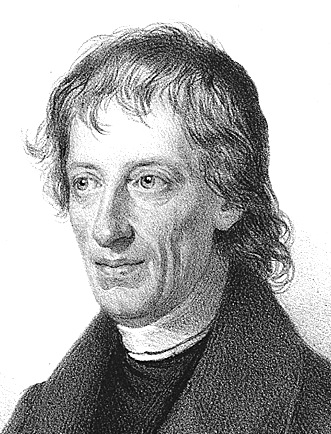
\includegraphics[scale=0.32]{bolzano-abb/portrait.jpg}}}
\noindent Bernard Bolzano war in vielerlei Hinsicht ein außergewöhnlicher Mensch. Als Wissenschaftler verband er so verschiedene Begabungen wie die eines Mathematikers, eines Philosophen, ein"-es Logikers und eines Theologen. Er war katholischer Priester und ein seine Zuhörer begeisternder Hochschullehrer. Er war ein tiefgläubiger Mensch und fühlte sich ganz der Vernunft verpflichtet.  Gedankliche Klarheit, begriffliche Präzision und argumentative Untermauerung seiner Standpunkte galten ihm \anf{als Grundlage für ein vernünftiges, gottgefälliges Leben zum Wohl der Allgemeinheit}.\footnoteA{%
	\lit[11]{Strasser2001}.}
Bolzano ist, dem Philosophen Michael Dummett zufolge, Urgroßvater der analytischen Philosophie.\footnoteA{%
	\lit[167]{Dummett1988}.}
Von ihm stammt der Satz von Bolzano-Weierstraß, den jeder Mathematikstudent heute in seinem ersten Semester 
lernt.\par

\PdUsec{Der Text}
Von der \RWbet{Religionswissenschaft} gibt es fünf Versionen, nämlich 
\begin{compactenum}[1.]
\item[1.] Bolzanos schriftliche Fassung seines ersten Vorlesungszyklus zum Thema;
\end{compactenum}
dann drei Fassungen, die zu Bolzanos Lebzeiten erarbeitet wurden und seine Zustimmung fanden:
\begin{compactenum}[1.]
\item[A] Die 1834 publizierte Fassung,
\item[A$_1$] Bolzanos Überarbeitung von A in seinem Handexemplar sowie
\item[B] Eine im Jahre 1818 erstellte Abschrift seiner Manuskripte für die Studienhofkommission
\end{compactenum}
und schließlich
\begin{compactenum}[1.]
\item[5.] der Text in der Bernard-Bolzano Gesamtausgabe [=GA], Reihe 1, Bände 6/1--2, 7/1--2 und 8/1--4.
\end{compactenum}
Bolzano las seit 1805 regelmäßig einen viersemestrigen Zyklus zur Religionslehre. Der Text des ersten Zyklus ist 1. In den folgenden Jahren überarbeitete Bolzano sein Manuskript stetig. Als er 1818 der Studienhofkommission in Wien seine Arbeiten vorlegen musste, legte er B vor, einen Text, der von einem professionellen Schreiber verfasst, von Bolzano jedoch detailliert korrigiert und im Einzelnen approbiert wurde. 1834 schließlich publizierten Schüler Bolzanos das \RWbet{Lehrbuch der Religionswissenschaft}  (= A) anonym bei Seidel im bayrischen Sulzbach, denn  Bolzano durfte seit seiner Entlassung 1819 im Habsburgerreich nicht mehr publizieren. Bolzano zeigte sich mit dem durch seine Schüler eigenständig redigierten Text relativ einverstanden, wollte aber für eine zweite Auflage Umarbeitungen vornehmen. Zu diesem Zweck ließ er sich ein Exemplar des ersten Bandes vom Buchbinder mit leeren Seiten durchschießen, auf die er seine Überarbeitungen eintrug -- so entstand der Text A$_1$. Der Text der Gesamtausgabe folgt im Wesentlichen A$_1$, gibt aber auch Varianten aus $B$ an.\par
% UNZUVERLASSIGKEIT VON GA
Ein Problem mit der ansonsten äußerst verdienstvollen kritischen Edition der Gesamtausgabe ist jedoch, dass sie häufig nicht zuverlässig ist:
Sinnentstellende Verschreibungen (\zB\ \anf{Richtigkeit} statt korrekt \anf{Nichtigkeit} in RW I 10 oder RW IIIa 18); fehlende gewichtende Zusätze (\zB\ \anf{eine höhere Denkfähigkeit} statt korrekt \anf{eine bedeutend höhere Denkfähigkeit} in RW I 13). Nicht-berücksichtigte Korrekturen von Bolzanos Hand, die Sinnstörungen vermeiden (\zB\ \anf{für Laien bestimmt} (wie in \Alabel ) statt \anf{für Nicht-Theologen bestimmt} in RW I 24).
Daher folgt diese Studienausgabe im Wesentlichen dem Text \Alabel\ der gedruckten Ausgabe von 1834. Nach Möglichkeit werden Bolzanos eigene Verbesserungsvorschläge aus der A$_1$ übernommen. 
Diese Studienausgabe folgt im Wesentlichen dem Text der Gesamtausgabe, d.\,h. der Vorlage \A1label\ bzw. \Alabel , und zwar vor allem aus pragmatischen Gründen. So ist dieser Text relativ gut digitalisierbar. Eine eigene Edition von B machte eine Menge zusätzlichen Aufwands nötig und gehörte wohl eher in die Reihe der unveröffentlichten Schriften in der 
Gesamtausgabe.\par
Grundsätzlich wird aber in Folgendem von der GA abgewichen:
\begin{aufza}
\item Grundsätzlich wird zugunsten des Textumfangs dieser Studienausgabe nur derjenige Text der GA zugrundegelegt, der auch in \Alabel\ bzw. \A1label\ vorkommt. Zusätzliches Material wie die frühere Fassung der Vorrede, das \anf{Vorwort} (GA I 6/1, S. 19--22), oder die vielfältigen Auszüge von Varianten aus B in den Anhängen der Bände der GA werden weggelassen.
\item In \Alabel\ waren nahezu alle Textabsätze durchnummeriert. Die GA löscht diese Nummerierungen (vermutlich, weil Bolzano selbst sie in A$_1$ gelöscht hat) und setzt die Unternummerierungen dafür eine Ebene höher (\dh\ eine nachgeordnete Aufzählung beginnt nun mit arabisch 1., während sie in A mit lateinisch a. begann -- dafür nummeriert arabisch 1. eben den Absatz). Diese Änderung gegenüber A wird jedoch in GA weder verzeichnet noch beschrieben. Sie wird auch nicht durchgehalten, sodass sich ein uneinheitliches Bild ergibt: In GA I 6/1--2 die gegenüber A geänderte Nummerierung, in GA I 7 \& 8 die ursprüngliche Nummerierung aus A. Hier wird die ursprüngliche Nummerierung aus A einheitlich und durchgängig verwendet.
\end{aufza}
Für die konkrete Textgestalt wurden Bolzanos eigene Wünsche, soweit sie aus seinen handschriftlichen Überarbeitungen und Hinweisen in A$_1$ ersichtlich sind, nach Möglichkeit berücksichtigt: 
\zit[{Bolzano in A$_1$, S. 1 am Rande; zit. n. GA I 6/1, S. 41}]{%
Sollte es nicht besser seyn, \auslass\ wenn die §§ Nummern durch das ganze Buch eben neben der Seitenzahl auf jedem Blatte angezeigt würden, wodurch das Nachschlagen erleichtert würde?
}
Am Beginn des Inhaltsverzeichnisses verlangte Bolzano am Ende der Überschriften der Paragraphen 11, 13 und 14, insofern es sich bei diesen und unter den ersten 14 Paragraphen auch nur bei diesen um vollständige Sätze handelte, einen Punkt. Ab Paragraph 15 hingegen hat er das nicht mehr korrigiert, obwohl etwa die Paragraphen 15--18 alle ganze Sätze als Überschriften tragen. Vermutlich hat er diese Korrekturmaxime also wieder aufgegeben. Mithin werden die drei genannten Punkte nicht übernommen.\par
Wenn Bolzano durch inkonsistente Korrekturen die Möglichkeit zur Vereinheitlichung oder sonstiger Verbesserung des Textes gibt, wird sie vorgenommen. So korrigiert er im Inhaltsverzeichnis nicht, dass bei § 23 von \erganf{Offenbarung}, in der ganz parallel gestalteten Überschrift von § 24 jedoch von \erganf{Offenbaren} die Rede ist. In den betreffenden Kapitelüberschriften heißt es später jedoch beide Male \erganf{Offenbaren}, sodass wir dies auch im Inhaltsverzeichnis vereinheitlichen.\par
Wenn aus Bolzanos ausführlicher Korrektur des 1.~Bandes eine klare Intention bzgl. der Schreibungen hervorgeht, wird diese Intention auch in den anderen Bänden umgesetzt. So hat er bspw. aus dem Wort \anf{Willkühr} und Ableitungen wie \anf{unwillkührlich} im 1.~Band konsequent (wenn auch nicht überall, \zB\ nicht im letzten Satz von \RWparnr{137}) das h gestrichen. 

Weitere Hinweise zur Gestaltung dieser Edition:
\begin{aufza}
\item Grundsätzlich bleibt die Orthographie so wie zu Bolzanos Zeit. Dies schränkt die Lesbarkeit kaum ein und vermittelt dem Leser dafür etwas von dem authentischen \anf{Flair} des 19.~Jahrhunderts, wenn er beispielsweise \anf{Princip}, \anf{nöthig} oder \anf{Gesammtglaube} liest. 
\item Bolzano hat Zitate von Texten in der Regel nicht in Anführungszeichen eingeschlossen. (In A werden kaum Anführungszeichen verwendet. Bolzano scheint sie auch nicht in A$_1$ nachgetragen zu haben.) Um die Lesbarkeit und die Identifikation von Zitaten zur erleichtern, werden in dieser Ausgabe Zitate oder zitatnahe Paraphrasen fremder Texte nach Möglichkeit in Anführungszeichen eingeschlossen. Dabei werden deutsche Anführungszeichen (\eanf{\ }) dort verwendet, wo Bolzano selbst Anführungszeichen gesetzt hat. Wir ergänzen hingegen inverse französische Anführungszeichen (\erganf{\ }) als Markierung von Zitaten, etwa wenn im Apparat Literatur nachgewiesen wird. Allerdings muss man stets im Kopf behalten, dass Bolzano häufig eher paraphrasiert als wörtlich zitiert. Dennoch erhöhen diese Zeichen die Lesbarkeit, insofern man schnell sieht, wo das Referat (sei es wörtlich oder paraphrasierend) beginnt und endet. Keine Anführungszeichen werden hingegen dort ergänzt, wo nach heutiger Konvention ein Wort erwähnt und nicht gebraucht wird, und auch dort nicht, wo man wörtliche Rede heute meist in Anführungszeichen setzen würde. Referiert Bolzano beispielsweise eine Passage aus einem sokratischen Dialog, so wird diese Passage als Ganze in Anführungszeichen gesetzt, die einzelnen Redebeiträge der Dialogteilnehmer hingegen nicht. Ebenso wird verfahren bei Jesus-Worten: Sind es biblische Zitate (oder Paraphrasen), so werden die Anführungszeichen \erganf{\ } ergänzt, als wörtliche Rede einer Person hingegen werden keine Anführungszeichen hinzugefügt.
% \erganf verwenden für ergänzte Anführungszeichen, d.h. solche, die nicht in A vorkommen
\item Die Zeichensetzung folgte im 19.~Jahrhundert anderen Üblichkeiten als heute. Bolzano setzt Kommata regelmäßig an Stellen, an denen nach heutigen Regeln keine gesetzt werden, etwa vor \anf{und} und \anf{oder} in Beiordnungen von Sätzen, die ein gemeinsames Subjekt haben, zwischen \anf{sowohl} und \anf{als auch} sowie vor Vergleichen mit \anf{als}. Grundsätzlich bestanden mehr Freiheiten. So setzt Bolzano Kommata auch als rhetorische Untergliederungen ein. Die Zeichensetzung in dieser Ausgabe folgt im Wesentlichen Bolzanos eigener Zeichensetzung in Ausgabe A. Abgewichen wird davon nur, wenn es naheliegt, dass nach Bolzanos mutmaßlichen eigenen Zeichensetzungsprinzipien ein Fehler vorliegt -- wie etwa dann, wenn bei einer Folge offensichtlich beigeordneter Sätze ohne erkennbaren Grund nur einmal ein Semikolon anstelle eines Kommas steht, ein Punkt sowohl vor als auch nach einem eingeklammerten Ausdruck am Satzende steht oder wenn ein Komma am Satzende auftaucht und der Beginn des nächsten Satzes großgeschrieben wird usw. -- oder sich zumindest eine andere Zeichensetzung nach Bolzanos eigener Systematik nahelegt -- wie etwa dann, wenn er eine Reihe von Bibelstellen nach dem Schema \anf{Stellenangabe - Doppelpunkt - Paraphrase} angibt und der Doppelpunkt in Einzelfällen fehlt.
\item Bolzanos spezifische Form, Bibelstellen anzugeben, wird grundsätzlich beibehalten. So setzt er zwischen Kapitel- und Verszahl ein Komma ohne Leerzeichen und schließt die Stellenangabe mit einem Punkt ab, der für heutige Lesegewohnheiten ungewöhnlich ist, aber im Sinne einer Ordnungszahl durchaus Sinn macht: \anf{11,7.} hat er wohl gelesen im Sinne von \anf{Kapitel 11, \RWbet{siebter} Vers}. Ebenfalls zugunsten der besseren Lesbarkeit wird zwischen aufgezählten Bibelstellenangaben ein Satzzeichen eingefügt. Wir schreiben also \anf{1\,Mos.~1,26.; 3,22.; 11,7.} statt \anf{1\,Mos. 1,26. 3,22. 11,7.}
\item Die Orthographie wird weitgehend so belassen, wie Bolzano sie mutmaßlich anwandte. Mithin werden im 19.~Jahrhundert übliche Schreibungen wie \anf{Thal}, \anf{Gesammtheit}, \anf{insgesammt} u.ä. beibehalten. Nur offenkundige grammatikalische oder orthographische Fehler werden berichtigt wie z.B. \anf{Aeußerungen über Gottes dreifache Persönlichkeit} anstatt \anf{\auslass\ dreifacher \auslass}, oder etwa \anf{\RWgriech{basile'ian Jeo~u o>u klhronom'hsousin}} statt \anf{\RWgriech{\auslass\ klhronom'hsousi}} (in RW IIIb 143 ausdrücklich aus der Bibelstelle \RWbibel{1\,Kor}{1\,Kor}{6}{9} zitiert). In relativ eindeutigen Fällen wie diesen, werden die Änderungen  stillschweigend vorgenommen.  Änderungen gegenüber A, bei denen nicht sicher ausgeschlossen werden kann, dass die fehlerhaft scheinende Schreibung irgendeinen Sinn haben könnte, werden im Apparat vermerkt.
\item Nach heutigen Regeln werden am Ende von Überschriften keine Punkte gesetzt. Daher werden die Punkte nach den Überschriften der Paragraphen weggelassen. Da die Überschriften der Hauptteile und anderen größeren Abschnitte jedoch in aller Regel mehrere Teile haben, die eh durch Punkte abzutrennen sind, werden hier zur Vereinheitlichung auch die Endpunkte beibehalten.
\item Einige Besonderheiten ergeben sich aus Bolzanos teilweiser Überarbeitung von \Alabel\ zu \A1label . In \Alabel\ werden Adjektive, die zwischen \anf{alle} und einem Substantiv stehen, wie heute üblich schwach flektiert (\anf{alle christlichen Weltweisen}); gelegentlich hat Bolzano dies in \A1label\ jedoch ausdrücklich zur starken Flexion hin korrigiert (\anf{alle christliche Weltweisen}). Da die starke Flexion nach \anf{alle} heute vollkommen unüblich geworden ist und da Bolzano diese Korrekturen selbst in dem Teil der RW, den er intensiv überarbeitet hat, nicht immer durchführt, weichen wir hier zugunsten der besseren Lesbarkeit von seinem Willen ab und verwenden die schwache Flexion.
\item Sowohl in der Druckfassung \Alabel\  als auch in Bolzanos Überarbeitung \A1label\ wird gelegentlich \anf{allmählich} und gelegentlich \anf{allmählig} geschrieben. Da die Orthographie heute nur noch \anf{allmählich} kennt, wird dahingehend vereinheitlicht. Anders hingegen bei Variationen, bei denen auch heute noch beide Formen als korrekt gelten. So werden Bolzanos Wechsel zwischen \anf{-es} und \anf{-s} bei den Genitiv-Endungen nicht vereinheitlicht (\anf{des Christenthums} und \anf{des Christenthumes}). Dasselbe gilt für den gelegentlichen Ausfall des \anf{e} bei Worten wie \anf{anderen} / \anf{andren}. 
\item Die Informationen über Varianten von \Blabel\ im Verhältnis zu \Alabel\ wurden der \GAlabel\ entnommen. 
\item Auf Nummern von Absätzen oder Ähnlichem wurde in \Alabel\ durchgängig mittels \anf{Nr.} Bezug genommen. Bolzano hat dies in den Teilen, die er überarbeitet hat, konsequent zu einer Graphie geändert, die offenbar für das Lateinische \anf{numero} oder das Französische \anf{numéro} steht: ein \anf{n} mit einem hochgestellten \anf{o} und einem darunterstehenden Punkt. Diese Schreibweise ließ sich nicht eindeutig einer der im europäischen Sprachraum üblichen Varianten wie No, No., N$^{\mathrm{o}}$, n$^{\mathrm{o}}$, n$^{\mathrm{o}}\!.$, n$^{\underline{\mathrm{o}}}$ oder Ähnlichen zuordnen. Daher wurde mit \no\ eine Drucktype entworfen, die seiner eigenen Schreibung möglichst nahekommt.
\item Wenn eine Nummerierung hinzugefügt worden ist, die in \Alabel\ nicht vorkommt, wird dies angemerkt.
\item Einfache Ergänzungen ggü. den Vorlagen werden in eckige Klammern gesetzt ([\auslass ]), bspw. wenn Bolzano RW I 25 eine Fußnote hinzufügt, die mit \anf{gestorben den \auslass} endet, wird das Todesdatum des Betreffenden in eckigen Klammern hinzufügt: \anf{gestorben den [11.\,Oktober 1834]}. Wird hingegen ein ganzes Wort ausgelassen, wird dies in den Anmerkungen vermerkt.
\end{aufza}

\endinput
%
%---Zwischentitelei---
% \cleardoublepage\pagestyle{completelyempty}
\thispagestyle{completelyempty}
%\mbox{}\vfill
\begin{center}\PdUtoc{chapter}{Titelblatt der Originalausgabe}
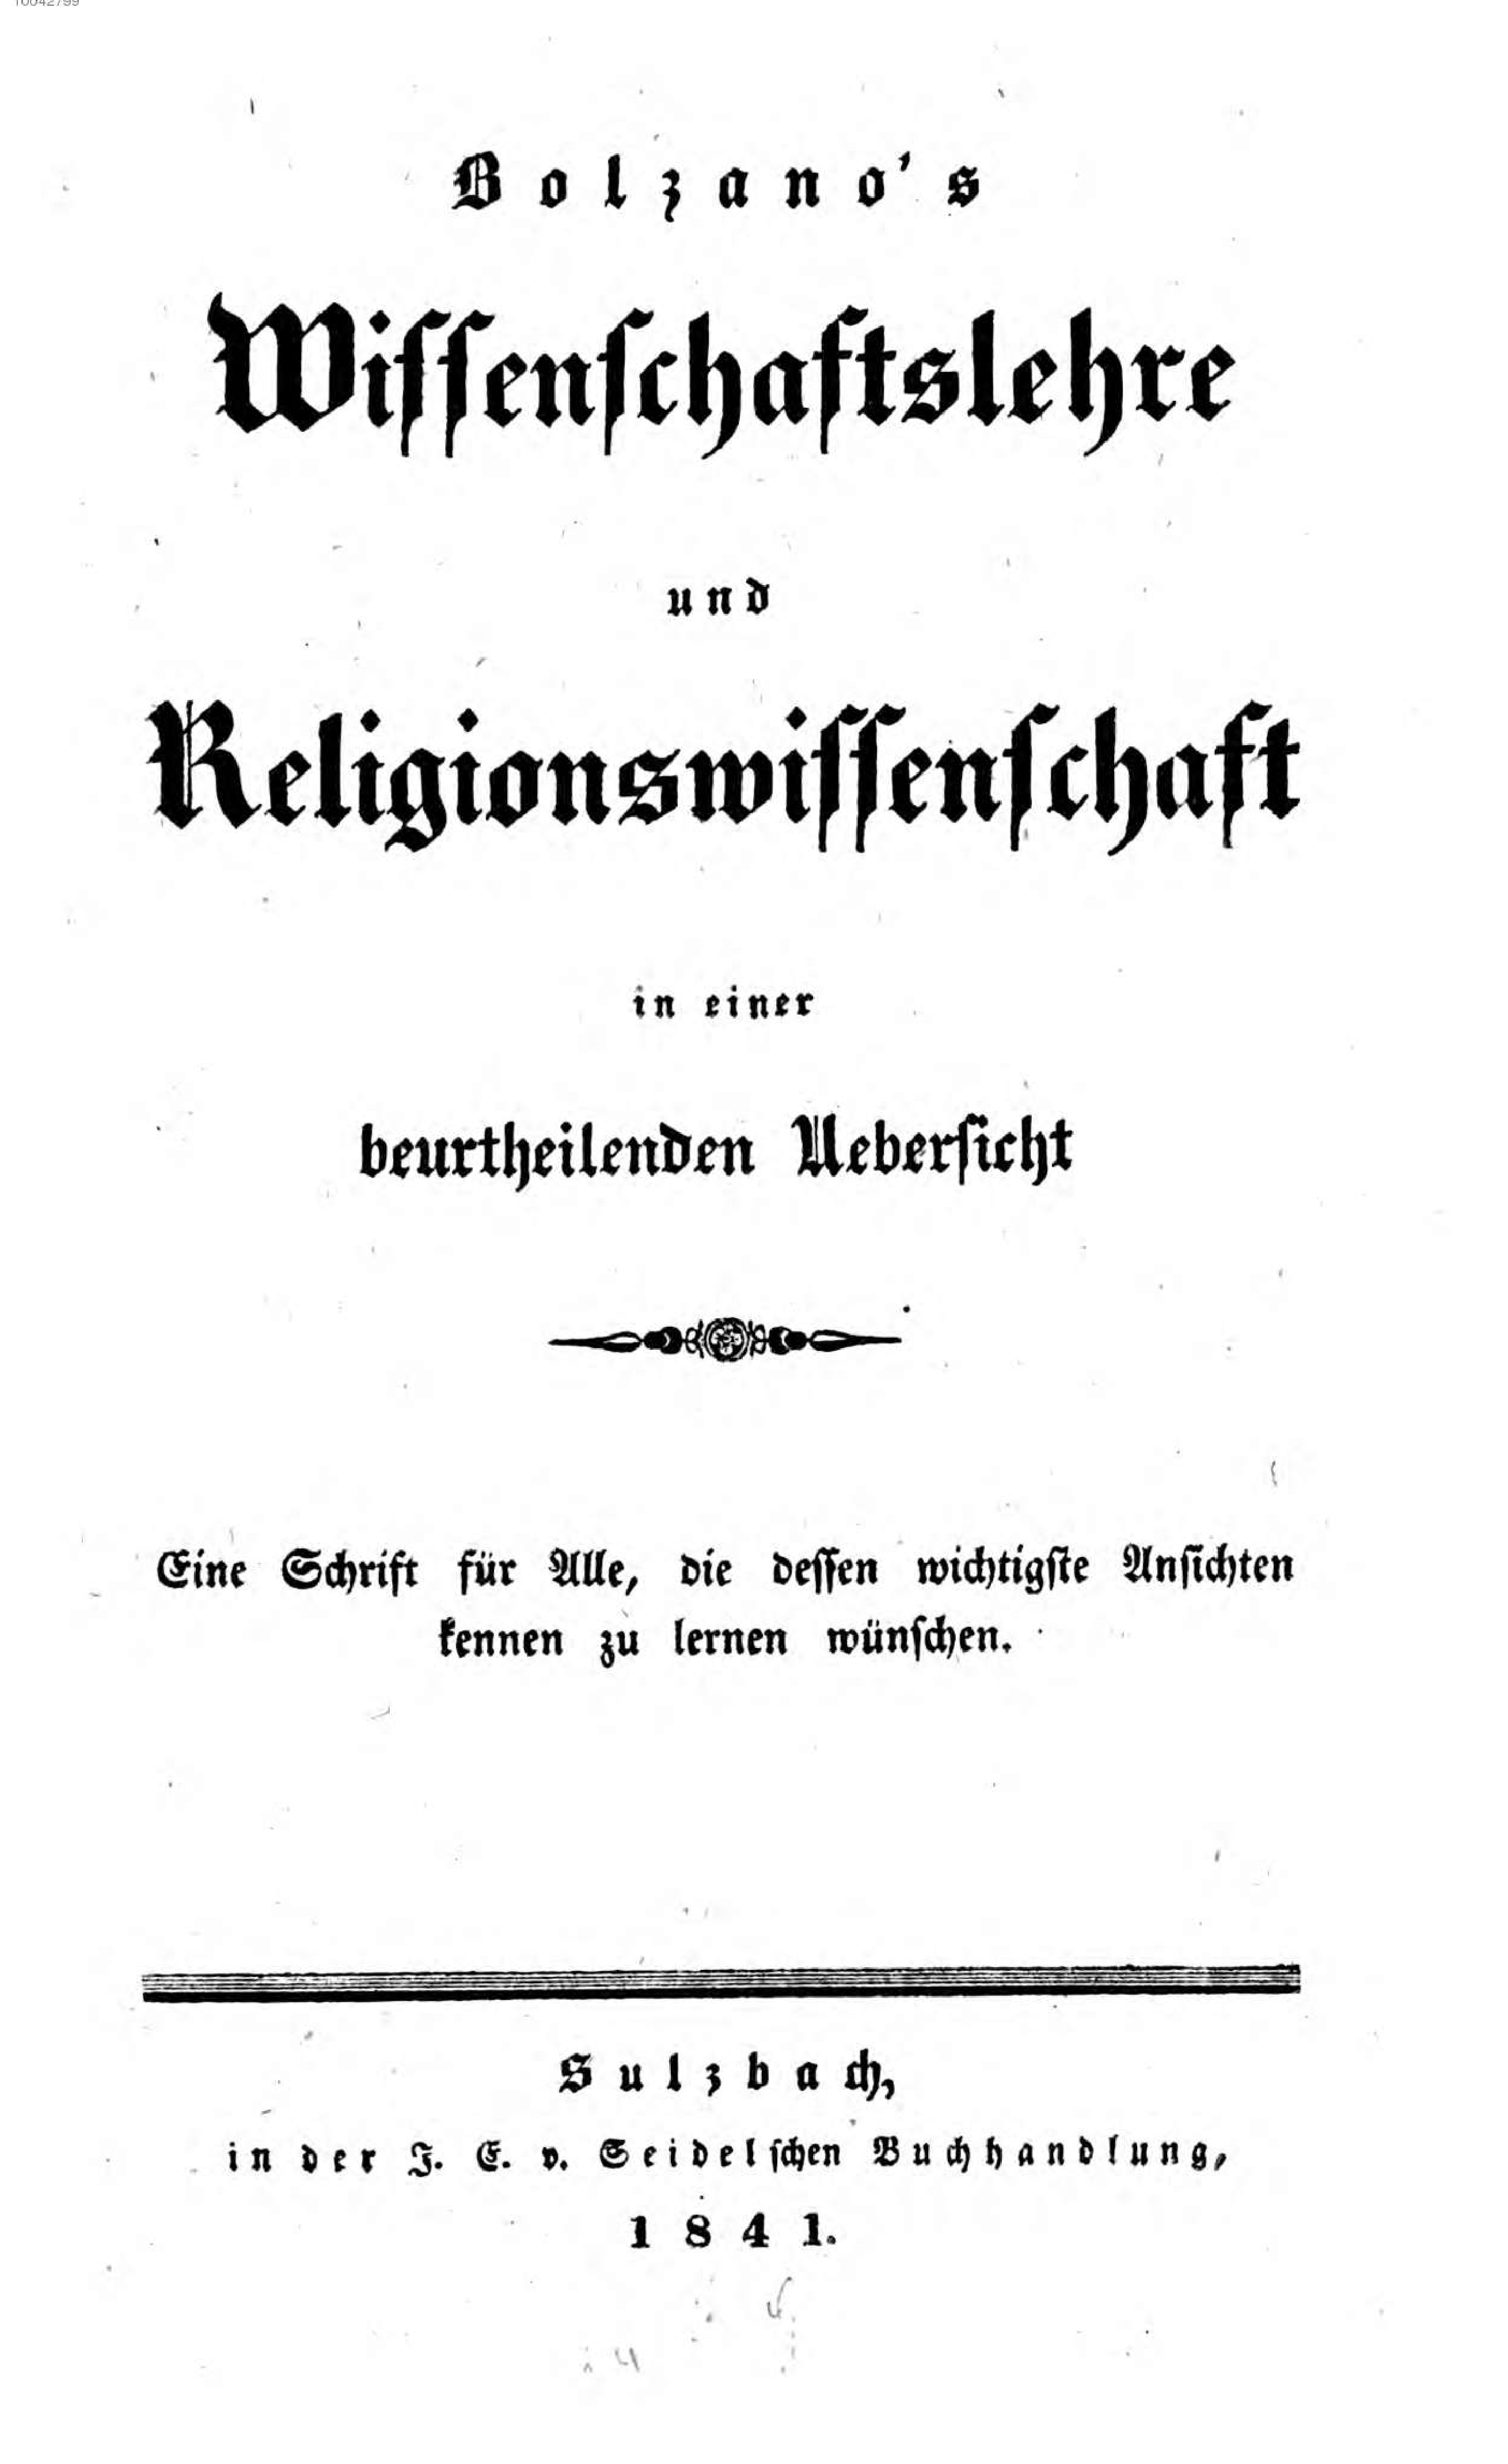
\includegraphics[viewport=2cm 6cm 40.3cm 68.4cm, scale=0.222,clip]{BU_Titel.pdf}
\end{center}
%\vfill
%\clearpage
\neuerechteseite
\endinput
\cleardoublepage\pagestyle{completelyempty}
\thispagestyle{completelyempty}
%\mbox{}\vfill
\begin{center}\PdUtoc{chapter}{Titelblatt der Originalausgabe}
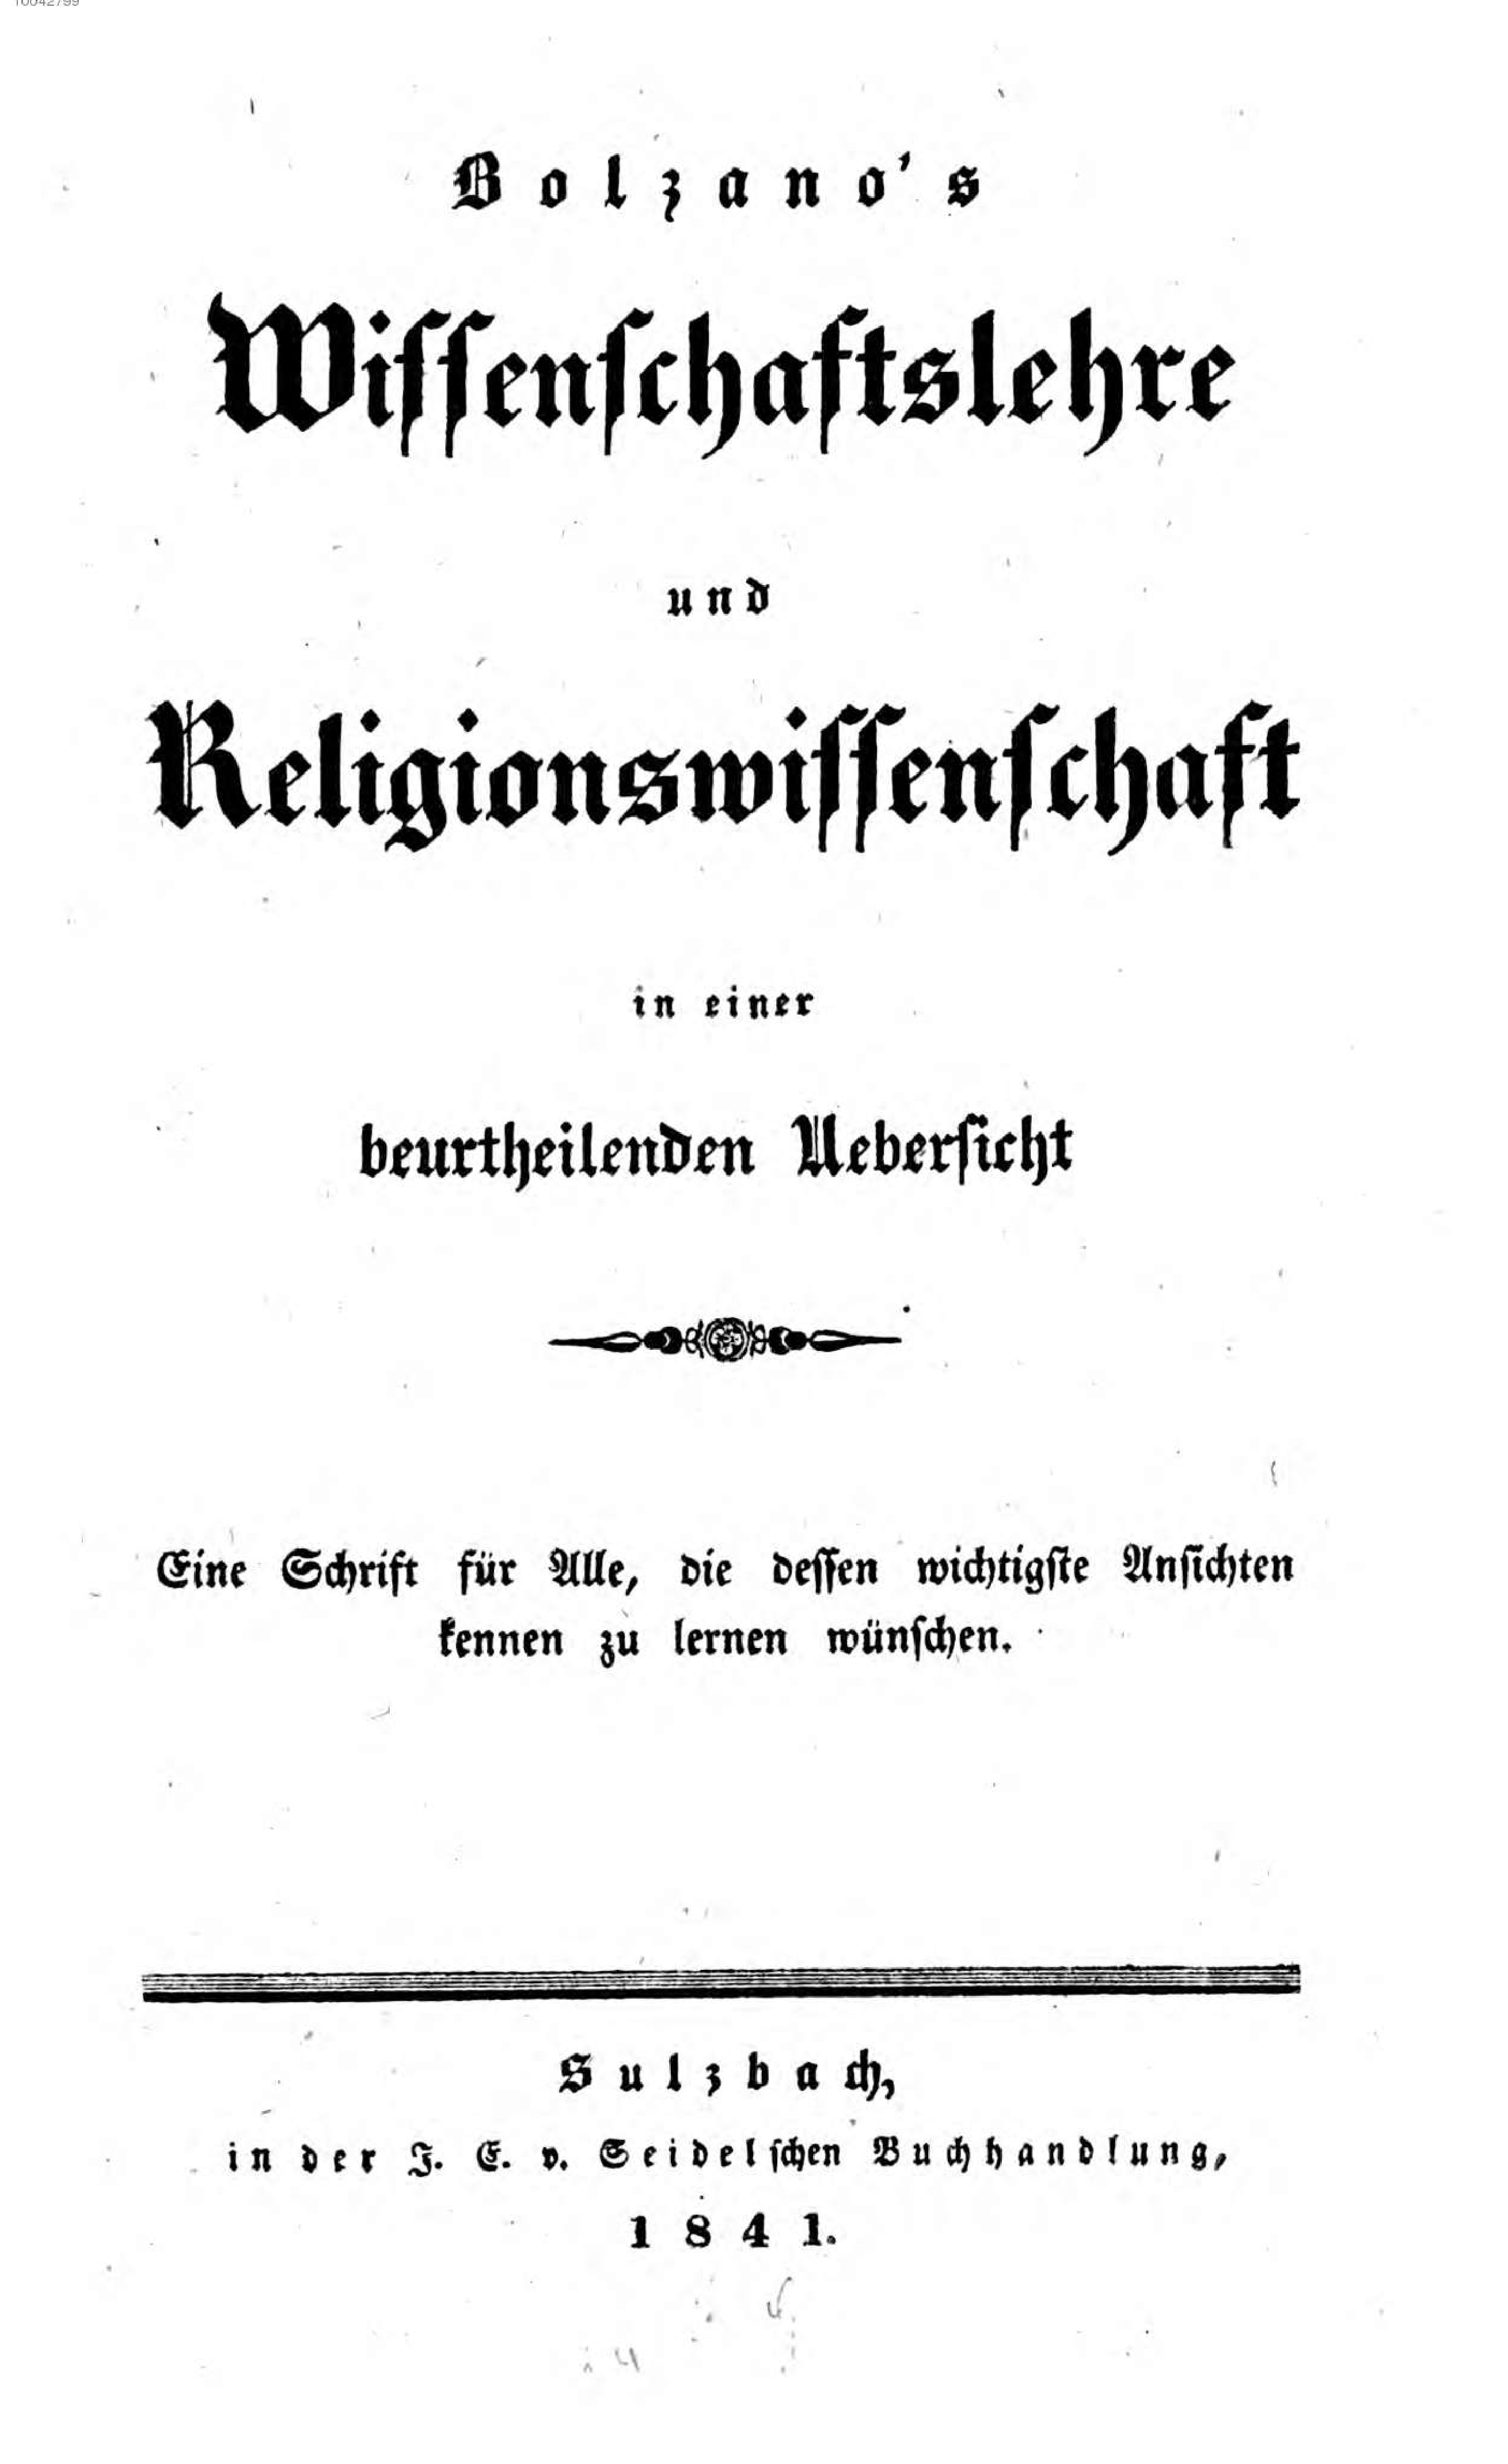
\includegraphics[viewport=2cm 6cm 40.3cm 68.4cm, scale=0.222,clip]{BU_Titel.pdf}
\end{center}
%\vfill
%\clearpage
\neuerechteseite
\endinput
%
%
%---Einleitung---
\RWch{Einleitung des Herausgebers}\hbox{}\par\noindent\markboth{\kopfzeilenfmt{Einleitung des Herausgebers}}{\kopfzeilenfmt{Christian Tapp}}%
% % intro.tex aus dem Projekt PdU
%\RWch{Einleitung}\markboth{\kopfzeilenfmt{Einleitung}}{\kopfzeilenfmt{Christian Tapp}}
\vspace{-1.5\baselineskip}{
\let\footnote\footnoteC
\PdUsec{Der Ausgangstext}
Die \bet{Beurtheilende Übersicht} [=BÜ] -- kurz für: \bet{Bolzano's Wissenschaftslehre und Religionswissenschaft in einer beurtheilenden Uebersicht} -- erschien 1841 bei Seidel in Sulzbach. Im Kern bietet sie eine kurze Zusammenfassung der wichtigsten Gedankengänge aus den beiden Hauptwerken Bernard Bolzanos (1781--1848), nämlich der \bet{Religionswissenschaft} [=RW] von 1834 und der \bet{Wissenschaftslehre} [=WL] von 1837. Ergänzt wird diese Zusammenfassung durch Erläuterungen und Erklärungen, die augenscheinlich Missverständnisse in der (spärlichen) Rezeption dieser beiden Werke ausräumen sollen.

\PdUsec{Die Autorschaft}
Die BÜ ist durchgehend aus der Perspektive eines von Bolzano verschiedenen Autors geschrieben, der Bolzanos Werk \anf{von außen} beschreibt und diskutiert. Dennoch ist allgemeiner Forschungskonsens, dass das Werk bis auf die Einleitung von Bolzano selbst verfasst wurde, während die Einleitung von Bolzanos Schüler und Freund Michael Josef Fesl (1788--1864) verfasst wurde.\par
Bolzanos Autorschaft bezeugt \zB\ \priholang\ (1788--1859), wenn er im Nekrolog Bolzanos [1850] schreibt:
\zit[BGA 4,1/3, S. 216--217]{Für den Zweck der Erläuterung und Empfehlung seiner philosophischen und religiösen Ansichten schrieb B.[olzano] das Büchlein: B.[olzano]'s Wissenschaftslehre und Religionswissenschaft in einer beurtheilenden Uebersicht (Sulzbach 1841). -- Schon aus den Titeln ist zu entnehmen, daß diese Schriften nicht von ihm, sondern von seinen Freunden sind herausgegeben worden und dieß zwar im Auslande mit Umgehung der österr. Censur, die eigens angewiesen war, von ihm nichts durchgehen zu lassen.}
Ähnlich schreibt Fesl (1788--1864) im Jahre 1849 an die Kaiserliche Akademie der Wissenschaften in Wien:
\zit[BGA 4,1/3, S. 190]{Was er auf diesem Gebiete [=dem der Philosophie, C.\,T.] Neues oder Vollkommneres geleistet zu haben glaubte, darüber berichtet er selbst in seiner \anf{Uebersicht der Wissenschaftslehre und Religionswissenschaft} (1841) ebenso aufrichtig als bescheiden.}\par
Die Darstellungen \priho s und Fesls werden dadurch untermauert, dass mehrere Manuskripte des ersten Teils der BÜ von Bolzanos Hand erhalten sind. Sie liegen im Prager Bolzano-Nachlass.\footnote{%
	Signaturen DVb1--DVb3 lt. BGA E 2/3, S. 36.}
Weitere Hinweise auf die Autorschaft finden sich in Zeithammers Biographie (BGA 4,2, S. 155--156), sowie in Bolzanos Briefen an \priho, BGA 3,3/1--3, S. 216, 217, 233.\par
Die Autorschaft Bolzanos hat mithin als gesichert gelten.


\PdUsec{Die Textgestaltung}
Die vorliegende Ausgabe gibt den Text der gedruckten Ausgabe von 1841 wieder. Der Rohtext wurde aus Scans dieser Ausgabe mit Unterstützung des Programms \anf{Transkribus} gewonnen.\par
Bei der Abwägung zwischen originalgetreuer Wiedergabe und guter Lesbarkeit wurden folgende Entscheidungen getroffen:
\begin{aufza}
\item Die für den deutschen Text verwendete Frakturschrift wird durch eine heute übliche Antiqua ersetzt.
\item Es wird grundsätzlich \bet{buchstabengetreu} ediert, \dh
	\begin{aufzb}
	\item Wenn das Original den Buchstaben \anf{ä} hat, wird auch ein \anf{ä} wiedergegeben, auch wenn als Umlautzeichen damals noch häufig ein kleines e über den Vokal geschrieben wurde (\anf{\ensuremath{\mathrm{\overset{\raisebox{-2pt}{\scalebox{0.4}{e}}}{a}}}}). Dies wird also als eine andere Schreibung des Buchstabens \anf{ä} angesehen und mithin als \anf{ä} wiedergegeben. 
	\item Wenn das Original im Fall von Diphthongen, bei denen der erste Buchstabe ein Umlaut ist (v.a. \anf{äu} bzw. \anf{Äu}), das Umlautzeichen auf den zweiten Vokal verschoben hat, wird das beibehalten. Statt \anf{Äußerung} wird also, wie im Originaltext, \anf{Aüßerung} gedruckt, denn die Buchstaben waren dort eben \anf{A} und \anf{ü} und nicht \anf{Ä} und \anf{u}. -- Diese Satzbesonderheit ist für heutige Augen ungewöhnlich. Sie war zur damaligen Zeit aber durchaus regelmäßig anzutreffen und ist auch in der BÜ 1841 durchgängig zu finden. Sie stört den Lesefluss kaum. Ihre Beibehaltung vermittelt  -- gemeinsam mit der vollständig beibehaltenen Orthographie -- das \anf{Flair} eines Drucks aus der ersten Hälfte des 19.~Jahrhunderts. 
	\end{aufzb}
\item Von der buchstabengetreuen Wiedergabe wird nur abgewichen, wenn es sich offensichtlich um echte Druckfehler handelt. Der häufigste Druckfehler in der BÜ ist die Verwechslung von \anf{\textswab{n}} und \anf{\textswab{u}} -- was wohl durch ihre annähernde Rotationssymmetrie erklärlich ist.\footnote{%
	Zum Beispiel: \anf{Verneinnng} statt \anf{Verneinung} (BÜ 65, Z.\,4); \anf{Ansdrücke} statt \anf{Ausdrücke} (BÜ 136, Z.\,38); \anf{deu} statt \anf{den} (BÜ 151, Z.\,29). -- Bei der Zeilenzählung wird stets die Seitennummer im Kolumnentitel als Zeile 1 gezählt.}
\item Entsprechend werden auch weitere Druckfehler korrigiert, sofern es sich offensichtlich um solche handelt, wie etwa bei dem einfachen Anführungszeichen statt eines dopppelten am Zeilenanfang (BÜ 96, Z.\,10), bei der Graphie \fbox{,\grq ,} statt \fbox{,\grqq }, wo vermutlich die dritte Drucktype um 180° gedreht war, (BÜ 100, Z.\,4) oder \anf{und} statt \anf{uns} (BÜ 127, Z.\,23).
\item Was die Setzung von Anführungszeichen angeht, lässt sich Folgendes beobachten.
\begin{aufzb}
\item Grundsätzlich, aber nicht immer, setzt Bolzano\footnote{%
	Der Einfachheit halber wird hier \anf{Bolzano} genannt, ohne damit sagen zu wollen, dass diese Eigentümlichkeiten auf ihn persönlich zurückgehen, und nicht etwa auf die Herausgeber, den Verlag oder den Drucker.}
wörtliche Zitate in Anführungszeichen. 
\item In der BÜ folgt er außerdem der damaligen Gepflogenheit, bei in Anführungszeichen gesetzten Zitaten, die sich über mehrere Zeilen erstrecken, am Beginn jeder neuen Zeile noch einmal ein öffnendes Anführungszeichen zu setzen.
\item Die heute geläufige Praxis, mittels Anführungszeichen zwischen der Erwähnung eines Ausdrucks und seiner Verwendung (d.h. der Erwähnung des durch den Ausdruck Bezeichneten) zu unterscheiden, hat Bolzano nicht geteilt. Wenn er herausstreichen will, dass es gerade um das Wort als Wort geht, so verwendet er eher den \gesperrt{Gesperrtdruck}, den er ganz allgemein als Hervorhebungmarkierung einsetzt. 
\item In dieser Ausgabe werden deutsche Anführungszeichen (\danf{\ }) verwendet, wenn in der Vorlage Anführungszeichen gesetzt sind (dies sind i.d.R. auch deutsche Anführungszeichen). Falls Anführungszeichen hingegen aus Gründen der Verständlichkeit hinzugefügt werden, werden dazu wie dieselben inversen französischen Anführungszeichen (\anf{\ }) verwendet, wie sie in den Textbeiträgen des Herausgebers als Anführungszeichen benutzt werden.
\item Wenn Bolzano, wie etwa in BÜ 92 ein Zitat-im-Zitat in eigene Anführungszeichen setzt, verwendet er dazu auch die doppelten deutschen Anführungszeichen, sodass die Graphie am Zeilenanfang entsprechend \fbox{\glqq\glqq} lautet. Wir ersetzen, heutigen Gepflogenheiten entsprechend, bei Zitaten-im-Zitat die doppelten durch einfache deutsche Anführungszeichen (\deinfanf{\ }).
\end{aufzb}
\item Ergänzungen des Herausgebers werden durch eckige Klammern (\erg{\ }) markiert.
\item Zur Orientierung in diesem Band:
\begin{aufzb}
\item In den Kolumnentiteln werden links das Bezugswerk und die Bandnummer genannt (z. B. \anf{Zu WL III} bedeutet: zum dritten Band der Wissenschaftslehre). 
\item Die Wissenschaftslehre weist Paragraphenzählungen auf, die über die Bandgrenzen fortlaufen. Außerdem bespricht Bolzano sie chronologisch. Daher können Paragraphenangaben im rechten Kolumnentitel hier die Orientierung erleichtern. 
\item Die Religionswissenschaft hat hingegen in jedem Haupttheil neue Paragraphenzählungen und Bolzano bespricht sie nicht chronologisch, sondern mit veränderter Reihenfolge zwischen manchen Hauptstücken. Daher werden hier im rechten Kolumnentitel die Nummer und der Paragraphenbereich des betreffenden Hauptstücks angeführt. Zusätzlich werden die Angabe des \RWHSfmt{Hauptstücks} und seines \RWHSfmt{Titels} im Text unterstrichen.
\item Bolzano verwendet zwar häufig Anführungszeichen, wenn er aus seinen eigenen Werken zitiert, dies bedeutet aber nicht unbedingt, dass der Text wortgetreu wiedergegeben wird. Zitate, bei denen nur zusammengefasst oder stilistisch verändert wurde, werden so belassen. Sind hingegen größere, u.\,U. inhaltlich relevante Änderungen gegenüber dem zitierten Text festzustellen, werden die Änderungen editorisch kenntlich gemacht.
\end{aufzb}
\end{aufza}
}
\endinput
% intro.tex aus dem Projekt PdU
%\RWch{Einleitung}\markboth{\kopfzeilenfmt{Einleitung}}{\kopfzeilenfmt{Christian Tapp}}
\vspace{-1.5\baselineskip}{
\let\footnote\footnoteC
\PdUsec{Der Ausgangstext}
Die \bet{Beurtheilende Übersicht} [=BÜ] -- kurz für: \bet{Bolzano's Wissenschaftslehre und Religionswissenschaft in einer beurtheilenden Uebersicht} -- erschien 1841 bei Seidel in Sulzbach. Im Kern bietet sie eine kurze Zusammenfassung der wichtigsten Gedankengänge aus den beiden Hauptwerken Bernard Bolzanos (1781--1848), nämlich der \bet{Religionswissenschaft} [=RW] von 1834 und der \bet{Wissenschaftslehre} [=WL] von 1837. Ergänzt wird diese Zusammenfassung durch Erläuterungen und Erklärungen, die augenscheinlich Missverständnisse in der (spärlichen) Rezeption dieser beiden Werke ausräumen sollen.

\PdUsec{Die Autorschaft}
Die BÜ ist durchgehend aus der Perspektive eines von Bolzano verschiedenen Autors geschrieben, der Bolzanos Werk \anf{von außen} beschreibt und diskutiert. Dennoch ist allgemeiner Forschungskonsens, dass das Werk bis auf die Einleitung von Bolzano selbst verfasst wurde, während die Einleitung von Bolzanos Schüler und Freund Michael Josef Fesl (1788--1864) verfasst wurde.\par
Bolzanos Autorschaft bezeugt \zB\ \priholang\ (1788--1859), wenn er im Nekrolog Bolzanos [1850] schreibt:
\zit[BGA 4,1/3, S. 216--217]{Für den Zweck der Erläuterung und Empfehlung seiner philosophischen und religiösen Ansichten schrieb B.[olzano] das Büchlein: B.[olzano]'s Wissenschaftslehre und Religionswissenschaft in einer beurtheilenden Uebersicht (Sulzbach 1841). -- Schon aus den Titeln ist zu entnehmen, daß diese Schriften nicht von ihm, sondern von seinen Freunden sind herausgegeben worden und dieß zwar im Auslande mit Umgehung der österr. Censur, die eigens angewiesen war, von ihm nichts durchgehen zu lassen.}
Ähnlich schreibt Fesl (1788--1864) im Jahre 1849 an die Kaiserliche Akademie der Wissenschaften in Wien:
\zit[BGA 4,1/3, S. 190]{Was er auf diesem Gebiete [=dem der Philosophie, C.\,T.] Neues oder Vollkommneres geleistet zu haben glaubte, darüber berichtet er selbst in seiner \anf{Uebersicht der Wissenschaftslehre und Religionswissenschaft} (1841) ebenso aufrichtig als bescheiden.}\par
Die Darstellungen \priho s und Fesls werden dadurch untermauert, dass mehrere Manuskripte des ersten Teils der BÜ von Bolzanos Hand erhalten sind. Sie liegen im Prager Bolzano-Nachlass.\footnote{%
	Signaturen DVb1--DVb3 lt. BGA E 2/3, S. 36.}
Weitere Hinweise auf die Autorschaft finden sich in Zeithammers Biographie (BGA 4,2, S. 155--156), sowie in Bolzanos Briefen an \priho, BGA 3,3/1--3, S. 216, 217, 233.\par
Die Autorschaft Bolzanos hat mithin als gesichert gelten.


\PdUsec{Die Textgestaltung}
Die vorliegende Ausgabe gibt den Text der gedruckten Ausgabe von 1841 wieder. Der Rohtext wurde aus Scans dieser Ausgabe mit Unterstützung des Programms \anf{Transkribus} gewonnen.\par
Bei der Abwägung zwischen originalgetreuer Wiedergabe und guter Lesbarkeit wurden folgende Entscheidungen getroffen:
\begin{aufza}
\item Die für den deutschen Text verwendete Frakturschrift wird durch eine heute übliche Antiqua ersetzt.
\item Es wird grundsätzlich \bet{buchstabengetreu} ediert, \dh
	\begin{aufzb}
	\item Wenn das Original den Buchstaben \anf{ä} hat, wird auch ein \anf{ä} wiedergegeben, auch wenn als Umlautzeichen damals noch häufig ein kleines e über den Vokal geschrieben wurde (\anf{\ensuremath{\mathrm{\overset{\raisebox{-2pt}{\scalebox{0.4}{e}}}{a}}}}). Dies wird also als eine andere Schreibung des Buchstabens \anf{ä} angesehen und mithin als \anf{ä} wiedergegeben. 
	\item Wenn das Original im Fall von Diphthongen, bei denen der erste Buchstabe ein Umlaut ist (v.a. \anf{äu} bzw. \anf{Äu}), das Umlautzeichen auf den zweiten Vokal verschoben hat, wird das beibehalten. Statt \anf{Äußerung} wird also, wie im Originaltext, \anf{Aüßerung} gedruckt, denn die Buchstaben waren dort eben \anf{A} und \anf{ü} und nicht \anf{Ä} und \anf{u}. -- Diese Satzbesonderheit ist für heutige Augen ungewöhnlich. Sie war zur damaligen Zeit aber durchaus regelmäßig anzutreffen und ist auch in der BÜ 1841 durchgängig zu finden. Sie stört den Lesefluss kaum. Ihre Beibehaltung vermittelt  -- gemeinsam mit der vollständig beibehaltenen Orthographie -- das \anf{Flair} eines Drucks aus der ersten Hälfte des 19.~Jahrhunderts. 
	\end{aufzb}
\item Von der buchstabengetreuen Wiedergabe wird nur abgewichen, wenn es sich offensichtlich um echte Druckfehler handelt. Der häufigste Druckfehler in der BÜ ist die Verwechslung von \anf{\textswab{n}} und \anf{\textswab{u}} -- was wohl durch ihre annähernde Rotationssymmetrie erklärlich ist.\footnote{%
	Zum Beispiel: \anf{Verneinnng} statt \anf{Verneinung} (BÜ 65, Z.\,4); \anf{Ansdrücke} statt \anf{Ausdrücke} (BÜ 136, Z.\,38); \anf{deu} statt \anf{den} (BÜ 151, Z.\,29). -- Bei der Zeilenzählung wird stets die Seitennummer im Kolumnentitel als Zeile 1 gezählt.}
\item Entsprechend werden auch weitere Druckfehler korrigiert, sofern es sich offensichtlich um solche handelt, wie etwa bei dem einfachen Anführungszeichen statt eines dopppelten am Zeilenanfang (BÜ 96, Z.\,10), bei der Graphie \fbox{,\grq ,} statt \fbox{,\grqq }, wo vermutlich die dritte Drucktype um 180° gedreht war, (BÜ 100, Z.\,4) oder \anf{und} statt \anf{uns} (BÜ 127, Z.\,23).
\item Was die Setzung von Anführungszeichen angeht, lässt sich Folgendes beobachten.
\begin{aufzb}
\item Grundsätzlich, aber nicht immer, setzt Bolzano\footnote{%
	Der Einfachheit halber wird hier \anf{Bolzano} genannt, ohne damit sagen zu wollen, dass diese Eigentümlichkeiten auf ihn persönlich zurückgehen, und nicht etwa auf die Herausgeber, den Verlag oder den Drucker.}
wörtliche Zitate in Anführungszeichen. 
\item In der BÜ folgt er außerdem der damaligen Gepflogenheit, bei in Anführungszeichen gesetzten Zitaten, die sich über mehrere Zeilen erstrecken, am Beginn jeder neuen Zeile noch einmal ein öffnendes Anführungszeichen zu setzen.
\item Die heute geläufige Praxis, mittels Anführungszeichen zwischen der Erwähnung eines Ausdrucks und seiner Verwendung (d.h. der Erwähnung des durch den Ausdruck Bezeichneten) zu unterscheiden, hat Bolzano nicht geteilt. Wenn er herausstreichen will, dass es gerade um das Wort als Wort geht, so verwendet er eher den \gesperrt{Gesperrtdruck}, den er ganz allgemein als Hervorhebungmarkierung einsetzt. 
\item In dieser Ausgabe werden deutsche Anführungszeichen (\danf{\ }) verwendet, wenn in der Vorlage Anführungszeichen gesetzt sind (dies sind i.d.R. auch deutsche Anführungszeichen). Falls Anführungszeichen hingegen aus Gründen der Verständlichkeit hinzugefügt werden, werden dazu wie dieselben inversen französischen Anführungszeichen (\anf{\ }) verwendet, wie sie in den Textbeiträgen des Herausgebers als Anführungszeichen benutzt werden.
\item Wenn Bolzano, wie etwa in BÜ 92 ein Zitat-im-Zitat in eigene Anführungszeichen setzt, verwendet er dazu auch die doppelten deutschen Anführungszeichen, sodass die Graphie am Zeilenanfang entsprechend \fbox{\glqq\glqq} lautet. Wir ersetzen, heutigen Gepflogenheiten entsprechend, bei Zitaten-im-Zitat die doppelten durch einfache deutsche Anführungszeichen (\deinfanf{\ }).
\end{aufzb}
\item Ergänzungen des Herausgebers werden durch eckige Klammern (\erg{\ }) markiert.
\item Zur Orientierung in diesem Band:
\begin{aufzb}
\item In den Kolumnentiteln werden links das Bezugswerk und die Bandnummer genannt (z. B. \anf{Zu WL III} bedeutet: zum dritten Band der Wissenschaftslehre). 
\item Die Wissenschaftslehre weist Paragraphenzählungen auf, die über die Bandgrenzen fortlaufen. Außerdem bespricht Bolzano sie chronologisch. Daher können Paragraphenangaben im rechten Kolumnentitel hier die Orientierung erleichtern. 
\item Die Religionswissenschaft hat hingegen in jedem Haupttheil neue Paragraphenzählungen und Bolzano bespricht sie nicht chronologisch, sondern mit veränderter Reihenfolge zwischen manchen Hauptstücken. Daher werden hier im rechten Kolumnentitel die Nummer und der Paragraphenbereich des betreffenden Hauptstücks angeführt. Zusätzlich werden die Angabe des \RWHSfmt{Hauptstücks} und seines \RWHSfmt{Titels} im Text unterstrichen.
\item Bolzano verwendet zwar häufig Anführungszeichen, wenn er aus seinen eigenen Werken zitiert, dies bedeutet aber nicht unbedingt, dass der Text wortgetreu wiedergegeben wird. Zitate, bei denen nur zusammengefasst oder stilistisch verändert wurde, werden so belassen. Sind hingegen größere, u.\,U. inhaltlich relevante Änderungen gegenüber dem zitierten Text festzustellen, werden die Änderungen editorisch kenntlich gemacht.
\end{aufzb}
\end{aufza}
}
\endinput
%
%---Zwischentitelei---
% \include{BU_Zwititel}
\input{BU_Zwititel}
%
% Fußnoten umstellen
\makeatletter
\renewcommand{\@makefntext}[1]{\noindent \@makefnmark\hspace{0.33em}#1}
\makeatother
\haupttexttrue%
%
\ctaddtocontents{ptoc}{\protect\vspace{2ex}\protect\normalfont\protect\large\noindent Bolzano's Wissenschaftslehre und Religions- \\ wissenschaft in einer beurtheilenden Übersicht\protect\par}%


%---HAUPTTEXT---
\setcounter{footnote}{0}\renewcommand{\thefootnote}{\fnsymbol{footnote}}%
 \tocgross\pagestyle{normal}
\RWteil{I}{\ensuremath{[}0.}{Einleitung\ensuremath{]}}{\seitenwohne{1}}
 \tocklein
\fi
\global\zeilennummerntrue\clearpage\ifnackt\else\linenumbers\fi%
%\PdUsec{[BÜ 3--15]}
\thispagestyle{ctplain}\noindent\seitenwohne{3}Wer seinen Ansichten, sey es auf dem Wege der mündlichen Unterweisung oder durch Schrift, Eingang bei Andern und allmäliche Verbreitung zu verschaffen wünschet, muß seine Behauptungen nicht nur auf Vordersätze stützen, die Allen einleuchten, sondern auch dafür sorgen, daß es von seinen Zuhörern oder Lesern wahrgenommen werde, sein Schlußsatz stütze sich in der That nur auf diese und sonst keine andern Voraussetzungen. Dieß aber wird bloß dadurch, daß wir in unsern Beweisführungen keiner unnöthigen Sätze erwähnend, nur das allein zur Sprache bringen, was als ein wirklicher Vordersatz zu unserm Schlußsatze führt, noch eben nicht immer erreicht; besonders nicht bei Lesern oder Hörern, welche im Denken noch ungeübt sind, oder -- was schlimmer ist -- des aufrichtigen Willens, zur Erkenntniß der Wahrheit und zu einer festen Ueberzeugung von ihr zu gelangen, ermangeln. \par
Eigentlich wäre nöthig, daß wir bei einer jeden Gelegenheit sagten, und nicht bloß sagten, sondern durch eine darüber eigens angestellte Betrachtung bei jedem unserer Beweise anschaulich machten, daß und wie nach außer den wenigen von uns so eben angezogenen Sätzen nichts Anderes als wahr vorausgesetzt zu werden brauche von Allem, was wir in unserm vorhergehenden Unterrichte behauptet hatten. Mit einer so großen Weitschweifigkeit können wir aber höchstens zu Werke gehen in einer Unterweisung, welche wir mündlich ertheilen: in Schriften müssen wir uns aus mehr als Einem Grunde kürzer fassen; und schon um deßwillen bleibt es in Büchern ungleich mehr als beim mündlichen Vortrage der \seitenw{4} eigenen Denkfertigkeit, ja dem bloßen guten Willen der Leser anheimgestellt, ob und in welchem Grade sie auch bei den triftigsten Beweisen, welche wir ihnen vorlegen, von der Wahrheit unserer Lehren Ueberzeugung gewinnen. Daher ist es besonders bei Werken eines größeren Umfangs und in systematischer Form eine nur zu gewöhnliche Erscheinung, daß Leser, denen nicht Alles, was wir darin zu behaupten wagen, vollkommen klar und bis zur unwidersprechlichen Gewißheit einleuchtend geworden war, der Meinung leben, sie dürften auch den Satz, dessen Beweis wir uns zur Hauptaufgabe gemacht, der gleichsam den Schluß des Ganzen bildet, nicht als befriedigend erwiesen ansehen; und daß sie Solches wähnen, selbst wenn sie bei einiger Aufmerksamkeit wohl hätten abnehmen mögen, daß alle die Sätze, an deren Beweise sie noch etwas vermißt hatten, zu jenem Hauptsatze eben nicht in dem Verhältnisse unentbehrlicher Vordersätze gestanden. Wer sieht nicht, wie sehr dieser einzige Umstand die Verbreitung neuer Wahrheiten erschweret und verzögert, wenn sie auf keine andere Weise als durch ein Buch mitgetheilt werden dürfen!\par
Und doch gibt es der Umstände, die hier hemmend entgegentreten, noch manche andere. Wer weiß es nicht, wie viele Schwierigkeiten es hat, bei der ungeheueren Menge von Schriften, die jede Messe zu Tage gefördert werden, der eigenen, wenn auch noch so gediegenen Arbeit eine nur mäßige Anzahl aufmerksamer Leser zu verschaffen, will man sich keiner Mittel, die der Bescheidene verschmäht, bedienen? Welch eine leichte Sache doch ist's für die Herausgeber gelehrter Zeitschriften und deren Mitarbeiter, auch das gehaltreichste Werk, wenn sie es wollen, der Aufmerksamkeit des Publicums zu entrücken? Wen trifft es nicht, besonders wenn er nicht einmal sich zu nennen braucht, die gelehrte Welt zu versichern, daß ein in Rede stehendes Product nichts Neues enthalte oder daß all das Neue desselben keine Beachtung verdiene?\par
Und wird denn einer solchen Versicherung nicht um so lieber geglaubt, wenn man sie mit der schmeichelhaften Erklärung verbindet, daß die Leser sich lange schon zu einer weit höheren Stufe der Wissenschaft, als der Verfasser jenes Buches, emporgeschwungen haben? -- Ferner, wie schwer gehen doch wir \seitenw{5} Alle -- auch die Gelehrten, wenn ich nicht irre -- daran, wenn wir uns einmal an gewisse Ansichten gewöhnt, uns wieder loszureißen von ihnen, und den Werth einer erst später uns bekannt gewordenen gerecht zu würdigen? Ansichten aber, die nur ein Buch vorträgt, werden sie uns nicht insgemein erst bekannt, nachdem wir schon allerlei ihnen Entgegenstehendes eingelernt haben? Wer begreift endlich nicht, daß bei dem mündlichen Unterrichte gar manche in der Seele des Zuhörers sich erhebende Zweifel und Einwürfe gleich auf der Stelle sich beseitigen lassen, die der Verfasser eines Buches selbst wenn er sie vorhersah, nur der Weitläufigkeit wegen nicht anführen und beantworten durfte, was denn zur Folge hat, daß bei dem bloßen Lesen so oft die Ueberzeugung ausbleibt, die wohl zu Stande gekommen wäre, wenn wir denselben Mann über seinen Gegenstand mündlich hätten vernehmen können! Wer nun dieß Alles, und noch Manches, das wir hier unberührt lassen, erwäget, dem wird es klar werden, mit welchen überwiegenden Schwierigkeiten derjenige zu kämpfen habe, der einer neuen Lehre Gattung und Anerkennung zu erringen strebt, wenn ihm kein anderes Mittel, um sich Gehör zu verschaffen, als das des stummen Buchstabens, zu Gebote stehet, und alle mündliche Mittheilung, gleichviel aus welchem Grunde, versagt 
ist.\par
In dieser Lage, oder vielmehr noch in einer beträchtlich schlimmeren, befindet sich Bolzano, so ferne er den Wunsch hegt, seinen in die Gebiete der Philosophie und Theologie einschlagenden eigenthümlichen Ansichten auch nur so viel Aufmerksamkeit zu verschaffen, als zu einer endlichen Entscheidung über ihren Werth oder Unwerth erforderlich wäre. Nicht nur ihm selbst, sondern auch allen seinen ehemaligen Schülern und Anhängern ist -- wir wissen nicht recht, warum? -- bereits seit einem Zeitraume von vollen zwanzig Jahren, nicht nur ein jeder mündliche Vortrag seiner Ansichten untersagt; sondern sogar durch Schriften können nur ein und der andere seiner im Auslande lebenden Freunde bloß dadurch etwas thun, daß sie sich nothge\seitenw{6}gedrungen des so verdächtigen Mittels der Anonymität bedienen. Nur schüchtern wagten sie es im J.~1827 seine \danf{Athanasia oder Gründe für die Unsterblichkeit der Seele;} in einem langen Zeitraume darauf, 1834 das \danf{Lehrbuch der Religionswissenschaft,} und endlich im Spätherbst des J.~1837 die \danf{Wissenschaftslehre} -- bei den zwei ersteren Werken nicht einmal den Namen des Verfassers angebend -- durch die Bereitwilligkeit der J. E. v. Seidelschen Buchhandlung in Sulzbach an's Licht zu stellen. Welch eine Aufnahme nun diese Werke, in denen ein eigenthümliches philosophisch-theologisches System in seinen Grundzügen dargelegt ist, bis jetzt erfahren haben, das wird mit Mehrerem erzählt in dem \danf{Anhange zur zweiten Auflage der Athanasia, enthaltend eine kritische Übersicht der Literatur über Unsterblichkeit seit 1827} (Sulzbach, 1838), und in der Schrift: \danf{Bolzano und seine Gegner, Ein Beitrag zur neuesten Literaturgeschichte.} (Sulzbach, 1839.) Wer diese kleinen Schriften, die erste nöthigenfalls nur von S.\,99 bis 114 durchlesen will, der wird auf's Klärste dargethan finden, daß bis jetzt keine einzige der vielen eigenthümlichen Lehren, welche B.\ in den genannten drei Werken aufgestellt hat, auch nur von Einem Gelehrten auf eine wissenschaftliche Weise geprüft, und ein Versuch zu ihrer Widerlegung gemacht worden sey. Nun wissen wir zwar recht wohl, es könne auch ephemere Erscheinungen von einer so gänzlichen Werthlosigkeit geben, daß es zu ihrer verdienten Abfertigung wirklich nicht nöthig ist, alle Sonderbarkeiten derselben im Einzelnen herauszuheben, und sich in eine umständliche Widerlegung derselben einzulassen; weil ja das Publicum einmal auch wohl einem Berichterstatter, der sich bei hundert andern Gelegenheiten als einen gewissenhaften Mann bereits erwiesen hat, auf sein Wort glauben darf, daß sich in dieser Schrift auch nicht Ein Körnchen brauchbarer Wahrheit befinde. Aber ist etwa das der Fall bei den Werken B.'s? Wo hätte denn irgend ein achtbarer \Hgkorr{Gelehrte}{Gelehrter} den Muth gehabt zu sagen, die eigenthümlichen philosophischen, oder auch nur die theologischen Begriffe, \seitenw{7}  welche B. in seinen Schriften entwickelt, verdienten es gar nicht, näher geprüfet zu werden? Nein, wir gehen Alles durch, was für oder wider diese Schriften seit ihrer Erscheinung bis auf den heutigen Tag vorgebracht worden ist; wir  überschauen alle günstige und widrige Schicksale, die sie bis jetzt erlebten: und wir behaupten kühn: einen viel höheren  Werth, als der Verfasser selbst ihnen je wünschte beigelegt zu sehen, könnten die Schriften B.'s besitzen; das große Wort,  welches das Räthsel der Gegenwart löst, könnten sie darbieten: und dennoch hätten sie auf keine andere, namentlich  bessere Weise, als es bisher geschah, empfangen werden müssen. Schon daß B.'s Begriffe zu ihrer Verbreitung des Mittels aller mündlichen Gedankenmittheilung entbehren müssen;  daß es keine Lehrstühle gibt, von welchen herab sie einer aus  allen Gegenden Deutschlands herbeiströmenden Jugend vorgetragen werden, verstattet, wie wir gesehen, kein schnelles  Vordringen derselben. Damit vereiniget sich aber noch eine  Menge anderer mißlicher Umstände. B.'s Hauptwerk, die  \danf{Wissenschaftslehre,} welche ihn eigentlich erst darüber zu rechtfertigen vermag, warum er in seiner \danf{Athanasia}  sowohl als in der \danf{Religionswissenschaft} eine von  den jetzt herrschenden so durchaus abweichende Weise zu philosophiren befolgt hat, erschien nicht vor, sondern nach diesen  Schriften, und liegt dem Publico erst zwei Jahre und einige  Monate vor; ein Zeitraum, innerhalb dessen es einem Gelehrten, der sich nicht eben nach Beiseitelegung aller anderer Arbeiten mit diesem Werke allein beschäftigen konnte, noch gar  nicht möglich war, alle in den vier starken Bänden enthaltene  neue Behauptungen, alle denselben beigegebene Gründe, und  Alles, was zur Widerlegung der entgegenstehenden Ansichten  Anderer vorgebracht wird, kennen zu lernen. Daher denn  auch, daß noch kein Mann vom Fache, kein Einziger derjenigen, die in der Philosophie selbst einen Namen sich erworben haben, bis jetzt noch seine belehrende Stimme für oder wider  das Buch zu vernehmen gegeben. Jene Wenigen, die sich  bisher in einem wegwerfenden Tone über dasselbe geäußert,  sorgten schon durch die Eile, mit der sie ihr Urtheil abgaben,  mehr noch aber durch ihre schlecht verhüllte Leidenschaftlichkeit   \seitenw{8} dafür, jeden Vernünftigen über den Werth, welchen er ihrem anonymen Ausspruche beilegen dürfe, zu enttäuschen.\BUfootnote{%
	Sie traten, wie gesagt, Alle mit verhängtem Visiere auf, die tadelnd auftraten; doch hatte einer unter ihnen, der Vf.\ der Recension in Dr.~Gersdorfs Repert. der deutschen Literatur (Leipzig, 1838. Bd.\,15. Heft 6.) hinterher den Muth, sich in demselben Repertorio (1839. Bd.\,20. Heft 4.) zu nennen, als er bemühet war, folgenden drei Schriften auf einmal: der neuen Auflage der Athanasia, dem dazu gehörigen Anhange und der Schrift: Bolzano und seine Gegner, ihre verdiente Abfertigung zu ertheilen. Wir wissen also nunmehr, daß der Vf.\ jener Recension -- wer denn? -- der jugendliche Hr. Dr. und Prof. Friedrich Carl Biedermann in Leipzig ist, der um die nämliche Zeit, da er an jener Anzeige arbeiten mochte, die philosophische Literatur mit einer neuen \danf{Fundamentalphilosophie} (Leipzig b. Reichenbach, 1838) bereicherte. Obgleich wir nun dem jungen Manne für die besondere Beruhigung, welche er uns durch die Angabe seines Namens gewährte, auf das Verbindlichste danken; auch in seine Versicherung, daß er die Wissenschaftslehre vom Anfang bis zum Ende zu lesen den Zwang sich angethan habe, kein ferneres Mißtrauen setzen; da wirklich nicht Jeder, der liest, auch versteht, was er liest: so können ihm doch weder der Vf.\ der Schrift: Bolzano und s. Gegner, noch Schreiber dieses die Gegengefälligkeit erweisen, auch ihre Namen zu nennen, und dieß zwar aus einem Grunde, den wir schon oben angegeben haben. Indessen kommt eine Zeit -- Hr. Biedermann kann sie erleben -- wo auch unsere Namen bekannt werden dürften; und hoffentlich wird er dann, nicht -- wie er spottend frägt -- vor denselben verstummen, aber wie älter, so bescheidener geworden, sich seines ganzen gegenwärtigen Benehmens, besonders aber der Bolzano ertheilten Zurechtweisung schämen; schämen, nicht eben nur, weil es eine an sich ganz irrige Zurechtweisung ist, (denn daß \BUSeitenwmarkierung\ man selber irrt, indem man Andere zurecht zu weisen glaubt, kann dem Besonnensten begegnen); wohl aber, weil er sie ertheilt hat in einem Tone, welchen Bolzano, als er so jung noch war, wie Hr. Biedermann jetzt, nicht einmal gegen seine eigenen Schüler sich erlaubte. \par
Bis jetzt kennt unser rüstige Gelehrte -- laut Ausweis seiner \danf{Fundamentalphilosophie} -- für Lehren, die nicht die seinigen sind, noch keine andern Beinamen als etwa folgende: ein vages, niedriges, leeres, nichtssagendes, triviales, flaches und mehr als flaches, absurdes, täppisches Gerede, Verkehrtheit, Einbildung, Gedankenlosigkeit, ungeheuere \DruckVariante{Täuschung}{Taüschung}, metaphysische Schwindelei \usw\ Auch glaubt er S.\,295 \danf{ohne Anmaßung das Anathema aussprechen zu dürfen über zwei alterschwache Disciplinen, die sich zwischen stumpfer Anpreisung und hohnlächelnder Verachtung in einem sehr zweideutigen Zustande schon lange nur kümmerlich noch fortschleppen, und ihr Bestehen einzig nur übelverstandener Pietät oder der Scheu vor dem Besseren und der dumpfen Trägheit des Schlendrians zu verdanken haben.} Diese zwei Disciplinen sind \danf{die Logik, als eine Wissenschaft der abstrakten Denkbestimmungen, und die Metaphysik, als eine Wissenschaft der abstrakten Begriffe in ihrer Anwendung, auf die verschiedenen Gebiete des Seyns, wie man sich diese aus jenem eigenthümlichen Gesichtspunkte dachte.} Zur Rechtfertigung dieses Anathems macht er uns S.\,296 \danf{aufmerksam auf die vielen Ungereimtheiten in den Functionen der Urtheile, ganz vorzüglich aber der Schlüsse, welche wahre Zaubersprüche der absoluten Philosophie und dieser unentbehrlich, der echten Erfahrung dagegen völlig unbrauchbar, ja unverständlich sind.} -- Muß sich Bolzano nicht Glück wünschen, daß seine Schriften bei einem Gelehrten von solcher Denkungsart keinen Beifall gefunden haben?}
\seitenw{9}
Ein noch ungünstigerer Umstand war es, daß der vielschreibende Hr. Prof. Krug den wunderlichen Einfall gehabt, in zweien seiner Schriften -- in dem Henotikon nämlich, und in dem gegen Bolzanos Lehrbuch der Religionswissenschaft eigends gerichteten Antidoton (beide in \seitenw{10} Leipzig bei Kollmann, 1836) der gelehrten Welt das Mährchen aufzubinden, daß es bei diesem Lehrbuche auf nichts Geringeres abgesehen sey, als alle Protestanten sammt und sonders in den Schooß der allein seligmachenden katholischen Kirche zurückzuführen, und dem heil. Vater in Rom zu Füßen zu legen! So ungereimt nun auch ein solches Mährchen ist, so hat es doch -- wie natürlich -- auf die Versicherung eines so angesehenen Gelehrten bei Tausenden Glauben gefunden, und hiedurch im Voraus die Stimmung, mit der man B.'s harmlose Begriffe nicht nur in diesem Buche, sondern auch in der Wissenschaftslehre unter den Protestanten aufnahm, verdorben. Es ist auf solche Art wirklich dahin gekommen, daß Protestanten B.\ nicht beipflichten können, weil sie in ihm einen auf Proselytenmacherei ausgehenden Katholiken wittern; Katholiken aber -- nämlich die große Anzahl der servil denkenden, besonders im geistlichen Stande -- ihm widersprechen müssen, weil seine Schriften im Indice stehen, und weil er selbst nicht in Abrede stellt, daß er auch manche \BUlat{sententias piarum aurium offensivas} lehre. \par
Doch dieses Letztere erinnert uns schon an gewisse Fehler, die sich B.\ selbst vorwerfen mag. Nicht dieses meinen wir, daß er auch einige anstößig klingende Sätze in Schutz nehme: sondern ganz andere Dinge sind es, die wir ihm hier zur Last legen müssen. Schon daß die \danf{Wissenschaftslehre} so spät herausgegeben wurde, ist seine eigene Schuld. Denn schon um das Jahr 1822 war sie so sorgfältig ausgearbeitet, daß sie füglich hätte an's Licht treten können; und schwerlich würden die Censurgesetze seines Landes, besonders damals, ihn daran gehindert haben; warum verschob er also diese Herausgabe dergestalt von einem Jahre zum andern, daß das Werk sicherlich auch noch 1837 nicht an's Licht getreten wäre, wenn man nicht ohne sein Wissen und Wollen endlich den Druck veranlasset hätte? Würden nicht die Athanasia sowohl als die Religionswissenschaft eine ganz andre Aufnahme gefunden haben, wenn die Wissenschaftslehre zu ihrem Verständnisse und zu ihrer Würdigung vorbereitet hätte? und wäre nicht selbst diese weit \seitenw{11} unbefangener betrachtet worden, wenn man in ihrem Verfasser nicht einen Vertheidiger des Katholicismus, oder (wie schon erwähnt) wohl gar den Krugschen Proselytenmacher gesehen? -- Ein noch ärgerer Fehler war und ist gegenwärtig noch B.'s gänzliche Vernachlässigung alles desjenigen, was zwar den inneren Werth einer Sache nicht im Geringsten erhöht, doch zu ihrer Empfehlung und Beförderung gar Vieles beitragen kann. Seit 1805 auf einer philosophischen Katheder stehend und Schriftsteller in mehr als Einem Fache,\BUfootnote{%
	Nebst mehreren in das Gebiet der elementaren sowohl als höheren Mathematik einschlagenden Schriften versuchte B.\ sich auch im asketischen Fache und gab 1813 einen Band seiner \danf{Erbauungsreden an die studirende Jugend} heraus, wovon 1839 eine zweite Auflage erschienen ist, auch eine Fortsetzung angekündiget wurde.} 
wie manche Gelegenheiten und Anlässe hatte er nicht, Bekanntschaften und Verbindungen mit Gelehrten des In- und Auslandes anzuknüpfen, und bald mit diesem, bald jenem in einen schriftlichen Verkehr zu treten. Man weiß, wie sehr dergleichen Verhältnisse zu statten kommen, wenn es sich um die Verbreitung neuer Ansichten handelt. Allein wer alles dieß unbenützt ließ, wer nie von irgend einer seiner Schriften ein Exemplar an einen auswärtigen Gelehrten abgesendet, wer außer seinen eigenen Schülern beinahe mit Niemand verkehrte, seit seiner Absetzung aber bis auf den heutigen Tag in einer solchen Zurückgezogenheit lebt, daß man ihn fast gar nicht zu sehen bekömmt: das war und ist Bolzano. -- Selbst seine Schreibart legt der Verbreitung seiner Begriffe Hindernisse. Es ist zwar, wie wir glauben, eine verständliche Weise, sich auszudrücken, die er sich angeeignet hat: aber wie einförmig und trocken, wie ohne allen gelehrten Flitterstaat, wie sieht sich der Leser so ganz vergeblich um nach allen den beliebten Redensarten, ohne die unsre neueste Zeit einem Buche einmal keinen Geschmack abzugewinnen vermag; wie wird nicht Alles so klar und natürlich hingestellt, daß Jeder meint, er hätte das auch schon gewußt! Das hat \seitenw{12} dem Manne offenbar unendlich viel geschadet, und mehr als Einen Recensenten veranlaßt, zu sagen, daß er nichts von der neuesten Philosophie wisse, weil er die Sprache derselben nicht spricht. Wäre es nun nicht besser gewesen, in allen diesen Dingen ein wenig mehr Rücksicht auf die menschliche Schwachheit zu nehmen? \par
Was insbesondere das Lehrbuch der Religionswissenschaft belangt, an diesem müssen wir neben gar vielen die Form betreffenden Mängeln vornehmlich Einen sehr wichtigen Fehler rügen, den auch B.\ selbst, wie wir wissen, sich öfters vorgerückt hat. Ohne den Umfang des Buches zu vergrößern, hätte doch allenthalben mit einem einzigen Worte bezeichnet werden können, ob das Behauptete nothwendig sey oder nicht, um zu dem Schlußsatze des Ganzen zu gelangen. Durch eine solche Einrichtung wäre freilich noch nicht jede falsche Auffassung des innern Zusammenhangs zwischen den Lehren des Buches unmöglich geworden, aber man hätte gleichwohl gar manche Irrung in dieser Hinsicht, besonders bei Lesern, welche nicht eben böswillig sind, verhindert. \par
Doch schlimmer als Alles, was wir bisher erwähnten, ist die große Schwierigkeit, welche die eigenthümliche Beschaffenheit der Lehren B.'s selbst verursacht. Wenn wir mit Einem Worte bezeichnen sollen, worin das Eigene von der ganzen Denkweise des Mannes liege, so müssen wir es -- ein Streben nach Deutlichkeit nennen. Von seiner Jugend an war er darauf bedacht, allen seinen Begriffen einen möglichst hohen Grad der Deutlichkeit zu verschaffen, sich's zum Bewußtseyn zu bringen, aus welchen andern einfachern jeder zusammengesetzte Begriff bestehe, oder (was eben so viel heißt), wie er zu erklären sey. Es ist wohl nicht zu wundern, wenn eine durch so viele Jahre fortgesetzte Bemühung auch einigen Erfolg gehabt, und wenn somit gegenwärtig in B.'s Begriffen etwas mehr Deutlichkeit herrscht, als bei denjenigen gewöhnlich angetroffen wird, die nie beflissen waren, sich ihre Gedanken klar zu machen. Was man befremdend finden könnte, ist, daß uns B.\ versichert, nur durch dieß Streben nach Verdeutlichung allein zu all den eigenthüm\seitenw{13}lichen Lehren, denen man in seinen Schriften, den philosophischen und theologischen nicht nur, sondern auch den mathematischen begegnet, gelanget zu seyn. Jedenfalls ist unläugbar, daß seine Schriften durchgängig eine sehr leichte Verständlichkeit haben; daß es so ganz und gar keiner gelehrten Vorkenntnisse, am allerwenigsten einer \DruckVariante{vorläufigen}{vorlaüfigen} Bekanntschaft mit allen früheren Systemen der Philosophie bedarf, um zu verstehen, was er irgendwo sagt, und zu verstehen, aus welchen Gründen er es sagt, und mehr oder weniger sich auch überzeugt zu fühlen, daß er die Wahrheit sagt. Das Einzige, was dieser Schriftsteller von seinen Lesern verlangt, ist, daß sie nicht durchaus ungeschickt seyen zu jedem längeren Nachdenken über Gegenstände, die sich nicht mit den Händen greifen lassen, und daß sie Geduld genug haben, um nach der Ordnung zu lesen, und nichts zu überspringen, es sey denn, was er selbst als Untersuchungen, die man auch übergehen könne, bezeichnet. Das ist nun wohl eine Eigenheit, die man nicht eben nothwendig für einen Fehler erklären müßte, die Vielen so gar willkommen seyn, und als ein Zeichen der Wahrheit erscheinen könnte. Das möchte vielleicht auch bei manchem unserer Nachbarvölker der Fall seyn; allein in unserm gelehrten Deutschlande hat es mindestens in der Jetztzeit eine ganz andere Bewandtniß. Nie war man in Deutschland weniger aufgelegt, ja -- um es offen zu sagen -- nie weniger geschickt, sich in genaue Bestimmungen seiner Begriffe einzulassen. Kaum noch dem Mathematiker will man es heut zu Tage vergönnen, bei seinen scharfbestimmten Begriffen stehen zu bleiben; auch ihn möchte man, wo möglich, zu einem bloßen Spiele mit schwankenden Worten und Bildern verlocken. Nichts bedünkt unsern \danf{modernen Philosophen} kleinlicher, nichts widert sie mehr an, als ein Verweilen bei Begriffen, die dem gemeinsten Manne bekannt sind. Obwohl ein Verweilen dabei in der Absicht, um allerlei den gemeinen Menschenverstand in Staunen und Verwirrung setzende Aussprüche über sie zu thun, möchte noch ihrem Geschmacke entsprechen: aber ein Verweilen in der Art, wie B., der sich nur zum Bewußtseyn bringen will, was man bei diesen Begriffen sich eigentlich denke, und der nur Dinge vorbringt, wozu ein \seitenw{14} Jeder sagen muß: So ist es! -- das ist ganz unter der Würde unserer Philosophen, die eine jede Wahrheit, welche so leichten Preises zu gewinnen ist, verschmähen. Unsere deutschen Gelehrten haben nun einmal ein Jeder so unsäglich viel Zeit und Kraft daran gewendet, sich mit fast allen philosophischen Systemen, die es noch je gegeben hat, vertraut zu machen; sie haben sich die abstrusen und sich selbst aufhebenden Systeme, die ein und derselbe Philosoph in kurz aufeinander folgenden Zeiträumen zu Tage gefördert hatte, anzueignen gesucht, so gut es nur immer gehen wollte; es ist natürlich, daß sie dieß Alles nicht umsonst gethan haben wollen, und nun von jedem Andern verlangen, daß er dieselbe Mühe sich gebe, wie sie. Ihr Kopf ist durch die Aneignung so vieler widersinniger Lehren ihnen so schwindlich geworden, daß sie Wahres und Falsches so wenig als Oben und Unten zu unterscheiden vermögen. Daher daß man sie sagen hört, ein jedes dieser Systeme sey wahr in seiner Art, widerlege aber gleichwohl daß nächstvorhergehende und werde durch das nächstfolgende abermal selbst widerlegt. Wie nun von solchen Gelehrten eine gerechte Würdigung eines Systemes erwarten, das alle ihre Anstrengungen für entbehrlich erklärt, und nachweist, daß und wienach in den gepriesensten Systemen schon in den ersten Sätzen gefehlt sey? --\par
Das Übel wäre indessen noch einigermaßen erträglich, wenn B.\ nur einen einzelnen Begriff von Wichtigkeit, etwa den von Wahrheiten an sich oder den der Erfahrung zergliedert, und sich in dieser Zergliederung begnüget hätte, die nächsten Bestandtheile desselben anzugeben; auch nicht weiter fortgeschritten, als bis zu den ersten wichtigen Folgerungen, die sich aus dieser Verdeutlichung eines unsrer Begriffe ergeben; wenn er auf solche Art seine Wissenschaftslehre, statt sie bis zu der Stärke von anderthalbhundert Bogen anwachsen zu lassen, der gelehrten Welt vorgelegt hätte, als sie etwa den zehnten Theil dieses Umfanges hatte. Wir könnten dann gewiß viel eher hoffen, daß man mit ihrem Inhalte sich bekannt machen werde. Jetzt aber, da man ein Werk von solcher Ausdehnung vor sich sieht, und wenn man anfängt, \seitenw{15} darin zu lesen, inne wird, daß man die eine abweichende Ansicht noch nicht zur Hälfte sich geläufig gemacht hat, als der Vf.\ schon mit einer zweiten auftritt, muß da nicht auch der rüstigste Leser ermüden, und sich versucht fühlen, zu überschlagen, oder mit flüchtiger Eile zu lesen, um nur an's Ende zu gelangen? Thut er dieß aber, dann ist auch nichts natürlicher, als daß er bald mißverstehe, bald doch nicht überzeuget werde, die Schuld aber jedesmal nicht in sich selbst, sondern im Buche finde. Es ist auch nichts natürlicher, als daß die vielen Angriffe, die der Verf. -- zwar immer in der bescheidensten Weise -- auf die Lehren Anderer sich erlaubt, den Leser nur beleidigen, ja ihn zuletzt sogar auf den Verdacht bringen, daß sich B.\ aus bloßer Neuerungssucht über so viele Gegenstände anders, als es bisher gewöhnlich war, entscheide! -- \par 
Wie ist nun da zu helfen? Ein Mittel, wodurch alle bisher genannten Hindernisse beseitiget würden, scheint uns nicht im Bereiche der Möglichkeit zu liegen; aber etwas, wodurch doch eine oder die andere dieser Schwierigkeiten vermindert würde, wüßten wir anzugeben: B.\ hat zu viel auf einmal dargeboten; läßt dieser Fehler sich nicht durch eine Art von Auszug verbessern? Im Grunde sind es aber nur die zwei größeren Werke: die Wissenschaftslehre und die Religionswissenschaft, welche die Geduld ihrer Leser auf eine etwas härtere Probe stellen; denn über die Athanasia hat unseres Wissens noch Niemand geklagt, sie habe ihn ermüdet. So däucht es uns denn, durch eine kurze, mehr an die Sache als an das Wort sich haltende Übersicht nur der vorzüglichsten in jenen beiden Werken enthaltenen Lehren, wobei wir den Leser zugleich aufmerksam darauf machten, was eine jede aus dem Vorhergehenden voraussetzt, wäre in sofern viel gewonnen, in wiefern es nun einem Jeden, der nur den Aufwand etlicher Stunden nicht scheut, möglich gemacht wäre, sich eine Kenntniß von B.'s eigenthümlichsten Ansichten zu verschaffen. Und hiebei würde überdieß noch der Vortheil erreicht, den falschen und entstellenden Berichten, die Andere über ihn dem Publico erstattet, mindestens in der Art entgegen zu wirken, daß es nunmehr für Jeden, der enttäuschet \seitenw{16} werden will, ein Leichtes wäre, die Wahrheit zu erfahren. Wer endlich, sey es durch diese Schrift selbst, oder auf sonst eine andere Weise dazu veranlaßt, das philosophisch-theologische System B.'s aus seinen eigenen Schriften vollständig kennen zu lernen wünschet, dem wird die hier gelieferte Übersicht, wie wir uns schmeicheln, die Auffassung sowohl als auch die richtige Beurtheilung erleichtern. \seitenw{17}\par
\endinput
\ifnackt\else
  \tocgross
\RWteil{II}{I.}{Uebersicht der Wissenschaftslehre.}{\seitenwohne{17}}
  \tocklein
\fi
\clearpage\ifnackt\else\linenumbers\fi%
\thispagestyle{ctplain}\noindent\seitenwohne{19}\WLsec{I}{1}{120}
Der vollständige Titel des Werkes, von dessen wichtigsten Lehren wir unsern Lesern zuerst eine beurtheilende Uebersicht vorlegen wollen, lautet: \danf{Dr. B.\ Bolzanos Wissenschaftslehre. Versuch einer ausführlichen und größtentheils neuen Darstellung der Logik mit steter Rücksicht auf deren bisherige Bearbeiter. Herausgegeben von mehren seiner Freunde. Mit einer Vorrede des Dr. Ch. A. Heinroth.} (4 Bde. Sulzbach, in der J. E. v. Seidelschen Buchh. 1837.)\par
Das Erste nun, was unsern Augen bei Eröffnung dieses Buches nach gelesenen Vorworten der Verlagshandlung und der Herausgeber und nach der schon auf dem Titel erwähnten Vorrede des Hrn. Prof. Heinroth, begegnet, ist die Erklärung, die der Vf.\ \WLpar{I}{1} von seiner hier zu behandelnden Wissenschaft, der von ihm so genannten \danf{Wissenschaftslehre,} aufstellt. Er sagt, daß sie ihm eine Anweisung sey, wie das gesammte Gebiet des menschlichen Wissens in einzelne Wissenschaften zerlegt, und eine jede derselben in zweckmäßigen Lehrbüchern dargestellt werden solle. Dieses als eine Erklärung der Logik betrachtet, -- denn mit der Logik identificirt B.\ seine Wissenschaftslehre \WLpar{I}{3}, -- mag den Worten nach neu seyn, in der Sache selbst weicht es nur wenig ab von dem, was die berühmtesten Logiker von Aristoteles bis auf die neueste Zeit, -- etwa mit Ausnahme der sich selbst so nennenden \danf{speculativen Philosophen} unserer Tage, -- unter Logik sich vorgestellt haben. Unwidersprechlich ist wenigstens, und kann, ohne das Buch selbst noch zu lesen, aus einem bloßen Durchblicke seiner Inhaltsverzeichnisse entnommen werden, daß B.\ alle Gegenstände, die man bisher in der Logik abzuhandeln pflegte -- (Hegeln\pindex{Hegel, Gottfried Wilhelm} noch immer ausgeschlossen) -- auch in seinem Lehrbuche, größtentheils nur umständlicher bespricht. Jedoch auch selbst das Meiste von dem, was in den drei Bänden der Hegelschen\pindex{Hegel, Gottfried Wilhelm} Logik zur Sprache gebracht wird, berühret B., obwohl er es durchaus in einer anderen \seitenw{20} Weise behandelt, und fast immer etwas von Hegels Resultaten sehr Abweichendes herausbringt. In Hegels\pindex{Hegel, Gottfried Wilhelm} Logik wird im ersten Bande über die Frage, womit der Anfang der Wissenschaft zu machen sey, dann von der Qualität, vom Seyn, dem Nichts, dem Werden, dem Etwas, der Beschaffenheit, Veränderung, dem Sollen, der Negation, der Endlichkeit sowohl als Unendlichkeit, von Einheit und Vielheit, Quantität, Zahl, Größe, quantitativer Unendlichkeit, den Kantschen Kategorien; im zweiten Bande vom Wesen, Wesentlichen und Unwesentlichen, dem Scheine, der Reflexion, der Idealität und dem Unterschiede, dem Gegensatze, den Sätzen der Verschiedenheit, des ausgeschlossenen Dritten, des Widerspruches, des Grundes, von Form und Materie, Bedingtem und Unbedingtem, Existenz, Verhältniß, Möglichkeit, Wirklichkeit und Zufälligkeit, vom Gesetze der Causalität; im dritten Bande endlich vom Begriffe, dem allgemeinen, besondern und einzelnen; vom Urtheile, dem positiven, negativen und unendlichen; dem singulären, particulären und universellen; dem kategorischen, hypothetischen und disjunctiven; dem assertorischen, problematischen und apodiktischen; vom Schlusse, den vier Figuren, der Induction, Analogie, dem kategorischen, hypothetischen und disjunctiven Schlusse; von Zweck und Mittel, von der Idee, dem Individuo, und der Gattung; vom Begriffe des Wahren, vom analytischen und synthetischen Erkennen, von Definition, Eintheilung und Lehrsatz gesprochen: und siehe! all diese Gegenstände finden wir auch in B.'s Lehrbuche bald mehr bald minder ausführlich als bei Hegel\pindex{Hegel, Gottfried Wilhelm} erörtert. So sind es denn am Ende nur folgende Puncte: die Repulsion und Attraction, die continuirlichen und discreten Größen, das unendlich Kleine, die directen, indirecten und Potenzverhältnisse, das Maß, die Porosität, die Sollicitation der Kräfte, und endlich der Mechanismus, der Chemismus und das Leben, welche in Hegels\pindex{Hegel, Gottfried Wilhelm} Logik aufgeführt werden, bei B.\ aber unerwähnt bleiben. \seitenw{21}\par
Wurde er aber durch seinen eigenthümlichen Begriff von der Logik, wie wir nun sehen, keineswegs verleitet, Lehren bei Seite zu stellen, die man bisher in dieser Wissenschaft vortrug: so hat er vielleicht im Gegentheile dadurch an ihr sich versündigt, daß er eine Menge von Untersuchungen, die ihr ganz fremd sind, aufnahm! Diesen Anschein gewinnt es bei dem großen Umfange des Werkes von 153 1/2 Medianbogen wirklich gar sehr! Wie verhält es sich also hiemit in Wahrheit? Dieß zu erfahren verlangen unsere Leser billig, bevor sie uns noch in das Innere des Buches folgen, damit es von ihrem Gutdünken abhange, ob und welche Lehren desselben sie näher kennen lernen. \par
Wir müssen also berichten, daß B.'s Logik nebst einer Einleitung von 68 Seiten aus folgenden fünf Theilen bestehe.\par
\begin{compactenum}[1)]
\item Fundamentallehre, enthaltend den Beweis, daß es Wahrheiten an sich gebe, und daß wir Menschen auch die Fähigkeit, sie zu erkennen, haben. \item Elementarlehre, oder die Lehre von Vorstellungen, Sätzen, wahren Sätzen und Schlüssen an sich.
\item Erkenntnißlehre, oder von den Bedingungen, denen die Erkenntniß der Wahrheit, insonderheit bei uns Menschen, unterstehet.
\item Erfindungskunst, oder die Regeln bei dem Geschäfte des Nachdenkens, wenn es Erkenntniß der Wahrheit bezweckt.
\item Eigentliche Wissenschaftslehre, oder die Regeln bei der Zerlegung des gesammten Gebietes der Wahrheit in einzelne Wissenschaften und bei der Darstellung derselben in Lehrbüchern.
\end{compactenum}
Hier nun gestehen wir offen, daß gleich die Aufgabe, die der Verf. sich in seiner Fundamentallehre (Bd. I. S.\,69--212.)\WLS{I}{69--212} setzt, in einem Lehrbuche der Logik bisher noch niemals abgehandelt wurde; und aus diesem Umstande ziehe man, wenn man will, immerhin den Schluß, daß diese Aufgabe auch in alle Ewigkeit nicht in die Logik gehöre: dennoch wird man, um billig zu seyn, bei der Berechnung, wie viel das nicht hieher Gehörige betrage, alle diejenigen §§. aus\seitenw{22}scheiden müssen, in welchen gewisse zur Logik allgemein gezählte Begriffe, wie der eines Satzes, einer Wahrheit, eines Urtheils, eines Erkenntnisses, näher bestimmt, so wie auch den §., in welchem die in den bisherigen Lehrbüchern üblichen Denkgesetze betrachtet werden, wo denn zuletzt nicht mehr als die \WLpar[§§. 30--33.]{I}{30--33} und \WLpar[40--44.]{I}{40--44}, zusammen kaum 50 Seiten betragend, als ein \BUgriech{p'arergon} zu exscindiren seyn würden. \par
Der zweite, \dh\  der weitläufigste Theil des Buches, der von S.\,213 des ersten bis an das Ende des zweiten Bandes reicht, und 58 Bogen ausfüllt, bespricht durchaus nur Lehren, die auch in jeder anderen Logik unter derselben Ueberschrift: Elementarlehre, entweder schon wirklich vorkommen, oder, falls sie nur nicht als unwahr widerlegt werden können, künftig noch aufzunehmen seyn dürften. Denn wenn es nicht unrichtig wäre, was in den \WLpar{I}{198--222} über den objectiven Zusammenhang zwischen Wahrheiten an sich vorgebracht wird; wenn es nicht widerlegt werden könnte, daß die von \WLpar{I}{225--253} aufgeführten Schlußweisen sämmtlich wahre, eigenthümliche und zum Denken unentbehrliche Schlußweisen sind: müßte dann nicht in jedem ausführlicheren Lehrbuche künftig auch über diese Gegenstände etwas gesprochen werden? Zwar hat B.\ in diesen Theil, namentlich in die Lehre von den verschiedenen Arten der Vorstellungen und Sätze ein und das Andere aufgenommen, das seinem eigenen Geständnisse nach nicht eben nothwendig aufgenommen wurde. Allein wenn es wahr ist, was er unsers Erachtens sehr deutlich zeigt, daß sich die Grenze, wie weit man in Aufzählung jener Arten zu gehen habe, keineswegs so scharf abstecken läßt, als Manche es durch das gelehrte Zauberwort: Form, zu vermögen sich einbildeten: dann verdient es wohl keinen so strengen Tadel, daß er hier lieber ein Mehreres als zu wenig thun wollte; zumal wenn die Begriffe, die er bei solcher Gelegenheit erklärte, von einer solchen Wichtigkeit für mehrere Wissenschaften sind, wie die Begriffe von Zeit und Raum \WLpar{I}{79}, von Mengen, Summen und Größen \WLpar{I}{84}, von einer Reihe \WLpar{I}{85}, vom Gegensatze \WLpar{I}{107}, und von einem sittlichen Satze \WLpar{I}{144} Diese Beispiele verbunden mit der \WLpar{I}{143} geschehenen Erwähnung von Sätzen, die eine psychische Erscheinung \seitenw{23} aussagen, dürften so ziemlich Alles seyn, was aus dem Grunde, weil es vielleicht ein für die allgemeine Logik zu spezielles Thema ist, gestrichen werden könnte. \par
Etwas Ungewöhnliches in einem Lehrbuche der Logik ist freilich auch ein Theil mit der Überschrift: \danf{Erkenntnißlehre} (Bd.\,III. S.\,1--292). So nennen Einige vielmehr eine eigene Wissenschaft, die sie der Logik nachfolgen, der Metaphysik aber unmittelbar vorhergehen lassen. Will man sich jedoch nicht an Namen, sondern an die Sache selbst halten, so sieht man, daß die Untersuchungen, welche B.\ in diesem dritten Theile vornimmt, mit Ausschluß zweier (\WLpar{III}{303--5}. und \WLpar[314.~5.]{III}{314--315}) in hundert andern Logiken gleicherweise zu treffen sind. Von der Untersuchung \WLpar[\BUparformat{303--5}]{III}{303--305} (über die Art, wie wir diejenigen unserer Erfahrungsurtheile vermitteln, die uns wie unvermittelte erscheinen) bekennt B.\ selbst, daß man sie überschlagen könne. Was aber die \WLpar[\BUparformat{314.5}]{III}{314--315} oder die Frage über die Grenzen unsers Erkenntnißvermögens anlangt: so begreifen wir wohl, daß man sie ihrer Wichtigkeit wegen seit Kant zu dem Gegenstande einer eigenen Wissenschaft erhoben; begreifen ebenfalls, daß man schon wegen der schwerern Faßlichkeit der hiezu nöthig geglaubten Untersuchungen, zum Theile vielleicht auch wegen des immer noch strittig erschienenen Ergebnisses derselben ein Bedenken getragen habe, selbe der Logik, \dh\  derjenigen philosophischen Wissenschaft einzuverleiben, welche man einmal nur für Anfänger bestimmte, welcher man überdieß den Ruhm, daß in ihr Alles nicht minder unbestritten wie in der Mathematik wäre, zu bewahren suchte. Wer aber solche Rücksichten bei Seite setzen kann -- und wir sollten meinen, daß man sie wenigstens an gewissen Orten bei Seite setzen dürfe --: wird der es wohl verkennen, daß die Frage über die Grenzen unseres Wissens recht eigentlich in die Logik gehöre, auch wenn sie noch gar nicht uns eine Wissenschaftslehre, sondern nur eine einfache Anweisung zum richtigen Denken seyn soll? Denn wie doch dürften wir uns berühmen, richtig denken zu lehren, wenn wir nicht lehren, ob es gewisse und welche Gegenstände es gebe, über die man kein richtiges Urtheil zu fällen vermag, wie sehr man auch alle sonstigen Regeln des Denkens befolge; \seitenw{24} weil sie die Grenze unsers Erkenntnißvermögens selbst ganz und gar überschreiten? --\par
Der so eben erwähnte Begriff der Logik, daß sie eine Denklehre sey, ist bekanntlich der herrschende: daraus ergibt sich aber unmittelbar, daß B.'s vierter Theil, die Erfindungskunst \Druckfehlerkorr{(Bd.}{Bd.}\,III. S.\,293 bis Ende), enthaltend die Regeln für das Geschäft des Denkens, wenn die Erkenntniß neuer Wahrheiten bezweckt wird, im Grunde nur den Gegenstand behandle, welchen man als die eigentliche von der Logik zu lösende Aufgabe ansieht. Über das also, was B.\ in diesem vierten Theile vorträgt, kann Niemand klagen, daß es nicht in die Logik gehöre; es wäre denn, er wollte einwenden, -- was höchstens bei einer Untersuchung von ein paar Seiten (über die Kennzeichen einer göttlichen Offenbarung) im \WLpar{III}{388} der Fall seyn könnte, -- daß es nicht genug Allgemeinheit habe. \par
Ganz anders verhält es sich mit dem letzten Theile, dem der Vf.\ die Überschrift: \danf{Eigentliche Wissenschaftslehre} gegeben. Denn weil bisher die wenigsten Logiker mit ausdrücklichen Worten erklären, daß der Zweck der Logik, ihr letzter nämlich, ein höherer sey als nur überhaupt richtig denken zu lehren: so muß gerade der Theil, in welchem B.\ das Ziel aller übrigen Untersuchungen sieht, die Lehre von der Zerlegung des gesammten menschlichen Wissens in einzelne Wissenschaften, und die Bearbeitung derselben, ihnen als ein Auswuchs erscheinen. Hierüber nun wollen wir mit Niemand rechten; also auch gar nicht die Frage aufwerfen, ob es nicht doch eine Wissenschaft, welche die Regeln zur Bildung und Bearbeitung aller übrigen aufstellt, in der That geben solle? nicht fragen, welcher Wissenschaft man dieß Geschäft füglicher als der Logik auftragen könne? nicht einmal untersuchen, ob nicht gar Manches, das man bisher schon in die Logik aufgenommen, nur dadurch in ihr am rechten Orte erscheine, daß man ihr jenen Zweck stillschweigend unterlegt hat? Dieß Alles lassen wir fallen, und geben Jedem, der einmal schlechterdings nicht will, daß Logik eine Wissenschaftslehre seyn dürfe, die Erlaubniß, den ganzen vierten Band ungelesen zu lassen. Auch so noch hoffen wir, daß er des Neuen und Belehrenden in dem Werke gar Manches antreffen werde. \seitenw{25}\par
Nächst dem Begriffe, den B.\ von seiner Wissenschaft aufstellt, verdienet aus der Einleitung als etwas Auffallendes hervorgehoben zu werden, auf welche Weise er \WLpar{I}{12} die Redensart, daß die Logik eine bloß formale Wissenschaft seyn solle, auslegt; nämlich nur so, daß sie keine einzelnen, sondern bloß ganze Arten von Sätzen betrachte. Auch diese Auslegung mögen die Leser verwerfen, und um ihrentwillen schon im voraus besorgen, daß der Vf.\ durch eine solche Ansicht im Verfolge zu vielen Mißgriffen werde verleitet werden. Immerhin; wir verlangen nur, daß sie erst den Erfolg selbst abwarten, und bei jeder einzelnen Lehre, die sie verwerfen wollen, den Grund, aus welchem sie dieses Verwerfungsurtheil aussprechen wollen, zu einem deutlichen Bewußtseyn sich erheben. \par
Bemerkenswerth ist noch, daß \WLpar{I}{13} die Logik für keine ganz unabhängige Wissenschaft erklärt wird; weil sie, wenn sonst aus keiner anderen Wissenschaft, doch aus der Psychologie Hülfssätze entlehne. Dieses nun kann wohl nicht anstößig seyn, wenigstens Niemanden, dem die Logik eine Denklehre seyn soll, oder der jedenfalls zugibt, daß in derselben gesprochen werden dürfe von einer Verknüpfung unserer Vorstellungen im Gemüthe, von der Nothwendigkeit ihrer Bezeichnung, von klaren und dunkeln, deutlichen und verworrenen Vorstellungen \udgl\ Denn sind nicht alles dieß psychologische Lehren? \par
Über den Plan endlich, den der Vf.\ \WLpar{I}{15} für seinen Vortrag entwirft, brauchen wir nach demjenigen, was unsere Leser hierüber bereits erfahren haben, nichts Weiteres beizufügen. Denn das Einzige, was hier noch einer besondern Rechtfertigung bedürfte, nämlich die Unterscheidung, die B.\ zwischen Sätzen und Vorstellungen an sich und gedachten Sätzen und Vorstellungen gemacht wissen will, und sein Begehren in der Elementarlehre nur die ersteren, die letzteren aber erst in der Erkenntnißlehre zu betrachten, wird sich in dem gleich Folgenden durch die Erklärung dieses Unterschieds von selbst erledigen. \seitenw{26}\par
Beginnen wir also nun mit dem ersten Theile, \dh\  mit der Fundamentallehre, wo der Vf.\ in dem ersten Hauptstücke den Satz, daß es Wahrheiten an sich gebe, und in dem zweiten den Satz, daß auch wir Menschen einige derselben erkennen, darzuthun sucht. Begreiflicher Weise fand er hier nöthig, den Lesern erst recht deutlich zu erkennen zu geben, was er unter Sätzen und Wahrheiten an sich, die er zuweilen auch objective nennt, im Gegensatze von gedachten Sätzen und Wahrheiten verstehe. Dieser Verständigung sind denn \WLpar{I}{19}, \WLpar[24--26.]{I}{24--26} gewidmet, und \WLpar{I}{21} u. \WLpar[27.]{I}{27} zeigen, daß auch schon Andere diese Begriffe gekannt und auf ähnliche Weise bezeichnet. Je gewisser dieß Letztere ist, um so mehr hoffen wir, es werde hier genug seyn, zu sagen, daß B.\ unter Sätzen und Wahrheiten an sich durchaus nichts Anderes sich denke, als was wir Alle uns bei diesen Worten denken, wenn wir sie etwa in folgenden Redensarten gebrauchen; wenn wir \zB\ die Frage aufwerfen, ob eine jede Wahrheit von irgend einem Wesen erkannt, jeder Satz, auch jeder falsche sogar, von irgend Jemand gedacht oder vorgestellt werde; oder wenn wir bemerken, daß durch den Unterricht in der Geometrie der pythagorische Satz nicht an sich selbst, wohl aber der Gedanke an ihn, die Erkenntniß desselben in unsern Gemüthern vervielfältiget werde; oder endlich auch, wenn wir sagen: \danf{Gäbe es kein einziges denkendes Wesen, so wäre der Satz, daß es kein einziges denkendes Wesen gibt, selbst eine Wahrheit.} Offenbar ist es nämlich, daß wir in allen diesen Fällen unter den Worten: Satz und Wahrheit etwas ganz Anderes als eine Art von Gedanken verstehen, daß wir vielmehr nur etwas Solches verstehen, was durch ein Denken erst aufgefaßt werden, \dh\  den Stoff eines Gedankens ausmachen kann. Eben so offenbar ist aber auch, daß wir uns unter den Sätzen und Wahrheiten hier (und wohl nirgends) die Sachen selbst, von welchen in ihnen gesprochen wird, denken; denn sonst müßte man sagen, daß der Satz: es gibt einen Gott, Gott selbst, und der Satz: es gibt kein Einhorn, etwa das Einhorn, oder das Nicht-Einhorn selbst sey. \par
Gerade nur so, wie in diesen Redensarten, will nun B.\ die \seitenw{27} Worte: Satz und Wahrheit aufgefaßt wissen. Obgleich also, wie jene Beispiele zeigen, die von ihm aufgestellten Begriffe selbst im alltäglichen Leben vorkommen: so ist doch nur zu wahr, daß man sie in den Schriften der Weltweisen noch nie einer recht umständlichen Betrachtung gewürdigt; in älteren Werken sich gewöhnlich mit einer bloßen Erwähnung derselben begnüget hat, in den neueren sie ganz mit Stillschweigen übergehet, obgleich man nicht umhin kann, sich ihrer gelegenheitlich (wahrscheinlicher Weise, ohne sich dessen selbst deutlich bewußt zu seyn) doch zu bedienen. Um ein einziges Beispiel hievon aus den Schriften eines der angesehensten Philosophen unserer Zeit anzuführen: Hr.~Prof.~I.~H.~Fichte\pindex{Fichte, Immanuel Heinrich} legt in seinem Werke: Gegensatz, Wendepunkt und Ziel heutiger Philosophie (Heidelberg, 1832. Bd. I. S.\,133) folgendes unsere ganze hierortige Untersuchung bestätigende Geständniß ab: \danf{Wenn wir dort} (schreibt er, indem er eine \DruckVariante{Äußerung}{Aüßerung} von Franz Baader beurtheilt) \danf{vernehmen, daß Glaube der einzige Anfang zur rechten Erkenntniß sey}, so kann dieß im Sinne der Wissenschaft nur die \danf{erste formale Voraussetzung alles Erkennens bedeuten, daß es überhaupt Wahrheit gebe, und daß sie uns zugänglich sey.} Was man unter \danf{Wahrheit} versteht, wenn man behauptet, daß sie dem Menschen \danf{zugänglich} sey, kann durchaus nichts Anderes seyn als die von B.\ sogenannte objective Wahrheit oder die Wahrheit an sich. \par
Es fragt sich nun, ob auch unsere Leser mit diesem Begriffe B.'s sich befreunden, und demselben Gegenständlichkeit zugestehen können, \dh\  ob sie zugestehen können, daß es dergleichen Sätze und Wahrheiten an sich gebe? Bejahen sie dieß, dann ist der Zweck seines ersten Hauptstücks erreicht; denn ob sie die von ihm \WLpar{I}{28} versuchte Zergliederung oder Erklärung dieses Begriffes richtig oder nicht richtig finden, darauf kommt gar nichts an. Und eben so wenig darauf, ob sie durch seinen Beweis, daß es der Wahrheiten an sich unendlich viele gibt (\WLpar{I}{32}), befriediget werden. Denn hievon werden sie sich ein Jeder auf manche andere Weise leicht überzeugen, sobald sie nur einmal nicht zweifeln, \seitenw{28} daß es wenigstens eine oder etliche Wahrheiten gebe. Vermögen sie aber jenen Begriff nicht anzuerkennen, dann sind sie zwar noch eben nicht bemüssiget, Alles, was in der Folge vorgetragen wird, zu verwerfen, weil gleich das Erste ihnen nicht einleuchten will: aber sie werden doch Vieles und Wichtiges nicht annehmen können. Was eigentlich? das wollen wir unseren Lesern in der Folge überall genau bemerklich machen. \par
B.'s einfacher Vorgang in seinem Beweise ist aber dieser. Daß es der Wahrheiten wenigstens einige gebe, erweiset er -- nach einem schon von Andern gebrauchten Schlusse -- daraus, weil die entgegengesetzte Behauptung, daß nämlich nichts wahr sey, sich selber aufhebt. Daß es aber der Wahrheiten mehrere, ja unendlich viele gebe, folgert er daraus, weil jede endliche Menge von Wahrheiten A, B, C, -- wenn sie in einen einzigen Satz zusammengefaßt wird, eine neue von jeder einzelnen verschiedene Wahrheit, nämlich die Wahrheit: \danf{der Inbegriff der Sätze A, B, C ist ein Inbegriff von lauter wahren Sätzen,} -- darbeut. Daß diese neue Wahrheit nicht eben von einer besonderen Merkwürdigkeit sey, wird er selbst zugestehen; aber genug, wenn Jeder anerkennen muß, daß dieser Satz ein neuer, von jedem der einzelnen A, B, C verschiedener Satz sey; denn dadurch allein wird schon die Meinung, daß die Menge aller Wahrheiten eine bloß endliche sey, widerlegt. \par
Für Philosophen, die sich an eine ganz entgegengesetzte Ansicht der Dinge gewöhnt, wird es allerdings schwer halten, sich von der Richtigkeit einer so einfachen Darstellung, und insbesondere auch davon, daß auf diese Art der Anfang des Philosophirens gemacht werden müsse, zu überzeugen. Gerade weil die Sache so einfach ist, und selbst dem gemeinen Menschenverstande so zusagt, wird man nur ungern anerkennen, daß sich auch jeder Weltweise mit dieser Darstellung befriedigen könne und müsse. Namentlich alle Jene, welche sich einbilden, es könne keinen andern, weiter ausholenden Anfang des Philosophirens als einen psychologischen geben, werden sie wohl geneigt seyn, zuzugestehen, daß B.'s Standpunkt ein höherer sey? Und doch ist es so. Denn \seitenw{29} Untersuchungen über unser Erkennen, psychologische Betrachtungen können wir nur erst anstellen, nachdem wir -- laut oder stillschweigend, gilt gleich -- vorausgesetzt haben, daß es Wahrheiten an sich gebe, und daß wir Urtheilenden im Stande sind, derselben einige zu erkennen. Es ist also vollkommen so, wie Fichte\pindex{Fichte, Immanuel Heinrich} in der oben angezogenen Stelle gesagt hat: \danf{Die erste formale Voraussetzung alles Erkennens ist, daß es überhaupt Wahrheit gebe, und daß sie uns zugänglich sey.} Diese Voraussetzung selbst aber, und zwar zuerst nur der Satz, daß es Wahrheiten überhaupt gebe, können wir recht füglich einsehen, und müssen sie einsehen können, ohne in unsrer Betrachtung vorauszusetzen, \dh\  als Prämisse zu gebrauchen den Satz, daß wir erkennende Wesen sind; obgleich freilich nicht, ohne dergleichen zu seyn. Der Unterschied zwischen diesem Beiden: daß ein gewisser Satz in unseren Betrachtungen als Prämisse gebraucht werden müsse, wenn wir zur vollen Überzeugung eines Schlußsatzes gelangen sollen, und daß dasjenige, was in diesem Satze ausgesagt wird, \Druckfehlerkorr{als}{\glqq als} Bedingung nothwendig sey, wenn wir diese Betrachtungen mit dem Erfolge der Überzeugung anstellen sollen, dieser Unterschied ist, dächte ich, nicht zu verkennen. Zu allem Philosophiren ist als Bedingung unerläßlich ein Zustand des Wachens \umA\ Wer aber wird sagen, daß wir bei allem Philosophiren von der Prämisse (dem Princip), daß wir jetzt wach seyen \usw\ ausgehen müßten? \par
Indessen müssen wir unsere Leser doch auch auf einen scheinbaren Einwurf gegen B.'s in diesem Hauptstücke zu erweisende Behauptung aufmerksam machen. Er gestehet selbst, daß seine Wahrheiten an sich, gerade so wie auch seine Sätze an sich durchaus nichts Wirkliches, nichts Existirendes seyen; nur der gedachte Satz, das Urtheil, die erkannte Wahrheit hätten als Erscheinungen in dem Gemüthe eines denkenden Wesens ihre auf eine gewisse Zeit beschränkte Wirklichkeit, nicht aber der Satz oder die Wahrheit an sich. Wenn diese nun aber nichts Wirkliches sind, wie sind sie doch überhaupt Etwas? wie ist die Redensart, es gebe Sätze und Wahrheiten an sich, zu deuten? und \seitenw{30} wie vollends ist die diesem Hauptstücke gegebene Überschrift: \danf{Vom Daseyn der Wahrheiten an sich,} zu rechtfertigen? -- Hierauf erwiedern wir nun: Nicht jegliches Etwas hat und muß Wirklichkeit haben. Denn sprechen wir nicht allgemein auch von Dingen, die in der bloßen Möglichkeit bestehend, noch keine Wirklichkeit haben, ja auch von solchen, die einmal zur Wirklichkeit gelangen? Es ist also offenbar falsch, daß das Nichtwirkliche Nichts sey. Somit kann in demselben Sinne gesagt werden, es gebe Wahrheiten an sich, obgleich diese Wahrheiten nichts Wirkliches sind, in welchem gesagt werden kann, es gebe Möglichkeiten, welche nichts Wirkliches sind. Das Erste hat nämlich nur den Sinn, daß der Begriff einer Wahrheit an sich -- und das letzte nur den Sinn, daß der Begriff einer Möglichkeit -- Gegenständlichkeit habe. Die Sprache erlaubt sich indessen auch von demjenigen, was keine Wirklichkeit hat, in Ausdrücken zu sprechen, die eigentlich nur für das Wirkliche gehören. So sagt man auch von dem, was bloße Möglichkeit hat, es sey, nämlich es sey möglich. Und nur in diesem Sinne erlaubte sich der Vf.\ in jener Überschrift den Ausdruck: Vom Daseyn der Wahrheiten an sich. Gewiß aber hätte er besser gethan, wenn er einen so leicht zu mißverstehenden Ausdruck durchaus vermieden hätte. \par
Bevor wir dieß erste Hauptstück verlassen, glauben wir unseren Lesern noch die Erklärung, die der Vf.\ von dem Begriffe der Wahrheit (an sich) versucht, vorlegen zu sollen; wäre es auch nur, damit sie um so leichter die Unrichtigkeit einer andern Erklärung dieses Begriffes, die viele Irrungen veranlaßt hat, erkennen. B.\ sagt also, daß nur Sätze, nicht aber bloße Vorstellungen in wahre und falsche eingetheilt werden können; er bemerkt ferner, daß jeder Satz einen Gegenstand, von dem er handelt, habe, und daß er diesem Gegenstande (den er in seiner Subjectvorstellung vorstellt) eine Beschaffenheit (vorgestellt in seiner Prädicatvorstellung) beilege. Wahr heißt nun dieser Satz, wenn er dem Gegenstande eine Beschaffenheit beilegt, die diesem zukommt; und falsch, wenn er dieß nicht thut. Diese Erklärung ist (\DruckVariante{däucht}{daücht} uns) wenigstens sehr verständlich; auch \seitenw{31} dürfte Jeder zugeben, daß der zu erklärende Begriff in keinem ihrer Bestandtheile noch unzerlegt stecke. Wenn man dagegen, wie sehr gewöhnlich ist, sagt, daß die Wahrheit eine Übereinstimmung unserer Vorstellungen mit ihren Gegenständen sey: begehet man da nicht einmal schon den Fehler, daß man die Wahrheit in einer Vorstellung sucht, während sie eigentlich doch nur den Sätzen zukommt? und ist man wohl im Stande, uns einen deutlichen Begriff davon zu geben, was man sich unter der hier verlangten Übereinstimmung denke? Nachdem man vergeblich sich abgemühet hat, etwas Anderes anzugeben, wird man zuletzt genöthigt seyn, zu sagen, daß eine Übereinstimmung zwischen unsrer Vorstellung und ihrem Gegenstande herrsche, wenn wir dem Gegenstande Beschaffenheiten beilegen, welche er wirklich hat; was auf B.'s Erklärung \DruckVariante{hinausläuft}{hinauslaüft}. Und so sollte man denn die Meinung, als ob eine gewisse Ähnlichkeit herrschen müsse zwischen der Vorstellung und ihrem Gegenstande, und die hieraus entsprungene Frage, wie man sich von dem Vorhandenseyn dieser Ähnlichkeit überzeugen könne? eine Frage, welche man nie sich zu beantworten vermochte, ohne in neue Irrthümer zu gerathen, \zB\ daß Vorstellung und Gegenstand mit einander identisch seyn müßten \udgl\ -- doch einmal fahren lassen. Die Vorstellung, falls sie erst eine gegenständliche ist, stellt ihren Gegenstand vor, ohne irgend eine Ähnlichkeit mit demselben zu haben, die größer wäre, als je zwei der verschiedenartigsten Dinge mit einander haben. Ob aber eine gegebene Vorstellung zu den gegenständlichen gehöre, und welche Gegenstände sie habe, das Alles erkennen wir durch Schlüsse einer ganz anderen Art, in deren Auseinandersetzung wir uns jetzt freilich nicht einlassen können. \par
Nicht mehr von Wahrheiten an sich, sondern von unsrer Erkenntniß derselben, also von Urtheilen ist in dem zweiten Hauptstücke die Rede, und es soll dargethan werden, daß wenigstens einige unserer Urtheile wahr, \dh\  Erkenntnisse sind. Wer das im voraus zugibt, mag dieses Hauptstück nur überschlagen; wer aber \seitenw{32} schon zuweilen bei sich eine Anwandlung verspürt hat, an Allem zu zweifeln, der lese, und wird vielleicht Manches für ihn Befriedigende finden. Manches, sagen wir; denn daß ihm Alles, was etwa in dem Zweigespräche \WLpar{I}{42} vorkömmt, verständlich seyn sollte, erwarten wir nicht, da hier Verschiedenes berührt wird, was erst in den späteren Theilen des Werkes sein volles Licht erhält. Indeß wird Jeder mindestens so viel einsehen lernen, daß man nur Eines von Beiden thun müsse, entweder sich durchaus alles Urtheilens enthalten, oder zugeben, daß man doch eine und die andere Wahrheit erkenne; weil man im Gegenfalle sich nur selbst widerspricht. \par
Wer auch das \WLpar{I}{43} angegebene Kriterium der wahren Urtheile liest, dem rathen wir, auf den Unterschied des hier Gesagten von der gewöhnlichen Lehre (vergl. \WLpar{I}{44} u. \WLpar{III}{347} Anm.) zu achten. Es ist hier nämlich durchaus von keiner unmittelbar zu erkennenden Nothwendigkeit eines Urtheils (die nie ein Gegenstand unsrer Wahrnehmung seyn kann) die Rede; sondern lediglich davon, was sich recht füglich beobachten läßt, ob mehrere von uns angestellte Versuche, das Urtheil abzuändern, immer erfolglos geblieben sind. Von solchen Urtheilen wird hier gesagt, daß sie Verlässigkeit hätten. Und wer kann dieß wohl in Abrede stellen? Was endlich noch anhangsweise \WLpar{I}{45} über die in andern Lehrbüchern vorkommenden obersten Denkgesetze gesagt wird, mag sehr verschiedentlich beurtheilet werden; es ist ohne allen Einfluß auf das Nachfolgende, da der Vf.\ sich nirgends wieder darauf bezieht, auch jene Gesetze nicht etwa \DruckVariante{läugnet}{laügnet}, sondern nur sagt, daß es nicht bloße subjective Gesetze unsers menschlichen Denkens, vielmehr objective Wahrheiten seyen, obgleich auf keinen Fall solche, die als die obersten Gründe von allen übrigen betrachtet werden könnten. Aus mehreren schlagenden Bemerkungen, die in gedrängtem Raume hier auf einander folgen, wollen wir unseren Lesern nur diese zwei ausheben, daß der Satz des ausgeschlossenen dritten ganz allgemein, nicht (wie Einige sagten) von bloß möglichen oder (wie Andere wollten) von logischen, sondern von allen Gegenständen gelte; und daß der Satz des Widerspruchs von Schelling \uA\ mit \seitenw{33} Unrecht bestritten worden sey, weil, was diese einen Widerspruch nennen, nur höchst uneigentlicher Weise so genannt werden kann. \par
\gliederungslinie\par
Wir wenden uns nun sofort zu demjenigen Theile des Werkes, welcher die meisten und wichtigsten Eigenthümlichkeiten in B.'s logischen Ansichten darbeut, nämlich zur Elementarlehre, die in vier Hauptstücken: von den Vorstellungen an sich (Bd. I. S.\,215--Ende), von den Sätzen an sich (Bd. II. S.\,3--326), von den wahren Sätzen (S.\,327--390) und von den Schlüssen (S.\,391--Ende) handelt. \par
Was B.\ unter Vorstellungen an sich oder auch objectiven Vorstellungen im Gegensatze zu gedachten oder subjectiven verstehe (Hauptst. I. Abschn. I.), kann Niemand schwierig finden, der einmal den Begriff von Sätzen oder Wahrheiten an sich gefaßt hat. Wie nämlich jeder gedachte Satz aus verschiedenen Theilen zusammengesetzt ist, die wir gedachte Vorstellungen nennen (einer Vorstellung von jenem einen oder von jenen mehreren Gegenständen, worüber in dem Satze etwas ausgesagt wird, einer Vorstellung von der Beschaffenheit, die jenem Gegenstande beigelegt wird \udgl ): so hat auch jeder objective Satz gewisse den erstern entsprechende Theile, die B.\ objective Vorstellungen nennet. Wie jedem gedachten Satze ein Satz an sich entspricht, der in jenem eben gedacht wird, so auch entspricht jeder gedachten Vorstellung eine Vorstellung an sich, welche in ihr unserm Gemüthe erscheint. -- Auch dieser Begriff der objectiven Vorstellungen ist nicht neu, und kommt zwar seltener, doch oft genug selbst in der Sprache des gemeinen Lebens vor, wo wir zu seiner Bezeichnung bald das Wort Vorstellung schlechtweg, bald und noch lieber das Wort Begriff gebrauchen. Ist es \zB\ wohl eine ungewöhnliche Rede, \danf{daß die Vorstellung oder der Begriff, den die Ästhetiker mit dem Worte Schönheit verbinden, ein und derselbe sey mit dem, was schon die Griechen bei ihrem \BUgriech{k'allos} sich dachten}? Hier nun verstehen wir offenbar unter den Worten: Vorstellung oder \seitenw{34} Begriff nicht eine Vorstellung in der subjectiven Bedeutung, nicht eine in dem Gemüthe eines denkenden Wesens zu einer bestimmten Zeit stattfindende Erscheinung: denn wie könnten wir da von einem Begriffe in einfacher Zahl reden? müßten wir uns nicht vielmehr etwa so ausdrücken: \danf{Die Vorstellungen, die unsre Ästhetiker haben, wenn sie das Wort Schönheit aussprechen, und die Vorstellungen, die das Wort \BUgriech{k'allos} einst bei den Griechen anregte, sind gleiche Vorstellungen}? Sprechen wir statt von mehreren von einer einzigen Vorstellung, die allen jenen denkenden Individuen vorgeschwebt habe oder noch vorschwebe: so ist klar, daß wir uns unter dieser Vorstellung nicht die Erscheinungen im Gemüthe, deren es mehrere gab, sondern nur ein diesen Erscheinungen entsprechendes, in ihnen aufgefaßtes Etwas, \dh\  die objective Vorstellung denken. Da der so eben berührte Unterschied zwischen Vorstellungen und Sätzen an sich und zwischen gedachten Sätzen und Vorstellungen (daß diese etwas Wirkliches, jene nichts Wirkliches sind) gewiß nicht der einzige ist; da \zB\ sicherlich nur gedachte Vorstellungen und Sätze sich eintheilen lassen in klare und dunkle \usw : so wird man sich bald auch damit befreunden, daß unser Vf.\ nach seinem Plane die Sätze und Vorstellungen in der objectiven Bedeutung gesondert von den gedachten Sätzen und Vorstellungen betrachtet wissen will, für jene die Elementarlehre festsetzt, diese in die Erkenntnißlehre verweiset. Man wird ihm, sagen wir, dieses verstatten, auch wenn man noch gar keine Ahnung davon hat, zu welchen wichtigen Aufschlüssen über die Natur unsers Erkennens ihn die Festhaltung dieses Unterschiedes verhelfen werde. \par
Wer aber schon den Begriff von Sätzen an sich verwarf, der freilich kann noch weniger den der Vorstellungen an sich zugeben; doch müssen wir anmerken, daß selbst ein Solcher alles dasjenige, was in dem nächstfolgenden Abschnitte (\glqq Innere Beschaffenheiten und Unterschiede der \Druckfehlerkorr{Vorstellungen\grqq}{Vorstellungen}\ S.\,237--428) und mehr noch das, was in den späteren Abschnitten gelehrt wird, auf seine Weise verstanden, nämlich von Vorstellungen, die im Gemüthe eines \seitenw{35} denkenden Wesens erscheinen, annehmen könne bis auf den einzigen Satz \WLpar{I}{54}: \danf{Vorstellungen an sich haben kein Daseyn;} indem er den Vorstellungen in seiner Bedeutung allerdings ein Daseyn zugestehen wird. Bevor wir jedoch dieß Alles näher betrachten, müssen wir, um recht vollständig aufzufassen, welche Begriffe B.\ mit den Worten: subjective und objective Vorstellung verbunden wissen will, noch zwei Bemerkungen nachtragen: erstens, daß er nur einen solchen Theil eines Satzes, der nicht schon für sich selbst ein ganzer Satz ist, und zweitens, daß er jeden dergleichen Theil, wie er sonst immer beschaffen seyn möchte, Vorstellung nenne. Die Zweckmäßigkeit dieser beiden Bestimmungen ist (\DruckVariante{däucht}{daücht} uns) für den Gebrauch der Logik (und außerhalb ihrer beobachtet B.\ sie selbst nicht) sehr einleuchtend. Andern beliebt es gleichwohl eine ganz andere Sprache zu reden; einerseits wollen sie auch vollständige Sätze als bloße Vorstellungen, wohl gar als einfache Anschauungen betrachtet wissen; andrerseits wollen sie wieder nicht eine jede Vorstellung, sondern nur eine solche, die sich auf einen so eben abwesenden Gegenstand beziehet, oder von uns (vermittelst eines Urtheiles) auf einen solchen nur bezogen wird, wohl gar nur eine Vorstellung, die von uns irriger Weise auf einen Gegenstand bezogen wird, welchen sie in der That nicht vorstellt, oder endlich nur eine Vorstellung, die mit einem gewissen sinnlichen Bilde begleitet ist, im Gegensatz mit dem Begriffe, für eine eigentliche Vorstellung erklären. Um die Verwirrung zu vollenden, geben sie diesen Vorstellungen, ja auch selbst den Begriffen Bewegung, \dh\  sie lassen sich selbe allmählich verändern, selbst in ihr Gegentheil umschlagen. Daher denn, daß sie \zB\ von Einem und eben demselben Begriffe nicht Eine, sondern mehrerlei Definitionen glauben angeben zu dürfen, deren die eine sein Wesen immer noch wahrer als die andere darstellen soll \usw\ Es ist nun freilich wahr, daß gedachte Vorstellungen, weil sie eigentlich nur gewisse Veränderungen in unserm Innern sind, auch selbst wieder der Veränderung unterliegen; und nur allzuwahr, daß wir oft, ohne uns dessen auch nur bewußt zu seyn, von der einen zur andern übergehen; daß wir selbst solche Vor\seitenw{36}stellungen, die wir als Prädicate auf denselben Gegenstand beziehen (\zB\ dieses ist etwas Löbliches, Tadelnswerthes \udgl ), allmählich abändern und zwar so abändern, daß unser zweites Urtheil das gerade Gegentheil von dem ersten aussagt: doch eben so wahr und einleuchtend ist es auch, daß wir, wenn wir uns selber Rechenschaft über unser Denken ablegen, vor Verwirrung und Irrthum uns möglichst sicher stellen, um so mehr, Andre sogar unterrichten wollen, jenes Übergehen des einen Gedankens in den andern zwar eben nicht zu verhindern, wohl aber erst dadurch ersprießlich zu machen uns bestreben müssen, daß wir es uns zum Bewußtseyn bringen, jeden dieser Gedanken durch ein bestimmtes Wort bezeichnen, und diesen Worten unwandelbare Bedeutungen geben. Diese Bedeutungen nun, sind sie etwas Anderes als B.'s objective Vorstellungen? Daß er somit den objectiven Vorstellungen keine Bewegung zugestehen will, und daß er auch von einer subjectiven Vorstellung, die einen andern Gegenstand vorstellt, oder aus anderen Theilen bestehet, oder überhaupt einer andern Vorstellung an sich entspricht, nicht sagen will, daß sie noch immer die nämliche sey, die sich nur fortbeweget habe, dürfte wohl keinen Tadel verdienen. Daß er aber das Wort Vorstellung in einer so weiten Bedeutung nimmt, daß jeder Bestandtheil eines Satzes, der noch selbst kein ganzer Satz ist, eine Vorstellung heiße, doch auch nicht weiter ausdehnet: das rechtfertigt sich wohl zur Genüge dadurch, daß diese Gattung von Dingen gewiß einer eigenen Bezeichnung werth ist, die Sprache aber kein anderes passendes Wort dafür hat. \par
Hiernächst nun werden wir ohne Mühe die meisten in dem bereits erwähnten zweiten Abschnitte behaupteten Lehren begreifen. Daß Vorstellungen weder wahr noch falsch seyen (\WLpar{I}{55}), ergibt sich unmittelbar aus ihrem Begriffe, wenn man ihn, wie B.\ oben gethan hat, bestimmt; und gilt in gleicher Weise, man mag an objective oder subjective Vorstellungen denken; denn eben weil die Vorstellung kein ganzer Satz ist, also nichts aussagt, kann sie auch weder wahr noch falsch seyn. Behaupteten Manche gleichwohl das \seitenw{37} Gegentheil: so kann dieß nur entweder, weil sie auch ganze Sätze zu den Vorstellungen zählten, oder (was \DruckVariante{häufiger}{haüfiger}) an einen bestimmten Gegenstand dachten, auf welchen die in Rede stehende Vorstellung passen soll, also sie eigentlich durch einen Satz auf ihn bezogen, oder endlich von jeder Vorstellung verlangten, daß sie einen Gegenstand habe, und dann jene, die dieser Erwartung nicht entsprach, für eine falsche Vorstellung erklärten, anstatt sie eine bloß gegenstandlose zu nennen. Übrigens ist auch diese Streitfrage von keiner Wichtigkeit. \par
Von großem Einflusse dagegen ist es, ob wir B.\ in der Behauptung \WLpar{I}{56} beipflichten können, daß es einfache sowohl als auch zusammengesetzte Vorstellungen gebe. Auch dieß gilt, wenn es gilt, gleicherweise wie von Vorstellungen an sich, so von gedachten Vorstellungen. Allein Hegel\pindex{Hegel, Gottfried Wilhelm} hat ein für allemal uns für Barbaren erklärt, wenn wir dieß lehren, und \zB\ sagen, daß der Begriff eines vernünftigen Wesens zusammengesetzt sey aus den Begriffen: Wesen, Vernünftigkeit \udgl\ Werden wir es nun trotz diesem wagen, bei der alten Lehre zu bleiben? Wahr ist es wohl, daß jedes denkende Wesen ein lebendiges ist, und zugegeben auch, daß hieraus folge, das Denken selbst müsse etwas Lebendiges oder (um Euch die Freude dieses Worts zu gönnen!) etwas Organisches seyn; zugegeben, man dürfe es deßhalb keineswegs den Gesetzen eines starren Mechanismus unterwerfen, noch weniger Vorstellungen und Gedanken wie todte Zahlen bloß addiren, subtrahiren \udgl ; es herrsche vielmehr (so hört Ihr es gern) eine geistige Wechselwirkung zwischen unsern Gedanken, deren der eine den andern, ohngefähr wie? -- wie die Knospe die Blüthe, diese die Frucht \usw\ hervortreibt: dieß Alles zugestanden, müssen wir doch darauf beharren, uns auf die klareste Aussage unsers Bewußtseyns stützend, darauf beharren, daß wir Vorstellungen haben, die wir aus der Verbindung mehrerer andrer erzeugen, die also zusammengesetzt sind, und wieder andere, deren wir uns zu solchen Verbindungen erst bedienen, die also einfach sind. \seitenw{38}\par
B.\ gehet allerdings noch weiter und behauptet \WLpar{I}{58}, daß manche Vorstellungen sogar ganze Sätze als Theile enthalten; wie die Subjectvorstellung in dem Satze: \danf{Die Erkenntniß der Wahrheit, daß Gott heilig sey \BUhaben{hat} große Wichtigkeit;} und hiedurch glaubt er noch gar nicht seiner Erklärung des Begriffes einer Vorstellung zu widersprechen; denn was einen Satz als Bestandtheil einschließt, muß darum noch nicht selbst wieder ein Satz seyn. Er behauptet sogar, daß auch schon eine solche Vorstellung wie: \danf{Vernünftiges Wesen,} einen ganzen Satz enthalte; indem sie, wenn ihre Bestandtheile klarer hervortreten sollen, eigentlich so ausgedrückt werden müsse: \danf{Ein Wesen, das Vernünftigkeit hat.} Er behauptet weiter, daß die Bestandtheile einer Vorstellung nicht wie die Theile einer Menge in beliebiger, sondern nur in bestimmter Ordnung verbunden sind; weil zwei Vorstellungen, wie \danf{ein Mensch von vielem Verstande, aber wenig Gefühl,} und \danf{ein Mensch von wenig Verstande, aber vielem Gefühl,} -- bei gleichen Bestandtheilen sich nur durch die Ordnung, in welcher sie verbunden sind, unterscheiden. Er behauptet \WLpar{I}{64}, daß die Bestandtheile einer Vorstellung und die Vorstellungen von den Beschaffenheiten ihres Gegenstandes (Merkmale desselben) zu unterscheiden wären; wie denn z.B.\ die Vorstellung einfach seyn, oder nur eine sehr mäßige Anzahl von Bestandtheilen enthalten könne, während ihr Gegenstand eine unendliche Menge Beschaffenheiten besitzt. Er behauptet, daß einem Gegenstande nicht nur Beschaffenheiten, deren in seiner Vorstellung gar nicht erwähnet wird, zukommen, sondern auch solche, deren gedacht wird, mangeln. So kommt in der Vorstellung: \danf{gleichseitiges Dreieck,} nichts von der Größe der Winkel vor, und doch ist es bekannt, daß alle gleichseitigen Dreiecke Winkel besitzen, welche einander gleich sind und 60° haben. Wieder wird in der Vorstellung: \danf{der Sohn eines tugendhaften Vaters,} die Beschaffenheit: tugendhaft erwähnt, und kann doch dem Gegenstande dieser Vorstellung mangeln. Namentlich, meint B., sey dieß der Fall bei allen verneinenden Vorstellungen, wie \danf{ein lebloses Wesen.} Denn diese Vorstellung enthält nach ihm den Begriff des \seitenw{39} Lebens, obgleich verbunden mit jenem der Verneinung; sie ist nämlich zu fassen als die Vorstellung eines Wesens, welches kein Leben hat \usw\ \par
Diese Behauptungen bestreite man, wenn man vermag; darum wird doch kaum etwas von demjenigen, was in der Folge von B.\ vorgetragen wird, wegfallen. Ein Ähnliches gilt noch von mehreren in diesem Abschnitte vorkommenden Lehren; namentlich von der Art, wie \WLpar{I}{60} der Unterschied zwischen concreten und abstracten Vorstellungen bestimmt wird (eine Bestimmung, welche durch ihre Klarheit sehr absticht von dem Nebelgebilde, in welches Hegel\pindex{Hegel, Gottfried Wilhelm} diesen Unterschied gehüllt hat); von der Behauptung (\WLpar{I}{69}), daß es auch überfüllte, \dh\  solche Vorstellungen gebe, in denen Merkmale verbunden sind, deren eines schon eine Folge der übrigen ist, \zB\ eine runde Kugel; daß es ferner auch (\WLpar{I}{70}) gegenstandslose Vorstellungen gebe; wie der Begriff des Nichts, oder der einer Billion jetzt lebender Menschen; sogar auch imaginäre, \dh\  solche, die widersprechende Merkmale einigen, \zB\ ein rundes Viereck, ein hölzernes Eisen \udgl\  Auch ob wir dem Vf.\ in den Erklärungen beistimmen, welche er \WLpar{I}{80} von dem Begriffe eines Verhältnisses, \WLpar{I}{81} von Form und Materie, \WLpar[§.\,82--\Hgkorr{87}{98}]{I}{82--87} von den Begriffen einer Menge, Summe, Reihe, Einheit, Vielheit und Allheit, Größe, Zahl und dem Unendlichen aufstellt, das Alles ist mindestens von keinen weiteren Folgen für unsre Zustimmung zu den übrigen Lehren des Buches, so wichtig auch einige dieser Begriffbestimmungen in mancher anderen Hinsicht seyn mögen. So wird von dem Unendlichen behauptet, daß es nur dort statt finde, wo eine Vielheit statt findet, und folgende sehr genaue Erklärung gegeben: \danf{Jede Vielheit von der Art $A$, welche als Glied erscheint in der Reihe, die man erhält, wenn man $A$ zum ersten Gliede macht, jedes folgende aber aus dem vorhergehenden bloß dadurch ableitet, daß man ein neues $A$ hinzuthut, -- heißt eine endliche Vielheit. Eine Vielheit dagegen, die so beschaffen ist, daß jede endliche nur als ein Theil in ihr erscheinet, heißt eine unendliche Vielheit.}\editorischeanmerkung{%
	Die zitierte Stelle aus WL I §.\,87. lautet wörtlich:\par
	\zitfn{\anf{Jede Vielheit von der Art $A$, die als ein Glied in der Reihe erscheint, die wir erhalten, wenn wir die Vielheit: Zwei $A$, zum \RWbet{ersten} Gliede machen, jedes nachfolgende aber aus dem nächstvorhergehenden dadurch ableiten, daß wir ein neues $A$ zu demselben (oder vielmehr zu einer demselben gleichen Vielheit) hinzuthun, -- heißt eine Vielheit von \RWbet{endlicher Größe}, oder auch bloß eine \RWbet{endliche Vielheit} von der Art $A$. Eine Vielheit von der Art $A$ dagegen, die so beschaffen ist, daß jede \RWbet{endliche} Vielheit von der Art $A$ nur als ein \RWbet{Theil} von ihr erscheint, \dh\ daß es zu jeder endlichen Vielheit von der Art $A$ einen dieser gleichkommenden Theil in ihr gibt, nenne ich eine Vielheit von \RWbet{unendlicher Größe}, oder auch nur eine \RWbet{unendlich große} oder \RWbet{unendliche Vielheit} von der Art $A$.}}}
Aus dieser Erklärung läßt sich, wie der Vf.\ zeigt, leicht darthun, daß auch unendliche Größen ver\seitenw{40}schieden seyn können, daß es dergleichen auch im Gebiete der Wirklichkeit gebe, und daß es insbesondere gar nichts Unmögliches sey, daß eine unendliche Reihe von Ereignissen eine vergangene sey. \par
Wenn diese Behauptungen von der größten Wichtigkeit für Physik und Metaphysik sind, so haben sie doch, wie gesagt, auf die Logik selbst keinen weiteren Einfluß. Ein Anderes ist es mit der in den \WLpar{I}{72--77} ausgeführten Unterscheidung zwischen Anschauungen, Begriffen und gemischten Vorstellungen; von welcher der Vf.\ in der Folge eine so \DruckVariante{häufige}{haüfige} Anwendung macht, daß sich der Anstände in der That viele ergäben, wenn unsere Leser ihm hier in keiner Art beipflichten könnten. Des bessern Verständnisses wegen erachten wir für nöthig, zuvor noch einen schon etlichemal gebrauchten Unterschied zu erklären, den B.\ zwischen dem Gegenstande macht, \Hgkorr{den}{der} eine Vorstellung hat oder vorstellt, und zwischen einem solchen, auf den wir sie so eben in einem Urtheile als Prädicat beziehen. Wir thun es durch ein Beispiel. Die Vorstellung: \danf{sinnlich vernünftiges Wesen,} gehöret unter diejenigen, die Gegenständlichkeit haben; sie stellt nun vor nicht nur alle auf Erden lebende Menschen, sondern höchst wahrscheinlicher Weise noch eine unendliche Menge von Geschöpfen, welche auf andern Weltkörpern leben; stellt (sagen wir) alle diese Gegenstände vor, gleichviel ob ich sie alle im Einzelnen kenne, und diese Vorstellung auf sie -- (welche ich dann noch durch eine andere Vorstellung mir vorstellen müßte) -- beziehe, \dh\  das Urtheil: \danf{Auch Dieses und Jenes ist ein sinnlich vernünftiges Wesen,} fälle oder nicht. Fälle ich daher irgend ein Urtheil, in welchem diese Vorstellung die Subjectvorstellung ist, \zB\ \danf{Jedes sinnlich vernünftige Wesen hat einen Leib}: so darf man sagen, ich habe über alle diese Geschöpfe, auch über diejenigen, von deren Daseyn ich nichts weiß, oder an die ich im Besondern jetzt eben nicht denke, geurtheilt; denn auf sie alle, mag ich's bedenken oder nicht, erstrecket sich mein Urtheil. Die Vorstellung: \danf{Leib} dagegen, welche in eben \seitenw{41} diesem Urtheile als Prädicatvorstellung auftritt, wird gegenwärtig von mir lediglich auf sinnlich vernünftige Wesen bezogen, obgleich es noch andere Gegenstände gibt, welche sie vorstellt (indem auch Wesen, die nicht vernünftig sind, Leiber haben). Ja, eine Prädicatvorstellung kann in einem unrichtigen Urtheile sogar bezogen werden auf Gegenstände, welche sie in der That gar nicht vorstellt, wie in dem Urtheile: Dieses Buch ist von Henoch. \par
Eine Vorstellung nun, die wir auf einen einzigen Gegenstand nicht etwa bloß beziehen, sondern die an sich selbst nur einen einzigen Gegenstand hat, z.B.\ der Fixstern Sirius, nennet B.\ eine Einzelvorstellung; eine Vorstellung, die nicht aus mehrern andern zusammengesetzt ist, wie etwa die Vorstellung Nicht, nennet er einfach; und untersucht nun die Frage, ob es auch Vorstellungen gebe, die diese beiden merkwürdigen Beschaffenheiten (den kleinsten Umfang mit dem kleinsten Inhalte) vereinigen, \dh\  die einfach sind und zugleich auch nur einen einzigen Gegenstand haben? Er bejahet dieß, indem er nachweiset, daß von dieser Art alle diejenigen (subjectiven) Vorstellungen sind, welche in uns zunächst und unmittelbar entstehen, so oft wir unsere Aufmerksamkeit auf die Veränderungen richten, die ein vor unsere Sinne gebrachter Körper, \zB\ eine Rose, in unsrer Seele hervorbringt. Die Vorstellungen, die hier zunächst und unmittelbar entstehen, müssen einfach seyn, weil zusammengesetzte Vorstellungen erst mittelbar, nämlich durch die Verbindung einfacher zum Vorscheine kommen. Sie müssen ferner etwas ganz Einzelnes, nämlich nur die in unserer Seele jetzt eben vor sich gehende Veränderung zu ihrem Gegenstande haben; denn Vorstellungen, welche der Gegenstände mehrere haben, entstehen wohl auch bei einer solchen Gelegenheit, \zB\ die Vorstellung: Wohlgeruch, wenn wir allmählich das Urtheil bilden: \danf{Dieß (was ich jetzt eben rieche) \BUhaben{ist} ein Wohlgeruch} \udgl\  Allein es ist offenbar, daß wir zu dieser letzteren Vorstellung erst mittelbar, nämlich nur eben durch jene einfache Einzelvorstellung, die wir in dem erwähnten Beispiele durch ein bloßes Dieß bezeichneten, und die hier als Subjectvorstellung auftrat, veranlasset wurden. Somit \seitenw{42} ist es erwiesen, daß es auch Vorstellungen, subjective Vorstellungen gebe, welche trotz aller Einfachheit dennoch nur einen einzigen Gegenstand vorstellen. Solche nun sind es, die B.\ Anschauungen genannt wissen will; subjective oder gedachte Anschauungen, wenn sie selbst subjective oder gedachte Vorstellungen sind; die ihnen entsprechende objective Vorstellung aber heißt ihm die objective Anschauung. Vorstellungen dagegen, die nicht nur selbst keine Anschauungen sind, sondern dergleichen nicht einmal als Theile enthalten, nennt er Begriffe, reine Begriffe; alle andern Vorstellungen endlich, die also weder reine Anschauungen, noch Begriffe sind, nennt er gemischte Vorstellungen. \par
Was wird nun erfordert, um ihm in diesen Begriffbestimmungen zu folgen? Wesentlich gewiß nichts Mehreres, als daß man zulasse, a) es gebe einfache sowohl als zusammengesetzte Vorstellungen; b) es gebe Einzelvorstellungen, und c) auch eine Einzelvorstellung könne eine einfache Vorstellung seyn. Über das Erste glauben wir oben genug gesagt zu haben; denn daß es nur zusammengesetzte, aber gar keine einfache Vorstellungen gebe, das wird wohl Niemand behaupten, da alles Zusammengesetzte einfache Theile, aus denen es zusammengesetzt ist, in endlicher oder unendlicher Menge voraussetzt. Was aber das Daseyn von Einzelvorstellungen belangt, so haben wir eine beträchtliche Menge derselben nicht nur unter den Vorstellungen, die man bisher schon Anschauungen genannt hat, \zB\ dieser Mensch, diese Rose \udgl , sondern selbst unter solchen Vorstellungen, die man auch schon bisher den reinen Begriffen beigezählt hatte, wie Gott, Weltall, oberstes Sittengesetz \umA\ Wie jedoch auch Beides vereinigt seyn könne; wie eine Vorstellung, die durchaus einfach ist, doch Eigenthümlichkeiten genug haben könne, um nur auf einen einzigen Gegenstand zu passen: das mag freilich demjenigen räthselhaft scheinen, der wähnet, daß jede Bestimmung eines Gegenstandes in der Vorstellung desselben, falls sie auf ihn allein passen soll, mit vorgestellt werden müsse. Diese Ansicht wird aber \WLpar{I}{64} durch viele Gründe von dem Vf.\ als irrig widerlegt. Wir führen nur dieses Eine an, wie denn, wenn es sich also \seitenw{43} verhielte, je eine Vorstellung zu Stande kommen könnte, welche nur einen einzigen Gegenstand hat, da doch, genau genommen, ein jeder der Bestimmungen unendlich viele besitzt? In der That, die Vorstellung, welche wir in dem obigen Falle durch Dieß bezeichneten, war so gewiß als eine Einzelvorstellung, auch eine einfache Vorstellung. Denn selbst die Bestimmungen, die wir dem Dieß bei einer mündlichen Mittheilung unserer Gedanken an einen Andern etwa beisetzen (Dieß, was ich jetzt eben fühle, rieche, sehe \usw ), werden von uns nur beigesetzt, um das Dieß, welches wir meinen, dem Andern kenntlicher zu machen; nicht aber werden sie beigesetzt, als ob sie zur Vorstellung selbst gehörten, und sie zur Einzelvorstellung erst erhüben. Denn daß dasjenige Dieß, was ich jetzt eben meine, etwas Solches sey, was ich jetzt fühle, rieche oder sehe, das liegt ja schon darin, daß es nur eben das jetzt gemeinte und kein anderes Dieß ist. \par
Dieses Wenige nur zugestanden, und man muß offenbar schon B.'s ganze Unterscheidung zwischen Anschauungen, Begriffen und gemischten Vorstellungen als eine in der Natur der Sache gegründete anerkennen. -- Bei Vergleichung derselben mit den bisherigen Begriffbestimmungen aber dürfte man finden, was B.\ einen reinen Begriff nennt, falle genau zusammen mit dem, was man auch schon bisher -- (etwa mit Ausnahme der Hegelschen\pindex{Hegel, Gottfried Wilhelm} Schule, welcher der Begriff eben so sehr die Sache selbst ist!) -- so genannt hat, und wohl noch ferner so nennen wird. Nur das Wort Anschauung hat man bisher insgemein in einem viel weiteren Sinne genommen, und auch jede gemischte Vorstellung, wenn sie nur eine Einzelvorstellung war, darunter begriffen. Ja hie und da rechnete man sogar ganze empirische Sätze mit zu den Anschauungen. Welche höchst wichtige Vortheile nun aus B.'s engerer Begrenzung dieses Begriffes, und vornehmlich aus jener Angabe seiner Bestandtheile hervorgehen, werden die Leser erst in der Folge immer mehr kennen lernen. Merkwürdig dürften sie indessen schon die erste, ihnen gleich jetzo mitzutheilende Anwendung finden, die der Vf.\ von seinen Erklärungen auf die genauere Bestimmung der Zeit- \seitenw{44} und Raumvorstellungen \WLpar{I}{79} macht, indem er ganz der herrschenden Ansicht zuwider erweiset, daß es Anschauungen weder von Zeit noch Raum gebe; und uns zugleich die erste genaue Erklärung dieser Begriffe liefert. \par
Wenn von irgend einigen die Zeit oder den Raum betreffenden Vorstellungen vermuthet werden könnte, daß sie Anschauungen sind, so wären es gewiß solche, die wie die Vorstellungen: diese bestimmte Zeit, dieser bestimmte Ort, nur einen einzigen Gegenstand haben. Denn die Vorstellungen: Zeit überhaupt, Ort überhaupt, Linie, Fläche \usw , welche der Gegenstände mehrere haben, können schon eben deßhalb, weil sie keine Einzelvorstellungen sind, nach der gegebenen Erklärung mindestens keine reinen (unvermischten) Anschauungen seyn. Daß aber auch die beiden Vorstellungen: die ganze unendliche Zeit und der ganze unendliche Raum, ob sie gleich wahre Einzelvorstellungen sind, doch nur ein paar reine Begriffe seyen, erweiset sich daraus, weil wir sie aus lauter reinen Begriffen zusammensetzen (definiren) können. Zeit nämlich -- (wenn wir es wagen sollen, diese Erklärungen nur zur Befriedigung der Neugier unserer Leser hieher zu setzen, ohne irgend etwas zu ihrer \DruckVariante{Erläuterung}{Erlaüterung} oder Rechtfertigung beifügen zu können) -- Zeit ist diejenige Bestimmung an einem Seyenden, unter welcher allein ihm irgend eine Beschaffenheit mit Wahrheit beigelegt werden kann. Der Inbegriff aller Zeiten aber heißet die ganze Zeit. Die Orte der Dinge sind diejenigen Bestimmungen an denselben, die uns erklären, wienach sie bei ihren Kräften gerade diese und keine andere Einwirkungen auf einander üben. Der Inbegriff aller Orte aber heißet der ganze Raum. Dieses vorausgesetzt, ist es nun leicht, zu zeigen, daß die Vorstellungen: diese Zeit, dieser Ort und andere ihnen ähnlich gebildete Einzelvorstellungen, wohl gemischte Vorstellungen sind, wohl eine Anschauung, keineswegs aber eine solche, die zugleich eine Zeit- oder Raumvorstellung wäre, enthalten. Unter dieser bestimmten Zeit verstehen wir nämlich gewiß nie etwas Anderes, als eine Zeit, die wir durch eine in ihr befindliche Anschauung, oder durch irgend ein Verhältniß derselben zu dieser Anschauung bestimmen, \zB\ die \seitenw{45} Zeit, in der ich jetzt eben urtheile \udgl\ Ähnlicher Weise verstehen wir auch unter diesem bestimmten Orte nichts Anderes als einen Ort, den wir durch sein Verhältniß zu einer unserer Anschauungen, \zB\ als den Ort eines Körpers, der diese und jene Anschauung in uns so eben veranlasset hat, bestimmen \usw\ Allein wenn wir die Meinung, daß Zeit und Raum Anschauungen wären, als einen Irrthum bezeichnen, wie wollen wir die Entstehung und weite Verbreitung dieses Irrthums erklären? Nur aus dem doppelten Umstande, daß man einerseits Vorstellungen, die eine Anschauung nur als Bestandtheil enthalten, schon zu den Anschauungen selbst zählte, und daß man andererseits noch nicht dahin gelangt war, die ersten in die Zeit- und Raumlehre gehörigen Begriffe, \zB\ von einem Ausgedehnten, von Linie, Fläche, Körper \udgl\ in ihre Bestandtheile zu zerlegen, und noch weniger gewisse erste Sätze, \zB\ daß die Zeit Eine, daß der Raum drei Dimensionen habe \usw , aus ihren objectiven Gründen abzuleiten. Die oben angedeuteten Erklärungen von Zeit und Raum haben den Weg hiezu gebahnet; aus ihnen lassen sich alle jene Begriffe erklären, und alle jene Sätze erweisen; was wir jedoch hier freilich nicht weiter aus einander setzen können. \par
In dem dritten Abschnitte: \danf{Verschiedenheiten unter den Vorstellungen nach ihrem Verhältnisse unter einander} (S.\,428--515), stößt man gleich anfangs \WLpar{I}{91} wieder auf einen Satz: \danf{Es gibt nicht zwei einander völlig gleiche Vorstellungen,} den man nur zulassen sollte, wenn man Vorstellungen an sich zuläßt. Aber der Umstand, daß fast alle Logiker eben dasselbe behaupten, mit der einzigen Ausnahme, daß sie statt des Worts Vorstellung gemeinhin das Wort Begriff gebrauchen, verräth uns, daß sie -- mögen sie dessen sich deutlich bewußt gewesen seyn oder nicht -- hier an Vorstellungen oder Begriffe in objectiver Bedeutung gedacht. Denn von subjectiven Vorstellungen hätten sie offenbar das gerade Gegentheil behaupten sollen, daß nämlich tausende derselben einander gleich seyn können. -- Alles, was sonst noch in diesem Abschnitte \seitenw{46} gelehrt wird, gilt auch von Vorstellungen in subjectiver Bedeutung, und kann sonach auch von denjenigen angenommen werden, die den Begriff einer Vorstellung an sich verwerfen. Überdieß sind alle hier aufgestellten Behauptungen von einer solchen Art, daß sie theils allgemein zugestanden werden, theils ohne allen Einfluß auf das Folgende verworfen werden können. Wir führen Einiges zur Probe an. Seine Erklärung einer Anschauung setzt den Vf.\ (\WLpar{I}{91}) in den Stand, auch den für die Mathematik so wichtigen Begriff der Ähnlichkeit in seine wahren Bestandtheile zu zerlegen. Ähnlich im mathematischen Sinne sind nämlich Dinge, die alle durch Begriffe darstellbare Beschaffenheiten gemeinschaftlich haben (somit sich entweder durch bloße Anschauungen oder Verhältnisse unterscheiden). In \WLpar{I}{93} unterscheidet der Vf.\ weitere und engere Vorstellungen (die Vorstellung: Söhne Israels, ist sechsmal so weit als die: Söhne Isaaks); in \WLpar{I}{94} verträgliche und unverträgliche; zu den erstern gehören gleichgeltende, höhere und niedere, verkettete \usw ; zu den letztern widerstreitende, widersprechende \usw\ Nach ihm gibt es auch Vorstellungen, die einander in Absicht auf Weite oder Höhe zunächst stehen. (\WLpar{I}{100}) Die wichtige Gattung der gleichgeltenden oder Wechselvorstellungen (\WLpar{I}{96}) (die bei verschiedenem Inhalt denselben Umfang haben) mögen unsere Leser nicht mit den verschiedenen Benennungen einer und eben derselben Vorstellung vermengen. Dreieck und Triangel sind nicht (wie es oft heißt) Wechselbegriffe, sondern nur verschiedene Benennungen desselben Begriffes; wohl aber sind die Begriffe: \danf{eine Figur, welche drei Seiten hat,} und \danf{eine Figur, deren sämmtliche Winkel zwei rechte betragen,} sehr deutlich unterschieden, obgleich sie dieselben Gegenstände haben. Nur diese sind Wechselbegriffe. -- Das Wichtige ist aber, daß der Vf.\ \WLpar{I}{108} erklärt, auf welche Weise man (ohne sich dessen bisher deutlich bewußt gewesen zu seyn) die Verhältnisse der Weite und Höhe selbst auf gegenstandlose Vorstellungen ausdehnen könne und ausgedehnt habe; wie dieß besonders in der Mathematik bei den Gleichungen und in der Rechnung mit imaginären Größen der Fall ist. Es geschieht dieß aber, \seitenw{47} indem man gewisse Bestandtheile in den gegebenen Vorstellungen als veränderlich ansieht und das Verhältniß beachtet, das diese Vorstellungen gegen einander befolgen, so oft an die Stelle jener veränderlichen Theile solche gesetzt werden, durch die sie Gegenständlichkeit erhalten. In der Lehre von den Sätzen werden wir einer noch viel fruchtbareren Anwendung dieses Gedankens begegnen. \par
\gliederungslinie\par
Der letzte Abschnitt, der die \danf{Verschiedenheiten unter den Vorstellungen} betrachtet, \danf{die erst aus ihrem Verhältnisse zu andern Gegenständen entspringen,} bietet der Anstöße noch weniger dar. Gleich anfangs \WLpar{I}{109} wird zur Rechtfertigung aller derjenigen Logiker, welche die Vorstellungen in richtige und unrichtige (oder wahre und falsche) eintheilen, gezeigt, in welchem Sinne dieß allerdings angehe, nämlich in sofern man eine gegebene Vorstellung als Vorstellung eines bestimmten (durch eine andere Vorstellung bereits erfaßten) Gegenstandes ansieht. So möchte \zB\ \danf{ein großer Feldherr} eine sehr richtige, \danf{ein Weiser} aber wohl eine unrichtige Vorstellung von Napoleon heißen. \par
Auch hier wieder begegnen wir \WLpar{I}{111} einer Anwendung, die der Vf.\ von seiner Unterscheidung zwischen Begriffen und Anschauungen macht, indem er die wesentlichen (oder nothwendigen) Beschaffenheiten eines Gegenstandes als diejenigen erklärt, die ihm vermöge eines reinen Begriffes, den wir uns von ihm gebildet, zukommen, während die übrigen, die nicht aus diesem Begriffe abgeleitet werden können, in sofern außerwesentlich (oder zufällig) heißen. So heißt Besitz gewisser Gliedmaßen eine wesentliche, Gesundheit oder Krankheit aber eine außerwesentliche Beschaffenheit eines organischen Wesens, \usw\ \par
In dem Anhange (über die bisherige Darstellungsart der Lehre von den Vorstellungen. S.\,537--571) dürfte das Wichtigste seyn, aber auch den meisten Anstoß erregen die Prüfung der Kantschen Tafel der Kategorien, da diese noch gegenwärtig den Systemen unserer Weltweisen von den verschiedensten Farben unverkennbar zu \seitenw{48} Grunde liegt, obgleich sie schon Manches daran geändert oder zugesetzt haben. Wenn diese Tafel die sämmtlichen Stammbegriffe des menschlichen Verstandes enthalten soll, so frägt B., wie man doch nur \zB\ folgende Begriffe: Vorstellung an sich, Satz an sich, Wahrheit, Erkenntniß, Wille, Empfindung, Pflicht \uma\ aus den dort aufgeführten vermeine ableiten zu können? Andere Ausstellungen müssen wir zur Ersparung des Raumes ganz unberührt lassen. \par
\gliederungslinie\par
\WLsec{II}{121}{268}
Indem wir nun zu dem zweiten Hauptstücke: \danf{Von den Sätzen an sich,} übergehen, und hier den ersten Abschnitt von den \danf{allgemeinen Beschaffenheiten der Sätze} vornehmen wollen, stehen wir vor einer Abtheilung in B.'s Buche, die zu den mangelhaftesten gehöret. Er wagt es, \WLpar{II}{127} die Ansicht aufzustellen, daß alle Sätze nur einer und eben derselben Form, nämlich der folgenden: \danf{$A$ hat (die Beschaffenheit) $b$,} unterständen; daß sie also immer nur drei nächste Bestandtheile hätten: eine Unterlage oder Subjectvorstellung $A$, einen Aussagetheil oder eine Prädicatvorstellung $b$, und den Begriff des Habens, der jene beiden verbindet, daher auch Copel genannt wird. B.\ getrauet sich selbst nicht, diese Ansicht als eine ganz entschiedene geltend zu machen; denn er weiß sie nicht anders als durch eine ihrer Natur nach nur unvollständige Induction zu erweisen; indem er theils gleich hier, theils in der Folge überall, wo eine scheinbar abweichende Form von Sätzen ihm vorkömmt, zu zeigen sucht, daß man auch diesen Ausdruck auf die Form: $A$ hat $b$, zurückführen könne, ja müsse, wenn recht verständlich werden soll, was man hier eigentlich sage. Ob nun die Leser mit dieser Zurückführung überall zufrieden seyn werden, wissen wir nicht zu sagen: gewiß ist nur, daß das Ganze nie als ein vollständiger Beweis angesehen werden könne. \par
Indessen wird doch auf ziemlich befriedigende Art erwiesen, daß wenigstens alle diejenigen Sätze, die der gewöhnliche Redegebrauch in die Form: $A$ ist $B$ (Gott ist allwissend) kleidet, (welche Form andere Logiker bekanntlich, ohne irgend \seitenw{49} einen Beweis dafür nur zu versuchen, für die allgemein geltende erklären) -- nicht mit diesen, sondern vielmehr mit den Worten: $A$ hat $b$ (Gott hat Allwissenheit) ausgedrückt werden müssen, sofern der ihnen zu Grunde liegende Gedanke recht deutlich ausgedrückt werden soll. Daß nämlich das Ist in solchen Sätzen nicht in seiner eigentlichen Bedeutung, wir meinen, nicht als die Aussage eines Seyns (wie in dem Satze: Gott ist) auftrete, hat man längst anerkannt. Dieß erhellet auch klärlich daraus, weil wir selbst in dem Falle, wo im Prädicate nur eben das Seyn (die Wirklichkeit) eines Gegenstandes ausgesagt werden soll, wie: \danf{Gott ist ein Seyendes (oder etwas Wirkliches,)} ja sogar auch in dem Falle, wo wir das Seyn einem Gegenstande eben absprechen wollen, \zB\ \danf{das bloß Mögliche ist nichts Seyendes,} -- jenes Wörtlein: Ist, noch immer beibehalten, obgleich es im ersten Fall einen Pleonasmus, im zweiten vollends eine Contradictio in adjecto gäbe, wenn es in seiner eigentlichen Bedeutung genommen würde. Was ist denn also die wahre Bedeutung, die dieses Ist als Copel hat? Keine andere als die des Habens. \danf{Gott ist allwissend,} heißt durchaus nichts Anderes als: \danf{Gott \BUhaben{hat} Allwissenheit;} und eben so: \danf{Gott ist ein Seyendes,} heißt nur: \danf{Gott \BUhaben{hat} Seyn (oder Wirklichkeit);} und \danf{das bloß Mögliche ist nichts Seyendes,} heißt: \danf{das bloß Mögliche \BUhaben{hat} keine Wirklichkeit.} \usw\ Daß diese Auslegungen die richtigen sind, gehet auch daraus hervor, weil die letzteren Ausdrücke, obgleich sie der Buchstaben mehrere zählen, dem Gedanken nach doch in der That einfacher sind. Denn statt des Ist in den ersteren erscheinet in den letztern das Hat, welches jedenfalls kein zusammengesetzterer Begriff als der des Ist in seiner uneigentlichen Bedeutung seyn kann; allem Anscheine nach vielmehr ein durchaus einfacher Begriff ist. Statt der concreten Vorstellung allwissend im ersten Ausdrucke dagegen erscheinet in dem zweiten die abstracte: Allwissenheit, die doch gewiß einfacher ist als jene, wie auch die sprachlichen Ausdrücke sich zu einander verhalten mögen. Ja, wenn wir die Beschaffenheit der concreten Vorstellungen, wie allwissend, genauer untersuchen: so finden wir, daß das zu dem Abstracto $b$ ge\seitenw{50}hörige Concretum $B$ keinen andern Sinn habe als: Etwas, das $b$ hat. Allwissend \zB\ heißt nichts Anderes als: Etwas, das Allwissenheit hat. Der Satz: Gott ist allwissend, hätte somit, wenn das Ist beibehalten werden müßte, eigentlich nur den Sinn: Gott ist Etwas, das Allwissenheit hat. So käme denn also in allen Sätzen, in denen man die Subjectvorstellung mit der Prädicatvorstellung durch ein Ist verbinden will, immer doch noch die Copel Hat, und zwar im Prädicate, zum Vorschein. Wer sieht nicht, daß dieses ungereimt sey? \par
Da wir die eigenthümliche Art, wie B.\ einige andere Formen von Sätzen auf sein: $A$ hat $b$, zurückführe, füglicher erst in der Folge betrachten, wo er auf diese Sätze des Mehreren zu reden kommt: so haben wir aus diesem ganzen Abschnitte nichts weiter zu erwähnen, als die Behauptung des \WLpar{II}{130}, daß der Umfang eines Satzes immer einerlei sey mit dem Umfange seiner Subjectvorstellung. Es ist dieses begreiflicher Weise nur eben in der Voraussetzung gesprochen, daß sich alle Sätze auf die Form: $A$ hat $b$, zurückführen lassen, wo dann in der That $A$ so viel als \danf{jedes $A$} bedeutet. Über diesen letzteren Ausdruck aber erinnerte B.\ schon \WLpar{I}{57}, daß man ihn keineswegs als den Ausdruck eines aus den Begriffen $A$ und Jedes zusammengesetzten Begriffes auszulegen habe, sondern daß derselbe ohngefähr eben so wie die verwandten Ausdrücke: alle $A$, $A$ überhaupt \udgl\ nur den Zweck habe, zu verhüten, daß wir zu der durch $A$ bezeichneten Vorstellung nicht irgend eine ihren Umfang beschränkende Bestimmung hinzudenken. \par
\gliederungslinie\par
Wie schon Alles, was der Vf.\ in diesem ersten Abschnitte von Sätzen an sich behauptete, -- mit bloßer Ausnahme der Behauptung des \WLpar{II}{122}, daß solche Sätze nichts Existirendes sind, -- auch von gedachten Sätzen gilt: so sind auch die in dem zweiten Abschnitte (S.\,29--91) aufgezählten \danf{Verschiedenheiten der Sätze nach ihrer inneren Beschaffenheit} alle der Art, daß sie auch zugeben kann, wer nur gedachte Sätze zugibt. \seitenw{51}\par
Wichtig ist hier besonders die Unterscheidung der Begriffs- und Anschauungssätze \WLpar{II}{133} so aufgefaßt, daß unter jenen nur Sätze, die lauter Begriffe enthalten, und unter diesen dann alle übrigen, in deren Bestandtheilen also irgend eine Anschauung vorkömmt, verstanden werden sollen. Es ist aber wohl zu beachten, daß nicht nur derjenige, der den Unterschied zwischen Begriffen und Anschauungen gerade so, wie B.\ auffaßt, sondern auch jeder, der nur zugibt, daß es ein objectiver, \dh\  an diesen Vorstellungen selbst befindlicher Unterschied sey, daß es somit nicht etwa bloß von dem Subjecte, in welchem diese Vorstellungen sich befinden, abhange, sondern aus ihrer inneren Beschaffenheit selbst zu entnehmen sey, ob sie Begriffe oder Anschauungen wären, an dem hier aufgestellten Unterschiede zwischen Begriffs- und anderen Sätzen einen Unterschied besitze, der in eben dem Sinne des Wortes objectiv ist. Der Satz: Alle Weltkörper haben eine Umdrehung um ihre eigene Achse, wie auch der ihm entgegenstehende: Nicht alle Weltkörper \usw\ sind ein paar reine Begriffssätze; dagegen der Satz: diese Erde dreht sich um ihre eigene Achse, ist ein Anschauungssatz -- gleichviel ob wir den einen oder den andern derselben für wahr oder nicht wahr halten, und wie wir zu diesen Urtheilen gelangt seyen. Denn alle Vorstellungen in den beiden ersteren Sätzen sind reine Begriffe, in dem letzteren Satze aber enthält die Vorstellung: diese Erde, eine sich durch das Wort dieses kund gebende Anschauung. B.'s Eintheilung ist also keineswegs mit der durch Kant so berühmt gewordenen Eintheilung unserer Urtheile in Sätze a priori und a posteriori zu verwechseln. Denn abgesehen davon, daß sich ohne Voraussetzung jener gar nicht erklären läßt, was eigentlich Erfahrungen, \dh\  Urtheile a posteriori und also auch Urtheile a priori seyen; abgesehen auch davon, daß diese Eintheilung sich nur auf solche Sätze, die zugleich Urtheile sind, anwenden läßt: das Wichtigste ist, daß sie etwas bloß Subjectives, nämlich die bloße Art betrifft, wie wir zu diesen Urtheilen gelangten, oder nach einer gewissen Verbesserung hätten gelangen können. Nicht jedes Urtheil aber, worüber wir nun a posteriori, \dh\ aus Erfahrungen entscheiden können, muß \seitenw{52}\par
\par
darum eben ein Anschauungsurtheil seyn, wie gleich die obigen Beispiele lehren. -- Auch was man als ein paar objective Merkmale anzugeben versuchte, Allgemeinheit und Nothwendigkeit bei den Urtheilen a priori, reicht zur Begründung eines solchen Unterschiedes, wie der zwischen Begriffsund anderen Sätzen nach B.'s Auffassung nicht hin. Denn außerdem, daß beide Merkmale nur auf wahre Sätze, nicht aber auf Sätze überhaupt anwendbar sind (weil man ja doch von einem falschen oder noch unentschiedenen Satze nicht sagen wird, daß er allgemein gelte und nothwendig sey): so kommt das Merkmal der Allgemeinheit auch vielen empirischen Wahrheiten zu, \zB\ alle Söhne Jakobs hinterließen Nachkommen; wogegen es reine Begriffswahrheiten gibt, die (mindestens nach der gewöhnlichen Auffassungsart) keine Allgemeinheit haben, \zB\ einige Quadratwurzeln sind rational, oder die Welt ist abhängig. Was aber die Nothwendigkeit belangt, so kann man in einem gewissen Verstande freilich von allen reinen Begriffswahrheiten, und zwar von ihnen ausschließlich sagen, sie hätten Nothwendigkeit. Sollen wir aber erklären, was wir da Nothwendigkeit nennen, so müssen wir (wie später sich deutlicher zeigen wird) sagen: eben nichts Anderes, als daß der Satz eine reine Begriffswahrheit oder aus einer solchen ableitbar sey. So setzt also der Begriff der Nothwendigkeit den eines reinen Begriffssatzes schon voraus. \par
\gliederungslinie\par
Bei Weitem nicht so wichtig ist B.s ohnehin nur sehr zweifelhaft vorgetragene Meinung, daß in den sogenannten verneinenden Sätzen, wie: $A$ hat nicht $b$ (\dh\  kein $A$ hat $b$), die Verneinung nicht in der Copel, sondern im Prädicate liege, dergestalt, daß der Satz eigentlich so auszudrücken sey, wenn seine Bestandtheile recht deutlich hervortreten sollen: $A$ \BUhaben{hat} Mangel an $b$. Den ihm entgegen stehenden Umstand, daß man in allen Sprachen die Verneinung so innig mit der Copel verbinde, erklärt B.\ sich bloß daraus, daß man in solchen Fällen eigentlich nichts Anderes als die Wahrheit des Satzes selbst \DruckVariante{läugnen}{laügnen} wolle, wie man denn auch, wenn man den Grad der Gewißheit eines Satzes bestimmen will, \seitenw{53} das hiezu nöthige Bestimmungswort gleichfalls der Copel beigesellt. Wie also in dem Satze: die Erde ist schwerlich lebendig, das schwerlich nicht zu der Copel, sondern zum ganzen Satze gehöret, und der Sinn eigentlich ist: die Behauptung, daß die Erde lebendig sey, hat wenig Wahrscheinlichkeit: so gehört auch in dem Satze: die Erde ist nicht lebendig, in welchen der erstere allmählich übergehet, das Nicht nur zu dem ganzen Satze, und der Sinn ist im Grunde kein anderer, als: die Behauptung, daß die Erde lebendig sey, ist falsch. \par
\gliederungslinie\par
Eine von B.\ zuerst bemerkte Gattung von Sätzen, die, wenn er recht hat, bisher unter sehr verschiedenen Ausdrücken vorgekommen wären, sind die Aussagen (oder auch Verneinungen) der Gegenständlichkeit einer Vorstellung (\WLpar[\BUparformat{137.~u.~8.}]{II}{137--138}) Hieher gehören alle die räthselhaften Sätze, die der gewöhnliche Sprachgebrauch bald durch die Form: Es gibt ein A, bald durch die Form: Ein gewisses $S$ ist $P$, bald auch wohl durch die Form: Einige $S$ sind $P$, ausdrückt, wofern (wie in der Syllogistik) der letzte Ausdruck so ausgelegt werden soll, daß er noch wahr bleibe, sowohl wenn alle $S$, $P$ wären, als auch wenn nur ein einziges $S$, $P$ wäre. Wo in der ersten Form die Subject-, wo die Prädicatvorstellung sey, läßt man ganz unbestimmt, oder erklärt, daß der Satz eigentlich nichts Anderes aussage, als daß $A$ Wirklichkeit hat. Dieß Letztere ist aber gewiß unrichtig, weil wir ja diese Form auch bei Dingen, die keine Wirklichkeit haben, anwenden; und \zB\ ohne Anstand sagen: \danf{Es gibt eine Möglichkeit, die nicht zur Wirklichkeit gelangt.} -- Eben so ungenügend ist es, wenn man in der zweiten Form: ein gewisses $S$, und in der dritten: einige $S$, für die Subjectvorstellung erklärt, ohne eine nähere Angabe der Bestandtheile, aus welchen diese wunderbaren Vorstellungen dann bestehen müßten, nur zu versuchen. Denn da man einerseits zugestehen muß, daß die Worte: einige $S$, in dem Satze: Einige $S$ sind $P$, -- (und ganz dasselbe gilt auch von den Worten: ein gewisses $S$, in dem Satze: Ein gewisses $S$ ist $P$,) -- nicht nothwendig eben dieselben \seitenw{54} Gegenstände bezeichnen, welche sie in dem Satze: Einige $S$ sind $Q$, bezeichnen; und da es andererseits offenbar ist, daß dieselbe Vorstellung nur dieselben Gegenstände vorstellen kann: hätte man nicht billig erklären sollen, worin der Unterschied der beiden Vorstellungen, welche man hier mit gleichen Worten ausdrückt, bestehe? Wie schwer dieß aber geworden wäre, das mögen unsere Leser daraus entnehmen, weil die Art der Gegenstände, welche die Worte: Einige $S$ in dem Satze: Einige $S$ sind $P$, und wieder in dem Satze: Einige $S$ sind $Q$, bezeichnen, von der Beschaffenheit der Prädicatvorstellungen $P$ und $Q$ abhängig ist; woraus denn folgt, daß man hier eine Subjectvorstellung hätte, in welcher die jeweilige Prädicatvorstellung auf irgend eine Weise schon als Bestandtheil stecken müßte! Denn ohne daß P oder Q in jener Vorstellung: Einige $S$, stecken, kann sie wohl nicht mit Änderung derselben eine andere werden! -- Alle diese Schwierigkeiten verschwinden augenblicklich, sobald wir mit B.\ annehmen, daß in solchen Sätzen nichts Anderes ausgesagt werde, als -- die Gegenständlichkeit einer Vorstellung; daß insbesondere der Satz: Es gibt ein $A$, keinen andern Sinn habe, als: die Vorstellung $A$ \BUhaben{hat} Gegenständlichkeit; und die Sätze: Ein gewisses $S$ ist $P$, oder Einige $S$ sind $P$, keinen andern Sinn als: die Vorstellung eines Etwas, das $S$ und $P$ wäre (die Beschaffenheiten $s$ und $p$ hätte) \BUhaben{hat} Gegenständlichkeit. \danf{Einige Menschen sind tugendhaft,} heißt also nichts Anderes als: die Vorstellung eines Menschen, der tugendhaft ist, hat Gegenständlichkeit; und \danf{einige Menschen sind lasterhaft,} heißt: die Vorstellung eines Menschen, der lasterhaft ist, hat Gegenständlichkeit.--\par
Obgleich nun die meisten Sätze, die nach dem sprachlichen Ausdrucke die Wirklichkeit oder das Daseyn einer Sache aussagen, im Grunde als bloße Aussagen der Gegenständlichkeit einer Vorstellung zu betrachten sind: so gibt es doch auch (meinet B.) Sätze der ersteren Art, Aussagen eines Daseyns, \zB\ dieß, (was ich jetzt eben fühle) \BUhaben{ist} etwas Wirkliches. Er behauptet also, daß Wirklichkeit oder Seyn einem Dinge auch als Prädicat beigelegt werden \seitenw{55} könne. Diese Ansicht, womit der Vf.\ Kanten und Mehreren widerspricht, kann man bezweifeln oder verwerfen, ohne daß etwas in dem Folgenden geändert werden müßte. Ein Gleiches gilt von der Ansicht, die der Vf.\ \WLpar{II}{145} über die Fragen aufstellt, daß nämlich auch sie vollständige Sätze wären. Schon nicht so gleichgültig ist die Unterscheidung der analytischen und synthetischen Sätze (\WLpar{II}{148}); deren eigenthümliche Auffassungsweise wir erst mittheilen, und im folgenden Hauptstücke zu ihrer wichtigsten Anwendung auf wahre Sätze kommen wollen. \par
\gliederungslinie\par
Der dritte Abschnitt, zu dem wir uns sonach jetzt wenden: \danf{Verschiedenheiten der Sätze nach ihrem Verhältnisse untereinander,} (S.\,92--196) ist unserm Dafürhalten nach einer der wichtigsten im ganzen Werke. Schon \WLpar{II}{147} hatte der Vf.\ erwähnt, daß wir bei der Vergleichung der Sätze -- (nach \WLpar{I}{108} geschieht es, wie wir vernommen, auch bei den Vorstellungen) -- oft ohne uns dessen deutlich bewußt zu seyn, gewisse Theile derselben uns als veränderlich denken, und demnächst das Verhalten betrachten, das alle diejenigen Sätze zur Wahrheit befolgen, die aus den vorliegenden hervorgehen, wenn an die Stelle der veränderlichen Theile was immer für andere treten. Gegenwärtig weiset er in den \WLpar{II}{154--162} nach, daß nur auf dieser stillschweigenden Voraussetzung mehrere Verhältnisse zwischen den Sätzen beruhen, die man bisher in jedem Lehrbuche der Logik abgehandelt, ja als den wichtigsten Inhalt derselben angesehen hat. Dergleichen sind das Verhältniß der Verträglichkeit (die Sätze $A, B, C,.. M, N...$ können zugleich wahr seyn), der Ableitbarkeit oder Abhängigkeit. (So oft die Sätze $A, B, C..$ wahr sind, sind es auch $M, N, O ..$ oder die $N, N, O,..$ folgen aus $A, B, C,..$) der Gleichgültigkeit (So oft die Sätze $A, B, C ..$ wahr sind, sind es auch $M, N, O,..$ und umgekehrt, so oft diese wahr sind, sind es auch wieder jene), der Unverträglichkeit oder des Widerstreites (die Sätze $A$ und $M$ sind nie zugleich wahr), des Widerspruches (So oft einer der Sätze $A$ und $M$ wahr, ist der andere falsch, und umgekehrt, so oft der \seitenw{56} eine falsch, ist der andere wahr) der Wahrscheinlichkeit (Nicht immer, wenn die Sätze $A, B, C,..$ wahr werden, wird auch wahr $M$, aber das Verhältniß der Fälle, in denen dieß geschieht, zu der ganzen Menge der Fälle ist $m : m+n$) \umA Um diesen Behauptungen des Vfs. beizustimmen, bedarf es durchaus nicht, auch nur in einer einzigen seiner früheren Lehren, die etwas Besonderes hatte, seiner Meinung gewesen zu seyn. Man widerspreche ihm, wenn man kann, in Allem: und man wird doch nicht widersprechen können, daß \zB\ das Wenn und So in dem Satze: \danf{Wenn Leipzig nördlicher liegt als Dresden, so sind die Wintertage in Leipzig kürzer als in Dresden,} wesentlich nur den Sinn hat, daß man die Vorstellungen: Leipzig und Dresden, als veränderlich betrachten solle, und daß, so oft man an ihre Stelle ein paar solche Vorstellungen setzt, dabei der Satz: \danf{L. liegt nördlicher als D.,} wahr wird, auch der Satz: \danf{In L. sind die Wintertage kürzer als in D.,} wahr werde. Gibt sich das doch einigermaßen schon dadurch zu erkennen, daß wir statt jenes Wenn auch ein Sobald oder So oft zu setzen pflegen. Denn da es ausgemacht ist, daß ein Satz, so lange sich nichts in seinen Theilen ändert, nicht bald wahr, bald wieder falsch werden könne: so verrathen ja die erwähnten Ausdrücke schon, daß wir an eine Änderung des Satzes denken. Doch spricht man die Sache nicht zuweilen noch viel deutlicher aus, wenn man sagt, daß man die Orte Leipzig und Dresden hier nur wie Beispiele zu betrachten habe, statt deren auch was immer für andere Orte genannt werden könnten? Ähnlicher Weise gibt es sich schon durch den Ausdruck, dessen man sich zur Bezeichnung der Unverträglichkeit gegebener Sätze bedient, daß nämlich solche Sätze \danf{nie zugleich wahr werden könnten,} zu erkennen, daß wir sie nicht so, wie sie vorliegen, sondern daß wir in ihnen die ganze Gattung von Sätzen betrachten, welche zum Vorschein kommt, wenn gewisse stillschweigend als veränderlich vorausgesetzte Theile darin beliebig abgeändert werden. Nur unter dieser Voraussetzung läßt sich ja reden von einer Möglichkeit, daß diese Sätze bald wahr, bald wieder falsch, nie aber beide zugleich (\dh\  bei derselben Bestimmung ihrer veränderlichen Theile) wahr werden \seitenw{57} könnten. Doch in der Lehre von den Schlüssen that man noch mehr, man bezeichnete die Theile, die als veränderlich angesehen werden sollen, durch allgemeine Zeichen (Buchstaben), indem man \zB\ sagte: \par
\begin{compactenum}[]
\item Wenn alle $A$, $B$ sind,
\item und alle $B$, $C$ sind: 
\item so sind auch alle $A$ auch $C$.
\end{compactenum}
Endlich bei Untersuchung des Verhältnisses der Wahrscheinlichkeit (womit sich freilich die Mathematiker mehr als die Logiker befaßten) erkannte man es so deutlich, man habe hier nicht die gegebenen Sätze allein, sondern eine ganze Gattung derselben zu betrachten: daß man nur eben aus dieser Betrachtung und durch eine geschickte Berechnung des Verhältnisses, in welchem die Menge der wahren Sätze zur Menge aller stehet, den Grad der Wahrscheinlichkeit bestimmen lehrte. Unglücklicher Weise wurde gerade dieses Verhältniß der Wahrscheinlichkeit in den bisherigen Lehrbüchern der Logik noch gar nicht als ein objectives Verhältniß zwischen den vorliegenden Sätzen, das ihnen zukomme, auch ganz abgesehen davon, ob irgend Jemand sie sich denke oder nicht, sondern es wurde stets als eine bloß subjective Beschaffenheit derselben, wiefern sie Urtheile sind, betrachtet; und nicht einmal ward man sich, wie es scheint, deutlich bewußt, daß diese Beschaffenheit einem Urtheile immer nur in Beziehung auf bestimmte andere Urtheile, \dh\  als ein bloßes Verhältniß zukomme. Jedoch wir glauben, Alles, was hier B.\ lehrt, dürfte zu derjenigen Art von Wahrheiten gehören, auf die man nur einmal aufmerksam gemacht zu werden braucht, um sie gleich zu erkennen und für immer beizubehalten, weil Jeder findet, daß er die Sache sich im Grunde immer so vorgestellt habe, ob er sich gleich nicht so bestimmte Rechenschaft darüber gegeben. Denn daß (um nur bei dem Begriffe der Wahrscheinlichkeit zu bleiben) daß sich der Satz: \danf{Aus dieser mit 99 weißen und einer schwarzen Kugel gefüllten Urne zieht Jemand auf's geradewohl eine heraus,} -- zu dem Satze: \danf{Er zieht eine weiße heraus,} verhalte gleich wie ein Vordersatz zu einem sich mit Wahrscheinlichkeit aus ihm ergebenden Schlußsatze, \seitenw{58} gleichviel ob irgend Jemand diese Sätze denke oder nicht; daß also dieses Verhältniß derselben objectiv sey: das ist doch in der That viel offenbarer, als daß der Grad dieser Wahrscheinlichkeit, was alle Mathematiker wissen, \ensuremath{= \frac{99}{100}}. \par
Sollten die Leser fragen, ob diese Verdeutlichung unsrer eigenen Gedanken nun auch einen Nutzen schaffe: so würden wir entgegnen, daß es in der Wissenschaft immer und überall seinen Nutzen bringe, wenn wir dasjenige, was wir uns bisher bloß dunkel vorgestellt hatten, zu einem deutlichen Bewußtseyn erheben. Für jetzt mag es genug seyn, nur dieses Einzige zu berühren: Ist B.'s hier vorgetragene Theorie richtig, so wird man in Zukunft, so oft man von irgend einem der aufgezählten Verhältnisse zwischen Sätzen sprechen wird, also \zB\ bei jedem hypothetischen Urtheile (bei jedem Wenn, so) erst dann glauben dürfen, ganz deutlich angegeben zu haben, was man jetzt eigentlich behauptet, wenn man entweder ausdrücklich sagte, oder wenn es doch aus dem Zusammenhange der Rede ohne alle Zweideutigkeit entnommen werden kann, welche Vorstellungen in diesen Sätzen man eben als die veränderlichen betrachtet wissen wolle. \par
Nach diesen allgemeinen Andeutungen halten wir es nicht mehr für nöthig, unsere Leser in das Detail dieses Abschnitts einzuführen. Wir wollen sie weder mit einer Aufzählung aller eigenthümlichen Verhältnisse, die B.\ hier aufstellt (obgleich ein jedes derselben in wissenschaftlichen Untersuchungen, \zB\ in der Mathematik seine \DruckVariante{häufige}{haüfige} Anwendung findet); noch weniger mit Anführung der verschiedenen Lehrsätze, die er über diese Verhältnisse mittheilt, aufhalten, um sie nicht zu ermüden, da es auch in den folgenden Abtheilungen des Buches noch manches Andere gibt, wofür wir ihre Aufmerksamkeit in Anspruch nehmen wollen. \par
\gliederungslinie\par
Darum werden wir auch die in dem kurzen Abschnitte, der sich nur mit Auffindung der Bestandtheile solcher Sätze beschäftigt, welche die früher betrachteten Verhältnisse aussagen, (S.\,197---211) ganz übergehen, da es wenig verschlägt, \seitenw{59} ob man in diesen Bestimmungen dem Vf.\ beipflichte oder nicht, hat man ihm einmal nur eingestanden, daß er das Wesen jener Verhältnisse selbst richtig aufgefaßt habe. Aus dem letzten Abschnitte aber: \danf{Einige Sätze, die ihres sprachlichen Ausdruckes wegen einer \DruckVariante{Erläuterung}{Erlaüterung} bedürfen,} (S.\,211--245) können wir nicht umhin, Mehreres auszuheben. \par
Eine merkwürdige Bestätigung zweier Behauptungen B.'s, nämlich daß jeder Satz wesentlich von der Form: $A$ hat $b$, sey, und daß die Subjectvorstellung $A$ in jedem wahren Satze eine gegenständliche seyn müsse, gewähren die räthselhaften Sätze, deren sprachlicher Ausdruck die scheinbare Subjectvorstellung: Nichts, hat, wie: Nichts ist besser als Vertrauen auf Gott in Leiden; oder allgemein: Nichts hat (die Beschaffenheit) $b$. Wäre die Vorstellung Nichts in der That so, wie es scheint, die Subjectvorstellung dieser Sätze, so widersprächen sie dem bekannten Grundsatze: \BUlat{Non entis nullae sunt affectiones}. Sagen wir aber den Lesern, wie solche Sätze von B.\ ausgedrückt werden, nämlich: Die Vorstellung eines Etwas, das (die Beschaffenheit) b hätte, \BUhaben{hat} keine Gegenständlichkeit: so stimmen sie wohl sogleich bei, und begreifen, daß es nun allerdings einen Gegenstand, von welchem der Satz handelt, gebe. Denn nicht die Vorstellung: Etwas, das (die Beschaffenheit) b hat, selbst, sondern erst eine Vorstellung von dieser Vorstellung ist es, welche die eigentliche Subjectvorstellung in dem so ausgedrückten Satze bildet; also allerdings eine Vorstellung, die einen Gegenstand hat; nämlich die gegenstandlose Vorstellung selbst hat sie zu ihrem Gegenstande. (\WLpar{II}{170})\WL{II}{170} \par
Aus welchen logischen Theilen die Sätze von der Form: Einige $S$ sind $P$, bestehen, wenn sie so aufgefaßt werden sollen, daß sie wahr bleiben, sowohl wenn jedes $S$, als auch wenn nur ein einziges $S$ ein $P$ ist, haben wir oben schon gesehen. Aber gar oft nehmen wir dergleichen Sätze auch in einem ganz anderen Sinne, \zB\ so, daß wir sagen wollen, die Beschaffenheit $b$ komme zwar gewissen, aber nicht allen, an der Zahl mehreren, aber nicht eben beträchtlich vielen $A$ \seitenw{60} zu. Da lautet denn also unser Satz eigentlich: \danf{Die Menge der $A$, welche $B$ sind, \BUhaben{hat} die Beschaffenheit eines Ganzen, welches aus einer geringen Anzahl von Theilen zusammengesetzt ist.} -- Es gibt aber der Bedeutungen, die wir mit diesem und ihm ähnlichen sprachlichen Ausdrücken verbinden, noch mehrere; in Betreff deren wir auf \WLpar{II}{173} verweisen. Schon das Gesagte reicht hin, zu zeigen, daß die bisherige Lehre der Logiker von den particulären Sätzen sehr mangelhaft sey, da sie alle diese Bedeutungen nicht unterscheidet, mindestens nie versucht, uns die Bestandtheile, aus welchen diese verschiedenen Sätze bestehen, anzugeben. \par
Nicht weniger Tadel dürfte es verdienen, daß man auch die mancherlei Bedeutungen der Sätze mit Entweder Oder in den bisherigen Lehrbüchern nicht unterschieden habe. Denn es kann doch gewiß Niemand in Abrede stellen, daß das Entweder Oder eine ganz andre Bedeutung hat in dem Satze: \danf{Um Mitglied jener Akademie zu werden, muß man entweder Philosoph, oder Mathematiker oder Historiker seyn;} und in dem Satze: \danf{Wir haben jetzt entweder Frühling oder Sommer oder Herbst oder Winter;} indem der erste Satz so zu verstehen ist, daß jedes aufzunehmende Mitglied wenigstens einem der Begriffe: ein Philosoph, ein Mathematiker, ein Historiker, unterstehen muß, aber auch mehreren unterstehen kann; der zweite Satz dagegen so, daß es erlaubt seyn soll, aus dem Vorhandenseyn des Einen Falles sofort auf die Abwesenheit aller übrigen zu schließen. Eben so einleuchtend ist es, daß in dem Satze: \danf{diese Blüthe ist entweder männlich oder weiblich oder ein Zwitter,} und in dem Satze: \danf{Jede Blüthe ist entweder männlich oder weiblich oder Zwitter,} -- die beiden Vorstellungen: \danf{diese Blüthe,} und \danf{jede Blüthe,} nicht auf dieselbe Weise mit den übrigen Theilen zusammenhangen, wie man dem bloßen Ausdrucke nach wohl sollte annehmen können. Durch den ersten Satz will man erklären, daß unter den drei Sätzen: Diese Blüthe ist männlich, ist weiblich, ist ein Zwitter, -- ein wahrer sey; durch den zweiten Satz aber will man gewiß nicht sagen, daß unter den drei Sätzen: jede Blüthe ist männlich, weiblich, ein Zwitter, -- ein wahrer sey. Man sieht also \seitenw{61} jedenfalls, daß auch in der Lehre von den disjunctiven Sätzen noch manche Lücke sey, und prüfe, ob sich nicht annehmen lasse, was B.\ (\WLpar{II}{181} verb. mit \WLpar{II}{165}) hierüber vorbringt. Wir heben nur Einiges aus, überlassen es aber dem Scharfsinne unserer Leser zu errathen, welche der obigen Beispiele unter die folgenden Formen gehören.  \danf{Die Vorstellung eines wahren Satzes unter den Sätzen \ensuremath{A}\Druckfehlerkorr{\ensuremath{,}}{\ensuremath{.}} \ensuremath{B}, \ensuremath{C}... hat Gegenständlichkeit.} -- \danf{Die Vorstellung eines wahren Satzes unter den Sätzen $A$\Druckfehlerkorr{\ensuremath{,}}{\ensuremath{.}} $B, C,$ \Druckfehlerkorr{...}{..} ist eine Einzelvorstellung.} -- \danf{Die Vorstellung eines wahren Satzes unter den Gruppen von Sätzen, welche zum Vorscheine kommen, wenn an die Stelle der veränderlichen Theile $i, j,...$ in den Sätzen $A, B, C,...$ beliebige andere, doch immer nur solche treten, wobei die Subjectvorstellungen Gegenständlichkeit behalten, -- ist eine Einzelvorstellung.} \par
\gliederungslinie\par
Aussagen der Nothwendigkeit, Möglichkeit und Zufälligkeit, mit deren Zerlegung sich \WLpar{II}{182} beschäftigt, sind in Aller Munde, und die wichtigsten Untersuchungen über Gott, Freiheit \umA\ hangen von einer richtigen Bestimmung dieser Begriffe ab. Gleichwohl hat man in neuester Zeit zu diesem Zwecke kaum etwas Mehreres gethan, als daß man das Nothwendige als das, was nicht nicht seyn könne, erklärte. Man wollte sonach den Begriff des Nothwendigen aus dem des Könnens, \dh\  des Möglichen ableiten. Ist aber dieser schon einfach, oder ist er nur einfacher? Wohl schwerlich; denn von jeher hat man beide Begriffe durch den des Widerspruchs zu bestimmen gesucht, und das Nothwendige als etwas, dessen angenommenes Nichtseyn auf einen Widerspruch führt, das Mögliche aber als etwas, dessen angenommenes Seyn auf keinen Widerspruch führt, erkläret. Und sollte dieß wohl so unrichtig seyn? Nur daran fehlte es noch, daß nicht bestimmt wurde, mit welcher Art von Wahrheiten das angenommene Seyn oder Nichtseyn in einen Widerspruch gerathe. Denn wollte man Alles für nothwendig erklären, dessen angenommenes Nichtseyn mit irgend einer Wahrheit in Widerspruch tritt, und das allein \seitenw{62} für möglich, dessen angenommenes Seyn gar keiner Wahrheit widerstreitet: so fiele Nothwendiges sowohl als Mögliches ganz mit dem Wirklichen zusammen; denn die Annahme, daß etwas nicht wirklich sey, das gleichwohl wirklich ist, widerspricht mindestens der einen Wahrheit, die dessen Wirklichkeit aussagt; und somit müßte ein jedes Wirkliche auch schon nothwendig heißen; woraus denn weiter folgt, daß jedes Nichtwirkliche auch schon unmöglich, das Mögliche also stets wirklich seyn müßte. Wollen wir also dennoch Mögliches, Wirkliches und Nothwendiges dem Umfange nach unterscheiden: so müssen wir die Wahrheiten, welche hier in Betracht zu ziehen sind, auf eine besondere Classe beschränken. Und was bietet sich natürlicher dar, als die Classe der reinen Begriffswahrheiten? Es läßt sich ja beinahe gar nicht bezweifeln, sobald man es einmal nur aussprechen hört, daß man sich unter dem Nothwendigen denke etwas, dessen angenommenes Nichtseyn einer reinen Begriffswahrheit widerspricht; und unter dem Möglichen etwas, dessen angenommenes Seyn keiner reinen Begriffswahrheit widerspricht. Die Frage ist nur, ob man, was eine reine Begriffswahrheit sey, erklären könne, ohne die Begriffe der Nothwendigkeit oder Möglichkeit schon vorauszusetzen? B.\ hat nun, wie wir schon aus dem Obigen wissen, gezeigt, daß wir dieß allerdings vermögen, indem er erklärte, daß eine reine Begriffswahrheit eine solche sey, in deren Bestandtheilen keine einzige Anschauung, \dh\  keine einzige einfache Vorstellung, welche nur einen einzigen Gegenstand hätte, vorkommt. Mit aller Deutlichkeit also wissen wir anzugeben, was möglich, was nothwendig (auch was zufällig) heiße, sobald wir B.'s Erklärung einer Anschauung annehmen. Allein selbst wer ihm diese Erklärung nicht zugestehen will, wenn er nur irgend eine andere Erklärung kennt, oder sich wenigstens versichert hält, daß der Begriff einer Anschauung, und folglich auch der eines Begriffes und einer Begriffswahrheit auf eine nicht die Begriffe der Nothwendigkeit oder der Möglichkeit voraussetzende Weise bestimmbar sey: der wird noch immer die hier gegebene Erklärung dieser letzteren als befriedigend ansehen müssen. \seitenw{63}\par
Eine Probe, von welcher Wichtigkeit auch manche Untersuchungen der Wissenschaftslehre sind, die auf den ersten Blick ganz unfruchtbar scheinen, liefert \WLpar{II}{183}, worin B.\ einige Sätze mit Zeitbestimmungen in ihre logischen Bestandtheile zerlegt, und die sehr einleuchtende Bemerkung macht, daß in Sätzen der Art, wie: \danf{der Gegenstand $A$ hat zu der Zeit $t$ die Beschaffenheit $b$,} die Bestimmung: zu der Zeit $t$, weder zur Copel, noch zum Prädicate, sondern zur Subjectvorstellung gehöre, dergestalt daß \zB\ der Satz: dieß Blatt ist heute grün, eigentlich so aufgefaßt werden muß: dieß Blatt am heutigen Tage \BUhaben{hat} eine grüne Farbe. Nur so vermeiden wir einmal den Übelstand, von dem bekannten Grundsatze, daß keinem Gegenstande widersprechende Beschaffenheiten zukommen, eine Ausnahme machen zu müssen bei allen veränderlichen Dingen, oder ihn für diese nur durch den Zusatz: zu derselben Zeit, retten zu können. Wenn eine und eben dieselbe Substanz in der Zeit $t$ die Beschaffenheit $b$, in einer andern $t+\Theta$ aber die Beschaffenheit \BUlat{non} $b$ hat: so ist, wenn solche Zeitbestimmungen in die Subjectvorstellung gehören, in den beiden Sätzen: $A$ in der Zeit $t$ -- hat $b$, und: $A$ in der Zeit $t+\Theta$ -- hat \BUlat{non} $b$, nur von derselben Substanz, nicht aber von demselben Gegenstande die Rede, weil die Subject-, \dh\  Gegenstandsvorstellungen der beiden Sätze: $A$ in der Zeit $t$, und $A$ in der Zeit $t+\Theta$, einander ausschließen. -- Allein wie überraschend und wichtig ist nicht die Anwendung dieser logischen Lehre, welcher wir in der zweiten Ausgabe der Athanasia S.\,292 u. 3 begegnen, wo daraus ein Beweis für die endliche Fortdauer aller Substanzen geführt wird. Könnte es nämlich für irgend eine Substanz $A$ einen Zeitpunkt $t$ geben, in welchem sie keine Wirklichkeit hat; so müßte ein Satz von der Form: Die Substanz $A$ in der Zeit $t$ \BUhaben{hat} keine Wirklichkeit, wahr seyn, und hätte doch eine Subjectvorstellung, die gegenstandlos ist. Denn weil die Substanz $A$ zu der Zeit $t$ nicht existiren soll, so wäre der Begriff: $A$ in der Zeit $t$, \dh\  der Begriff einer Substanz oder eines Wirklichen in der Zeit $t$, wo es doch keine Wirklichkeit hat, offenbar gegenstandlos. \seitenw{64} \par
Wie das Hauptstück von den Vorstellungen, so schließt B.\ auch das von den Sätzen mit einem Anhange, darin er die Darstellung Anderer beurtheilt. Das Merkwürdigste ist der hier gelieferte Beweis, daß jene Tafel der Urtheile, aus welcher Kant seine Tafel der Kategorien ableitete, jene von so viel andern Logikern, auch von Hegel\pindex{Hegel, Gottfried Wilhelm} noch unverändert beibehaltene Tafel, auf lauter Irrthümern beruhe. Schon die vier Gesichtspunkte der Quantität, Qualität, Relation und Modalität sind nicht nur an sich selbst fehlerhaft, sondern werden auch auf den vorliegenden Gegenstand fehlerhaft angewendet. So, um nur Einiges zu sagen, umfaßt die Qualität einer Sache schon ihre Quantität, wenn anders diese, wie in dem vorliegenden Fall, eine innere Beschaffenheit der Sache ist; bestehet sie aber in einem bloßen Verhältnisse, dann gehört sie eben deßhalb zur Relation, dahin auch jederzeit die Modalität gehört, wenn man sie als ein Verhältniß zu unserm Erkenntnißvermögen erkläret. Wie irrig ist es ferner, die Urtheile der Quantität nach in allgemeine, besondere und einzelne einzutheilen; da die Subjectvorstellung höchstens zu der Eintheilung in allgemeine und Einzelurtheile berechtigt, je nachdem sie der Gegenstände mehrere oder nur einen einzigen vorstellt; die sogenannten besondern Urtheile aber (Einige S sind P) eigentlich wieder nur zu den Einzelurtheilen gehören, da sie nichts Anderes als die Gegenständlichkeit einer Vorstellung (nämlich der eines Etwas, das zugleich S und P ist) aussagen! Welche verschiedene Urtheilsformen hat man nicht auf das Gewaltsamste unter dem Gesichtspunkte der Relation vereinigt, wenn man gesagt, daß alle Urtheile hiernächst entweder kategorisch oder hypothetisch oder disjunctiv wären! Denn wie man die kategorischen Urtheile beschreibt, so sind ja im Grunde alle Urtheile beschaffen. Die hypothetische Form aber setzt, wo sie wesentlich ist, veränderliche Bestandtheile in den gegebenen Sätzen voraus; doch ist ihr dieses nicht ausschließlich eigen, sondern auch in den Aussagen einer Verträglichkeit oder Unverträglichkeit \umA\ geschieht dasselbe, so wie es auch in den disjunctiven Sätzen der Fall seyn kann. Überhaupt paßt die Beschreibung, die man von diesen \seitenw{65} letztern gibt, nur auf eine einzige Art derselben. Unter dem Titel der Qualität werden bejahende, verneinende (wo die Verneinung zur Copel) und limitirende Urtheile (wo die Verneinung zum Prädicate gehören soll); unter dem Titel der Modalität endlich problematische, assertorische und apodiktische Urtheile aufgeführt (die eine Möglichkeit, Wirklichkeit und Nothwendigkeit aussagen): alle übrigen Urtheilsformen sucht man in dieser Tafel vergebens. \par
Das nun folgende \danf{dritte Hauptstück: von den wahren Sätzen} (S.\,327--390), beschäftigt sich mit Aufstellung einiger Beschaffenheiten, die allen Sätzen nur sofern sie auch wahr sind, also allen Wahrheiten zukommen. Obgleich nun die Rede noch immer von bloßen Sätzen und Wahrheiten an sich ist: so mag doch auch derjenige, der nur gedachte Wahrheiten zugibt, nachsehen, ob er das hier Gelehrte in seiner Weise verstanden nicht gleichfalls annehmen könne und müsse. Da kann nun, was der Vf.\ gleich \WLpar{II}{196} als eine allgemeine Beschaffenheit aller Wahrheiten aufstellt, daß die Subjectvorstellung derselben immer eine gegenständliche Vorstellung seyn müsse, Jeder leicht zugestehen, wenn er erwägen will, daß es in einem wahren Satze doch immer einen Gegenstand, von dem er handelt, \dh\  von dem er eine Beschaffenheit aussagt (welche demselben in der That zukommt), geben müsse; zumal da der Vf.\ gezeigt hat, wie jene wenigen Fälle, die eine scheinbare Ausnahme machen, zu erklären seyen. Wenn es aber weiter heißt, daß auch die Prädicatvorstellung in einem jeden Satze eine gegenständliche Vorstellung, näher eine Beschaffenheitsvorstellung seyn müsse: so ist dieß freilich nur unter der Voraussetzung gesprochen, daß alle Sätze der Form: A hat b, unterstehen. Übrigens ist dieß eine Behauptung von keinen weiteren Folgen. \par
Wie viel Gewicht die Anhänger der kritischen Philosophie auf die Unterscheidung zwischen analytischen und synthetischen Sätzen, und auf die Behauptung gelegt, daß es auch synthetische Wahrheiten und Erkenntnisse für uns Menschen \seitenw{66} gebe, ist bekannt. Gleichwohl gelang es ihnen nicht, die Sache zu einer vollkommnen Klarheit zu erheben, denn noch gegenwärtig gibt es gar Viele, die den ganzen Unterschied verwerfen. B.\ nun faßt \WLpar{II}{148} den Begriff der analytischen Sätze weiter, den der synthetischen aber enger. Denn statt bei der Erklärung zu bleiben, daß man nur solche Sätze, bei denen die Prädicatvorstellung in der Subjectvorstellung schon als Bestandtheil vorkömmt, also nur solche, wie: \danf{$A$ ist $A$,} oder: \danf{$A$, welches $B$ ist, ist $A$,} oder endlich: \danf{$A$, welches $B$ ist, ist $B$,} analytisch nennen wolle, legt er diese Benennung einem jeden Satze bei, darin nur irgend eine Vorstellung steckt, die nach Belieben abgeändert werden kann, ohne die Wahrheit desselben zu verletzen, so lange nur die Subjectvorstellung noch eine gegenständliche geblieben. Nur alle noch übrigen Sätze nennt er synthetisch. Nach einer solchen Erklärung sind also nicht nur die obigen drei Satzformen analytisch zu nennen, weil sie wahr bleiben, was man auch immer an die Stelle von A und B setzt: sondern auch schon der Satz: \danf{In diesem Dreiecke betragen die sämmtlichen Winkel zwei rechte,} wird analytisch heißen, weil auch in ihm ein Bestandtheil, nämlich die Vorstellung Dieß vorkommt, der nach Belieben abgeändert werden kann, ohne seine Wahrheit zu stören, so lange er nur ein Subject behält, \dh\  so lange das Dieß nur ein wirkliches Dreieck bezeichnet. Diese Erweiterung kann man genehmigen oder verwerfen, so bleiben doch B.'s Beweise dafür, daß es synthetische Wahrheiten gebe, brauchbar. Denn gibt es dergleichen in seinem engeren Sinne, so muß es deren um so gewisser geben im weiteren Sinne. Nun mögen die Leser selbst sagen, ob sie \zB\ folgenden Beweis B.'s, den wir aus mehreren \WLpar{II}{197} u. \WLpar{I}{64} ausheben wollen, überzeugend für sich finden. Es gibt gewiß Wahrheiten von der Form: \danf{Einige $A$ sind $B$,} (\dh\  die Vorstellung eines Etwas, das die Beschaffenheiten $a$ und $b$ hat, hat Gegenständlichkeit); ingleichen auch Wahrheiten von der Form: \danf{Kein $A$ ist $B$} (\dh\  die Vorstellung eines Etwas, das die Beschaffenheiten $a$ und $b$ hätte, hat keinen Gegenstand). Es gibt unter diesen Wahrheiten gewiß auch solche, worin die Vorstellungen $a$ und $b$ einfach sind; \seitenw{67} denn sicher gibt es auch einfache Beschaffenheitsvorstellungen, die sich vereinigen, und andere, welche sich nicht vereinigen lassen. Wenn aber $a$ und $b$ einfach sind, dann sind jene beiden Sätze einleuchtender Weise synthetisch; weil wir ja weder die Vorstellung $A$ noch $B$, noch sonst eine andere in ihnen beliebig abändern können, ohne ihre Wahrheit zu stören.\par
\gliederungslinie\par
Das Wichtigste in diesem ganzen Hauptstücke ist die Behauptung (\WLpar{II}{198}), es gebe unter den Wahrheiten an sich einen objectiven, \dh\  von der Art, wie wir sie etwa erkennen, ganz unabhängigen Zusammenhang, vermöge dessen wir einige derselben als Gründe und andere als deren Folgen betrachten dürfen, wozu dann noch Einiges von demjenigen kömmt, was \WLpar{II}{199--221} über die nähere Beschaffenheit dieses ganz eigenthümlichen Verhältnisses -- großentheils freilich nur als eine noch unerwiesene Ansicht -- zur ferneren Prüfung aufgestellt wird; wie daß reine Begriffswahrheiten nie in Anschauungswahrheiten gegründet seyn können; daß keine Wahrheit, von welcher eine andere objectiv abhängt (abfolgt), zusammengesetzter als diese sey; daß es auch Wahrheiten gebe, die keinen weiteren Grund ihrer Wahrheit haben (Grundwahrheiten); daß die Begriffe von Ursach und Wirkung aus jenen von Grund und Folge entspringen, so zwar, daß irgend ein Wirkliches $B$ Wirkung eines anderen $A$ heißt, wenn die Wahrheit: $B$ ist, zu der Wahrheit: $A$ ist, in dem Verhältnisse einer objectiven Abfolge stehet. \par
Ist nun wohl dieser Begriff eines Grundes und einer ihr zugehörigen Folge, als eines Verhältnisses, das nicht zwischen wirklichen Dingen, sondern nur zwischen Wahrheiten an sich obwaltet, etwas ganz Neues? Gewiß nicht; denn schon die alten griechischen Weltweisen verlangten, daß man in einem streng wissenschaftlichen Vortrage Beweise führen solle, die nicht nur zeigen, daß (\BUgriech{<'oti}) etwas sey, sondern auch, warum (\BUgriech{di'oti}) es sey. Konnten sie bei diesem Letzteren wohl an etwas Anderes denken, als was B.\ die objective Begründung einer Wahrheit nennet? Nur in unse\seitenw{68}rer Zeit scheint man auf diesen Unterschied beinahe vergessen zu haben. Aber ist es wohl recht, die Vordersätze, durch deren Betrachtung die Erkenntniß einer Wahrheit in uns vermittelt werden kann (Erkenntnißgründe), nicht zu unterscheiden von jenen Wahrheiten, in welchen ihr objectiver Grund liegt? Der ersteren kann es gar mannigfaltige geben, der objective Grund aber ist nur einer. Und wie deutlich ist er zuweilen nicht von jenen unterschieden! Daß man nicht lügen, daß man dem Darbenden von seinem Überflusse gern etwas zukommen lassen, daß man nicht einmal dem vernunftlosen Thiere ohne Noth Schmerzen verursachen solle: das Alles sind Wahrheiten, die wir auf mancherlei Weise erkennen, \zB\ auch daraus, daß alle Menschen darüber einstimmen: allein der objective Grund, auf welchem sie beruhen, ist ein ganz anderer; er bestehet (unsers Erachtens) nur in der Wahrheit, daß wir verpflichtet sind zu Allem, wodurch die Summe des allgemeinen Wohls vermehrt wird. \par
Nun erhebt sich aber die Frage, ob wohl auch Jemand, der den Begriff von Wahrheiten an sich verwirft, und nur gedachte Wahrheiten zugibt, dennoch einen Zusammenhang zwischen denselben annehmen könnte, mehr oder weniger ähnlich demjenigen, den uns B.\ hier unter dem Namen des objectiven beschreibet? Und dieß ist, glauben wir, zu bejahen. Denn auch ein Solcher könnte sich ja recht füglich ein gewisses Verhältniß zwischen den Wahrheiten denken, welches in sofern den Namen eines objectiven Zusammenhanges verdienen könnte, in wiefern es auf bestimmten, von unsrer zufälligen Erkenntnißweise derselben ganz unabhängigen Umständen beruhet. Und wenn er festsetzen würde, daß \zB\ immer nur ein solcher Inbegriff reiner Begriffswahrheiten, welcher der einfachste ist unter allen, aus denen sich eine gewisse andere Begriffswahrheit ableiten läßt, ihr objectiver Grund genannt werden solle; wenn er dergleichen ganz mit \WLpar{II}{221} übereinstimmende Kriterien für das Vorhandenseyn seines Verhältnisses aufstellen wollte: wäre dann nicht die größte Ähnlichkeit zwischen seiner und B.'s Lehre bis auf den einzigen Umstand vorhanden, daß er von wahren Gedanken redete, während B.\ von Wahr\seitenw{69}heiten an sich redet? Auch er \zB\ könnte den Satz von der Beförderung des allgemeinen Wohles eben so gut wie B.\ als den obersten Grundsatz der ganzen Sittenlehre betrachten, so fern er fände, daß die Verbindung dieses Satzes mit andern reinen Begriffswahrheiten den einfachsten Inbegriff solcher Wahrheiten darbeut, aus welcher sich alle übrigen praktischen Wahrheiten ableiten lassen. \par
Die Lehre \danf{von den Schlüssen} behandelt B.\ -- abweichend hierin von andern Logikern -- als eine bloße Abtheilung der Lehre von den Sätzen (im vierten Hauptstücke S.\,391--568), weil er die Schlüsse als eine besondere Art von Sätzen betrachtet. Denn wenn man (meint er) den Satz $M$ für einen aus den Vordersätzen $A, B, C ...$ sich ergebenden Schlußsatz erklärt: so spricht man hiemit nur folgenden Satz aus: \danf{Jeder Inbegriff von Vorstellungen, der an der Stelle gewisser in $A, B, C, ..., M$ als veränderlich gedachter, die Sätze $A, B, C ...$ wahr macht, macht auch den Satz $M$ wahr.} Mag man in diese Ansicht eingehen oder nicht (obwohl wir glauben, und es auch schon gesagt, daß man in Schlüssen das Vorhandenseyn gewisser veränderlicher Theile von jeher anerkannt habe): so hindert dieß auf keinen Fall, den Lehren dieses Hauptstückes beizutreten. Das Wichtigste aber, und wovon Jeder, der auch nur einige §§. aufmerksam durchgelesen hat, überzeugt werden dürfte, ist, daß jene wenigen Schlußweisen, welche in den gewöhnlichen Lehrbüchern der Logik vorgetragen werden, die sogenannten unmittelbaren Schlüsse, der Syllogismus, die Induction und Analogie, gar nicht die einzigen einfachen Schlußweisen sind, deren wir uns zu unserm Denken bedienen und unumgänglich bedürfen. Ob man aber die hier versuchte Aufzählung vollständig finden werde (sie macht eigentlich selbst keinen Anspruch auf Vollständigkeit); ob dem Vf.\ bei so vielen Schlüssen nicht das Menschliche begegnet sey, selbst irgendwo fehlgeschlossen zu haben:\BUfootnote{%\par
Jedenfalls wird man aber, um solche Fehlschlüsse zu finden, die Augen besser aufthun müssen, als der Rec. in der Jenaer allg. \seitenw{70} Literaturzeit. 1838. Oct. Nr. 185 u. 6., der eine Prämisse für die Conclusion angesehen hat. Er hätte sich mehr Dank verdient, wenn er die Unrichtigkeit eines gleich im I. Bd. S.\,441, Z. 3--7 \par
angeführten Beispiels verträglicher Vorstellungen aufgedeckt hätte; denn damit ist offenbar gefehlt, und es muß etwa so lauten: \par
Unter den vier Vorstellungen:
\begin{compactenum}[]
\item Wurzeln der Gleichung $(x-a) (x-b) = 0$
\item W.~d.~G.\ $(x-a) (x-c) = 0$ 
\item W.~d.~G.\ $(x-b) (x-d) = 0$ 
\item W.~d.~G.\ $(x-c) (x-d) = 0$ 
\end{compactenum}
sind immer nur drei unter einander verträglich.} 
darauf kommt es hier gar \seitenw{70} nicht an. Das Mangelnde läßt sich ergänzen, das etwa Irrige verbessern, und immer noch könnte dem Vf.\ das Verdienst, hier neue Untersuchungen veranlasset zu haben, bleiben. \par
Um aber die Leser zu überzeugen, daß die bisherige Syllogistik Schlußarten, die \DruckVariante{unläugbar}{unlaügbar} zum Denken nothwendig sind, übergangen habe, wollen wir nur an drei gewiß einfache Schlüsse, die Jeder täglich macht, erinnern: \par
1) Aus der beliebigen Anzahl von Sätzen: \\
Jedes $A$ ist ein $P$\\
Jedes $B$ ist ein $P$\\
Jedes $C$ ist ein $P$ \usw\ \\
folgt doch gewiß: Jedes der Dinge $A, B, C ...$ ist ein $P$. \par
2) Aus der beliebigen Anzahl von Sätzen: \\
Jedes $S$ ist ein $A$\\
Jedes $S$ ist ein $B$\\
Jedes $S$ ist ein $C$ \usw\ \\
folgert man ohne Anstand: Jedes $S$ ist ein $A$ u. $B$ u. $C$ \usw\ \par
3) Aus der beliebigen Anzahl von Sätzen: \\
Jedes $A$ ist ein $P$ \\
Jedes $B$ ist ein $Q$ \\
Jedes $C$ ist ein $R$ \usw\ \\
folgern wir Alle: In dem Ganzen, das aus den Theilen $A, B, C,...$ bestehet, fehlet es weder an einem $P$, noch an einem $Q$, noch an einem $R$ \usw\ \par
Zwar dürfte man einwenden, daß die Sätze, welche wir hier für Schlußsätze ausgegeben, von den Prämissen selbst \seitenw{71} dem Gedanken nach gar nicht verschieden, nicht wirklich ein einziger Satz, sondern nur eine sprachliche Zusammenziehung mehrerer Sätze wären. Aber die Unrichtigkeit dieser Behauptung muß den Lesern einleuchten, sobald sie nur erwägen, daß jene Schlußsätze ganz neue in keiner ihrer Prämissen vorkommende Begriffe enthalten, was besonders bei dem dritten ganz unverkennbar ist. \par

\WLsec{III}{269}{391}
Indem wir hier unsern Bericht über die \danf{Elementarlehre} schließen, und zu dem dritten Bande greifen, können wir unseren Lesern mindestens die Versicherung geben, daß sie fortan nicht mehr so trocknen und abstracten Untersuchungen, als die bisherigen waren, begegnen, weil wir sie nicht mehr mit Sätzen und Vorstellungen an sich, sondern mit deren Erscheinungen in dem Gemüthe, und mit der Art ihrer Bearbeitung für den Zweck der Vermehrung unsrer Kenntnisse, endlich zu dieser letzteren Darstellung in brauchbaren Lehrbüchern zu beschäftigen haben. \par
Zunächst liegt uns der dritte Theil des Ganzen, d. i. die \danf{Erkenntnißlehre} (Bd. III. S.\,1--292) vor, und hier werden die Leser hoffentlich gleich in dem ersten Hauptstücke: \danf{von den Vorstellungen} (S.\,1--107) Einiges antreffen, was ihnen eben so verständlich als anziehend seyn dürfte. Was man nur eine einzige, was mehrere, was gleiche Vorstellungen nenne (\WLpar{III}{273}), was Stärke oder Lebhaftigkeit einer Vorstellung sey (\WLpar{III}{275}), was klare und dunkle, deutliche und verworrene Vorstellungen (\WLpar{III}{280} u. \WLpar[1.]{III}{281}), wann eine Vorstellung beginne oder ende (\WLpar{III}{282}), daß jede eine gewisse Spur hinterlasse (\WLpar{III}{283}), daß zu jeder Vorstellung, die wir für gegenständlich halten, bei haüfigerem Gebrauche sich auch noch ein von ihr selbst zu unterscheidendes Bild ihres Gegenstandes hinzugeselle (\WLpar{III}{284} u. \WLpar[7.]{III}{287}): alle diese Punkte werden sie auf eine Weise, die etwas Neues hat, ausgeführt finden. Die ganze Zeit, da eine und dieselbe objective Vorstellung, wenn gleich in mancherlei Zustande (bald mehr, bald minder lebhaft \udgl ), doch ununterbrochen in unserm Gemüthe vorgestellt wird, \seitenw{72} betrachtet der Vf.\ als die Dauer einer einzigen subjectiven Vorstellung; und nur, wenn entweder dieselbe objective Vorstellung in demselben Menschen zu unterbrochenen Zeiten erscheint, oder wenn ihre Erscheinung in verschiedenen Wesen vorgeht, oder wenn schon die objective Vorstellung, welche den Stoff der subjectiven bildet, eine andre geworden, will er von mehreren subjectiven Vorstellungen gesprochen wissen. Hiegegen läßt sich wohl nichts einwenden. -- \DruckVariante{Unläugbar}{Unlaügbar} ist es ferner, daß wir das Vermögen besitzen, uns unsere eigenen Vorstellungen selbst wieder vorzustellen: wie anders könnten wir von ihnen sprechen, und sagen, daß wir sie haben? Dieß Vorstellen derselben kann aber auf zweierlei Weise geschehen: durch eine Vorstellung, die ihrer mehrere umfaßt, \zB\ wenn wir \danf{von den gesammten Vorstellungen, die wir in dieser Nacht gehabt,} sprechen; oder auch durch eine Anschauung, welche nur eine einzige derselben vorstellt; denn ohne Zweifel besitzen wir auch das Vermögen, wie manche andere in uns vorgehende Veränderung, so auch unsere eigenen Vorstellungen uns zur Anschauung zu bringen, \dh\  uns eine andere einfache nur sie allein betreffende Vorstellung von denselben zu bilden. Solche von uns selbst wieder angeschaute Vorstellungen nun sind es, welche wir -- nach des Vfs. Behauptung -- klare Vorstellungen nennen. Vorstellungen aber, von denen wir keine Anschauung haben, nennen wir dunkle Vorstellungen. Deutlich dagegen heißt nach ihm eine Vorstellung, wenn wir auch anzugeben wissen, ob sie einfach, oder, wenn sie zusammengesetzt, aus welchen Theilen sie bestehe. Aus dem Umstande, daß eine jede Vorstellung in uns als eine bestimmte Art von Veränderung nur so lange währet, als die sie hervorbringende Ursache fortwirkt, folgert B., daß der Zustand, der in dem letzten Augenblicke des Einwirkens Statt hatte, von jetzt an, wenn keine neue Einwirkung eintritt, ununterbrochen fortdauern müsse, was er die von der Vorstellung hinterlassene Spur nennt. \par 
Wenn wir von irgend einer unserer Vorstellungen wissen, oder auch nur fälschlicher Weise vermeinen, daß ihr ein Gegenstand entspreche: so pflegen wir uns auch von diesem noch eine eigene Vorstellung und zwar aus den gesammten uns von \seitenw{73} ihm bekannt gewordenen Beschaffenheiten, besonders den sinnlichen, wenn er dergleichen in unserer Meinung hat, zusammenzusetzen; und diese der ersteren sich genau anschließende, gleichwohl von ihr wesentlich verschiedene Vorstellung ist es, welche B.\ das sie begleitende Bild nennt. Was für ein Unterschied ist nicht bei vielen unserer Begriffe, \zB\ von Gott, vom Tode, von den Genüssen und Leiden, die dieser oder jener Lebensstand mit sich führt, zwischen den eben erwähnten Begriffen und den sie (zuweilen ganz unwillkührlich) begleitenden Bildern zu machen! \par 
Sollte man übrigens mit einer oder der andern dieser Erklärungen sich nicht zufrieden stellen können, so besorge man nicht, daß von dem Folgenden darum viel wegfallen werde. Noch weniger hat man dieß zu befürchten bei den Behauptungen der \WLpar[§\BUparformat{279.}]{III}{279} \WLpar[284--6.]{III}{284--286} \WLpar[289.]{III}{289} über den Unterschied zwischen sinnlichen und übersinnlichen Vorstellungen, den Begriff eines Zeichens und einer Menge damit verwandter Begriffe, den Ursprung der Sprache und die merkwürdigsten Thätigkeiten und Zustände unseres Geistes, die das Geschäft des Vorstellens betreffen; wie abweichend von der gewöhnlichen Ansicht auch manche lauten mögen. Wir heben nur Eines zur Beschäftigung des Nachdenkens unserer Leser aus. Der Vf.\ wagt es zu \DruckVariante{äußern}{aüßern}, daß die Vorstellungen: roth, süß, wohlriechend \usw , die man bisher insgemein, wenn nicht als reine, doch gemischte Anschauungen betrachtete, reine Begriffe seyn dürften, Begriffe nämlich von den Gesetzen, nach welchen die Veränderungen in unserer Seele, welche der Gegenstand unserer Anschauungen bei etwas Rothem, Süßem, Wohlriechendem \usw\ sind, vor sich gehen. \par 
Daß er in dem zweiten Hauptstücke: \danf{von den Urtheilen} (S.\,108--205) auch die Urtheile auf eine ähnliche Weise, wie in dem vorhergehenden die Vorstellungen, in klare und dunkle, deutliche und verworrene abtheilt (\WLpar[\BUparformat{295. u. 6.}]{III}{295--296}), daß er \WLpar{III}{299} auch von dem Urtheile behauptet, es hinterlasse Spuren \udgl : das werden ihm \seitenw{74} wohl auch jene Logiker, die es bisher nicht ausdrücklich gelehrt hatten, nicht zum Vergehen anrechnen. Auch daß es unvermittelte (\dh\  nicht erst aus andern abgeleitete) sowohl als auch vermittelte Urtheile gebe (\WLpar{III}{300}), ingleichen was \WLpar{III}{302} über die Entstehungsart der ersteren gesagt wird, daß wir \zB\ im Stande seyn müßten, mindestens einige Urtheile bloß darum zu fällen, weil wir die in denselben vorkommende Subject- und Prädicatvorstellung besitzen: das dürfte zugelassen werden. Einer desto schärferen Prüfung empfehlen wir die eigenthümliche Art, wie \WLpar{III}{301} die Entstehung der Urtheile aus bloßer Wahrscheinlichkeit erklärt wird; da von der Richtigkeit dieser Erklärung abhängt, ob die \WLpar{III}{309} versuchte Erklärung des Irrens das Räthsel löse oder nicht. Unstreitig ist wohl so viel, daß wir auch das bloß Wahrscheinliche mit einem entsprechenden Grade der Zuversicht annehmen, \dh\  daß wir urtheilen, eine Sache sey so, wenn eigentlich nur geurtheilt werden sollte, es sey wahrscheinlich, daß sie so sey. Ob man aber genügend erkläret habe, woher dieß komme, wenn man bloß sagt, daß es aus der Beschränktheit unsers Vorstellungsvermögens komme, welches die minder wichtigen Bestandtheile einer zusammengesetzteren Vorstellung aus dem Bewußtseyn fallen lasse: das ist es, was B.\ selbst nur als Vermuthung vorträgt, und was bestritten werden könnte. \par 
Daß die Behauptungen des langen \WLpar{III}{303} über die Entstehung derjenigen unserer Erfahrungsurtheile, die wir ohne ein deutliches Bewußtseyn vermitteln, zugestanden oder verworfen werden können, ohne Einfluß auf etwas Folgendes, verstehet sich von selbst. Da es indessen doch Mehrere unserer Leser interessiren dürfte, hier wenigstens den Gang dieser Untersuchungen zu erfahren: so bemerken wir, daß der Vf.\ zuerst angebe, wie wir die zwischen unsern eigenen Vorstellungen herrschenden Zeitverhältnisse erkennen. Denn unmittelbar vermögen wir (wie er behauptet), und dieß nur unter gewissen Umständen, hierüber nichts Mehreres zu erkennen, als ob eine Vorstellung jetzt eben gegenwärtig in unserm Inneren sey. Daß aber eine Vorstellung früher als \seitenw{75} eine andere, eine dritte wieder mit jener gleichzeitig gewesen \udgl , das Alles müssen wir erst schließen. Er gibt nun an, aus welchen Kennzeichen wir Solches entnehmen; \zB\ die Gleichzeitigkeit, wenn gewisse Vorstellungen als Theile in einer anderen auftreten; das Früherseyn, wenn Urtheile einander widersprechen, und das Eine des Andern gleichwohl als seiner Theilursache bedarf. Ferner zeigt er, auf welche Weise wir uns versichern, ob wir gewisse Vorstellungen schon mehrmal gleichzeitig gehabt; ob auch die Zwischenzeiten einander beinahe gleich gewesen (wenn nämlich gleiche Vorstellungsreihen dazwischen gefallen); wie wir das Daseyn von Dingen außer uns (dem denkenden Subject) erfahren (nämlich aus den Veränderungen, die mit uns vorgehen); wie wir die Kräfte derselben kennen lernen; wie wir allmählich inne werden, daß unser eigene Wille Ursache mannigfaltiger Erfolge sey; wie wir so nach und nach zu der Kenntniß gelangen, daß uns ein Theil der Außenwelt, als Leib, \dh\  viel unmittelbarer als andere Theile derselben zu Gebote stehe; in welchen Theilen dieses Leibes der Sitz (die Ursache) dieser und jener Empfindungen liege; wie wir die raümlichen Verhältnisse beurtheilen; daß der Sinn des Gesichtes hiezu nicht eben nothwendig sey \umA\ Besonders empfehlen wir nicht zu übersehen, was auf den Einwurf, daß ja auch Thiere und Kinder, die jene Überlegungen gewiß nicht anstellen können, \DruckVariante{räumliche}{raümliche} Verhältnisse \umA\  erkennen, Nr. 31. geantwortet wird. \par 
\gliederungslinie\par
Die Untersuchungen des dritten Hauptstückes: \danf{über das Verhältniß unserer Urtheile zur Wahrheit,} (S.\,206--262) sollen immerhin nicht in die Logik gehören: daß sie für die Philosophie selbst von höchster Wichtigkeit sind, wird Niemand in Abrede stellen. Wir möchten aber Jedem, der das hieher Gehörige im Zusammenhange zu übersehen wünscht, rathen, die diesen Gegenstand betreffenden §§. aus der Fundamentallehre noch einmal nachzulesen, besonders wenn ihm das erste Mal Einiges dunkel geblieben. Wegen der Erklärungen, die der zuweilen vielleicht allzu \seitenw{76} genaue Vf.\ \WLpar{III}{307} über die Begriffe des Erkennens, der Unwissenheit und des Irrthums vorausschickt, braucht man auf keinen Fall mit ihm zu brechen, auch wenn man sie mißbilligen sollte. Denn auch nach des Vf.\ Willen soll es doch bei den Bedeutungen bleiben, die der gemeine Sprachgebrauch mit diesen Worten verbindet; ja eben um diesen Sprachgebrauch nicht zu verletzen, glaubte er nur von den gewöhnlichen etwas abweichende Erklärungen geben zu müssen. Und was könnte man auch in der That dagegen einwenden, wenn er \zB\ die Kenntniß einer Wahrheit als denjenigen Zustand unsers Gemüthes erklärt, bei dem wir ein dieser Wahrheit entsprechendes Urtheil nicht nur schon einmal gefällt haben, sondern uns seiner unter gehörigen Umständen auch noch erinnerlich, und ihm noch fortwährend zugethan sind? \par 
Gegen die Art, wie er hierauf \WLpar{III}{308} die Möglichkeit eines bloßen Nichtwissens erklärt (nämlich aus der Endlichkeit unserer Kräfte), dürfte sich kaum etwas einwenden lassen. Ein Gleiches gilt wohl auch noch von der Behauptung \WLpar{III}{309}, die Möglichkeit des Irrens beruhe nur auf dem Umstande, daß wir auch etwas, so bloße Wahrscheinlichkeit hat, erwarten oder für wahr annehmen. Daß uns aber hiedurch allein noch nicht das ganze Räthsel gelöset scheine, haben wir schon erinnert. Inzwischen müssen wir beifügen, daß die Erklärungen, die wir bisher bei Andern antrafen (die wichtigsten werden \WLpar{III}{310} angeführt), die Sache noch weniger erschöpfen. Hier versucht es B.\ auch (\WLpar{III}{311}) von den viel besprochenen Worten: Verstand und Vernunft Erklärungen zu geben, die sich nicht allzusehr von dem gemeinen Sprachgebrauche entfernen, zugleich auch von einiger wissenschaftlichen Brauchbarkeit wären. Er nennt Verstand das Vermögen bloß solcher Erfahrungskenntnisse, die wenn sie auch der Vermittlung gewisser reiner Begriffswahrheiten bedürfen, doch nicht bedürfen, daß wir uns diese zu einem deutlichen Bewußtseyn bringen. Wahrheiten dagegen, die, ob sie gleich auf Wahrnehmungen beruhen mögen, doch nur durch deutlich gedachte Vordersätze aus ihnen abgeleitet werden können, und alle diese reinen Begriffswahrheiten selbst schreibt er unsrer Vernunft zu. Da wir im Voraus nicht erwarten, \seitenw{77} daß diese Erklärungen auch nur Einem der Philosophen unserer Tage genehm seyn werden: so erinnern wir nur, daß es ganz gleichgültig für alles Folgende sowie Vorhergehende sey, ob man sie annehme oder verwerfe; denn der Vf.\ bezog sich weder in dem Vorhergehenden, noch bezieht er sich in dem Folgenden auf diese Begriffe, indem er es überhaupt (nach Herbarts Weise) vermeidet, von Seelenkräften zu reden, und aus willkürlich angenommenen Begriffbestimmungen derselben zu folgern, was der Mensch zu erkennen oder nicht zu erkennen vermöge. \par 
Da die zwei folgenden §§. nachweisen, es sey uns möglich, gar manche Wahrheiten zu erkennen, ohne den objectiven Grund derselben zu erfahren; wie wir \zB\ wissen können, daß es heut kälter sey als gestern, ohne zu wissen, warum: so gibt dieß Anlaß zweierlei Erkenntnißgründe, subjective nämlich und objective zu unterscheiden. Nach der von uns oben gemachten Anmerkung könnte man eine Unterscheidung von ähnlicher Art, wie der Verf. sie hier im Sinne hat, ihm zugestehen, auch ohne seinen Begriff von objectiven Wahrheiten selbst zuzugestehen. \par 
Endlich kommt der Vf.\ \WLpar{III}{314} zu der berühmten Frage, ob sich bestimmte Grenzen für unser Erkenntnißvermögen angeben lassen? und zeigt auf eine Weise, die wir nicht füglich in einem Auszuge mittheilen können, zwar nicht die völlige Unmöglichkeit einer solchen Angabe, aber doch welche Schwierigkeiten sie habe, ja warum eine Grenze der Art wohl an sich selbst gar nicht vorhanden seyn dürfte. Da Kant einst mit so großer Bestimmtheit das gerade Gegentheil hievon behauptet hatte, und bei so Vielen noch immer Beifall findet: so war es nöthig, seine Gründe umständlicher zu prüfen. Dieß geschieht \WLpar{III}{315}; doch muß derjenige, der Alles beisammen haben will, was B.\ gegen diese Lehre vorbringt, noch viele andere §§., wie 77. 79. 116. 148. 187--191. 287. 305. \ua\  berathen. Daß aber diese Grenzbestimmung an sich selbst widersprechend sey, zeigt schon die einzige Bemerkung, die man a. a. O. Nr. 5. antrifft, weil nämlich das Urtheil, daß die übersinnlichen Gegenstände von uns gar nicht synthetisch beurtheilt werden könnten, selbst \seitenw{78} ein synthetisches Urtheil über sie ist. Daß nicht bloß die Mathematik und Physik, sondern auch selbst die Logik (um der Moral nicht zu gedenken) synthetische Sätze enthalte, deren Daseyn Kants Theorie unerklärt läßt, ist schon aus Nr. 2. zu ersehen; oder ist etwa der Satz, daß aus zwei Sätzen von der Form: A ist B, B ist C, ein dritter von der Form: A ist C, folge, nicht ein synthetisches Urtheil? -- Daß es überhaupt unthunlich sey, die Entstehung synthetischer reiner Begriffsurtheile aus Anschauungen zu erklären, wenn diese Urtheile mehr als bloß wahrscheinlich seyn sollen, wurde schon \WLpar{III}{305} u.~1--8.\ auf sehr einleuchtende Weise gezeigt; sind ja doch überhaupt Raum und Zeit keine Anschauungen; und ist es doch grundfalsch, daß den Lehrsätzen der Arithmetik die Vorstellung der Zeit eben so zu Grunde liege, wie denen der Geometrie die Vorstellung des Raumes. Daß Kant mit Unrecht behauptet habe, es gebe vier metaphysische Antinomien, die sich mit gleicher Strenge beweisen lassen, zeigt Nr. 7. in \WLpar{III}{315}, wo in jedem dieser Beweise Fehler nachgewiesen werden, \umA\  \par 
Weder von gleicher Wichtigkeit, noch eben so abweichend von der gewöhnlichen Lehre ist das letzte Hauptstück dieses Theiles: \danf{von der Gewißheit und Wahrscheinlichkeit, wie auch der Zuversicht in unsern Urtheilen} \par 
(S.\,263--292). Denn es ist von keinem weiteren Einflusse, sondern betrifft ein bloßes Wort, wenn die Wahrscheinlichkeit eines Satzes und die Zuversicht, mit der wir ihn annehmen, unterschieden werden. Doch \DruckVariante{däucht}{daücht} uns, daß B.\ das Recht offenbar auf seiner Seite habe. Denn wenn \zB\ die Wahrscheinlichkeit eines Satzes $= \frac{1}{2}$ ist, \dh\  wenn uns gleich starke Gründe für und wider denselben vorliegen: so entscheiden wir uns gewiß weder für noch wider ihn, wir fällen gar kein Urtheil, das heißt: unsere Zuversicht ist $= 0$. Allgemein findet der Vf., wenn der Grad der Wahrscheinlichkeit eines Satzes $= \frac{m}{m+n}$ ist, den Grad der Zuversicht, mit dem wir das Urtheil fällen $= \frac{m-n}{m+n}$. \seitenw{79}\par
Von einer größeren Brauchbarkeit, besonders für die Moral, wird man hoffentlich die \WLpar{III}{317} u. \WLpar[319.]{III}{319} aufgestellten Begriffe der Verlässigkeit und sittlichen Zuversicht oder Überzeugung finden; wie auch die \WLpar{III}{321} versuchte Bestimmung der Begriffe des Glaubens und Wissens. Ein Satz heißt verlässig, wenn solche Umstände obwalten, daß es thöricht oder gar unerlaubt wäre, die Möglichkeit seines Gegentheils noch zu beachten, und dafür Anstalten treffen zu wollen; und die Zuversicht, die wir diesem Verhältnisse gemäß zu dem Satze fassen, heißt eine sittliche Zuversicht. So ist \zB\ der Satz, daß die Decke dieses Saales heute nicht einstürzen werde, verlässig, wenn dieser Einsturz, ob ich ihn gleich nicht unmöglich finde, doch einen so niedrigen Grad der Wahrscheinlichkeit hat, daß es thöricht wäre, in meinen Handlungen darauf Rücksicht zu nehmen, und also \zB\ den Saal zu verlassen; weil die Gefahr, zu verunglücken, der ich auf diese Art zu entfliehen gedächte, nicht größer ist, als eine jede, in die ich eben durch dieß Bestreben, wenn ich \zB\ lieber die Nacht unter freiem Himmel zubringen wollte, geriethe. -- \danf{Wenn uns} (heißt es \WLpar{III}{321}) \danf{eine Wahrheit, sey es unmittelbar, oder erst nachdem wir unsere Aufmerksamkeit auf gewisse Gründe derselben gerichtet, in der Art offenbar wird, daß wir erachten, von nun an würde es uns selbst, wenn wir wollten, nicht gelingen, uns von dem Gegentheile zu überreden: so sagen wir, daß wir die Sache wissen. Wenn wir dagegen einen Satz für wahr halten, ohne daß es uns unmöglich scheint, durch die willkürliche Richtung unserer Aufmerksamkeit auf ihm entgegenstehende Gründe noch zu dem entgegengesetzten Urtheile zu übergehen, wir aber sind gesonnen, die Gründe für dessen Wahrheit im Auge zu behalten: so nennen wir dieses Verhältniß zu dem Satze ein Glauben.}\editorischeanmerkung{%
		Die zitierte Stelle aus WL I §.\,321. lautet wörtlich:\par
	\zitfn{\anf{Wenn uns die Wahrheit $M$, sey es sogleich oder erst nachdem wir unsere Aufmerksamkeit auf gewisse Gründe derselben gerichtet haben, in der Art offenbar geworden ist, daß wir erachten, von nun an würde es uns selbst, wenn wir wollten, nicht gelingen, uns von dem Gegentheile zu überreden, wenn also die Zuversicht, mit der wir dem Urtheile $M$ anhängen, uns als eine solche erscheint, die zu vernichten gegenwärtig nicht mehr in unserer Macht steht: so sage ich, die Wahrheit $M$ sey bei uns zu einem \RWbet{Wissen} erhoben. \auslass Wenn wir dagegen einen Satz $M$ für wahr halten, ohne ein Wissen desselben zu haben, wenn es uns also eben nicht unmöglich scheint, daß wir durch Richtung unserer Aufmerksamkeit auf alle demselben entgegenstehenden wahre, oder nur scheinbare, Gründe zu dem entgegengesetzten Urtheile \BUlat{Neg.} $M$ verleitet werden könnten, wir aber gesonnen sind, die Gründe für dessen Wahrheit im Auge zu behalten: so nenne ich dieses Verhältnis unsers Gemüthes zu dem Satze $M$ ein \RWbet{Glauben an diesen Satz}.}}} -- Bei diesem Letzteren verharren auch wir; die Erklärung des Wissens aber scheinet uns wenigstens nicht dem gemeinen Sprachgebrauche des Wortes zu entsprechen; weil dieser nicht sowohl einen sehr hohen Grad der Zuversicht, als vielmehr ein bestimmtes Verhältniß zur Wahrheit vom Wissen verlangt, nämlich daß es ein mit der Wahrheit übereinstimmendes Urtheilen seyn solle. Wie \seitenw{80} sonst könnte man sagen: \danf{Er weiß es wohl, aber nur nicht gewiß;} und wieder: \danf{Er bildet sich ein, es zu wissen;} während es uns nie einfällt zu sagen, daß Jemand sich einbilde, etwas zu glauben\Druckfehlerkorr{.}{.\grqq} Somit hätte die Aufstellung dieses Begriffes vielmehr in das dritte Hauptstück gehört. \par 
Der vierte Theil der Wissenschaftslehre oder die \danf{Erfindungskunst,} welche die noch übrige Hälfte des dritten Bandes (S.\,293--575) füllet, liefert im ersten Hauptstücke die allgemeinen Regeln des Nachdenkens, wenn es Erfindung der Wahrheit bezwecket, und in dem zweiten eine nähere Anweisung zu 33 besondern Aufgaben des Denkens. \par 
Unter den allgemeinen Regeln (S.\,304---389) ist, \DruckVariante{däucht}{daücht} uns, nicht eine einzige, welche man dem Vf.\ nicht zugeben könnte und müßte, wie man auch in Bezug auf alles Frühere mit ihm stehe. Überhaupt ist wohl Alles, was er hier sagt, wenn auch nicht eben ausdrücklich aufgestellt worden, doch (wie er selbst meinet) Gebrauch eines jeden geübteren Denkers gewesen. Oder wer hätte \zB\ nicht für dienlich erachtet, die Wahrheit, welche er eigentlich sucht, gleich beim Beginn seines Nachdenkens so genau als möglich zu bestimmen; wer hätte nicht für zweckmäßig erachtet, zu versuchen, ob sich die Unmöglichkeit der gewählten Aufgabe nicht vielleicht schon im Voraus einsehen lasse; wer hätte das Mittel der Beschäftigung mit gewissen Vorfragen, auf welche sich unsre Aufgabe zurückführen läßt, oder die sonst nur einiges Licht auf sie werfen können, nicht selbst schon angewendet; wer hätte nicht durch Folgerungen aus schon bekannten Wahrheiten (directes Verfahren) sowohl als auch durch versuchsweise Annahmen (indirectes Verfahren) und durch Verbindung mehrerer Verfahrungsarten untereinander die Lösung einer Aufgabe betrieben? \usw\ Von großer Wichtigkeit ist aber gewiß dasjenige, was der Vf.\ \WLpar{III}{331}, (wo er von der Berathung des Urtheils Anderer und der Erfahrung spricht) über die hohe Verlässigkeit der Aussprüche des gemeinen Menschen\seitenw{81}verstandes beibringt. Denn nur wenn man zu diesen Aussprüchen bloß zählt, was er und sie auf solche Fälle allein beschränket, wie er, kann man in Wahrheit und mit großem Nutzen in allen praktischen Wissenschaften sich auf sie berufen. \danf{So oft} -- sind des Vfs. eigene Worte -- \danf{der Gegenstand unserer Untersuchung zu der Art Dinge gehört, zu deren Beurtheilung nichts als Vernunft und gewisse allen Menschen zu Gebote stehende Erfahrungen nothwendig sind: so oft sind eigentlich alle Menschen im Stande, ein giltiges Urtheil über denselben zu fällen. Wenn wir nun finden, daß Alle, oder doch fast Alle den Gegenstand auf eine gleichlautende Weise beurtheilet haben; und wenn sich überdieß zeigt, daß ihr Urtheil \auslass\ nicht etwa den menschlichen Neigungen schmeichelt, sondern vielmehr sie beschränket: dann sage ich, daß wir in einem sehr hohen Grade der Zuversicht voraussetzen dürfen, dieß Urtheil (welches ich in einem solchen Falle einen \RWbet{Ausspruch des gemeinen Menschenverstandes} nenne) müsse der Wahrheit gemäß seyn.}\editorischeanmerkung{%
	Die zitierte Stelle aus WL III §.\,336 Nr.\,4 lautet wörtlich (mit \abweich{Kennzeichnung} der Abweichungen, wie den Auslassungsmarkierungen \anf{\auslass} oben, durch uns):\par
	\zitfn{\anf{So oft der Gegenstand unserer Untersuchung zu der Art Dinge gehört, zu deren Beurtheilung nichts als Vernunft und gewisse\abweich{,} allen Menschen zu Gebote stehende Erfahrungen nothwendig sind: so oft sind eigentlich alle Menschen im Stande, ein g\abweich{ü}ltiges Urtheil über denselben zu fällen. \abweich{Wir werden also wohl thun, zu fragen, wie sich die allgemeine Meinung hierüber ausgesprochen habe?} Wenn wir nun finden, daß \abweich{a}lle, oder doch fast \abweich{a}lle \abweich{Menschen} den Gegenstand auf eine gleichlautende Weise beurtheilet haben; und wenn sich überdieß zeigt, daß \abweich{das} Urtheil \abweich{zu dem fast alle Menschen sich wie mit Einem Munde bekennen} nicht etwa den menschlichen Neigungen schmeich\abweich{le}, sondern vielmehr sie beschränk\abweich{e}: dann sage ich, daß wir \abweich{in} einem sehr hohen Grade der Zuversicht voraussetzen dürfen, dieß Urtheil (welches ich in einem solchen Falle einen \RWbet{Ausspruch des gemeinen Menschenverstandes} nenne) müsse der Wahrheit gemäß seyn.}}}
-- Im nächsten \WLpar{III}{332} (Prüfung der eigenen bereits gefällten Urtheile) berichtiget der Vf.\ die noch immer gangbare Regel des Cartes: \danf{An Allem wenigstens einmal im Leben zu zweifeln,} indem er statt des bald etwas Unmögliches, bald etwas sehr Unrechtes fordernden Ausdruckes: Zweifeln, ein davon ganz verschiedenes Prüfen setzt, und den Begriff desselben genau erkläret; -- auch dieses Prüfen endlich nicht auf Alles ausgedehnt wissen will, sondern, nachdem er gezeigt, daß zu jeder Prüfung einige andere Sätze als wahr vorausgesetzt werden müssen, nachweist, daß wir das Prüfen dort getrost unterlassen können, wo wir es nicht anders anstellen könnten, als durch Voraussetzung von Sätzen, die einen noch geringeren Grad der Verlässigkeit haben. -- Um endlich das über Zeichen Gesagte \WLpar{III}{334--344} nicht unvollständig zu finden, vergesse man nicht, daß hier die Rede bloß sey von Zeichen, deren wir uns bei dem Geschäfte des Nachdenkens selbst, oder etwa zur Aufbewahrung des Erdachten wieder nur für uns selbst bedienen. Aus einem andern Gesichtspuncte wird dieser Gegenstand später betrachtet werden. \seitenw{82}\par 
In dem Hauptstücke von den \danf{besonderen Regeln} (S.\,390--575) kommt freilich Einiges vor, was sich auf des Vfs. eigenthümliche, im Früheren aufgestellte Ansichten gründet. Wer nicht zugeben will, daß Begriffe aus andern zusammengesetzt seyn können, oder zwischen Begriffen von gleichem Umfange keinen Unterschied sieht, der kann die Anweisung des \WLpar{III}{350} (\danf{Erklärung einer durch unser Bewußtseyn gegebenen Vorstellung}) freilich nicht brauchbar finden; wer nicht zuläßt, daß es auch gegenstandlose und imaginäre Begriffe gibt, dem muß die Aufgabe des \WLpar{III}{352} entbehrlich scheinen; wer keinen Begriff hat von dem, was B.\ eine überfüllte Vorstellung nennt, für den ist \WLpar{III}{354} sinnlos; wer keinen Unterschied zulassen will zwischen dem objectiven Zusammenhange der Wahrheiten und ihrer subjectiven Ableitbarkeit, muß \WLpar{III}{378} (\danf{Auffindung des objectiven Grundes einer gegebenen Wahrheit}) verwerfen. Allein wie aufrichtig wir dieß Alles eingestehen, eben so aufrichtig bekennen wir nicht abzusehen, was einen mit B.\ in seinen früheren Behauptungen wie immer zerfallenen Leser abhalten könnte, ihm wenigstens in den Anweisungen zu folgen, welche er in den meisten übrigen §§. ertheilt. Als Beispiel deuten wir auf \WLpar[\BUparformat{356--8.}]{III}{356--358}, wo die Auffindung einer Ähnlichkeit, eines Unterschiedes, einer ausschließlichen Beschaffenheit gelehrt wird. Besonders richtig aber und annehmbar für einen Jeden scheinen uns die Anweisungen der §\WLpar{III}{369--376} \danf{Prüfung der Wahrheit eines gegebenen Satzes;} \danf{der Überzeugungskraft eines gegebenen Beweises,} die gewöhnlichen \danf{Fehler im Beweisen,} und \danf{die Kennzeichen der Fehlerhaftigkeit eines Beweises.} Da der Raum nicht verstattet, eine der unter diesen Titeln ertheilten Anweisungen hier zu wiederholen: so wollen wir statt dessen andeuten, wie der Vf.\ \WLpar{III}{377} etliche der bekannten Trugschlüsse löse, die in den Lehrbüchern der Logik gewöhnlich angeführt werden. Der Trugschluß des Diodorus: \danf{Wenn sich ein Körper bewegen sollte, so müßte er sich entweder in dem Orte, in dem er ist, oder in einem, in dem er nicht ist, bewegen; was beides ungereimt ist} hat noch für unsere \seitenw{83} Zeit Wichtigkeit wegen der ähnlichen Lehren, die Herbarts Schule aufstellt (s. \zB\ Hartensteins Metaphysik S.\,401). B.\ sagt nun einfach, weil Bewegung nichts Anderes als eine durch eine gewisse Zeit hindurch dauernde Veränderung des Ortes ist, so sey es ungereimt vorauszusetzen, daß sie in einem einzigen Orte erfolge; sondern man muß der Orte mehrere, in denen sie vorgehen soll, annehmen. -- Bei Lösung des berühmten Trugschlusses Achilles (der eine Schildkröte nicht einholen soll, obgleich er tausendmal schneller als sie ist) zeiget B.\ -- was zu beachten auch anderwärts noth thut, und von höchster Wichtigkeit ist, -- daß auch Zeitreihen, aus unendlich vielen Gliedern vergangen seyn können; und dieß zuweilen sogar in einer endlichen Zeit; wie denn \zB\ die ganze Zeitreihe: \par 
\centerline{\ensuremath{\frac{1}{2}} Stunde + \ensuremath{\frac{1}{4}} St. + \ensuremath{\frac{1}{8}} St. + ... \RWlat{in inf.}}\par\noindent
nur eine einzige Stunde ausfüllt. Das \BUlat{Sophisma pigrum} hört man unter verschiedenen Formen fast alle Tage: \danf{Was ich durch meine Thätigkeit bestrebt seyn könnte hervorzubringen, könnte nur Eines von Beiden betreffen, einen Erfolg, der wirklich, oder einen, der nicht wirklich eintritt. Im ersten Falle ist meine Thätigkeit dabei entbehrlich, im zweiten vergeblich; also immer unweise.} Hier steckt der Irrthum nur in dem Satze, daß meine Thätigkeit entbehrlich zu nennen sey, wenn sie einen Erfolg betrifft, der wirklich eintritt. Denn sie ist eben eine der Theilursachen, deren Verbindung ihn herbeiführt \usw\ \par 
Was in den §\WLpar{III}{379--384} über die Entdeckung der Ursachen gegebener Wirkungen und umgekehrt; \WLpar{III}{387} über die Auslegung gegebener Zeichen; §.388 u. 9. über die Entdeckung vorhandener Zeugnisse und die Prüfung ihrer Glaubwürdigkeit, endlich \WLpar{III}{390} über die Bestimmung der Glaubwürdigkeit eines Satzes aus dem Ansehen Aller, die für oder wider ihn sind, gesagt wird, möchten wir beziehungsweise Physikern, Historikern, Hermeneuten und Theologen anzuempfehlen wagen, versprechend, daß sie ein Jeder, wenn sie ihre Wissenschaft mit philosophischem Geiste betreiben, hier Einiges, das ihre Prüfung in Anspruch nehmen wird, antreffen werden. \seitenw{84}\par 

\WLsec{IV}{392}{718}
Doch hiemit wären wir nun schon bei dem letzten Bande des Werkes angelangt, welcher den fünften Theil oder die \danf{eigentliche Wissenschaftslehre,} der alles Vorhergehende als Mittel dienen soll, vorträgt. Wir haben schon oben gesagt, daß wir das Studium dieses Bandes Jedem erlassen, der einmal durchaus nicht will, daß die Logik eine Wissenschaftslehre seyn solle; nur geben wir ihm, bevor wir Abschied nehmen, noch zu bedenken, daß er sich auch in einem jeden andern Lehrbuche der Logik mindestens einige der Untersuchungen, die jetzt noch kommen sollen, habe gefallen lassen; namentlich eine Bestimmung des Begriffes: Wissenschaft, dann ganze Abhandlungen über Erklärung, Eintheilung und Beweis; ja daß ihm diese Belehrungen hie und da sogar unter demselben Titel: \danf{Wissenschaftslehre,} geboten wurden, unter welchem sie hier freilich durch manche andere noch vermehret auftreten. -- Damit er nun wisse, was unter diesem Titel B.\ bespricht, was also eigentlich dieser von ihm verschmähete Theil enthält: so legen wir ihm die kurze Anzeige davon mit des Vfs. eigenen Worten (in \WLpar{IV}{392}) hier vor: \par 
\danf{1. Erst werde ich noch den Begriff wie einer Wissenschaft selbst, so auch den eines Lehrbuches etwas genauer als es schon \WLpar{I}{1} geschehen ist, zu bestimmen, ingleichen zu untersuchen haben, ob es nicht irgend einen obersten Grundsatz gebe, aus dem sich alle Regeln, welche bei Bildung der einzelnen Wissenschaften sowohl als bei Bearbeitung ihrer Lehrbücher zu beobachten sind, ableiten lassen; und im bejahenden Falle einige der unmittelbarsten Folgerungen, so fern es ersprießlich ist, sie bei Entwicklung der übrigen Regeln immer vor Augen zu haben, anknüpfen. \par 
2. Das Nächste hierauf wird seyn, die Regeln vorzutragen, nach welchen das gesammte Gebiet der Wahrheit in einzelne Wissenschaften zerlegt, und zugleich beurtheilt werden kann, ob eine Wissenschaft, deren Begriff man uns vorlegt, zweckmäßig sey.} \par 
\danf{3. Nach Aufstellung dieser Regeln wird sich die Logik zu ihrem zweiten (ungleich weitläufigeren) Geschäfte wenden, die Regeln anzugeben, die bei der Abfassung eines Lehr\seitenw{85}buches einer Wissenschaft zu beobachten sind. Da aber bei Abfassung eines jeden Buches eine bestimmte Klasse von Lesern gedacht werden muß, so müssen nun zuerst die Regeln aufgestellt werden, nach welchen zu beurtheilen, ob eine Klasse von Lesern zweckmäßig gewählt sey.} \par 
\danf{4. Hierauf erhebt sich die Frage, welches die Sätze sind, die eine Aufnahme in unser Buch verdienen. \par 
5. Wir werden aber fast immer wohl thun, den ganzen Inbegriff dieser Sätze unter verschiedene Abtheilungen zu bringen. Auch zu diesem Geschäfte ist eine eigene Anleitung nöthig. \par 
6. Da ferner jene Sätze nie alle auf einmal, sondern nur einer nach dem andern dem Bewußtseyn des Lesers vorgeführt werden können, so müssen wir auch die Folge, nach der wir sie vortragen wollen, bestimmen, \dh\  sie ordnen; wozu abermals eine Anleitung zu geben. \par 
7. Da ferner alle Bücher nur eine Art schriftlicher Darstellungen sind, und da es überdieß in einem Lehrbuche nothwendig ist, nebst jenen schriftlichen Zeichen, deren wir uns im Buche selbst bedienen, auch unsern Lesern gewisse, theils schriftliche, theils mündliche Zeichen zu ihrem eigenen Gebrauche zu empfehlen: so wird über die Art, wie auch dieß Beide zu geschehen, einige Anweisung gegeben werden. \par 
8. Da endlich in allen denjenigen Regeln, die ich so eben Nr. 4--7. angekündiget habe, nur von gewissen dem Buche zu ertheilenden Beschaffenheiten, nicht aber davon, wie der Verfasser sich dabei selbst zu verhalten habe, die Rede seyn wird: so dürfte sich wohl eine kurze Belehrung auch noch über diesen Punkt geziemen. \par 
9. Endlich gibt es Bücher, die, ob sie gleich nicht eigentliche Lehrbücher sind, doch einen wissenschaftlichen Unterricht bezwecken, und eben deßhalb fast nach denselben Regeln wie jene abgefaßt werden müssen. Es dürfte also in einem Lehrbuche der Logik nicht am unrechten Orte seyn, mit einigen Bemerkungen auch über diese zu schließen. \par 
Aus dieser Andeutung ergeben sich von selbst jene neun Hauptstücke, welche der Leser in diesem Theile antrifft.} 
\gliederungslinie\par
\seitenwohne{86}So weit B.\ Heben wir nun aus jedem dieser Hauptstücke Einiges aus für Leser, die etwas davon kennen zu lernen wünschen. \par 
Das erste Hauptstück unter der Überschrift: \danf{allgemeine Regeln} füllt nur 43 Seiten. Der Vf.\ erklärt eine Wissenschaft als einen \danf{Inbegriff von solchen Wahrheiten, deren bekannter und uns merkwürdiger Theil es verdient, in einem eigenen Buche dergestalt niedergeschrieben und nöthigen Falls auch mit so viel andern zu ihrem Verständnisse und Beweise dienlichen Sätzen verbunden zu werden, daß sie die größte Faßlichkeit und Überzeugungskraft erhalten.} Hiernächst hängt es freilich von unsrer menschlichen Empfänglichkeit für gewisse Wahrheiten und unserm Bedürfnisse ab, ob wir den Inbegriff derselben eine Wissenschaft nennen oder nicht; gleichwohl ist dem Vf.\ die Wissenschaft nach dieser Erklärung etwas Objectives und Unveränderliches, weil nicht bloß die uns bekannten und für uns merkwürdigen Wahrheiten zu ihrem Inhalte gezählt werden, sondern auch solche, die wir noch nicht kennen, oder nie werden kennen lernen; ingleichen weil auch nur die Wahrheiten selbst, die diesem Artbegriffe entsprechen, nicht aber auch alle diejenigen, die etwa zu ihrem subjectiven Beweise für uns erforderlich sind, die zu verschiedenen Zeiten und für verschiedene Personen verschieden seyn können, zur Wissenschaft selbst gehören. Diese Beweisführungen, selbst wenn es versuchte objective Begründungen wären, rechnet B.\ nur zu der Darstellung einer Wissenschaft in ihrem Lehrbuche. Daß dieser Begriff trotz allen Gründen der Rechtfertigung, die der Vf.\ ihm beigegeben hat, Widerspruch finden werde, läßt sich erwarten; besonders bei allen denjenigen, die, wenn sie eben ihre Philosophie im Sinne haben, nicht anders sich geberden, als wäre diese die einzige Wissenschaft, die es nur überhaupt gibt. Da aber eben diese Gelehrten zu anderer Zeit und an anderen Orten großmüthig genug sind, auch dem Mathematiker, dem Naturforscher, dem Arzte, dem Historiker sogar zuzugestehen, daß auch sie irgend ein, obgleich nur fragmentarisches Wissen besäßen, und daß sie auch die\seitenw{87}ses fürderhin noch wie bisher in Büchern darstellen, mit Beweisen unterstützen, und dann demselben allenfalls auch den Namen einer Wissenschaft ad honores beilegen dürften: so wird im Wesentlichen B.\ wohl nicht ganz unrecht haben, aber freilich auf eine beifällige Aufnahme zu rechnen, wie dürfte ihm das in den Sinn kommen, da er kein einziges der beliebten Modeworte anbringt, weder des \danf{gegenseitigen Durchdringens aller Theile,} noch des \danf{organischen Zusammenhanges derselben,} nicht einmal \danf{eines lebendigen Ganzen} erwähnet? \par 
Zwar wagt er es -- und dieses wäre so unrecht nicht, -- einen obersten Grundsatz der ganzen Wissenschaftslehre aufzustellen; aber, Himmel! wie lautet dieser? \danf{Bei der Zerlegung des gesammten Gebietes der Wahrheit in einzelne Wissenschaften, und bei der Darstellung derselben in eigenen Lehrbüchern so zu verfahren, daß -- die größtmögliche Summe des Guten daraus hervorgehe!} -- So etwas mögen wohl ein Aristoteles, ein Baco von Verulam und alle in der That große und preiswürdige Gelehrte, die sich entweder durch Einführung neuer Wissenschaften, oder durch die Erweiterung bereits bestehender, oder auch nur durch neue gründliche lichtvolle Darstellungen derselben einen Ruhm erwarben, bezwecket haben: allein jetzt einmal lieben es unsere Weltweisen eben so wenig als gewisse Regierungen, die Aufmerksamkeit auf das gemeine Beste zu lenken. Es ist ein verächtlicher Utilitarismus! -- Und wie der Grundsatz, so sind auch die 13 aus ihm gezogenen \danf{nächsten Folgerungen} beschaffen, \zB\ daß ein zweckmäßiges Lehrbuch den Lesern das Verstehen des darin Vorgetragenen so leicht und so sicher als möglich machen müsse (\WLpar{IV}{398}) (o hem!) daß es den Grad der Verlässigkeit jeder Lehre bemerklich machen solle (\WLpar{IV}{400}); daß es so oft als möglich den objectiven Zusammenhang nachweisen (\WLpar{IV}{401}); daß es so eingerichtet werden müsse, damit auch dessen etwaige Fehler dem Leser den mindesten Schaden verursachen (\WLpar{IV}{407}), daß es von seinen Einrichtungen auch den Grund solle wahrnehmen lassen (\WLpar{IV}{408}), \usw\ Man muß es gestehen, auch nicht eine einzige dieser Forderungen entspricht dem Geschmacke der Zeit! \seitenw{88}\par 
In Betreff der Anweisungen des zweiten Hauptstückes: \danf{von der Bestimmung des Gebietes der Wissenschaften} (S.\,44--84) ist B., nach S.\,81 \danf{gefaßt, daß man das hier Gesagte theils mit Geringschätzung, theils selbst mit Spott aufnehmen werde.} Und nicht mit Unrecht erwartet er dieß; denn das Hauptsächlichste beruhet doch nur auf 14 Lehrsätzen (\WLpar{IV}{410--423}), deren Überschriften wir unsern Lesern hier vorlegen wollen, damit sie selbst urtheilen mögen, und nicht über getäuschte Erwartungen klagen, wenn sie das Werk etwa doch einst zur Hand nehmen wollten. \par 
\danf{1) Für Wahrheiten, die sich durch Schrift nicht mittheilen lassen, braucht es auch keine Wissenschaft zu geben. 2) Jede durch Schrift mittheilbare Wahrheit aber, welche nicht bloß als Hülfssatz merkwürdig ist, soll wenigstens in Einer Wissenschaft einheimisch seyn. 3) Nicht ein zu kleiner, wohl aber ein zu großer Umfang kann ein hinreichender Grund zur Verwerfung einer Wissenschaft werden. 4) Es ist kein hinreichender Grund zur Verwerfung einer Wissenschaft, daß viele, ja alle ihre Lehren Jedem schon ohnehin bekannt sind. 5) Es ist kein hinreichender Grund, Wahrheiten zu vereinen, bloß weil sie viele Ähnlichkeit mit einander haben; 6) noch sie zu trennen, bloß weil sie einen großen Unterschied, namentlich eine andere Erkenntnißquelle haben. 7) Es darf auch Wissenschaften geben, welche gewisse Lehren gemeinschaftlich haben, oder deren die eine ganz in der andern steckt; 8) auch die von einer andern entweder nur subjectiv, oder objectiv, oder in beiden Hinsichten abhangen; 9) ja auch in dem Verhältnisse einer gegenseitigen Abhängigkeit stehen. 10) Es ist nicht zu verlangen, daß die Anwendungen einer Wahrheit immer in dieselbe Wissenschaft mit ihr gehören; 11) daß alle Wahrheiten einer Wissenschaft einen einzigen objectiven oder subjectiven Grundsatz haben. 12) Es ist sehr gut, die Wahrheiten nach einer solchen Beschaffenheit, vermittelst deren man nach ihnen fragen kann, abzutheilen. 13) Wenn irgend ein reiner Begriff, zumal ein einfacher, in gewissen Wahrheiten ausschließlich vorkommt, so ist sehr zu erwarten, daß sie die Vereinigung in eine eigene Wissenschaft verdiene. 14) Jeder Untersuchung ist ein Platz anzuweisen, in einer \seitenw{89} Wissenschaft, in der sie auf das Fruchtbarste angestellt werden 
kann.} \par 
Nun folgt in drei einzelnen §§., die keines Auszuges fähig sind, die Lösung folgender drei Aufgaben: 1) Prüfung der Zweckmäßigkeit einer gegebenen Wissenschaft. 2) Erfindung des Begriffes einer neuen zweckmäßigen Wissenschaft. 3) Eintheilung des gesammten Gebietes der Wahrheit in einzelne Wissenschaften. \par 
Am Schlusse versichert B., er \danf{wünsche von Herzen, daß man bald etwas finde, das nicht nur gelehrter aussieht, sondern auch richtiger und brauchbarer ist.} \par 
In dem sehr kurzen dritten Hauptstücke, \danf{von der Wahl der für ein Lehrbuch bestimmten Klasse der Leser} (S.\,85--91), dürfte das Wichtigste seyn der Vorschlag des \WLpar[\BUparformat{431}]{IV}{431}, für eine jede Wissenschaft von allgemeinerer Brauchbarkeit drei Arten Lehrbücher für drei Klassen von Lesern zu unterscheiden: vollständige Werke für den Gelehrten vom Fach, worin auch dasjenige, was vor der Hand noch keine Anwendung gefunden, hinterlegt wird; Lehrbücher für den Geschäftsmann, die Alles, was dieser für sein Geschäft brauchen kann, enthalten; Bücher für Jedermann, die nur das allgemein Brauchbare ausheben. \par 
Das vierte Hauptstück: \danf{von den Sätzen, welche in einem Lehrbuche vorkommen sollen,} (das ausführlichste von allen, 300 Seiten umfassend) beginnt \WLpar{IV}{434} mit einer Unterscheidung der verschiedenen Arten, wie Sätze in einem Lehrbuche überhaupt vorkommen können: man kann sie nämlich bald aufstellend, \dh\  mit der Erwartung, vortragen, daß der Leser, falls nicht schon früher, wenigstens jetzt mit einem bestimmten Grade der Zuversicht ihnen beitreten werde; bald bloß erwähnend, oder sich zu denselben bekennend, oder sie voraussetzend \usw\ Dann werden \WLpar{IV}{435} drei Arten, wie der Leser von den in einem Buche vorkommenden Sätzen Gebrauch machen soll, (Auffassung in das Gedächtniß, einmaliges Durchdenken, gelegenheitliches Nachschlagen); endlich \WLpar{IV}{436} dreierlei Verhältnisse \seitenw{90}\par 
derselben zu der Wissenschaft, die hier gelehrt werden soll, unterschieden; indem es entweder wesentliche (einheimische), oder Hülfssätze oder gelegenheitliche Sätze seyn können. Von jeder dieser drei Arten wird nun in einem eigenen Abschnitte gehandelt; weil es jedoch auch Sätze gibt, deren Eigenthümlichkeit gar nicht auf ihrem Verhältnisse zur Wissenschaft, sondern auf andern Umständen beruhet: so wird von diesen noch in einem vierten Abschnitte gesprochen. \par 
In dem ersten Abschnitte: \danf{von den wesentlichen Sätzen,} (S.\,102--130) wird untersucht, wann ein Satz merkwürdig genug sey, um die Zumuthung, daß ihn der Leser in sein Gedächtniß aufnehme, zu rechtfertigen; wann nur, um eine einmalige Betrachtung desselben zu verlangen; wann endlich zu einem bloß gelegenheitlichen Nachschlagen. Es werden die Fragen erörtert, ob eine allgemeinere Wahrheit allzeit den Vorzug vor der besondern verdiene? wann auch unmittelbare Folgerungen einer Anführung bedürfen? wann völlig gleichgeltende Sätze, ferner Sätze mit imaginären, überfüllten Vorstellungen, identische, bloße Berichtigungssätze, bloße Wahrscheinlichkeiten eine Aufnahme verdienen? \usw\ Ein Beispiel heben wir aus. \danf{In einer Anleitung zur Heilkunst} (sagt der Vf.\ S.\,119) \danf{kann man vielleicht nicht oft genug die Warnung wiederholen, daß der Arzt die Natur in ihren Verrichtungen nie stören, daß er nur ihren Diener machen, nur ihr nachhelfen müsse \udgl\ Allein nie sollte man vergessen, daß man hiemit im Grunde nichts Anderes ausspreche, als den identischen Satz, daß sich der Arzt immer vorsehen müsse, die Mittel der Kunst nicht am unrechten Orte, \dh\  dort, wo sie eigentlich nicht vorgeschrieben sind, zu gebrauchen. Wollte man aber dergleichen Regeln für Grundsätze ausgeben, aus denen sich das Verhalten des Arztes am Krankenbette objectiv herleiten läßt, dann wäre dieß wahrlich ein lächerlicher Irrthum.}\par 
In dem zweiten Abschnitte: \danf{von den Hülfssätzen} (S.\,134--142) empfehlen wir der Erwägung besonders die zwei §§.: wann man in einer Wissenschaft, die \seitenw{91} reine Begriffssätze zu ihrem Gegenstande hat, auch empirische Hülfssätze anwenden dürfe, und umgekehrt? und wo der vom Ansehen hergenommene Beweis zu brauchen? Es wäre sicher zu tadeln, wenn wir in einem Lehrbuche der Religion die wichtige Wahrheit von Gottes Daseyn und Beschaffenheiten aus bloßen Begriffen und nicht auch aus der zweckmäßigen Einrichtung des \DruckVariante{Weltgebäudes}{Weltgebaüdes} \usw\ ableiten wollten; und es ist eben so gefehlt, wenn man in den Erfahrungswissenschaften gar keine Schlüsse a priori will gelten lassen und vor aller Philosophie sich scheut. Das Wahre an der Behauptung, daß in reinen Begriffswissenschaften keine Autorität gelte, ist nur, daß wir bei dem bloßen Ansehen hier nie stehen bleiben, sondern dem objectiven Grunde nachforschen sollen, was bei empirischen Wissenschaften nicht immer möglich ist. \par 
Zu den \danf{gelegenheitlichen Sätzen} im dritten Abschnitte (S.\,142--177) zählt der Vf.\ nebst manchem Anderen: die Bestimmung und Rechtfertigung des Begriffes der vorzutragenden Wissenschaft; die Bestimmung ihres Verhältnisses zu andern Wissenschaften; geschichtliche Mittheilungen; Angabe der bei Abfassung des Buches befolgten Regeln; der Leserclasse, für die wir geschrieben; des Nutzens, den wir den Lesern von unserer Wissenschaft und dem Studio dieses Lehrbuches denselben versprechen können; Geständnisse seiner Mängel; Forderungen an den Leser; Anwendungen; Warnungen vor Mißverstand oder Mißbrauch; Abtheilungen \umA\  Wir heben auch hier nur ein paar Stellen, ihres wichtigen Inhaltes wegen, heraus. \danf{Wenn bei irgend einer Wissenschaft (sagt der Vf.\ in der Anm. zu \WLpar{IV}{470}) Anwendungen in der hier angegebenen Bedeutung nicht sollten weggelassen werden, so ist es bei der Geschichte in Darstellungen, welche nicht für den Gelehrten, sondern für das größere Publikum, oder vollends für die Jugend bestimmt sind. Das Studium dieser Wissenschaft gewährt doch eigentlich gar keinen Nutzen, wenn wir nicht über die uns hier bekannt gewordenen Ereignisse und Thaten Betrachtungen anstellen, die einer ganz anderen als historischen Natur sind, die darauf abzielen, uns immer anschaulicher zu machen, was recht und \seitenw{92} unrecht, löblich und tadelnswerth, klug oder unklug sey, welche verderbliche Folgen gewisse Sitten und Einrichtungen nach sich ziehen, wie viel der Mensch, oft auch der Einzelne, durch eine kluge und beharrliche Anstrengung seiner Kräfte vermöge, wie Gottes Fürsehung die Schicksale unsers Geschlechtes zu allen Zeiten und in allen Ländern leite \usw\ -- Was soll man aber sagen, wenn Sätze, wie: \deinfanf{ein Geschichtschreiber soll nur die nackten Thatsachen darstellen, ohne ein lobendes oder tadelndes Urtheil darüber einfließen zu lassen,} oder: \deinfanf{man soll die rechtlichen, sittlichen und religiösen Begriffe, denen er zugethan ist, einem Geschichtschreiber nicht einmal anmerken können,} -- sogar als Grundsätze aufgestellt werden? Richtig wäre es wohl, zu sagen, daß ein Geschichtschreiber sich sehr in Acht zu nehmen habe, damit die vorgefaßte Meinung über den Werth oder Unwerth einer Handlung ihn nicht zu einer untreuen Darstellung derselben, bald zur Verschönerung, bald zur Entstellung verleite. Billig wäre es auch, zu verlangen, daß ein Geschichtschreiber sein politisches oder religiöses Glaubensbekenntniß den Lesern nicht etwa dadurch kund gebe, daß er für diejenigen, die mit ihm gleich denken, eine parteiliche Vorliebe an den Tag legt. Allein muß man denn nothwendig, wenn man lobt oder tadelt, in den Fehler der Übertreibung, oder vollends in den einer ungetreuen Darstellung dessen, was man beurtheilen will, verfallen? Und das offene Geständniß, weß Glaubens man sey, ist es für edle Gemüther nicht eher noch ein eigener Abhaltungsgrund, die Anhänger der entgegengesetzten Partei in irgend einer Art ungerecht zu behandeln?} In der Anm. zu \WLpar{IV}{471} liest man: \danf{Nur einer ununterbrochenen Befolgung dieser Regel} (der Warnung vor Mißverstand und Mißbrauch) \danf{bedarf es, die Menschheit vor einem Übel zu bewahren, von welchem Viele behaupten, daß es als eine nicht zu vermeidende Folge eintreten müsse, wo immer die Gelehrten sich beikommen lassen, einen Theil des Wissens, das sie bisher als ihr ausschließliches Eigenthum besaßen, zu einem Gemeingute zu erheben, und deßhalb eine beträchtliche Menge fragmentarischer Kenntnisse aus allen Wissenschaften unter das Publikum zu verbreiten suchen. Halbwissen soll \seitenw{93} das Übel seyn, welches auf solche Weise unausbleiblich entstehe, und in seinen Wirkungen sich verderblicher als selbst die völlige Unwissenheit erprobe. In jeder Wissenschaft, sagt man, gibt es eine gewisse, ewig unverrückbare Grenze, welche das Wissen der großen Menge, ja überhaupt Aller, die diese Wissenschaft sich nicht in ihrem ganzen Umfange aneignen können, nicht überschreiten darf, soll es kein Halbwissen werden. Und von gewissen Wissenschaften, wie von der Theologie, von der Arzneikunde u. m. a. hat man sogar behauptet, daß sie in einem Unterrichte, der keine Halbwisser bilden will, wenn man sie nicht erschöpfend abhandeln kann, nicht einmal berührt werden dürften. -- Auch ich stelle, wie man das schon aus \WLpar{IV}{431} \ua\  O. weiß, gar nicht in Abrede, daß die Überschreitung gewisser Grenzen, besonders in Lehrbüchern, welche (nach der Bedeutung des \WLpar{IV}{430}) für Jedermann bestimmt sind, wichtige Nachtheile habe; besonders weil dadurch anderen Kenntnissen, deren Erlernung nöthiger gewesen wäre, Abbruch geschieht, oder weil über dem vielen Lernen die Zeit zum Handeln \DruckVariante{verabsäumet}{verabsaümet} wird; allein was ich nicht zugebe, ist, daß durch ein solches Verfahren immer dasjenige Übel, das man das Halbwissen nennt, erzeugt werden müsse. Soll das Wort Halbwissen einen schädlichen Zustand des Geistes, ja einen Zustand bezeichnen, der schlimmer als Nichtwissen ist: so dürfen wir doch nur demjenigen den Vorwurf des bloßen Halbwissens machen, der aus den einzelnen Begriffen einer Wissenschaft, welche er aufgerafft hat, Folgerungen ableitet, die mit der Wahrheit nicht bestehen, und die nur ihm selbst oder Andern Nachtheil verursachen. Nicht aus der bloßen Anzahl der Lehren, die wir aus einer Wissenschaft uns angeeignet haben, darf es bemessen werden, ob wir Halbwisser in diesem Fache zu heißen verdienen oder nicht; wie denn sonst selbst der gründlichste und umfassendste Gelehrte, weil auch sein Wissen noch immer nur Stückwerk ist, vielleicht noch keine Hälfte von dem, was man auf diesem Gebiete in einem kommenden Jahrhunderte entdeckt haben wird, beträgt, in einem gewissen Betrachte der Halbwisserei müßte beschuldigt werden können. Allein hier kommt es auf etwas Anderes, hier kommt es \seitenw{94} lediglich auf die Art an, wie wir die Lehren verstehen, und welche nächste Folgerungen wir aus ihnen ableiten. Wenn also zwei Personen ungefähr dieselben unvollständigen Begriffe von der Wirksamkeit gewisser Arzneikörper haben, etwa wie man dergleichen vom bloßen Hörensagen erhält, wenn man mit Aerzten oft umgeht; die Eine derselben aber vermeinet, daß sie genug wisse, um in einem vorkommenden Falle beurtheilen zu können, ob dieses oder jenes Mittel gebraucht werden solle, die Andere dagegen sieht ein, daß ihre Kenntniß zu einer solchen Beurtheilung lange nicht zureichend sey: so werden wir nur das Wissen der ersteren, keineswegs aber jenes der zweiten ein Halbwissen nennen dürfen. Wer mir dieß zugestehet, der begreift mich schon, wienach wir der Entstehung des Halbwissens vorbeugen können, der Unterricht, den wir in einer Wissenschaft ertheilen, sey noch so fragmentarisch, wenn wir es nur uns zum Gesetze machen, bei jeder einzelnen Lehre eigends zu untersuchen, welche etwaige Mißverständnisse oder \DruckVariante{Mißbräuche}{Mißbraüche} sie bei dem Vorhandenseyn dieser und jener irrigen Vorstellungen unsers Lehrlings veranlassen könnte, und nun umständlich nachweisen, daß solche Folgerungen aus unserm Satze nicht gezogen werden dürfen. Nicht ein fragmentarischer, sondern ein ungeschickt ertheilter Unterricht erzeuget Halbwissen.} \par 
In dem vierten Abschnitte: \danf{Bestandtheile eines Lehrbuchs, deren Eigenthümlichkeit aus andern Rücksichten hervorgehet,} (S.\,177--391), handelt der Vf.\ I. von Grundsätzen, II. Vergleichungen und Unterscheidungen, III. Bestimmungen, IV. Beschreibungen, V. Beweisen, VI. Einwürfen und Widerlegungen, VII. Beispielen, VIII. Betrachtungen bloßer Sätze und Vorstellungen. \par 
I. In dem ersten Absatze: \danf{von den Grundsätzen} (S.\,177--203) unterscheidet er objective oberste Grundsätze, subjective Erkenntnißprincipe und Hauptsätze. Ohne den Werth all dieser Arten von Grundsätzen zu verkennen, warnt er doch vor ihrer Überschätzung und vor dem Vorurtheile, das Vorhandenseyn eines obersten objectiven Grundsatzes \seitenw{95} bei einer jeden Wissenschaft vorauszusetzen. Bei dieser Gelegenheit wird dann in einer langen Anm. über das Streben nach Einheit gesprochen. Wie irrig es ist, den Satz vom Grunde so zu verstehen, als ob eine jede Wahrheit in einer anderen Wahrheit, und jedes Seyende somit in einem anderen Seyenden gegründet seyn müßte: so wenig gibt es auch eine unbedingte Forderung der Vernunft, jede Vielheit auf eine höhere Einheit zurückzuführen. Dieß Streben ist es, welches so viele unserer Weltweisen zu einer Art von Pantheismus verleitet, dessen Unhaltbarkeit der Vf.\ aufzudecken versucht. Nicht nur erreicht dieser Pantheismus auf keinen Fall jene absolute Einheit, nach welcher er strebt, weil doch immer das Seyende und die Wahrheiten an sich aus keiner Beides umfassenden Einheit sich ableiten lassen: sondern er kann auch nie genügend erklären, wie sein Absolutes sich in Gott und Welt spalte. \danf{Ist es,} frägt der Vf., \danf{nicht ein Widerspruch, zu sagen, daß etwas Absolutes, \dh\  doch wenigstens ein Wesen, dessen Seyn in keinem Anderen gegründet ist, welches somit als durchaus unabhängig, in allen seinen Kräften und Eigenschaften unendlich oder doch nur durch sich selbst begrenzt seyn sollte, gleichwohl veränderlich sey; indem alle diejenigen Veränderungen, welche die endlichen Dinge in dieser Welt erfahren, in seinem eigenen Innern vorgehen sollen? Gewiß ist es ungleich vernünftiger, oder es ist vielmehr das einzig Vernünftige, was sich hier sagen läßt, daß die Veränderungen, welche wir in der Welt wahrnehmen, nicht in der unbedingten Substanz, sondern in andern, bedingten Substanzen vorgehen, in Substanzen, welche ihr Daseyn dem Willen und der Wirksamkeit der unbedingten Substanz verdanken. Warum \DruckVariante{sträubt}{straübt} man sich doch nur vor der Annahme solcher bedingter Substanzen, deren Daseynsgrund in einer andern liegt; wenn man anders nicht von dem falschen Begriffe Spinoza's (Per substantiam intelligo id, quod in se est et per se concipi potest, h. i. id, cujus conceptus non indiget conceptu alterius rei, a quo formari debeat. Eth. def. 3.), sondern von der \WLpar{II}{142} gegebenen Erklärung ausgehet?} (Substanz ist ein Wirkliches, das keine Be\seitenw{96}schaffenheit ist.) \danf{Wenn man voraussetzen müßte, daß eine Substanz, die ihrem Daseyn nach in einer anderen gegründet ist, erst in der Zeit entstanden seyn müßte; dann dürfte man allerdings einen Widerspruch in der Annahme geschaffener Substanzen finden. Wenn man voraussetzen müßte, daß es solcher Substanzen nur eine endliche Menge gebe: dann könnte man wohl fragen, wie diese endliche Wirkung sich mit der unendlichen Kraft, die ihrem Schöpfer beigelegt wird, vergleiche? Wenn alles Unendliche als solches unbestimmt seyn müßte (wie freilich Viele glauben), dann müßte man allerdings an dem Gedanken einer aus unendlich vielen Theilen bestehenden Welt einen Anstoß nehmen. Wenn geistige und materielle Substanzen in der Art unterschieden wären, daß es keinen allmählichen Übergang von der Stufe der letztern zu jener der ersteren gäbe: dann könnte es freilich räthselhaft seyn, warum Gott zwei so entgegengesetzte Gattungen von Wesen geschaffen habe. Wenn daraus, weil alle erschaffenen Substanzen von gleicher Dauer sind, folgen müßte, daß zu demselben Zeitpunkte alle auch auf derselben Stufe der Ausbildung stehen: so müßte uns freilich die große Mannigfaltigkeit der Wesen, welche wir in der Welt antreffen, befremden. Wenn es Widersprüche, und nicht vielmehr recht wohl begreifliche und erweisliche Wahrheiten wären, daß ein Wesen, das unendliche Kräfte besitzt, auch mit denselben etwas hervorbringen müsse; daß die Substanzen, welche durch seine Wirksamkeit bestehen, als endliche Substanzen in einer wechselseitigen Einwirkung auf einander begriffen seyn müssen, und hiedurch und durch die stete Einwirkung jener unendlichen Substanz in das Unendliche fortschreiten müssen: dann hätte man Ursache, mit dem Systeme des Theismus unzufrieden zu seyn; allein auch dann noch früge es sich, was man denn wohl durch die Annahme des Pantheismus gewinne? Die Freunde des Letztern erklären die endlichen Dinge bald für Theile des Einen Absoluten (der Urmaterie), bald nur für Modificationen oder Accidenzen dieses alleinigen Wesens, bald noch bestimmter für bloße Gedanken desselben, bald wieder für Ausflüsse aus demselben, bald für die Wirkungen, die \seitenw{97} seine Selbstentfaltung oder Selbstoffenbarung erzeuge, bald für bloße in diesem Wesen vorhandene Relationen \usw\ Hegel insonderheit benützte zu dieser Erklärung die von ihm erfundene dialektische Methode, indem er sagte, daß sich das Absolute (oder Gott) zuerst \DruckVariante{entäußere}{entaüßere} und in der Gestalt seines Andersseyn als Natur erscheine, damit es sodann, durch Rückkehr zu sich selbst, zu seinem Selbstbewußtseyn gelange, d. i. zum Geiste werde. Ihm also waren alle endliche Wesen nichts Anderes als \deinfanf{vorübergehende Momente in dem unendlichen Entwickelungsprocesse des göttlichen Lebens.} -- Lasset uns diese Erklärungen doch etwas näher betrachten! Wenn man die einzelnen endlichen Dinge, die wir in dieser Gestalt gewahren, Theile des Einen Absoluten nennet: so muß man jene Dinge zu dem Innern des Absoluten rechnen, und somit nothwendig zugeben, daß dieses Absolute Veränderungen in seinem Inneren erfahre; was gewiß ungereimt ist. Allein in eben diese Ungereimtheit verfällt man auch bei all den übrigen Erklärungen, bei deren jeder man sich noch gegen irgend eine andere Wahrheit verstößt. So ist es \zB\ eine Wahrheit, welche wohl Jedem, der mit den Worten Substanz und Raum die allgemein angenommenen Begriffe verbindet, einleuchten muß, daß jeder Gegenstand, der einen besondern Theil des Raumes (auch nur den eines Punktes) einnimmt, eine eigene, von andern unterschiedene Substanz seyn müsse. Gegen diese Wahrheit verstößt man, wenn man die zahllose Menge der Körper für bloße Accidenzen oder Modificationen einer einzigen unendlichen Substanz erkläret. Wenn man die mancherlei endlichen Dinge der Welt für bloße Gedanken Gottes erklärt: so muß man, um folgerecht zu seyn, allen in Gott vorhandenen Gedanken ein Seyn von ähnlicher Art, wie es die Dinge dieser Welt haben, zugestehen; und wird dieß nicht zu den größten Ungereimtheiten führen? Gott denket alle Wahrheiten, also auch diejenigen, deren Gegenstand nichts Existirendes ist, \zB\ daß diese und jene Handlung, die nicht verrichtet wurde, hätte verrichtet werden sollen; er kennt und denkt auch alle mathematischen Begriffe, die gegenständlichen \seitenw{98} sowohl als gegenstandlosen, \zB\ auch die Begriffe $\sqrt{2}$, $\sqrt{-1}$, $0$, \usw\ Welches sind nun wohl jene wirklichen Dinge, die diesen Gedanken Gottes entsprechen? -- Die bildlichen Redensarten endlich, deren man sich bei der Darstellung des Emanationssystems nach seinen verschiedenen Modificationen in älterer sowohl als in der neuesten Zeit bedienet, können gewiß nur Solche befriedigen, die nie gewohnt sind, sich etwas klar und deutlich zu denken. Was soll man sich vorstellen unter einem Ausflusse aus Gott, was unter einer Selbstentfaltung, Entwicklung oder Selbstoffenbarung? -- Wie ungereimt ist es zu sagen, daß die endlichen Wesen nichts Anderes wären, als vorübergehende Momente in dem unendlichen Entwicklungsprocesse des göttlichen Lebens? Daß sich Gott erst \DruckVariante{entäußern}{entaüßern} und in sein Andersseyn übergehen müsse, um dann durch Rückkehr zum Selbstbewußtseyn zu gelangen? Die dialektische Methode, durch welche diese und die meisten übrigen Entdeckungen der absoluten Identitätsphilosophie erwiesen werden, wollen wir später betrachten. Hier genüge es nur, zu bemerken, daß die unzähligen Abstufungen, welchen wir in der wirklichen Welt begegnen, und die allmählichen Übergänge vom scheinbar Leblosen zu dem Lebendigen, vom Mineral zur Pflanze, von dieser zum Thiere, und von dem Thiere zum Menschen -- einem Systeme, welches überall nur eine aus Einheit entsprungene Dreiheit erklärlich findet, in der That schlecht entsprechen!} -- Sein hier versprochenes Urtheil über die dialektische Methode liefert B.\ erst im letzten Paragr. des Werkes; wir müssen es aber, um nicht zu \DruckVariante{weitläufig}{weitlaüfig} zu werden, übergehen. \par 
II. Die \danf{Vergleichungen und Unterscheidungen} (S.\,203--212) bemühet sich der Vf.\ zu ihrem beinahe vergessenen Werthe wieder zu erheben, indem er ihre mancherlei Vortheile auseinandersetzt; warnt aber hiebei vor den Fehlern der Unbestimmtheit, der falschen Spitzfindigkeit, des Schlusses von der gleichen Benennung auf die Gleichheit der Sache, wie von denjenigen geschieht, welche das so genannte moralisch Unmögliche als eine Art des Unmög\seitenw{99}lichen im eigentlichen Sinne betrachten. Auch wird \WLpar{IV}{494} ausgeführt, daß irrige Gleichsetzungen insgemein schädlicher sind als irrige Unterscheidungen. \danf{Dieß einmal schon darum, weil es insgemein schwerer hält, von einem Irrthume der ersten, als von einem der zweiten Art wieder zurückzukommen. Denn sehen wir gewisse Dinge für gleich an, so halten wir es nicht mehr für nöthig, sie jedes im Einzelnen genauer zu betrachten, und eben darum werden wir auch die zwischen ihnen obwaltenden Verschiedenheiten kaum jemals kennen lernen. Halten wir aber für ungleich, was doch in der That gleich ist: so liegt in unserm Irrthume selbst die Veranlassung zu einer näheren Betrachtung der für verschieden gehaltenen Dinge, und unser Irrthum kann also nicht lange bestehen,} \usw\ \par 
III. Unter den \danf{Bestimmungen} (S.\,212--230) verstehet B.\ hier bloß solche mit den Erklärungen bis jetzt \DruckVariante{häufig}{haüfig} verwechselte Sätze, die eine gewissen Gegenständen ausschließlich zukommende Beschaffenheit, somit Wechselvorstellungen angeben. Er \DruckVariante{räumt}{raümt} verschiedene hinsichtlich ihrer bestehende Vorurtheile hinweg, indem er \zB\ zeigt, daß solche Bestimmungen zwar von ganz vorzüglichem Werthe sind, wenn sie das eigentliche Wesen des Gegenstandes angeben (\dh\  diejenigen Beschaffenheiten desselben, in welchen alle übrigen objectiv gegründet sind), daß aber auch andere, und selbst bloß analytische im Allgemeinen keine Verwerfung verdienen; daß ferner sehr nützliche Bestimmungen auch in der Aussage eines bloßen Verhältnisses bestehen können, daß sie auch eine Verneinung, auch eine Eintheilung enthalten dürfen \usw\ Er gibt endlich an, wie sie beschaffen seyn müssen, wenn sie zu dem besonderen Zwecke als Kennzeichen dienen sollen. \par 
IV. \danf{Beschreibungen} (S.\,231--236) nennt der Vf.\ eine eigenthümliche Gattung von Sätzen, die oft nur aufgestellt werden müssen, damit das Bild, das sich die Leser von einem Gegenstande zusammensetzen, seine gehörige Beschaffenheit erhalte. Es sind nur einige Wissenschaften, wie die Moral, die Religionslehre, die Geschichte, in denen ein \seitenw{100} sorgfältigerer Gebrauch, als es bisher geschieht, von solchen Beschreibungen zu machen wäre. \par 
V. In dem wichtigen Absatze \danf{von den Beweisen,} (S.\,237--299) wird untersucht, welche Sätze eines Beweises bedürfen (wobei er das Bestreben, solche Sätze, die für sich selbst schon einleuchten, zu beweisen, wenn unter diesem Beweisen nicht vielmehr nur die Angabe des objectiven Grundes verstanden wird, mit allem Rechte tadelt), dann welche Vordersätze und Schlußarten zu gebrauchen seyen? (ob auch Erklärungen zu solchen Vordersätzen gehören?) welche Beschaffenheiten die Beweise in einem Lehrbuche nothwendig haben müssen? (\WLpar{IV}{516--521}) und welche bloß empfehlenswerth sind? (\WLpar{IV}{522--526}) Zu diesen letzteren zählt er leichte Behältlichkeit, begreiflichen Gang, Erklärung der Art, wie man den Satz gefunden haben mochte, besonders aber die Angabe des objectiven Grundes. Viel Neues und Beachtenswerthes wird in dem langen \WLpar{IV}{530} über die apagogische Beweisart beigebracht, und unter Anderm gezeigt, daß und auf welche Art jeder solche Beweis, wiefern sein Wesen in der Zurückführung auf eine Ungereimtheit besteht, vermieden werden könne. -- Ob es wahr sey, was man in neuerer Zeit \DruckVariante{häufig}{haüfig} behauptet hat, daß bei Beweisen aus reinen Begriffen (a priori) gar keine Möglichkeit des Gegentheils Platz greife; und daß eben deßhalb in der Mathematik, Metaphysik und Moral kein Meinen Statt finde, daß man (wie Hegel sagt) einem Menschen gleich den Mangel der ersten Bildung ansehe, wenn er von philosophischen Meinungen spricht, wird \WLpar{IV}{532} untersucht, und gezeigt, daß auch bei Beweisen aus reinen Begriffen ein Irrthum möglich sey, weil wir es nur auf das Zeugniß unsers Gedächtnisses oder unserer Sinne, also jedenfalls nur vermittelst eines Wahrscheinlichkeitsschlusses entnehmen, daß diese und jene in unserm Beweise gebrauchten Vordersätze von uns schon früher als wahr erkannt worden seyen. Ein Beispiel hievon gibt jeder im Rechnen begangene Fehler. Die hohe Zuversicht also, mit welcher der Mathematiker, der Moralist, und vielleicht auch der Metaphysiker einige ihrer Lehrsätze aussprechen, beruhet nicht darauf, daß sie diese Wahrheiten aus rei\seitenw{101}nen Begriffen ableiten, sondern auf andern Umständen, \zB\ daß schon so viele Andere diese Reihe von Schlüssen geprüft, und keinen Fehlschluß darin wahrgenommen haben, \udgl\ Daher denn auch, wo diese Umstände fehlen, der Mathematiker wenigstens nicht zu stolz ist, von einer bloßen Meinung zu reden; der Philosoph aber, der mit so hoher Zuversicht auftritt, nur sich selbst lächerlich macht. \par 
VI. \danf{Einwürfe und Widerlegungen.} (S.\,299--315). Wir wollen nur aufzählen, was der Vf.\ bei den letztern verlangt: a) den Sinn des Einwurfes nöthigenfalls erst noch deutlicher anzugeben; b) das Wahre darin einzugestehen; \par 
c) nachzuweisen, wie sich dasselbe mit unsern Lehren vertrage; d) nicht einmal ihre Wahrscheinlichkeit vermindre; e) das Falsche aufzudecken; f) zu zeigen, mit welchen Beschränkungen es allenfalls zugegeben werden könne; g) wie mangelhaft die dafür sowohl als h) auch für das Wahre darin geführten Beweise seyen; i) wie unsere Lehre sich vielleicht selbst aus des Gegners eigenen Behauptungen erweisen lasse; k) wie in sich selbst widersprechend diese Behauptungen seyen; endlich \par 
l) wie sie entstanden seyn mögen. -- Auch der bekannte Satz: Neganti incumbit probatio \umA\  wird hier besprochen. \par 
VII. \danf{Von den Beispielen.} (S.\,315--326). Wie diese eingerichtet seyn müssen, wenn sie das Verständniß erleichtern, den Vortrag abkürzen, die Aufmerksamkeit befördern, das Behalten sichern, zur Bestätigung oder zuweilen auch zu einem vollständigen Beweise dienen, endlich nützliche Wahrheiten gelegenheitlich verbreiten sollen. \par 
VIII. \danf{Von den Betrachtungen bloßer Vorstellungen und Sätze.} (S.\,326--391.) Unter diesem unscheinbaren Titel wird, nachdem der Vf.\ im Allgemeinen gezeigt hat, welche Vorstellungen und Sätze in einem Lehrbuche Gegenstand einer eigenen Betrachtung zu werden verdienen, und auf welche Beschaffenheiten derselben die Betrachtung sich zu erstrecken habe -- im Einzelnen A. von den Erklärungen, B.\ Vergleichungen und Unterscheidungen, C. Eintheilungen, und endlich D. von den Nachweisungen des objectiven Zusammenhanges gehandelt. \seitenw{102} \par 
A. \danf{Von den Erklärungen der Vorstellungen und Sätze.} (S.\,330--350). Ohne Zweifel eine der wichtigsten Abtheilungen. Vor Allem fasse man genau, was der Vf.\ unter Erklärung oder Definition verstehe. So nämlich nennt er nur die meistens mit einem eigenen Beweise zu begleitende Entscheidung der Frage, ob gewisse Vorstellungen oder Sätze einfach oder aus welchen Theilen sie zusammengesetzt sind. Nicht bloß Begriffe nämlich (wie es gewöhnlich geschieht), sondern auch gemischte Vorstellungen und ganze Sätze bedürfen oft einer Erklärung; welche man nach dem so eben Gesagten weder mit einem Bestimmungssatze, noch mit einer bloßen Verständigung verwechseln darf. Ich spreche einen Bestimmungssatz aus, wenn ich sage, es sey eine ausschließliche Beschaffenheit aller Dreiecke, daß sie Figuren seyen, deren sämmtliche Winkel zwei rechte betragen. Ich verständige mich über diesen Begriff, wenn ich Jemand mehrere Dreiecke vorzeichne, und hiebei sage, daß man dergleichen Figuren Dreiecke nenne. Eine Erklärung dieses Begriffes aber gebe ich nur, wenn ich sage, daß er aus den Begriffen Figur, Seite, drei \usw\ auf die Art zusammengesetzt sey, welche die folgenden Worte: Ein Dreieck ist eine Figur, welche drei Seiten hat, zu erkennen geben. Es wird nun untersucht, welche Vorstellungen und Sätze einer Erklärung, und welche Erklärungen eines Beweises bedürfen, und wie dieser zu führen, wenn man die Vorstellung für einfach, und wie, wenn man sie für zusammengesetzt erkläret. Ein und derselbe Begriff hat auch nur eine und dieselbe Erklärung; und die so genannten Namen-, Sach- und genetischen Erklärungen sind nicht Erklärungen des nämlichen, sondern verwandter Begriffe, etwa solcher, die einerlei Gegenstände haben. Wenn der zu erklärende Begriff ein Verhältnißbegriff ist, \zB\ Meilenzeiger, so muß auch seine Erklärung durch ein Verhältniß -- und wenn er verneinend ist, \zB\ schiefer Winkel, durch eine Verneinung geschehen; es ist somit ein unrichtiger Kanon der Logiker, daß eine Erklärung nie auf einem Verhältnisse beruhen, oder verneinend seyn dürfe. Eben so falsch ist es, daß jede Erklärung aus der Angabe der nächsten Gattung und des Artunterschiedes \seitenw{103} bestehen müsse. Der Begriff: Nichts, kann gewiß nicht anders erklärt werden als durch die Worte: Nicht etwas; er ist gegenstandlos, und kann somit weder eine nächste Gattung, noch einen Artunterschied besitzen. -- Ein Vorurtheil ist es auch, daß eine jede Erklärung leicht verständlich seyn müsse. Zwar \danf{daß man auf möglichst leichte Verständlichkeit, wie des ganzen wissenschaftlichen Vortrags, so insbesondere auch der Erklärungen dringe (sagt der Vf.\ \WLpar{IV}{559}), verdienet alles Lob. Allein wenn Einige verlangen, daß jede Erklärung leichter verstanden werden solle, als der zu erklärende Begriff, mit dem man doch vielleicht schon von seiner Kindheit an vertraut ist: dann gehen sie zu weit, und scheinen die Erklärungen mit den Verständigungen zu verwechseln. Wenn wir den Zweck einer bloßen Verständigung haben, dann handeln wir allerdings thöricht, wenn wir nicht das leichteste zu diesem Zwecke führende Mittel wählen; und wenn der Begriff sowohl als auch das Zeichen schon bekannt sind, bedarf es gar keiner Verständigung über dasselbe. Wenn aber die Bestandtheile aufgezählt werden sollen, aus denen wir einen, seit unsrer Kindheit uns schon \DruckVariante{geläufigen}{gelaüfigen} Begriff, wir wissen selbst nicht wie, zusammensetzen: dann ist es kein hinreichender Grund zur Verwerfung unsers Versuches, daß es einige Mühe verursacht, die von uns angegebenen Bestandtheile alle zu fassen, sie in die vorgeschriebene Verbindung zu bringen, und zu erkennen, daß der so entstehende Begriff wirklich derselbe sey mit dem, den wir mit jenem bekannten Zeichen verbinden.} -- Auch die Behauptungen, daß empirische Begriffe,ingleichen Vorstellungen von Individuen nie definirt werden könnten, erklärt der Vf.\ für irrig; denn so schwierig es auch in manchen Fällen seyn mag, darüber zu entscheiden, ob eine gewisse in unserm Bewußtseyn vorhandene Vorstellung einfach sey, oder aus welchen einfacheren wir sie zusammensetzen: können wir wohl jemals berechtiget seyn, dieß für unmöglich zu erklären? -- \Usw\ \par 
B.\ Nur kurz wird (S.\,350--352) besprochen, wie nöthig auch bloße \danf{Vergleichungen zwischen Sätzen und \seitenw{104} Vorstellungen} oft sind, und wie sie angestellt werden müssen. Desto ausführlicher ist \par 
C. \danf{von den Eintheilungen} (S.\,353--385) die Rede, wo abermals gar manche in der gewöhnlichen Lehre stehen gebliebene Mängel berichtiget werden. Zuvörderst werden mehrere bisher nicht unterschiedene Zwecke und Arten der Eintheilungen nachgewiesen, dann wird ihre besondere Einrichtung zu diesen Zwecken bestimmt, und manche wichtige Untersuchung eingeflochten, vornehmlich die von den Naturforschern so oft besprochene Frage über die Möglichkeit eines \danf{natürlichen Systemes.} Vor Allem zeigt der Vf., sehr einleuchtend, wie uns \DruckVariante{däucht}{daücht}, daß wir unter der Redensart: \danf{ein gewisses System oder ein Gesetz überhaupt werde von der Natur befolgt,} für den Zweck einer Eintheilung der Systeme in natürliche und nicht natürliche, noch etwas Mehreres verstehen müssen, als daß die natürlichen Dinge diesem Gesetze gemäß sind (daß es ein wahrer Satz sey). Wir können dieß nur in sofern, als wir uns die Natur, oder vielmehr ihren Urheber, Gott, als ein vernünftiges und freiwaltendes Wesen denken; und nur dann finden wir es schicklich, eine gewisse Regel eine von der Natur (besser von Gott) befolgte Regel zu nennen, wenn sich vernünftiger Weise behaupten läßt, daß es gewisse Wesen und Einrichtungen in der Welt nur eben darum gebe, damit diese Regel erfüllet werde; ein Fall, der wieder nur dann statt hat, wenn sich begreifen läßt, daß die Summe des Wohlseyns hiedurch erhöhet werde. \danf{Hieraus wird man nun schon entnehmen} (sagt der Vf.), \danf{daß es eine gewagte Sache sey um die Behauptung, daß es ein wahres Natursystem gebe, und noch mehr, daß es in diesen und jenen in der Welt wahrgenommenen Arten und Gattungen bestehe. Aus jenem einzigen uns bekannten Gesetze des göttlichen Waltens, das die Zustandebringung der möglich größten Glückseligkeit bei den geschaffenen Wesen bezwecket, begreift sich wohl noch leicht, warum es eine zahllose Menge von Verschiedenheiten unter den Geschöpfen geben müsse. Es ist überdieß nicht zu verkennen, daß die \seitenw{105} unzähligen Arten organischer sowohl als unorganischer Wesen, die wir auf Erden antreffen, zu dem Zwecke dienen, daß jede einzelne Substanz Gelegenheit zu einer allmählichen Entwicklung aller ihrer Kräfte finde. Daher ist denn auch sehr wahrscheinlich, daß eine gewisse Rangordnung unter diesen mannigfaltigen Arten herrsche, in dem Sinne, daß einige derselben auf einer höheren, andere auf einer niedrigeren Stufe der Vollkommenheit stehen, und daß von diesen auch ein Übergang zu jenen statt finde. So ist es \zB\ kaum zu bezweifeln, daß ein organisches Wesen (ich meine, die diesen Organismus belebende Seele) auf einer höheren Stufe stehe, als eine unorganische Materie, und daß eben so unter den organischen Wesen die Thiere überhaupt höher stehen als die Pflanzen. Die von dem geistreichen Oken gemachte Beobachtung, daß in gewissen Gattungen organischer Wesen gewisse, in andern wieder andere Organe eine ganz vorzügliche Ausbildung gewinnen, erzeugt die Vermuthung, daß diese Einrichtung wohl nur darum bestehe, damit eine und eben dieselbe Substanz, wenn sie allmählich alle jene verschiedenen Stufen des Daseyns durchgeht, auf jeder einzelnen Gelegenheit erhalte, gewisse in ihr schlummernde Anlagen und Kräfte zu entwickeln, sich mit Vorstellungen einer eigenen Art zu bereichern, und so immer vollkommener zu werden. Wenn wir nun durch solche Betrachtungen veranlaßt, den Entschluß faßten, ein System auszudenken, in welchem die sämmtlichen auf Erden anzutreffenden Naturprodukte nach ihrem vermuthlichen Range geordnet würden, so daß wir diejenigen, welche uns höher als andere zu stehen scheinen, immer in eine folgende Classe versetzten, diejenigen aber, die ihrer großen Ähnlichkeit wegen von einem gleichen Range scheinen, in Eine Classe zusammenstellten: so käme ein System zum Vorschein, welches, wenn irgend ein von Menschen anzugebendes, den Namen eines natürlichen am ehesten noch verdienen würde. Denn wenn wir irgendwo zu der Vermuthung berechtigt seyn können, daß der Schöpfer einer gewissen Gattung von Wesen nur darum oder doch auch darum Daseyn gegeben habe, damit in einer von uns entworfenen Eintheilung keine Lücke entstehe: so ist es dort, \seitenw{106} wo es den Anschein hat, daß das Vorhandenseyn einer solchen Gattung nothwendig sey, um keine Sprosse des Übergangs auf der Stufenleiter der Schöpfung zu verlieren. Hiebei muß ich jedoch erinnern, daß dieß natürliche System, so schätzbar es auch in vielen Rücksichten wäre, gewiß doch nicht für alle Zwecke, zu welchen Systeme oder Eintheilungen in der Naturwissenschaft nothwendig sind, genügen würde. Es müßte also davon immer noch andere (künstliche) geben; es müßte namentlich wenigstens Eines noch aufgestellt werden, in welchem wir die Naturkörper bloß nach gewissen \DruckVariante{äußern}{aüßern} leicht zu ermittelnden Kennzeichen ordnen, damit derjenige, der einen vorliegenden Körper genauer kennen zu lernen wünscht, ohne viel Mühe die Stelle im Systeme auffinden könne, wo seine sämmtlichen bisher bekannten Beschaffenheiten zusammengestellt sind.} \par 
D. Über die \danf{Nachweisungen des objectiven Zusammenhanges} (S.\,385--391) stellt der Vf.\ sehr gemäßigte Forderungen auf; doch sind auch diese bisher, besonders in den reinen Begriffswissenschaften, in der Philosophie (der theoretischen sowohl als praktischen) und in der Mathematik, zum größten Nachtheile für den in beiden zu erreichenden Grad der Vollkommenheit noch sehr vernachlässiget worden. Der Mathematiker (um nur von der letzteren Wissenschaft hier zu reden) liefert in seinen Beweisen, besonders in der Geometrie viel \DruckVariante{häufiger}{haüfiger}, als man es noch bedacht zu haben scheinet, statt einer objectiven Begründung bloße Gewißmachungen. So wird \zB\ gleich der erste Satz im Euklides, daß es zu je zwei Punkten $a$, $b$ einen dritten $c$ gebe, von welchem sie eben so weit als von einander selbst abstehen, bekanntlich nur daraus erwiesen, weil sich die mit dem Halbmesser $ab$ aus $a$ und $b$ (in einerlei Ebene) beschriebenen Kreislinien irgendwo (nämlich in $c$) schneiden müssen. Dieß Schneiden aber enthält sicherlich nicht den objectiven Grund des Vorhandenseyns jenes Punktes, sondern umgekehrt schneiden die Kreislinien einander eben, weil es einen solchen dritten Punkt gibt. Ein Gleiches \BUgriech{<'usteron pr'oteron} wird bei einer Menge anderer Sätze begangen, und daher kommt es dann, daß man den objectiven Grund gewisser \seitenw{107} anderer Sätze (\zB\ des Satzes von den Parallelen) nicht aufzufinden vermochte, welcher sich leicht genug darbietet, wenn man einmal die Lehren in ihre natürliche Stellung gebracht hat. \par 
Daß nun so viele der bisherigen Lehre widersprechenden Ansichten, als B.\ in diesem \DruckVariante{weitläufigen}{weitlaüfigen} Hauptstücke vorträgt, sich nur schwer Bahn brechen werden, das läßt sich wohl ohne viel Menschenkenntniß voraussetzen. Zählten wir doch in dem einzigen \WLpar{IV}{559}, der die gewöhnliche Lehre von den Erklärungen prüft, an sechszehn, und im \WLpar{IV}{575}, darin die Lehre von den Eintheilungen beurtheilt wird, an neun bis eilf Punkte, die B., freilich in aller Bescheidenheit, angreift. Zur Steuer der Wahrheit müssen wir inzwischen für diejenigen unserer Leser, die unbefangen genug sind, um nach diesem Umstande zu fragen, erinnern, daß alle hier vorkommenden Lehren B.'s aus dem Vorhergehenden keiner andern Zugeständnisse bedürfen, als dieser drei: 1) daß es einfache sowohl als auch zusammengesetzte Vorstellungen gebe; 2) daß sich Begriffe und Anschauungen objectiv unterscheiden lassen; 3) daß sich auch irgend ein Unterschied denken lasse zwischen dem objectiven Zusammenhange der Wahrheiten und zwischen der bloßen subjectiven Ableitbarkeit des Einen aus dem anderen Satze. \par 
Bei dem nun folgenden fünften Hauptstücke \danf{von den Abtheilungen eines Lehrbuchs} (S.\,392--423), besorgen wir wenig davon, daß der Vf.\ gleich anfangs -- (eigentlich wurde es schon \WLpar{IV}{472} erwähnt) -- die ungewöhnliche Bemerkung macht, daß Abtheilungen in einem Buche, selbst wenn sie keine Überschrift führen, wirkliche Sätze wären; denn dieses übt auf die nun folgenden Auseinandersetzungen gar keinen weiteren Einfluß. Überhaupt dürfte unsers Erachtens dieß Hauptstück unter allen sich noch am ehesten einer günstigen Aufnahme zu gewärtigen haben. Denn was sollte man wohl gegen die acht \WLpar{IV}{580} angedeuteten Vortheile, die durch geschickte Abtheilungen erreicht werden können, oder gegen die allgemeinen Regeln für das Geschäft des Abtheilens in \WLpar{IV}{581}, oder gegen die besondern Vorschrif\seitenw{108}ten für Abtheilungen, die 1) auf der besonderen Weise, wie die Sätze im Buche vorgebracht werden; 2) auf der innern Beschaffenheit der gebildeten Theile; 3) auf ihrem Verhältnisse unter einander; 4) auf den abgehandelten Gegenständen; 5) auf unsrer Erkenntnißart der Sätze; 6) auf ihrem Gebrauche; 7) auf ihrem Verhältnisse zu unserm Empfindungsvermögen beruhen; oder die 8) das Verstehen oder 9) das Auffinden, oder 10) das Behalten erleichtern, oder 11) auf das Verhältniß der Sätze zu unsrer Wissenschaft, oder endlich 12) auf das Verhältniß derselben zu unserm Lehrbuche sich gründen, -- einzuwenden haben? Daß er auch hier nicht ganz von seiner Gewohnheit lassen, und \zB\ (\WLpar{IV}{593}) den Begriff einer Einleitung von dem eines vorbereitenden Theiles unterscheidend, den Inhalt der ersteren genauer dahin beschränket und sehen will, \danf{daß sie nur lauter gelegenheitliche Lehren, und zwar nur diejenigen enthalte, die man dem Vortrage der wesentlichen Lehren oder auch der zu denselben benöthigten Hülfslehren noch vorausschickt,} -- kann man ihm wohl vergeben. \par 
Doch auch das sechste Hauptstück: \danf{von der Ordnung, in welcher die in ein Lehrbuch gehörigen Sätze vorgebracht werden sollen,} (S.\,424--499) enthält, so viel wir uns erinnern, nichts, was das Gemüth der Leser zum Widerspruch aufreizen könnte; denn es ist eigentlich das matteste aus allen, der Vf.\ selbst weiß es, daß er hier, vornehmlich in der zweiten Abtheilung Manches gesagt, was als von selbst sich verstehend, auch hätte wegbleiben können. Indessen sollen die Leser auch aus dieser Abtheilung einige Proben erhalten. S.\,477 spricht der Vf.\ über die Stelle, die den geschichtlichen Mittheilungen in einem Lehrbuche anzuweisen sey. \danf{Geschichtliche Mittheilungen über unsre Wissenschaft,} behauptet er, \danf{lassen sich an den verschiedensten Orten mit Nutzen anbringen. Einmal geziemet es sich schon gleich im Anfange zu bemerken, ob die Wissenschaft, die wir in unserm Buche darstellen wollen, etwa von uns zuerst bearbeitet werde, oder bereits seit einer längeren Zeit bestehe, und für den letzteren Fall in Kürze anzuzeigen, bei wie vielen Völkern und wie vielfältig sie \seitenw{109} schon bearbeitet sey, und welches die gelungensten ihrer Lehrbücher wären. Kommen wir dann zur Darstellung ihrer einzelnen Lehren, so wird es wieder bei jeder wichtigeren zweckmäßig seyn, zu erzählen, wer ihr Erfinder gewesen, wie er auf sie gekommen, mit welchen Schwierigkeiten man bei ihrer Verbreitung zu kämpfen gehabt, was für verschiedene Ansichten über diesen Gegenstand früher geherrscht oder auch jetzt noch anzutreffen sind \usw\ In den meisten Fällen werden dergleichen Bemerkungen der Aufstellung einer Lehre am Besten nachfolgen; zuweilen aber wird es doch zuträglicher seyn, die widerstreitenden Meinungen dem Leser vorzulegen, bevor wir ihm noch unsere eigene Meinung eröffnen. Das Eine, wenn die verschiedenen Meinungen leichter gefaßt und richtiger beurtheilt werden können, nachdem wir erst dasjenige, was uns als Wahrheit erscheint, vorausgeschickt haben; das Andere, wenn dadurch die Aufmerksamkeit der Leser gespannt, und ein um so unbefangneres Urtheil bei ihnen erzielt werden kann. Noch andre geschichtliche Mittheilungen versparen wir füglicher erst auf das Ende eines Abschnittes, oder wohl gar dahin, wo wir den Vortrag aller, in unsere Wissenschaft gehörigen Lehren schließen. So nämlich bei Mittheilungen, welche zu \DruckVariante{weitläufig}{weitlaüfig} sind, oder in zu geringem Zusammenhange mit unserm Vortrage stehen} \usw\ -- Nachdem in \WLpar{IV}{632} über den Ort der Erklärungen das Nöthige gesagt, heißt es in der Anmerkung: \danf{Wer dem so eben Gesagten beistimmt, wird den gewöhnlichen Kanon älterer Logiker, daß man mit den Erklärungen anfangen müsse, nicht in Schutz nehmen wollen; doch wird er denselben nicht so befremdend finden, wenn er sich erinnert, daß jene Logiker bei ihren Erklärungen insgemein nur an das gedacht, was ich Verständigungen nenne, oder daß sie doch beide Geschäfte, das Erklären und das Verständigen, immer vereinigt abthun zu müssen geglaubt. Was aber soll man dazu sagen, wenn Kant (der hierin freilich schon an Campanella einen Vorgänger gehabt) die Behauptung aufstellte, daß man in philosophischen Abhandlungen weit entfernt, mit der Erklärung anfangen zu können, im günstigsten Falle \seitenw{110} mit ihr nur endigen dürfe? Ich gestehe offen, daß mir kein Grund bekannt sey, durch den sich eine solche Übertreibung rechtfertigen ließe. Denn so schwer es auch, was ich gern zugebe, seyn mag, gewisse philosophische Begriffe zu erklären: so gibt es ja doch auch in mancher andern Wissenschaft, namentlich selbst in der Mathematik Begriffe, deren Zergliederung nicht minder schwierig ist, \zB\ die Begriffe von Linie, Fläche, Körper, Richtung, Länge einer Linie, Inhalt einer Fläche, eines Körpers, Krümmung \umA\  Dennoch lesen wir nicht, daß Kant den Mathematikern die gleiche Erlaubniß gegeben hätte, die Erklärung ihrer Begriffe erst an das Ende ihres Vortrages zu verlegen. Und wenn es überhaupt nur keine Unmöglichkeit ist, sich die Bestandtheile, aus welchen man einen Begriff zusammensetzt, durch längeres Nachdenken zum deutlichen Bewußtseyn zu bringen: warum müßte dieß nothwendig erst am Ende einer Abhandlung geschehen? Wenn überdieß die Zerlegung eines Begriffes in dieser Behauptung nicht auf das Bestimmteste von einer bloßen Verständigung über ihn unterschieden wird: zu welch' einem verworrenen Hin- und Herreden in philosophischen Dingen gibt man nicht Anlaß und Berechtigung, wenn man behauptet, hier könne es dem Leser nicht eher als erst am Ende der ganzen Abhandlung, wenn man zu reden aufgehört hat, klar werden, welche Begriffe man mit den gebrauchten Worten verbunden oder nicht verbunden habe?} \par 
Nur noch Ein Hauptstück von etwas größerem Umfange erübriget uns aus dem ganzen Werke; es ist das siebente: \danf{von den in einem Lehrbuche theils vorzuschlagenden, theils zu gebrauchenden Zeichen} (S.\,500--596), \par 
welches in zwei Abschnitten erst von den Zeichen, welche den Lesern vorzuschlagen sind, dann von denjenigen, die wir dort selbst gebrauchen sollen, handelt. In dem ersten Abschnitte (S.\,504--517) wird vor Allem bemerkt, wie viele Arten von Zeichen es gebe, mit denen ein sorgfältiger Schriftsteller seine Leser bekannt machen muß; es sind dieß nämlich nicht nur Zeichen, durch die sie in Stand \seitenw{111} gesetzt werden, über die Gegenstände unseres Unterrichts bei sich selbst nachzudenken, sondern auch solche, vermittelst deren sie ihre Gedanken Andern in mündlichem Gespräche sowohl als schriftlich mittheilen könnten. Hierauf wird untersucht, welche Beschaffenheiten diesen Zeichen gemeinschaftlich, und welche besonders den mündlichen zukommen müssen; es wird ihr Zusammenhang theils unter einander, theils mit den Zeichen, deren wir uns im Buche selbst bedienten, bemerklich gemacht; es werden die besondern Rücksichten, welche wir bei der Bestimmung dieser Zeichen zu nehmen haben; es wird endlich die Einrichtung unsrer Vorschläge und ihrer Rechtfertigung (denn oft bedürfen sie einer eigenen Rechtfertigung) besprochen. Im letzten §. dieses Abschnitts wird über den einem Buche zu gebenden Titel gesprochen; und es heißt unter Anderm, ein guter Titel müsse a) wenn nicht neu seyn, doch etwas so Eigenes haben, daß es nicht einen zweiten ihm völlig gleichen gibt, mindestens bei einem Buche, mit dem das unsrige leicht zu verwechseln wäre; er müsse b) kurz seyn; c) dem einmal herrschenden Geschmacke nicht allzusehr widerstreiten, und überhaupt keine widrigen, aber auch d) keine solchen Nebenvorstellungen wecken, die eine allzu hohe Meinung von unserm Buche verrathen. Oft thue man wohl, seinem Buche einen obgleich sehr dunkeln und unbestimmten, doch kurz und neu lautenden Titel zu geben, dem sodann eine nähere Erklärung beigefügt ist. \par 
Der zweite Abschnitt ist wie der wichtigere, so auch der größere (S.\,517--596). Er zerfällt in zwei Abtheilungen, deren erste die allgemeinen, die zweite die besonderen Regeln umfaßt. Mit Recht erklärt der Vf.\ \WLpar{IV}{614} die Reinheit (\dh\  die Abwesenheit schädlicher Nebenvorstellungen) unter die wesentlichen Beschaffenheiten eines Zeichens, und will \zB\ Ausdrücke, die einem früheren Jahrhunderte ganz unanstößig klangen, in unsern Tagen aber von gewissen widrigen Nebenvorstellungen nicht mehr zu reinigen sind, lieber bei Seite gelegt, damit nicht um des Wortes die Sache selbst verliere. -- \danf{Tadelnswerth,} sagt er \WLpar{IV}{655}, \danf{ist es nur, wenn einem Zeichen zwei oder mehre Bedeutungen beigelegt werden, die eine so große Ähnlichkeit mit einander haben, \seitenw{112} daß es schwer hält, aus dem jeweiligen Zusammenhange der Rede allein zu erkennen, welche derselben gemeint ist, oder daß es dem Unaufmerksamen selbst nach vorhergegangener Warnung begegnet, von der einen Bedeutung zur andern überzuspringen. Geschieht dieß, dann denkt sich der Leser bei unsern Worten nicht mehr, was wir doch wollten, daß er sich denken möge, \dh\  wir werden mißverstanden. Und besonders dann werden wir uns vergeblich bemühen, einem solchen Mißverstande unserer Worte zu wehren, wenn sich auf Seite der Leser Leidenschaft einmischt, und sie ihre Rechnung dabei finden, jede Redensart, welche zuweilen in einem schlimmen oder thörichten Sinne gebraucht worden ist, bei uns in dem schlimmsten zu nehmen, \dh\  wenn mit dem Mißverstande auch noch Mißdeutung sich vereinigt. Auf dem Gebiete der Theologie ist dieses, leider! gar keine seltene Erscheinung, so zwar, daß man denselben Schriftsteller oft von der einen Partei als einen verkappten Freigeist, von der andern als einen Finsterling verschreien hört, nicht weil er das Eine oder das Andere ist, sondern weil jede Partei seine Worte auf eine eigene Weise deutet.} (Ist das nicht nahebei das Schicksal des Vfs.?) -- \danf{Nur dann,} (heißt es \WLpar{IV}{660}) \danf{kann es erlaubt seyn, von einer Bezeichnung, die ein Anderer vor uns gebraucht hat, abzugehen, wenn es entweder a) nicht möglich ist, dem Beispiele des Einen zu folgen, ohne das eben so beachtungswerthe eines Anderen zu verlassen; oder wenn b) die bisher übliche Bezeichnung entschieden zweckwidrig ist in einem Grade, daß die Vortheile, die wir durch ihre Abänderung zu erreichen hoffen, die dabei unvermeidliche Unbequemlichkeit weit überwiegen.} -- \danf{Daß Kunstwörter gebildet werden sollen} (liest man \WLpar{IV}{661}), \danf{so oft es der Zweck der Wissenschaft fordert, weil uns ein Zeichen nöthig ist, für einen Begriff, für welchen die Sprache des gemeinen Lebens kein schickliches hat, unterliegt keinem Streite. Allein nur allzuoft geschieht es, daß man auch dort Kunstwörter bildet, wo es das Beste der Wissenschaft auf keine Weise erheischt. Nur ein gelehrteres Aussehen will man oft seinem Vortrage geben, nur durch die neuen Worte, welche man eingeführt hat, will man den Anschein, als ob \seitenw{113} man die Wissenschaft mit eben so vielen neuen Begriffen bereichert hätte, gewinnen \usw\ Ein solches Verfahren ist nicht nur in jedem Falle tadelnswerth, sondern in solchen Wissenschaften, von deren Lehren es zu wünschen ist, daß sie recht ausgebreitet würden, und in das gesellige Leben selbst übergehen möchten, ist es als eine wahre Versündigung an der Menschheit zu betrachten.} \par 
Die verschiedenen \WLpar{IV}{668} beschriebenen Weisen, wie wir uns über den Sinn unserer Zeichen mit unsern Lesern verständigen können (dergleichen Verständigungen also etwas ganz Anderes als die früher besprochenen Bestimmungen und Erklärungen sind), dürften durch ihre Anzahl wohl Manchen überraschen; und kaum möchte es etwas Anderes als Eigensinn seyn, wenn man in Werken, wo man sich über schwer zu fassende und noch schwerer zu erklärende Begriffe zu verständigen hat, statt seine Zuflucht zu einigen der hier vorgeschlagenen Mitteln zu nehmen, die Worte nur geradezu anwenden wollte, unbekümmert darum, ob und wann der Leser aus dem Gebrauche selbst ihre Bedeutung sich werde abzuziehen wissen. Erst wenn wir das, was der Vf.\ schon früher (\WLpar{IV}{500--509}) über Bestimmungen und (\WLpar{IV}{554--559}) über Erklärungen beigebracht hat, mit der uns jetzt vorliegenden Lehre von den Verständigungen (\WLpar{IV}{668--670}) vergleichen, also auch die zu dem letzten §. gehörige Anmerkung über die Klage, daß Jemand in seine Erklärungen lege, was er beweisen solle, nicht übersehen, endlich auch noch die \WLpar{IV}{698} gelieferte Prüfung der Ansichten Anderer hinzunehmen, wird es uns klar werden, wie groß und folgenreich der bis auf den heutigen Tag fast gänzlich übersehene Unterschied zwischen Bestimmungen eines Gegenstandes, Erklärungen eines Begriffs und Verständigungen über ein Zeichen sey; und wir werden ahnen, wie vielen Verirrungen auf dem Gebiete der Philosophie dadurch allein ein Ende gemacht werden könnte, daß man der letzteren beiden sich auf gehörige Weise bediente. \seitenw{114}\par 
\gliederungslinie
Wir können nicht umhin, bevor wir dieß Hauptstück verlassen, noch ein paar Stellen daraus ihres Zeitinteresses wegen hervorzuheben. Was der Vf.\ \WLpar{IV}{675} über die Nothwendigkeit einer gelehrten Universalsprache sagt, \DruckVariante{däucht}{daücht} uns der ernstesten Erwägung werth: \danf{Statt eine einzige gelehrte Sprache unter sich einzuführen, haben sich die Gelehrten Europa's entschlossen, ein Jeder nebst zwei, auch mehreren sogenannten alten Sprachen, noch die Volkssprachen aller übrigen wenigstens in dem Grade zu erlernen, um in denselben Geschriebenes zur Noth verstehen zu können. So erfreulich dieß eines Theils ist, weil es die rühmlichste Wißbegierde und eine gegenseitige Achtung beweiset: so kann man doch fragen, ob die Erlernung so vieler Sprachen, die wir jetzt einem jeden Gelehrten zumuthen, nicht der Erlernung wichtigerer Kenntnisse Abbruch thue, und besonders wie das enden solle, wenn allmählich auch alle übrigen Völker (nur in Europa), die ihre eigenen Sprachen reden, Werke, die einer allgemeinen Aufmerksamkeit werth sind, zu schreiben anfangen werden? Schon jetzt \DruckVariante{beläuft}{belaüft} sich ja die Anzahl der Sprachen, deren Kenntniß wir von einem jeden Gelehrten verlangen, auf 7 bis 8; fahren wir aber so fort, wird bald ein Dutzend nicht genügen.} In der That, daß ein jeder Mensch (wir sagen, ein jeder; und wollen somit auch die Mitglieder der untersten Volksclasse nicht ausgeschlossen wissen) neben seiner Muttersprache noch eine zweite Sprache (jene gelehrte nämlich) erlerne, das wäre wohl eben kein unbilliges oder schwer auszuführendes Verlangen; und wie unsäglich viele Vortheile würde es gewähren noch außer dem, daß die Gelehrten sich dieser Sprache bedienen könnten bei Abfassung aller Werke, die auf dem ganzen Erdenrunde gelesen werden sollen. Was aber wollen wir beginnen, wenn sich die Anzahl der Völker, die Lesenswerthes schreiben, wie wir doch wünschen müssen, verdoppeln, verdreifachen wird? \par 
Im \WLpar{IV}{697} spricht der Vf.\ von den gewöhnlichsten Fehlern der schriftlichen Darstellung in einem Lehrbuche unter Anderm: \danf{Ich mache den Vorwurf einer geflissentlichen Dunkelheit nur dem, der mit Bedacht \seitenw{115} seine Worte so stellt, daß man nicht deutlich abnehmen kann, was er meine; und dieses thut, weil er aus einer solchen Unbestimmtheit seines Ausdrucks unerlaubte Vortheile für sich zu ziehen hofft; also nur dem, der dunkel ist, weil er hofft, daß seine Leser gutmüthig genug seyn werden, in Allem, was sie nicht recht verstehen, tiefe und eben nur ihrer Tiefe wegen von ihnen nicht ergründete Wahrheiten zu verehren; oder dem die Vieldeutigkeit seiner Ausdrücke behülflich werden soll, wenn wir die Ungereimtheit und den inneren Widerspruch seiner Behauptungen aufdecken, mit einigem Anschein des Rechts zu entgegnen, daß wir ihn mißverstanden hätten. Wir sind nun, \DruckVariante{däucht}{daücht} mir, berechtigt, dergleichen unredliche Absichten bei dem dunkeln Vortrage eines Schriftstellers zu vermuthen, wenn wir gewahr werden, a) daß er sich eine Menge neuer Ausdrücke schafft, oder auch schon \DruckVariante{gebräuchliche}{gebraüchliche} in neuen Bedeutungen nimmt, ohne in beiden Fällen der Pflicht zu gedenken, sich erst über den Sinn dieser Zeichen mit seinen Lesern zu verständigen; wenn er b) Ausdrücke braucht, die eine mehrfache Bedeutung zulassen, ohne je zu erklären, welche derselben er meine, obgleich auch der Zusammenhang den Sinn, in welchem wir sie zu nehmen haben, unbestimmt läßt; wenn er endlich c) gerade dort, wo wir am ehesten eine bestimmte Erklärung erwarten sollten, sich hinter allgemeine bildliche Ausdrücke zurückzieht.} -- \danf{Ungern sage ich es} (heißt es sodann in der Anm.), \danf{allein die Pflicht der freimüthigen Rüge dessen, was wir als einen verderblichen Unfug erkennen, verbindet mich, nicht zu verhehlen, daß ich fast alle jetzt eben angeführten Fehler in den Schriften einiger der gepriesensten neueren Weltweisen, namentlich in den Schriften Hegels vereinigt anzutreffen glaube; ja was noch betrübender ist, daß diese Eigenheiten von einem großen Theile des deutschen Publicums gar nicht als Fehler angesehen, sondern als Tugenden bewundert werden. Aber so ist es leider! Schriftsteller sowohl als Leser finden in Deutschland gegenwärtig an einer Schreibart, welche jeden Gedanken in eine aus dunkeln Worten gewobene Wolke so einhüllt, daß er zur Hälfte nur durchblickt, ein so ausschließliches Wohlgefallen, daß Bücher aus dem \seitenw{116} Gebiete der Philosophie, deren Vf.\ einem so verdorbenen Geschmacke nicht huldigen wollen, fast in Gefahr stehen, ungelesen zu bleiben. Was klar und verständlich ist, wird eben darum gering geachtet; man schämt sich, es nachzuerzählen; denn, meint man, es klinge nicht gelehrt. In Räthseln muß sprechen, wer Aufmerksamkeit zu erregen wünscht; und wer seine Unwissenheit in einen Schwall gelehrter Modeworte so zu verhüllen versteht, daß die gemeinsten Gedanken durch das Helldunkel seines Ausdruckes wie tiefe Weisheit erscheinen, dessen Name wird gefeiert. Deutsche! wann werdet ihr von einer Verirrung, welche euch eueren Nachbarn nur ungenießbar und lächerlich macht, endlich zurückkehren?} \par 
In dem nun folgenden achten Hauptstücke (S.\,597--620) beschreibt uns der zum Schlusse eilende Vf.\ das Verhalten, das man bei Abfassung eines Lehrbuches annehmen muß, um eben die in dem Vorhergehenden geforderten Beschaffenheiten demselben geben zu können. Obwohl er nun auch hier, wie oben in der \danf{Erfindungskunst,} nichts vorbringt, was nicht von guten Schriftstellern längst schon beobachtet worden wäre: so dürfte doch die ausdrückliche Aufstellung dieser Vorschriften um so weniger etwas Entbehrliches seyn, je mehr es allgemein Noth thut, aus Regeln, die wir aus Trägheit oder Leidenschaft nicht gern beobachten, vernehmlich zuzurufen. Gewiß können wir uns gleich die erste von B.\ hier aufgestellte Wahrheit, \danf{daß sittliche Gesinnung auch bei der glücklichsten Bearbeitung einer jeden Wissenschaft förderlich sey,} -- nicht oft genug vorhalten. Sehr nothwendig ist, zumal in unserer Zeit, auch die Einschärfung der Pflicht, sich mit den Leistungen der Vorgänger genau bekannt zu machen. Ein Gleiches gilt von der Sorgfalt, die auch der sprachlichen Darstellung in einem Lehrbuche gewidmet werden soll. In Betreff der doppelten Frage endlich: wann man der Arbeit ein Ziel setzen, und wann man sein Buch dem Publico vorlegen dürfe? -- (denn B.\ bemerkt, daß dieses zweierlei sey, \seitenw{117} und daß man zuweilen das Letztere füglich thun dürfe, ohne das Erstere noch gethan zu haben) -- wird vielleicht Jeder finden, daß der Vf.\ sich weder zu strenge noch zu nachgiebig erweise. Als die gewöhnlichsten Fehler bei der Abfassung eines Lehrbuches werden \WLpar{IV}{711} bezeichnet die Selbstgefälligkeit, die Übereilung, die fehlerhafte Nachahmung berühmter Vorgänger, das zu Gefallen reden oder die einer gewissen Partei erwiesene Huldigung, das eitle Streben nach Originalität und endlich der Hang zu unfruchtbaren Speculationen oder der Mangel an praktischem Interesse. \danf{Was kann betrübender seyn für die Menschheit,} ruft der Vf.\ bei Nr. 4 aus, \danf{als wenn Schriftsteller, nicht nur solche, die für den bloßen Zweck der Unterhaltung zu sorgen beauftraget sind, sondern selbst jene, denen die Menschheit ihre heiligsten Angelegenheiten, die Bearbeitung ihrer Wissenschaften, anvertraut hat, keine redliche Liebe zur Wahrheit besitzen, sondern aus schnöder Gefallsucht, nur um den Beifall einer gewissen Partei zu gewinnen} (er hätte beisetzen können, um ein paar Thaler Geldes, eine goldene Dose, ein Titelchen \udgl\ zu erhaschen) \danf{sich selbst sowohl als ihre Leser bethören! Und dennoch wie klein mag nicht unter den Schriftstellern, welche die Fächer der Theologie, Politik, Geschichte bearbeiten, die Zahl derjenigen seyn, die einen solchen Vorwurf in keiner Hinsicht verdienen!} \par 
Wer nun das Werk -- sicher nicht ohne öftere Ermüdung, die nicht nur der große Umfang desselben, sondern noch mehr das viele Neue darin verursachen mußte -- bis hieher durchgelesen hat, der wird aus freien Stücken wohl auch noch die wenigen Blätter des neunten Hauptstückes: \danf{von solchen wissenschaftlichen Büchern, die keine eigentliche Lehrbücher sind} (S.\,621--636), nicht ungelesen lassen. Der Vf.\ spricht hier 1) von Abhandlungen, unter denen er abermal Monographien, Beiträge, Repertorien, Streitschriften und Recensionen unterscheidet; 2) von Hülfsbüchern, die entweder so eingerichtet sind, daß sie vor, oder während, oder nach einem \seitenw{118} mündlichen Unterrichte benützt werden sollen; 3) von Handbüchern, die zum gelegenheitlichen Nachschlagen tauglich seyn sollen, dergleichen die Wörterbücher; endlich 4) von wissenschaftlichen Unterhaltungsbüchern, bei denen der Zweck der Unterhaltung vorwaltet. Was nun über die Einrichtung einer jeden dieser besonderen Arten von Schriften angedeutet wird, ist so gedrängt und kurz, daß es wenn sonst keinem anderen Vorwurfe mindestens dem der Unvollständigkeit mit Recht entgegensieht. \par 
\endinput


\ifnackt\else
  \tocgross
\RWteil{III}{II.}{Uebersicht der Religionswissenschaft}{\seitenwohne{119}}
  \tocklein
\fi
\clearpage\ifnackt\else\linenumbers\fi%
%\PdUsec[Zu RW\,I]{[RW I (§ 1 -- 177)]}\seitenwohne{121}\ignorespaces
\RWsec{I}{1}{177}\noindent\seitenwohne{121}\noindent
Als man vor etwa sechs und dreißig Jahren die Errichtung eigener Lehrkanzeln unter der Benennung \danf{Kanzeln der Religionswissenschaft} im österreichischen Kaiserstaate angeordnet hatte: glaubte der Erste, der an der philosophischen Facultät zu Prag auf einen solchen Lehrstuhl erhoben wurde, B., schon aus dem bloßen Namen der Wissenschaft, die er zu lehren hätte, schließen zu dürfen, er habe die Bestimmung, einen in wissenschaftlicher Form gehaltenen Unterricht in derjenigen Religion, welche er, und diejenigen, die ihn angestellt hatten, als die vollkommenste ansahen, zu ertheilen. Der Name: Religionswissenschaft, schien ihm in keiner anderen als nur in der Bedeutung, wo er die Wissenschaft der vollkommensten Religion bezeichnet, der Name einer Wissenschaft zu seyn, die es unwidersprechlich verdienet, daß Jeder, der einer höheren Bildung genießt, ihr einen Theil seiner Zeit und seiner Kräfte widme. Und daß dieß Letztere eben keine sehr unrichtige Ansicht sey, dürften uns unsere Leser wohl zugeben, auch ohne daß wir sie erst auf jene Grundsätze verweisen, welche die \danf{Wissenschaftslehre} zur Beurtheilung, ob der Begriff einer Wissenschaft zweckmäßig sey oder nicht, aufgestellt hat. Denn welcher Gegenstand hat wohl mehr Ansprüche auf unsere Wißbegierde als die Religion? und sollen wir uns mit der Erkenntniß einer andern als der vollkommensten genügen lassen? \par 
Dieses ist nun der Begriff, den der Vf.\ auch bei der Ausarbeitung seines \danf{Lehrbuchs} zu Grunde gelegt hat. Da er jedoch eigene Erklärungen auch von den Begriffen gibt, welche er mit den Ausdrücken: Wissenschaft und vollkommenste Religion, verbindet: so müssen wir, um ein vollständiges Urtheil über den Zweck, den er sich in diesem Buche gesetzt hat, fällen zu können, auch noch vernehmen, wie diese Erklärungen lauten. \par 
Von dem Worte: Wissenschaft, sagt der Vf., er verstehe darunter hier \danf{einen Inbegriff aller über einen gewissen \seitenw{122} Gegenstand bekannter, merkwürdiger Behauptungen, die so geordnet sind, daß sie bei Jedem, der sie in dieser Anordnung durchdenkt, nicht nur die Überzeugung von ihrer Wahrheit bewirken, sondern ihn auch den Grund dieser Wahrheit, so oft es möglich ist, einsehen lassen.} Diese Erklärung beweiset uns durch ihre Abweichung von dem, was wir in der später geschriebenen Wissenschaftslehre lesen, daß der Vf.\ in seinen Begriffen nicht stehen geblieben sey; daß er insonderheit später etwas genauer unterschieden habe zwischen der Wissenschaft an sich und ihrer Darstellung in einem Lehrbuche; ingleichen daß er die Angabe des Grundes (die Nachweisung des objectiven Zusammenhanges) später nicht mehr so allgemein wie früher für jede, sondern nur für diejenigen Darstellungen einer Wissenschaft gefordert, die für Geübtere, für den Gelehrten bestimmt sind. Die Ansicht, die allein Einfluß auf seine Darstellungsweise übte, daß es ihm obliege, sich nicht mit solchen Beweisen, die bloße Gewißmachungen sind, zu begnügen, sondern daß er bestrebt seyn müsse, den objectiven Grund jeder behaupteten Wahrheit, wie möglich, nachzuweisen; daß er ferner auch jeden Begriff, welchen er aufstelle, zur möglichsten Deutlichkeit erheben müsse. Diese Ansicht besaß B.\ schon sehr frühe, und sein ganzes Buch ist darnach eingerichtet, und gibt dieß Streben auf jeder Seite kund. Ob nun die Leser dieß als eine Tugend ansehen wollen, das müssen wir freilich nur ihrem Ermessen anheim stellen, und gestehen unverholen, daß wir im widrigen Falle nicht hoffen, sie werden an B.'s Lehrbuche der Religionswissenschaft ein besonderes Wohlgefallen finden. \par 
Über den zweiten Ausdruck in seiner obigen Erklärung sagt B., daß er diejenige Religion die vollkommenste nenne, welche für unsere Tugend und Glückseligkeit die zuträglichste oder mindestens doch so zuträglich ist, daß keine andere sie übertrifft. Gegen diese Erklärung kann nun wohl Niemand etwas einzuwenden haben, der sie nicht mißverstehet. Denn es ist keineswegs von einer bloß zeitlichen, noch weniger von einer bloß sinnlichen Glückseligkeit die Rede, sondern ganz allgemein von Allem, was uns in Zeit und Ewigkeit glückselig machen kann; es wird auch, weil nicht von Glückseligkeit \seitenw{123} allein, sondern von Tugend und Glückseligkeit gesprochen wird, vorausgesetzt, daß keine Art von Glückseligkeit gesucht werde, die sich nicht mit den Gesetzen der Tugend verträgt; es ist endlich nicht die Meinung, daß eine Religion zuträglich seyn könne, ohne wahr zu seyn; aber auch eben so wenig, daß wir diese Wahrheit derselben immer im Stande seyn müßten, ohne die Dazwischenkunft eines göttlichen Zeugnisses zu erkennen. \par 
Doch eine neue Bedenklichkeit erregt der Umstand, daß B.\ auch den Begriff der Religion auf eine eigene Weise erklärt, und in einem gewissen Betrachte denselben erweitert, in einem andern aber wenigstens scheinbar beenget. Das Erste, indem er zur Religion nicht bloß Lehren, die Gott und unsere Verhältnisse und Pflichten gegen Gott betreffen, sondern überhaupt alle diejenigen Lehren gezählt wissen will, die einen Einfluß auf unsre Tugend und Glückseligkeit haben; das Andere, indem er den ganzen Inhalt der Religion nur auf sittliche, \dh\  (nach seiner eigenthümlichen Erklärung) nur auf solche Lehren beschränket, für oder wider deren Annahme sich irgend ein in der Natur des Menschen liegendes Interesse erhebet. \par 
Was nun zuerst die Erweiterung anlangt, so mögen wir über die Zweckmäßigkeit derselben urtheilen, wie wir wollen; wir mögen die \RWpar{I}{21} angezogenen Gründe vom ersten bis zum letzten verwerfen; dieß Alles kann uns -- wie sehr leicht einzusehen ist -- nicht im Geringsten berechtigen, diejenige Religion, die der Vf.\ uns in seinem Buche als die vollkommenste erweiset, nicht dafür anzuerkennen, oder den von ihm geführten Beweis nicht überzeugend zu finden. Denn entspricht diese Religion den Forderungen, die der Vf.\ an die vollkommenste macht, auch dann noch, wenn zu dem Inbegriffe der Fragen, die eine solche uns zu beantworten hat, ein Mehreres, als man sonst insgemein thut, gezählt wird: um wie viel sicherer muß sie in dieser Prüfung bestehen, wenn man seine Forderungen minder hoch stellt? --\par 
Ein Anderes wäre es, wenn der Vf.\ Lehren aus dem Gebiete der Religion ausschlöße, die man bisher dazu gerechnet. Doch dieses geschieht durch seine Forderung, daß alle \seitenw{124} Lehren der Religion ein sittliches Interesse haben müßten, gar nicht. Denn diesen Beisatz hat er zu keinem anderen Zwecke gemacht, als um uns einen Bestandtheil in dem Begriffe der Religion, den wir von jeher allgemein mit diesem Worte verbanden, zum deutlichen Bewußtseyn zu bringen. Denn unstreitig gibt es eine ganze Menge von Wahrheiten, die Niemand von uns zur Religion zählt, obgleich sie von der größten Wichtigkeit bald für unsere Glückseligkeit, bald selbst für unsere Tugend sind, ja überdieß in dem innigsten Zusammenhange mit unsern Begriffen von Gott und unsern Verhältnissen und Pflichten gegen ihn stehen. Wie wichtig ist es \zB , zu wissen, daß eintretende \DruckVariante{Fäulniß}{Faülniß} ein fast nie \DruckVariante{täuschendes}{taüschendes} Merkmal des Todes sey; oder daß \DruckVariante{häufiger}{haüfiger} Genuß von Branntwein oder Opium den Menschen an Leib und Seele verderbe \usw\ Wie wichtig ist für denjenigen, der noch nicht fest überzeugt von Gottes Güte ist, die Frage, ob man die mancherlei Einrichtungen in der Natur, welche zum Wohle der Lebendigen dienen, als das Werk einer freiwirkenden Ursache ansehen dürfe oder nicht; ob es auch unendliche Reihen von Ursachen geben könne? \umA\  Alle diese Lehren und Fragen, meint nun B., zähle nur deßhalb Niemand zur Religion, weil sich bei all ihrer Wichtigkeit doch kein entschiedenes Interesse für oder wider sie in eines jeden Menschen Brust erhebe. Hierin nun irre er sich oder nicht: so ist doch so viel gewiß, und wird durch den ganzen Inhalt des Buches (besonders durch den letzten Theil desselben) auf's Kläreste erwiesen, daß der Verf. durch diese eigenthümliche Ansicht sich nicht verleiten ließ, auch nur eine einzige Lehre, welche von wohl unterrichteten Personen, von Theologen selbst zur Religion gezählt wird, aus dem Gebiete derselben zu verbannen. \par 
Ohne Besorgniß also, daß die Eigenthümlichkeiten, die der Vf.\ in den bisher vernommenen Erklärungen an den Tag gelegt hat, sein Werk uns ungenießbar machen werde, können wir hören, was Weiteres er uns zu sagen habe. Wir wissen schon, es sey das Christenthum, und zwar das Christenthum nach der katholischen Auffassungsweise, welches er für die vollkommenste Religion erkläret; und den Beweis dieser hochwichtigen Behauptung stützet er darauf, daß diese \seitenw{125} Religion uns von Gott selbst geoffenbart oder (was er für gleichgeltend hält) bestätiget sey. \par 
Hier ist vor Allem nöthig, zu untersuchen, in welchem Sinne der Vf.\ die Redensart, daß eine Religion von Gott geoffenbart oder bestätiget sey, nehme? Er zählet (Bd. I. \RWpar{I}{23--28}) vier Bedeutungen auf, in denen man das Wort Offenbaren nehme; erkläret aber, daß er nur an der letzten, oder derjenigen festhalten wolle, in der es gleichgeltend mit Bestätigen, oder Zeugenschaftablegen ist. In dieser Bedeutung, sagt er, heiße eine Lehre von Gott geoffenbart, sobald wir an gewissen sinnlichen Zeichen abnehmen können, es sey der Wille Gottes, daß wir sie glauben, weil er sie selbst für wahr erkennet. Erschöpfet nun diese Erklärung in der That schon Alles, was sich die Menschen insgemein vorstellen, wenn sie eine Lehre von Gott geoffenbart oder -- (denn mit diesem Ausdrucke glauben sie wechseln zu dürfen) -- dem ersten Verkündiger derselben eingegeben nennen? Diese Frage können wir in der That nicht umhin zu verneinen; denn nebst demjenigen, was schon B.\ verlangt, daß Gott von einer solchen Lehre uns seinen Willen, sie \DruckVariante{gläubig}{glaübig} anzunehmen, durch bestimmte sinnliche Zeichen zu erkennen gegeben habe, stellt man sich meistentheils vor, daß Gott auch schon die Sätze selbst, aus welchen diese Lehre bestehet, auf eine übernatürliche Weise, durch seine unmittelbare Einwirkung in dem Gemüthe des ersten Verkündigers derselben hervorgebracht habe. Das ist es aber, was unser Vf.\ gar nicht für nothwendig erklärt; indem er behauptet, daß eine Lehre den Namen einer göttlich geoffenbarten, ja auch den einer den Menschen eingegebenen Lehre ansprechen könne, wenn sich gleich nicht erweisen läßt, daß irgend eine übernatürliche oder unmittelbare Wirksamkeit Gottes bei ihrer Entstehung in dem Gemüthe des ersten Verkündigers -- (einen dergleichen es nach seinen Ansichten nicht einmal immer gibt) -- oder bei sonst einer andern Gelegenheit Platz gegriffen habe. Er wagt es selbst in Bezug auf das Christenthum nicht zu behaupten und darthun zu wollen, daß auch nur einige Lehren desselben auf eine so übernatürliche Weise entstanden wären; sondern er ist \seitenw{126} in seinem Beweise für die Göttlichkeit dieser Religion bemühet, uns zu zeigen, daß wir jenen Umstand völlig dahin gestellt lassen, und doch auf das Festeste überzeugt werden können, Gott habe durch Zeichen zu erkennen gegeben, daß er die christliche Lehre als eine von ihm selbst bezeugte von uns will angenommen wissen. -- Es kömmt nun darauf an, ob Alles, was uns B.\ an mehreren Orten (vornehmlich Bd. I. \RWpar{I}{34} 169--176.) über diesen Gegenstand zu bedenken gibt, hinreiche, uns zu der Einsicht zu bringen, daß und wienach wir in der That nicht das Geringste verlieren, wenn das Christenthum nur eine Offenbarung in der von ihm aufgestellten Bedeutung, nämlich nur eine Lehre ist, deren Wahrheit uns Gott bestätiget hat, wobei es dahin gestellt bleibt, durch welche Mittel die erste Vorstellung von jeder einzelnen Lehre desselben unter uns Menschen veranlasset worden sey: oder ob wir fortwährend darauf bestehen, daß uns der übernatürliche Ursprung wenigstens einiger christlichen Lehren nachgewiesen werde, weil es uns mindestens als eine Schmälerung des Werthes und der Wichtigkeit des Christenthums erscheinet, wenn dem Gedanken Raum gelassen wird, daß Gott bei dessen Einführung vielleicht durchweg nur lauter natürliche Kräfte und Werkzeuge angewandt habe. Nur in dem ersten Falle kann uns der in B.'s Lehrbuche befindliche Beweis eine vollkommene Befriedigung gewähren: wer sich in dem zweiten Falle befindet, dem leistet jener Beweis nicht Alles, was er zu seiner Beruhigung und zur Ehre des Christenthums fordern zu müssen glaubet. Wir erachten für unsere Pflicht, dieses mit aller Offenheit vorauszusagen: aber mit eben der Offenheit sey es uns auch erlaubt, zu gestehen, daß wir nicht recht begreifen, wie irgend Jemand, der die genannten §§. durchdacht hat, noch ferner der Meinung zugethan bleiben könne, daß eine unmittelbare oder übernatürliche Wirksamkeit Gottes zu einer Offenbarung nothwendig, und, falls sie doch wirklich irgendwo Statt gefunden hat, erkennbar sey. Denn, um nur von dem Letzteren zu reden, worauf das Erstere schon von selbst wegfällt: die Erwägung des einzigen Umstands, daß wir nicht alle Naturkräfte kennen, reicht hin, um einzusehen, daß wir von keiner wahrgenommenen Erschei\seitenw{127}nung, wenn sie auch noch so außerordentlich wäre, behaupten dürfen, sie könne durch keine Kraft der Natur vermittelt worden seyn. -- Was aber die höhere Wichtigkeit anlangt, die eine Religion in unsern Augen erhält, sobald wir uns vorstellen, daß sie durch eine unmittelbare oder übernatürliche Thätigkeit Gottes eingeführt worden sey: so wollen und können wir allerdings nicht in Abrede stellen, daß es mit dem Einflusse, den diese Vorstellung auf unsere Sinnlichkeit ausübt, seine völlige Richtigkeit habe; und finden eben in diesem Umstande den Grund, warum das Christenthum selbst in mehreren seiner Lehren von übernatürlichen oder unmittelbaren Wirkungen Gottes redet; wie namentlich bei den Sacramenten. Wir rechtfertigen dergleichen Lehren als bildliche, durch die Bemerkung, daß wir uns jene Gnaden und Wohlthaten Gottes, welche das Christenthum von uns als übernatürliche betrachtet wissen will, niemal zu groß, zu wichtig vorstellen können; nie zu viel Eifer an den Tag legen können, um ihrer theilhaft zu werden, und nie auch zu viel Sorgfalt anwenden können, um sie, wenn sie uns einmal zu Theil geworden sind, zu bewahren. Aus dieser einfachen Bemerkung, deren Richtigkeit Jedem einleuchten muß, folgt, daß wir ganz recht daran thun, und jener Vorstellung des Christenthums als eines Bildes, \dh\  nur zu dem Zwecke zu bedienen, um jene Gefühle und Entschließungen in uns hervorzubringen, welche der Natur der Sache in der That angemessen sind; keineswegs aber folgt hieraus die Nothwendigkeit, in diesem Bilde einen Begriff der Sache, wie sie an sich ist, zu finden, und dessen objective Wahrheit vertheidigen zu sollen. Vielmehr wird Jeder, der nur einigermaßen hierüber nachdenken will, durch seine eigene Vernunft mit aller Deutlichkeit einsehen, daß der wahre Werth einer Gabe nie von den Mitteln, durch welche sie von Gott herbeigeführt wird, sondern lediglich von ihrer inneren Beschaffenheit abhängt, daß wir somit \zB\ sicherlich keine Ursache hätten, gewisse Lehren des Christenthums darum geringer zu schätzen, weil es nicht unmöglich wäre, daß Gott, welchem die ganze Natur zu Gebote stehet, sich bloßer natürlicher Mittel bedienet habe, um diesen Lehren ihre Entstehung zu geben. \seitenw{128} \par 
Überdieß müssen wir bemerken, daß B.\ das Vorhandenseyn nicht bloß einiger, sondern unendlich vieler unmittelbarer Einwirkungen Gottes auf die geschaffenen Wesen nicht nur nicht \DruckVariante{läugne}{laügne}, sondern ganz ausdrücklich behaupte, und mit sehr triftigen Gründen erweise. (III. \RWpar{III}{144}) Hiedurch ist Rath vorhanden auch für denjenigen, der sich nicht losreißen kann von der Ansicht, daß der Werth des Christenthums, und die Wichtigkeit der in demselben uns dargebotenen Gnadenmittel denn doch verlöre, wenn nicht erwiesen wäre, daß eine unmittelbare Wirksamkeit Gottes schon bei der Einführung des erstern statt gefunden habe, und bei der Ausspendung der letzteren noch fortwährend statt finde. Denn was B.\ in seinem Beweise für die Wahrheit des Christenthums nur nicht behauptet, weil die sich selbst überlassene Vernunft des Menschen nach seiner Ansicht kein sicheres Kennzeichen hat, um unmittelbare Einwirkungen Gottes von mittelbaren in einem bestimmten Falle zu unterscheiden, das \DruckVariante{läugnet}{laügnet} er doch nicht; und das können wir, nachdem uns durch den im Lehrbuche gelieferten Beweis erst klar geworden ist, daß Gott die Wahrheit des Christenthums bestätiget habe, jetzt erst als eine in diesem Christenthume selbst geoffenbarte (in unsern Augen nun nicht mehr bloß bildlich auszulegende) Lehre und Wahrheit annehmen. Gewiß, wenn es nicht eine bloße Frage der Neugier für uns Menschen ist, auf welche Weise Gott bei Einführung des Christenthums wirksam gewesen sey, und auf welche Weise er noch täglich bei dem Gebrauche der h. Sakramente zu wirken fortfährt; wenn der Mensch wirklich ein Recht hat, diese Frage an Gott zu stellen: so gibt es offenbar keine Art, es sicherer zu beweisen, daß jene Wirksamkeit eine unmittelbare und übernatürliche sey, als wenn man zuvörderst ohne der sich selbst überlassenen Vernunft hierüber ein Urtheil anzumaßen, nach B.'s Anleitung darthut, daß man am Christenthume jedenfalls eine Lehre, deren Wahrheit Gott bestätiget hat, besitze, worauf man dann erst die bejahende Antwort auf jene Frage aus Gottes unfehlbarem Munde selbst herholt. \par 
Und so hätten wir nun gesehen, daß selbst Personen, die das Christenthum als eine übernatürliche und unmittelbare \seitenw{129} Anstalt Gottes aufgefaßt wissen wollen, nicht die geringste Ursache haben, den in B.'s Lehrbuche geführten Beweis im Voraus als einen, der ihnen nichts nützen könne, von sich zu stoßen, sobald sie nur dessen Behauptung von der bildlichen Natur einiger Lehren des Christenthums enger, als es B.\ thut, beschränken. Lasset uns demnach die Beschaffenheit dieses Beweises mit allem Fleiße prüfen, doch nur, nachdem wir erst noch vernommen, wie der Vf.\ daraus, daß das Christenthum, besonders nach der katholischen Auffassungsweise, als eine uns von Gott gegebene Offenbarung angesehen werden könne, den Schluß ziehen will, daß es die vollkommenste Religion für uns sey. \par 
Daraus allein, daß uns Gott etwas geoffenbart hat, fließt ohne Zweifel nur, daß es wahr sey und von uns angenommen und befolgt zu werden verdiene. Wer aber wäre berechtiget zu verlangen, daß Gott, so oft er es für gut befindet, sich einem einzelnen, oder auch einer ganzen Gesellschaft mehrerer Menschen zu offenbaren, immer einen vollständigen religiösen Lehrbegriff zum Inhalte dieser Offenbarung erwähle? Müßte es uns nicht genug seyn, wenn Gott uns zuweilen auch nur mit einer einzigen richtigen Wahrheit bekannt machen wollte? Um so mehr Ursache haben wir aber freilich, Gottes allwaltender Fürsorge für unser sterbliches Geschlecht zu danken, wenn wir beinahe nicht Ein Volk auf Erden antreffen, das nicht in dem Besitze eines gewissen mehr oder weniger vollständig ausgebildeten religiösen Lehrbegriffes wäre, über dessen Wahrheit es eine Bestätigung von Gott selbst empfangen zu haben glaubet. Untersuchen wir nun, ob irgend einer dieser religiösen Lehrbegriffe auch für uns als ein von Gott bestätigter angesehen werden könne; und halten wir (wie B.) dafür, hiezu gehöre als Merkmal, daß dieser Lehrbegriff einen jeden anderen, den wir um seinetwillen verlassen mußten, an sittlicher Zuträglichkeit übertreffe; findet sich endlich (wie dieser Fall hier gleicherweise statt hat), daß der religiöse Lehrbegriff, den wir für den uns geoffenbarten erklären, unter Anderem auch den Satz aufstellt, daß eine jede durch unsre bloße Vernunft erreichbare religiöse Wahrheit einschließlich auch \seitenw{130} die seinige sey: wie sollten wir da nicht berechtiget werden, zu sagen, daß dieser Lehrbegriff der vollkommenste sey, den es für uns nur gibt? Wo doch sollten wir Lehren, die eine höhere sittliche Vollkommenheit hätten, herzubekommen hoffen; wenn Alles, was durch die bloße Vernunft eingesehen werden kann, ohnehin schon zu dieser Religion gehöret; hinsichtlich solcher Lehren aber, die nur auf Gottes Zeugniß angenommen werden können, keine andere Religion etwas aufzuweisen hat, das sittlich zuträglicher wäre? \par 
Der Beweis nun, der für die Göttlichkeit des Christenthums, und zwar nach dessen katholischer Auffassungsweise in dem Lehrbuche geführt wird, beruhet lediglich auf den zwei folgenden Sätzen: \par 
1) Daß wir eine jede Lehre als eine von Gott bestätigte ansehen dürfen und müssen, wenn wir zwei Kennzeichen an ihr gewahren: wenn wir sie a) nach der gewissenhaftesten Prüfung als eine uns sittlich zuträgliche zu erkennen glauben, und überdieß b) gewisse außerordentliche Begebenheiten mit ihr verbunden finden, an denen wir keinen Nutzen ihres Vorhandenseyns absehen könnten, sollten sie uns nicht eben als Zeichen der göttlichen Bestätigung jener Lehren dienen. \par 
2) Daß der christliche, namentlich der katholische Lehrbegriff diese beiden Merkmale einer göttlichen Offenbarung in der That an sich trage. \par 
Den ersten oder allgemeinen Satz erweiset der Vf.\ in dem \RWHSfmt{vierten Hauptstücke des ersten Bandes}\RWHS{Viertes Hauptstück}{135--177} (\RWpar{I}{135--177}), welches die Überschrift: \danf{\RWHSfmt{Möglichkeit und Kennzeichen einer Offenbarung}} führet, auf eine doppelte Art: erst durch Berufung auf die Aussprüche des gemeinen Menschenverstandes, dann durch eine versuchte Auseinandersetzung seiner inneren Gründe. Gesetzt, Jemand vermöchte ihm in diesem letzteren Beweise nicht zu folgen, so könnte demselben doch schon der erste genügen, obgleich wir nicht bergen wollen, daß für einen solchen Zweck,
nämlich um auch Personen zu befriedigen, die noch sehr ungeübt \seitenw{131} in eigenem Nachdenken sind, eine etwas weitere Auseinandersetzung des dort nur Angedeuteten zu wünschen wäre. \par 
Was B.\ Aussprüche des gemeinen Menschenverstandes nenne, und unter welchen Bedingungen er denselben einen so hohen Grad der Verlässigkeit beilege, wissen die Leser bereits aus der \danf{Wissenschaftslehre.} Hier nun zeigt er (\RWpar{I}{141}) (doch eben dieses ist es, was viel ausführlicher hätte geschehen sollen) daß alle Menschen, Gelehrte und Ungelehrte, so verschieden auch ihre religiösen Begriffe sonst waren, durch ihr Benehmen von jeher stillschweigend an den Tag gelegt hätten, sie fühlten sich gedrungen, eine jede Lehre als eine von Gott bestätigte anzuerkennen, sobald sie gegen die sittliche Zuträglichkeit (Heiligkeit) derselben nichts einzuwenden hätten, und überdieß nicht \DruckVariante{läugnen}{laügnen} könnten, daß gewisse außerordentliche Begebenheiten zu ihrer Entstehung, Erhaltung oder Ausbreitung mitgewirkt hätten. Daß es sich wirklich so verhalte, daß man nie etwas Mehreres verlanget habe, daß selbst diejenigen Gelehrten, die von der Nothwendigkeit übernatürlicher, ja unmittelbarer Wirkungen Gottes zur Bestätigung einer Offenbarung sprachen, am Ende doch sich mit Ereignissen begnügten, welche nur einen hohen Grad der Außerordentlichkeit hatten; daß aber auch die außerordentlichsten Thaten, die Jemand verrichtete, nicht hinreichend waren, ihm das Vertrauen der Vernünftigen zu verschaffen, wenn seine Lehre eine unheilige war; daß man in einem solchen Falle, wenn man sich jene Ereignisse nicht anders zu erklären wußte, lieber behauptete, daß sie des Teufels Blendwerke wären, als daß man zugegeben hätte, Gott sey es, der uns die Wahrheit einer solchen Lehre durch diese außerordentlichen Erscheinungen bestätigen wolle; daß man, mehr oder weniger sich deutlich bewußt der Regel, nach der man verfahre, auch bei den täglichen Ereignissen im Leben beurtheilet habe, ob man in ihnen einen ermunternden oder abmahnenden Fingerzeig Gottes anzuerkennen habe oder nicht: das Alles sind Thatsachen, die strenge erwiesen werden könnten. Was aber, ohne erst vieler Beweise zu bedürfen, einleuchten muß, ist, ob das eigenthümliche Urtheil des gemeinen Menschenverstandes, das sich in diesen Thatsachen ausspricht, ganz den Bedingungen gemäß \seitenw{132} sey, welche bei solchen Urtheilen eintreten müssen, wenn sie verlässig seyn sollen. Es betrifft offenbar eine Sache, die sich durch bloße Vernunft, verbunden allenfalls mit gewissen Jedem aus uns zu Gebote stehenden Erfahrungen entscheiden lassen muß; und es lautet in der That so, dieses Urtheil, daß es nicht unserer Sinnlichkeit schmeichelt, sondern vielmehr sie beschränket. \danf{Denn weil die Menschen} (sind B.'s eigene Worte) \danf{gestehen, daß eine Lehre nur dann als eine wahre göttliche Offenbarung angesehen werden dürfe, wenn ihre Annahme sittlich zuträglich ist: so schneiden sie hiedurch sich selbst die Gelegenheit ab, je etwas Unsittliches unter dem Vorwande zu thun, daß es durch eine göttliche Offenbarung erlaubt worden sey; sie legen im Gegentheil sich die Nothwendigkeit auf, so Manches, wogegen sich ihre Sinnlichkeit \DruckVariante{sträubt}{straübt}, als einen von Gott selbst an sie ergangenen Befehl zu erkennen und zu befolgen.} \par
Doch diesen ersten Beweis, den der Vf.\ für seine Theorie von den Kennzeichen einer Offenbarung liefert, führt er hier nur nebenbei auf: in einem wissenschaftlichen Werke wollte und mußte er die Wahrheit einer so wichtigen Lehre aus ihrem objectiven Grunde darthun, und dieß geschieht in dem zweiten Beweise, zu dessen Zergliederung wir nun übergehen. \par
Indem wir eine Lehre für geoffenbart erklären, behaupten wir, aus gewissen sinnlichen Zeichen entnommen zu haben, daß Gott diese Lehre von uns geglaubt wissen wolle. Wir erlauben uns also auf einen Zweck zu schließen, welchen Gott bei gewissen von uns wahrgenommenen Ereignissen in der Welt (jenen Zeichen) habe. Die Lehre von den Kennzeichen einer göttlichen Offenbarung beruhet sonach wesentlich auf der allgemeineren Lehre von der Art und Weise, wie wir aus gegebenen Ereignissen oder Einrichtungen in der Welt den bei denselben zu Grunde liegenden göttlichen Zweck erkennen. Hiemit also macht B.\ \RWpar{I}{143} den Anfang. In der \danf{Wissenschaftslehre} werden (Bd. III. §. 386. u. 379.\WLi{III}{386}\WLi{III}{379}) die noch viel allgemeineren Fragen, wie Zwecke aus gegebenen Handlungen, und Ursachen überhaupt aus gegebenen Wirkungen beurtheilt werden können, besprochen; wohin wir also \seitenw{133} diejenigen Leser verweisen, die diese Lehre noch tiefer begründet sehen wollen. \par
Hier eine freie, vielleicht auch einigermaßen verbesserte Darstellung seiner dießfälligen Lehre: wie sie für unsern gegenwärtigen Zweck genüget. Jedes Ding in der Welt, ja jedes einzelne Ereigniß in derselben kommt nur durch Gottes nähere oder entferntere Wirksamkeit oder Zulassung zu Stande, und bei jedem bezwecket er etwas, das er auch in der That erreichet; weil es bei Gott keine Zwecke, wenigstens keine im strengsten Sinne des Wortes so zu nennende gibt, die er nicht eben darum, weil er sie hat, auch erreichte. Dieser Zweck nun bestehet bei jedem Dinge oder Ereignisse in nichts Anderem als in derjenigen Wirkung, die unter allen, welche dasselbe -- es versteht sich durch den Hinzutritt verschiedener möglicher Umstände und Verhältnisse -- hervorbringen kann, die allerzuträglichste für das Wohl der Geschaffenen ist. So viel bedarf, glauben wir, nicht weiter erwiesen zu werden. Mit eben dem Grade der Zuversicht also, mit dem wir urtheilen können, daß eine gewisse Wirkung die zuträglichste sey, die ein in Rede stehender Gegenstand hervorbringen könnte, und daß die Umstände, die dazu nothwendig sind, sämmtlich in dem Bereiche der Möglichkeit liegen: mit eben dem Grade der Zuversicht dürfen wir urtheilen, daß diese Wirkung auch der wirkliche Zweck des Gegenstandes sey, und eben deßhalb erwarten, daß die noch fehlenden Umstände sich alsbald einstellen, worauf denn jene Wirkung, Gottes beabsichtigter Zweck, in der That eintreten werde. Wir sehen \zB\ Jemand einer Versuchung erliegen, und vermuthen nach dieser Regel, Gott habe den Fall dieses Menschen nur darum zugelassen, damit er, seine Schwäche kennen lernend, in Zukunft aufmerksamer auf sich selbst werde; \usw\ In dem besonderen Falle, wo wir durch unsere eigene Thätigkeit beitragen können, daß jene Umstände, die zur Hervorbringung einer von uns als Gottes Zweck vermutheten Wirkung erforderlich sind, alle zusammenkommen; in diesem besonderen Falle wird es, sobald sich die Sache auch nach der reiflichsten Überlegung uns noch als wahrscheinlich darstellt, unsere Pflicht, und eine nicht bloß wahrscheinliche, sondern gewisse Pflicht, alles zu thun, \seitenw{134} was wir zur Herbeiführung jener Wirkung nur immer für dienlich erachten. Kommt dann dieselbe wirklich zu Stande, so lehrt uns der Erfolg selbst, daß sie von Gott beabsichtiget war. Erreichen wir aber nicht, was wir in der guten Meinung, daß es Gott wolle, anstrebten: so haben wir weder Ursache, uns über unser Bestreben Vorwürfe zu machen; noch auch nur \Hgkorr{Ursache}{Ursachen} zu wähnen, daß dasselbe fruchtlos, oder den Absichten Gottes entgegen gewesen; sondern wir dürfen uns vielmehr dem doppelten Troste hingeben: erstens, daß dasjenige, was die Weisheit Gottes statt des von uns betriebenen Erfolges herbeigeführt hat, ohne Zweifel etwas viel Besseres sey; und zweitens, daß unsere scheinbar vergeblichen Anstrengungen doch so gewiß als sie wohlmeinend waren, auch Gottes Wohlgefallen hatten und durch ersprießliche Folgen gesegnet werden sollen. \par
So viel im Allgemeinen. Wenden wir dieß nun auf eine uns vorliegende einzelne Lehre oder auch auf einen Inbegriff mehrerer an. \par
1. So lange wir an einer Lehre keine sittliche Zuträglichkeit für uns gewahren, \dh\  nicht hoffen können, daß wir durch ihre Annahme sittlich vollkommener würden: so lange können wir die Frage, zu welchem Zwecke uns Gott mit ihr bekannt werden lassen, gewiß nicht damit beantworten, \danf{daß wir sie \DruckVariante{gläubig}{glaübig} annehmen sollen.} Denn selbst in dem Falle, den wir gleich als den günstigsten kennen lernen werden, nämlich wenn wir unsere Bekanntschaft mit dieser Lehre (ihre Entstehung oder die Richtung unserer Aufmerksamkeit auf sie) einem Zusammenflusse der ungewöhnlichsten Ereignisse verdanken, von denen wir so ganz und gar nicht anzugeben wissen, wozu sie dienen sollen, wenn nicht um uns zu ihrer \Hgkorr{gläubigen}{glaubigen} Annahme zu bestimmen: selbst in diesem Falle sind wir zu einem solchen Schlusse nicht berechtigt. Denn der einzige Grund, der für einen solchen Schluß spräche, ist, daß die in Rede stehende Lehre einen sittlichen Nutzen habe, den wir nicht einzusehen vermögen. Aber wer sieht nicht, daß dieser Grund vollkommen aufgewogen wird durch die entgegenstehende Möglichkeit, daß eben so wohl auch die Ereignisse, die uns \seitenw{135} mit jener Lehre bekannt gemacht, einen noch anderweitigen uns unbekannten Nutzen in der Welt haben können? \par
2. Doch wie die außerordentliche Entstehungsart einer Lehre für sich allein, so kann auch ihre sittliche Zuträglichkeit allein und als solche noch keinen Grund darbieten, sie für geoffenbart zu erklären. Was wir mit Recht schließen, so oft wir eine uns sittlich zuträgliche Lehre antreffen, ist, daß es sofort uns obliege, zu untersuchen, ob es nicht Gründe gibt, die ihre Wahrheit darthun. Soll aber die Lehre von Gott uns geoffenbart heißen, so müssen diese Gründe mindestens theilweise in dem Umstande liegen, daß wir aus irgend einem Ereignisse entnehmen, Gott verlange die \DruckVariante{gläubige}{glaübige} Annahme jener Lehre von uns, weil er sie selbst für wahr erkennet. Ein Ereigniß, welchem wir einen so ganz besonderen Zweck von Seite Gottes zuzuschreiben uns wirklich \par
gedrungen fühlen sollten, muß so beschaffen seyn, daß wir, wenn dieser Zweck nicht gelten sollte, sonst keinen anderen vermuthen könnten. Es muß also irgend ein außerordentliches, noch niemal wahrgenommenes Ereigniß seyn; denn Ereignisse, die gewöhnlichen Gesetzen folgen, lassen auch einen, wie immer unbekannten, doch nur gewöhnlichen Zweck vermuthen. Hat das Ereigniß gedient, die Lehre zum Vorschein, oder mindestens zu unsrer Kunde zu bringen: so geben wir eine befriedigende Erklärung, wozu es da gewesen ist, wenn wir sagen, es habe uns ein Zeichen seyn sollen, daß Gott die Wahrheit dieser Lehre bezeuge. Im widrigen Fall bleibt es uns unerklärt. \par
3. Wahr ist es freilich, daß wir uns in der Beurtheilung jener sittlichen Zuträglichkeit, so leicht sie auch zu beurtheilen ist, doch geirrt haben konnten: allein da es einerseits außer diesen zwei Umständen keinen anderen gibt, aus dem wir schließen könnten, daß Gott zu uns gesprochen habe; und da wir andererseits auch keinen hinreichenden Grund zu der Behauptung haben, daß Gott zu uns nie sprechen wolle: so sind wir berechtigt, mit aller Zuversicht vorauszusetzen, er werde nie zulassen, daß wir zu unserm eigenen sittlichen Nachtheile irren, so oft wir mit aller Vorsicht in der Beurtheilung des sittlichen \seitenw{136} Nutzens jener Lehre verfahrend nur dann erst annehmen, daß Gott gesprochen habe, nachdem wir vergeblich versucht, den Zweck der außerordentlichen Ereignisse, durch die wir die Lehre kennen gelernt, auf eine andere Art zu erklären. So gewiß uns also unser Bewußtseyn bezeugt, daß wir in redlicher Absicht geforscht, so gewiß können wir seyn, daß wir an einer Lehre, die sich auf solche Weise uns dargestellt hat, eine wahre göttliche Offenbarung besitzen. --\par
Dieses in wenigen Worten die Theorie B.'s, von der wir glauben, daß es für einen Unbefangenen kaum möglich sey, ihr seinen Beifall zu versagen. Wohl trägt der Vf.\ bei dieser Gelegenheit noch manches Andere vor; so wird \zB\ \RWpar{I}{145} von dem wohl schon für sich klaren Begriffe der sittlichen Zuträglichkeit eine genaue Erklärung gegeben, bei welcher er bis zu dem Begriffe des obersten Sittengesetzes hinaufsteigt; so wird \RWpar{I}{147} der Jedem hinlänglich bekannte Begriff des Außerordentlichen in seine Bestandtheile zerlegt; so wird \RWpar{I}{149} auseinandergesetzt, wie und wodurch es eigentlich geschehe, daß außerordentliche Begebenheiten zur Bestätigung einer göttlichen Offenbarung so ganz besonders taugen; und \RWpar{I}{147} in welcher Verbindung sie mit der zu bestätigenden Lehre stehen müssen: in allen diesen Untersuchungen könnten Fehler unterlaufen seyn, oder die Leser könnten mindestens dergleichen Fehler hier wahrzunehmen meinen, sich von der Richtigkeit seiner dießfälligen Behauptungen nicht überzeuget fühlen, ohne daß dadurch der Beweis des Hauptsatzes, nämlich des oben ausgesprochenen Lehrsatzes von den Kennzeichen einer Offenbarung an seiner Beweiskraft verlieren müßte. Denn was sittlich zuträglich, was außerordentlich sey, in welcher Verbindung eine außerordentliche Begebenheit mit einer Lehre stehen müsse, wenn gesagt werden soll, daß sie zu ihrer Bestätigung diene: das Alles weiß Jeder, auch ohne sich der Bestandtheile, aus denen er diese Begriffe zusammensetzt, mit einer solchen Deutlichkeit bewußt zu seyn, daß er darüber Rede und Antwort zu geben vermöchte. Unser Verf. aber nimmt diese Ausdrücke und Redensarten nicht etwa in einer neuen, sondern in ihrer gewöhnlichen \seitenw{137} durch den bisherigen Sprachgebrauch hinlänglich festgesetzten Bedeutung. Somit bedarf es zur Beurtheilung der Richtigkeit oder Unrichtigkeit seiner Behauptungen über die Kennzeichen einer Offenbarung keineswegs erst eines Eingehens in diese Begriffbestimmungen, die er nur nothwendig findet, um einen Unterricht zu ertheilen, welcher den Namen eines philosophischen ansprechen könne. \par
Um was es sich aber hier in der That handelt, das ist die Frage, wie viele und welche Lehren aus der natürlichen Religion von uns als sicher und unbezweifelbar vorausgesetzt werden müssen, um des Vf., \dh\  im Wesentlichen nur die oben vorgetragenen Schlüsse zwingend zu finden? Hier ist nun nicht zu \DruckVariante{läugnen}{laügnen}, daß gleicherweise wie in unserer Darstellung, auch in B.'s Vortrage seines dießfälligen Beweises das Daseyn Gottes, als eines Wesens, welches der Grund von allen übrigen ist, und Allmacht, Allwissenheit und vollkommenste Heiligkeit hat, vorausgesetzt worden sey. Gleichwohl wenn wir in eine genaue Zergliederung der hier gebrauchten Schlüsse eingehen, wenn wir in dieser Beziehung sie nur noch einmal in unsern Gedanken wiederholen wollen, so werden wir finden, daß B.\ im III. Bd. §. 40.\RWi{III}{40} nicht mit Unrecht angemerkt habe, es sey nicht schlechterdings nöthig, das Daseyn eines solchen Gottes mit einer unerschütterlichen Gewißheit anerkannt zu haben, um die obige Lehre von den Kennzeichen einer Offenbarung nur in so weit richtig zu finden, als hinreicht, um durch eben diese Kennzeichen geleitet im Christenthume oder vielleicht auch noch in irgend einer anderen Religion eine wahre göttliche Offenbarung zu sehen. Wir werden einsehen, es könne recht füglich zu diesem Zwecke genügen, wenn Jemand nur so weit gekommen ist, daß er das Daseyn eines Wesens, wie wir Gott denken, nicht unmöglich, \dh\  (nach den Erklärungen, die unsere Leser aus der Wissenschaftslehre schon kennen) nur nicht mit irgend einer bekannten Wahrheit im Widerspruche findet. Ist uns ein solches Wesen nur möglich (in der von dem Vf.\ sogenannten problematischen Bedeutung dieses Wortes, möglich), dann kann das Daseyn einer \seitenw{138} Religion, wie die christliche, selbst uns zu einem Beweise dienen, daß dasselbe wirklich vorhanden sey, und daß es uns eben durch die außerordentlichen Ereignisse, welchen diese Religion ihre Entstehung, Erhaltung und Ausbreitung verdanket, sein Daseyn und seine Fürsorge für unser Geschlecht auf das Augenscheinlichste zu erkennen gegeben habe. Die Sache verhält sich nämlich ohngefähr eben so, wie wenn wir auf das Vorhandenseyn einiger Menschen oder andrer vernünftiger Wesen an einem Orte schließen, an welchem wir Spuren einer zweckvollen Thätigkeit gewahren. Bedarf es zu einem solchen Schlusse wohl eines Mehreren, als daß wir Wesen der Art, als wir sie zur Erklärung des Wahrgenommenen annehmen wollen, an diesem Orte nur eben nicht unmöglich finden; und daß wir ohne deren Voraussetzung jene Erscheinungen nicht zu erklären wissen? \par
Allein noch auf Einen Umstand müssen wir aufmerksam machen. Aus Feindschaft gegen das Christenthum, wie gegen jede andere Religion, welche sich für geoffenbart ausgibt; zum Theile aber auch aus Veranlassung jener falschen Begriffe, die man sich insgemein von der Beschaffenheit der zu einer Offenbarung nöthigen Wirksamkeit Gottes gebildet hatte, indem man wähnte, daß hiezu irgend ein unmittelbares oder doch übernatürliches Einwirken Gottes gehöre, haben gar manche Gelehrte eine Menge mehr oder weniger scheinbarer Einwürfe gegen die Möglichkeit einer Offenbarung, auch wenn das Daseyn Gottes selbst nicht in Zweifel gesetzt wird, zum Vorschein gebracht. Wenn uns nun diese Einwürfe, mindestens einige gegründet schienen, wenn wir die Möglichkeit einer Offenbarung bezweifelten, dann könnten wir auch an ihre Wirklichkeit nicht glauben; daher denn in unserer obigen Darstellung auch eine ausdrückliche Erwähnung dieser Möglichkeit geschah. Sehr nöthig war es also, daß jene Einwürfe auch von dem Vf.\ beachtet und beseitiget wurden. Damit beschäftiget er sich in dem noch übrigen Theile dieses Hauptstücks. (\RWpar{I}{152--163}) Indessen so viele Einwürfe er hier auch anführt, so ist es immer möglich, daß dem Leser noch andere einfallen oder daß er noch andere hier nicht beantwortete, irgendwo antreffe. Wir hoffen jedoch, wer nur \seitenw{139} die hier besprochenen (ohnehin die \DruckVariante{täuschendsten}{taüschendsten}, die bisher vorgebracht wurden) sammt Allem, was zu ihrer Widerlegung gesagt wird, gehörig durchdacht hat, der wird auch jeden anderen Einwurf sich leicht selbst zu beantworten wissen. Sind ja doch alle diese Einwürfe nur aus unrichtigen Begriffen von dem, was eine Offenbarung sey, oder zu leisten habe, hervorgegangen, und verschwinden von selbst, sobald man die richtigeren Begriffe, die der Vf.\ hierüber schon im Vorhergehenden aufstellte, kennen gelernt hat. Was mit gelehrter Miene von Kategorien und Denkgesetzen, denen durch eine Offenbarung übersinnlicher Gegenstände widersprochen werden müßte; von dem Gesetze der Stätigkeit, das sie verletzen würde; von der Unfähigkeit der menschlichen Sprache zum Ausdruck ihrer Lehren vorgebracht wurde, das Alles kann wahrlich nur Menschen, die noch sehr ungeübt im Denken sind, verwirren. Daß Gott auf unsere Sinne (nämlich unmittelbar) nicht einwirken könne; daß der erste Verkündiger einer Offenbarung unfehlbar seyn müßte; daß Wunder (unmittelbare Wirkungen Gottes) keine Erkennbarkeit für uns haben, auch nicht historisch beglaubigt werden können \umA\  sind Einwürfe, die bei B.'s Theorie gar nicht Platz greifen können; was eben darthun dürfte, daß seine Lehre eine genauere Prüfung von Seite der Sachkundigen verdiene. Diese müßten jedoch ihre Aufmerksamkeit auch schon auf des Vf.\ schärfere Bestimmung des Begriffs der Möglichkeit (\RWpar[\BUparformat{136--8.}]{I}{136--138}) und auf die Behauptung richten, daß nur eine problematische Möglichkeit einer Offenbarung erwiesen zu werden brauche, und daß die vollkommne Möglichkeit einer Sache, deren Verwirklichung nur von Gott selbst abhängt, auch ihre Wirklichkeit schon zur Folge habe. \par
Eine besondere Art von Einwürfen gegen die Möglichkeit einer höheren Offenbarung nimmt man bekanntlich daher, daß sie dem menschlichen Geschlechte nicht nothwendig, nicht einmal zuträglich wäre. Mit der Beseitigung dieser Einwürfe und dem Beweise des Gegentheils war der Vf.\ schon in dem vorhergehenden, nämlich dem \RWHSfmt{dritten Hauptstücke}\RWHS{Drittes Hauptstück}{96--134} (\RWpar{I}{95--134}) beschäftigt, dem er die Überschrift: \seitenw{140} \danf{\RWHSfmt{von der Nothwendigkeit einer Offenbarung},} gegeben. Es könnte ein Verstoß gegen die gute Ordnung scheinen, daß dieses Hauptstück dem von der Möglichkeit und den Kennzeichen einer Offenbarung vorhergehet; denn wenn die Nothwendigkeit einer Sache bereits erwiesen ist, was braucht es da noch vieler Beweise für ihre Möglichkeit? So spräche man mit Recht, wenn B.\ unter Nothwendigkeit hierorts verstände, was man im strengsten Sinne so nennt; allein er sagt uns \RWpar{I}{97} ausdrücklich, daß er unter Nothwendigkeit einer Offenbarung nichts Anderes verstehe als eine hohe Erwünschlichkeit derselben, und auch diese wolle er hier behaupten und beweisen nur mit dem beschränkenden Beisatze: \danf{so viel wir Menschen die Sache zu beurtheilen vermögen;} wodurch bedeutet werden soll, daß Gott wohl Gründe haben könne, um derentwillen er, ohne ungerecht oder grausam, ja nur ungütig zu seyn, einzelnen Menschen oder auch ganzen Völkern und Zeitaltern das Geschenk einer göttlichen Offenbarung verweigert. Eine so zu verstehende Nothwendigkeit läßt sich nun allerdings leicht darthun, ehe man noch ihre Möglichkeit außer Zweifel gesetzt hat. \par
Der Vf.\ gehet auf folgende Art zu Werke: Er setzet auseinander \par
1) wie nothwendig eine höhere Offenbarung selbst für die Gebildetsten unsers Geschlechtes sey, indem er aufzählt, welche Dunkelheiten die natürliche Religion auch in ihrer vollkommensten Gestalt hat; er zeigt dann \par
2) wie noch viel größer das Bedürfniß einer Offenbarung für das menschliche Geschlecht im Ganzen sey; welches er wieder auf eine doppelte Weise darthut: \par
a) aus der Geschichte der Verirrungen, in welche nicht nur die große Menge der Menschen, sondern auch die Gelehrten zu allen Zeiten verfielen; b) aus der Natur der Sache; indem er die Schwierigkeiten darlegt, die einer allgemeinen Verbreitung der natürlichen Religion in einiger Reinheit und Vollständigkeit entgegen stehen würden, wenn keine Offenbarung dabei zu Hülfe käme. \seitenw{141} 3) Endlich folgt eine Prüfung der vornehmsten Einwürfe, die gegen die Nothwendigkeit einer Offenbarung vorgebracht worden sind. \par
Wenn nun Schreiber dieses vermeinet, daß das Verfahren des Vf.\ in diesem Hauptstücke oder sonst irgendwo etwas des Beifalls, ja der Nachahmung Würdiges darbiete: so ist es (um dieß hier ein für allemal zu sagen) jederzeit nur der Gedankengang, die Anlage, nie die wirkliche Ausführung, die immer zu kurz und unvollständig ist, und in historischen Partien vollends nur wenig auf sie verwendete Mühe an den Tag legt. \par
Da wir, wenn keine Offenbarung wäre, begreiflicher Weise nur an die natürliche Religion -- (so nennt der Vf.\ eben diejenige, deren Lehren ohne ein göttliches Zeugniß erkannt werden können) -- uns halten müßten: so handelte es sich bei dieser Untersuchung vor Allem darum, welche Darstellung der natürlichen Religion hier zu Grunde gelegt werden müsse, da Verschiedene den Inhalt derselben auch verschiedentlich bestimmen? So viel ist offenbar, nur wenn wir erweisen, daß die natürliche Religion selbst in ihrer vollkommensten Gestalt (die sie vielleicht nur eben durch Hülfe mancher göttlichen Offenbarung erreichte) noch mangelhaft genug sey, um den Wunsch nach einer höheren Belehrung übrig zu lassen, werden wir die Nothwendigkeit dieser letztern so einleuchtend, als an sich möglich ist, darthun. Aber wo ist nun diese vollkommenste Gestalt der natürlichen Religion wohl anzutreffen? Durfte der Vf.\ so eitel seyn, zu glauben, der Inbegriff nur eben derjenigen religiösen Lehrsätze, die ihm nach seinem eigenen philosophischen Systeme als die einzig richtigen und durch unsre bloße Vernunft erweislichen erscheinen, bilde den Inhalt der natürlichen Religion in ihrer vollkommensten Gestalt? So dachte er keineswegs, sondern er meinte, daß selbst der gelehrteste Mensch, auf so viel neue der übrigen Menschheit verborgene Ansichten er durch sein Nachdenken auch gekommen seyn möchte, ihnen doch schwerlich ein unbedingtes Vertrauen schenken dürfe, daß er vielmehr immer nur das als eine ausgemachte Wahrheit ansehen könne, worüber auch andre, ja \seitenw{142} alle Menschen mit ihm zusammenstimmen; daß er somit geneigt seyn werde, zum Inhalte der natürlichen Religion in ihrer vollkommensten Gestalt, mindestens zu dem gewissen Inhalte derselben eben nichts Mehreres zu zählen, als was man nach \RWpar{I}{20} u. \RWpar[64.]{I}{64} die natürliche Religion des menschlichen Geschlechtes überhaupt nennen könnte. Nur diese ist es denn, die der Vf.\ bei seinen Untersuchungen in diesem Hauptstücke und auch sonst überall, namentlich in der Folge bei der Beurtheilung der einzelnen Lehren des Christenthums zu Grunde gelegt hat. Können wir uns beschweren, daß er zu viel voraussetze, wenn er dieß thut? Wer könnte sicherer gehen, als wer nichts Anderes annimmt als das, worüber alle Menschen auf Erden einverstanden sind? In der That aber hätte es wenig auf sich, wenn wir auch mancher Behauptung, die der Vf.\ in diesem Hauptstücke aufstellt, nicht beistimmen könnten: es ist genug, wenn wir durch Alles, was theils hier, theils in der Folge erst, bei Untersuchung der sittlichen Zuträglichkeit des christlichen, namentlich des katholisch-christlichen Lehrbegriffes gesagt wird, zu der Überzeugung gelangen, daß eine Religion, die solche Zuthaten zu der natürlichen hinzufügt, durch ihre allgemeinere Verbreitung unter den Menschen einen überwiegend wohlthätigen Einfluß auf die Verbesserung ihrer Sitten und auf ihr Wohlseyn ausüben würde; ja es ist schon genug, wenn wir nur nach einer gewissenhaften Prüfung des Einflusses, welchen die Annahme dieser Religion auf unsere eigene Sittlichkeit verspricht, alle Ursache haben, zu hoffen, daß sie für uns sich zuträglich erweisen werde. \par
Indessen wollen wir doch noch mit wenigen Worten erzählen, welche Mängel es vornehmlich sind, die der Vf.\ an der natürlichen Religion in ihrer vollkommensten Gestalt gewahr wird, um derentwillen er eine höhere Offenbarung auch für den Weisesten erwünschlich findet. Schon die Lehre von Gott, meinet er, sey in der natürlichen Religion mit vielen Dunkelheiten umhüllt, da es unserm Verstande so schwer fällt, sich ein unendliches Wesen zu denken. -- Unsere Unsterblichkeit, die endlose Fortdauer unseres Wesens mit Bewußtseyn und Rückerinnerung, läßt sich nach ihm nicht einmal für \seitenw{143} einen gewissen Lehrsatz der natürlichen Religion des menschlichen Geschlechtes erklären, weil doch so haüfig daran gezweifelt wurde und noch wird, und weil die große Menge der Menschen, die eine Fortdauer annahm, sie eigentlich nicht als eine durch die Vernunft erweisliche, sondern geoffenbarte Wahrheit annahm. -- Noch weniger fühlt sich die menschliche Vernunft im Stande, die wichtige Frage von der Vergebung der Sünden aus sich selbst zu entscheiden; was der Vf.\ theils aus den höchst unzulänglichen Sühnund Genugthuungsmitteln, die man bei allen Völkern antrifft, theils aus dem Streite der Weltweisen über diesen Gegenstand darthut. -- Nicht minder groß findet B.\ unsere natürliche Unfähigkeit in der Erklärung des Ursprungs sowohl als auch des Zweckes der mannigfaltigen Übel, die wir in der Welt antreffen; und diese Unfähigkeit beweiset er theils aus den Verirrungen, in welche die Menschen durch das Bestreben einer Erklärung dieser Übel geriethen, theils aus den Mängeln, welche selbst die gelungensten Theodiceen haben. -- In ihrer Ethik, sagt der Vf.\ weiter, ist die natürliche Religion vergleichungsweise noch am Vollkommensten; doch könnte auch hier eine Offenbarung wichtige Dienste leisten, indem sie strittige oder sehr schwierige Pflichten bestimmter festsetzen und als göttliche Gebote darstellen könnte. Besonders arm aber ist (nach des Vf.\ Meinung) die natürliche Religion in ihrer Asketik oder Tugendmittellehre, \zB\ um dem an der Möglichkeit seiner Besserung beinahe schon verzweifelnden Gewohnheitssünder neuen Muth einzuflößen \usw\ Kann man nun wohl in irgend einer dieser Behauptungen etwas Übertriebenes nachweisen? -- Vernehmen wir aber noch kurz, wie der Vf.\ zum Beschlusse dieses Hauptstücks (\RWpar{I}{123}) die Frage, \danf{ob das Bedürfniß einer Offenbarung für den Gebildeten oder den Ungebildeten größer sey, und von wem es lebhafter empfunden werde?} beantwortet. Der Ungebildete, sagt er, hat einen größeren Schaden davon, wenn ihm keine Offenbarung zu Theil wird; der Nutzen aber, den der Gebildete aus dem Besitze einer Offenbarung zu ziehen vermag, ist größer. Gleichwohl ist die Empfindung jenes Schadens bei dem Ungebildeten und \seitenw{144} sein Wunsch nach einer Offenbarung schwächer; der Gebildete aber wird sein an sich kleineres Bedürfniß in der That stärker fühlen. -- Kann Jemand widersprechen? \par
Unsere Leser kennen nun ohngefähr das Wichtigste, was der Vf.\ für seine Theorie von der Möglichkeit und den Kennzeichen einer Offenbarung vorbringt; sie sind insofern auch schon im Stande, zu beurtheilen, was mit derselben, wenn sie die Probe bestehet, gewonnen seyn werde? Wir werden dann, wenn untersucht werden soll, ob eine Religion göttlich geoffenbart sey, nicht mehr nach übernatürlichen Ereignissen, wohl gar nach Wundern, die nur durch Gottes unmittelbare Wirksamkeit entstanden seyn könnten, fragen, sondern es wird uns als \DruckVariante{äußeres}{aüßeres} Merkmal genügen, wenn diese Religion ihre Entstehung, Erhaltung oder Ausbreitung einem Zusammenflusse mehrerer ungewöhnlicher Ereignisse verdanket. Wir werden eben deßhalb durchaus nicht nöthig haben, über den eigentlichen Hergang bei diesen Ereignissen ein bestimmtes Urtheil zu fällen, wenn nur einleuchtend ist, daß etwas Ungewöhnliches geschehen seyn müsse, der Erfolg mag nun auf diese oder auf eine andere Weise herbeigeführt worden seyn; wir werden es nimmer als einen gegen die Göttlichkeit einer Lehre zu erhebenden Einwurf betrachten, daß auch menschliche Irrthümer und Leidenschaften zu ihrer Entstehung oder Ausbreitung Einiges beigetragen haben; wir werden uns aber auch nimmer mit einem bloßen Beweise des außerordentlichen oder wenn man will, selbst übernatürlichen Ursprunges einer Lehre, so überzeugend derselbe auch dargethan sey, begnügen, sondern verlangen, daß man uns auch noch die sittliche Zuträglichkeit dieser Lehre und also auch ihre Vernunftmäßigkeit beweise; wir werden, wenn es der religiösen Lehrbegriffe mehrere gibt, die durch sehr ungewöhnliche Ereignisse entstanden, erhalten oder ausgebreitet wurden, die Frage, welcher aus diesen Lehrbegriffen als uns geoffenbart angesehen werden dürfe und müsse, nicht durch historische, wohl gar linguistische Untersuchungen entscheiden wollen, sondern wir werden begreifen, daß dieses lediglich von der sittlichen Zuträglichkeit dieser Lehrbegriffe, also von einer \seitenw{145} rein psychologischen oder genauer noch, von einer moralischen Erörterung abhange; wir werden endlich auch nicht mehr besorgen, daß sich aus Unvollkommenheit unsrer naturwissenschaftlichen, historischen oder auch philosophischen Kenntnisse irgend ein Irrthum in unsre religiösen Überzeugungen eingeschlichen habe, und die Nothwendigkeit einer Abänderung derselben nur für den Fall, dann aber auch mit Freuden anerkennen, wenn man uns zeigt, daß eine Lehre, die wir bisher als der Vernunft zuwider, verwarfen, gar wohl auch eine vernünftige Auffassung und einen sittlichen Gebrauch verstatte. -- Sollten einige dieser rasch vorgetragenen Folgerungen unseren Lesern nicht sogleich einleuchten, so bitten wir das Gesagte nur wiederholt durchzugehen oder nöthigenfalls die weitere Auseinandersetzung des Buches selbst zu berathen; und wir hoffen, auch sie werden zu Ansichten übergehen, welche man, ohne sie eben noch deutlich ausgesprochen zu haben, zu unserer Zeit schon allenthalben ahnet. \par
Da es vornehmlich nur das vierte und dritte Hauptstück des ersten Bandes waren, mit deren Inhalte wir unsere Leser bis jetzt bekannt gemacht, so müssen wir, ehe wir weiter gehen, ihnen doch auch noch berichten, was in den beiden früheren Hauptstücken vorkommt. Das \RWHSfmt{erste Hauptstück}\RWHS{Erstes Hauptstück}{9--59} führet die Überschrift: \danf{\RWHSfmt{von dem Begriffe der Religion, ihren verschiedenen Arten und dem pflichtmäßigen Verhalten gegen sie}} (\RWpar{I}{9--59}), und enthält außer dem, was wir demselben schon entnommen haben, nur eine einzige Erklärung noch, welche von einigem Einflusse auf das Folgende seyn kann; es ist dieß die Erklärung des Begriffes einer Gesellschaftsreligion (\RWpar{I}{22}), welche nur darum nicht ohne Wichtigkeit ist, weil B.\ die katholische Religion für eine solche Gesellschaftsreligion hält, und daher auch nur nach jener Erklärung bestimmt, was man zum Inhalte derselben zu zählen oder nicht zu zählen habe. Er sagt aber, daß man, sich haltend an den Sprachgebrauch und an die bei ähnlichen Wortbildungen befolgte Regel unter der Religion einer gewissen Gesellschaft füglich nichts Anderes verstehen dürfe als einen Inbegriff aller derjenigen religiösen Lehren, zu welchen sich alle oder doch fast alle \seitenw{146} Mitglieder dieser Gesellschaft, für welche jene Lehren Verständlichkeit und religiöse Wichtigkeit haben, bekennen. Wir sehen in der That nicht ein, wie man ihm hierin widersprechen könnte? Denn wie nothwendig der beschränkende Beisatz sey, daß man bei einer jeden Lehre nur auf das Urtheil derer zu achten habe, für welche sie Verständlichkeit und religiöse Wichtigkeit hat, muß Jedem einleuchtend werden, sobald er sich erinnert, daß man in jeder religiösen Gesellschaft auch Kinder und Personen habe, die auf einer noch sehr niedrigen Stufe der Ausbildung stehen, und die man eben deßhalb billig mit Belehrungen verschonet, für welche sie noch kein Bedürfniß haben. \par
Was nun sonst noch in diesem Hauptstücke vorkommt, namentlich Alles, was \RWpar{I}{37--59} über das pflichtmäßige Verhalten beigebracht wird, das wir ein Jeder theils gegen unsere eigenen, theils gegen die religiösen Überzeugungen unserer Mitmenschen zu beobachten haben; ingleichen über die gewöhnlichsten Verstöße, welche wir uns in dieser Hinsicht zu Schuld kommen lassen: dieß Alles stehet da ohne irgend eine Verbindung mit dem Folgenden, und ohne alle Anwendung auf dasselbe. Gleichwohl befindet sich gerade in dieser Abtheilung des Buches, und zwar in \RWpar{I}{38} eine \DruckVariante{Äußerung}{Aüßerung}, die, in so unschuldiger Absicht sie der Vf.\ auch mittheilt, doch einen unsäglichen Schaden ihm oder vielmehr seinem Systeme verursachet hat, weil man von daher Veranlassung nahm, seinen Charakter zu verdächtigen, und zu behaupten, daß es in seinem ganzen Systeme ihm nirgends um Wahrheit, sondern statt deren nur um Nützlichkeit, oder vielmehr um noch was Ärgeres zu thun sey! Es ist die \DruckVariante{Äußerung}{Aüßerung}, daß wir, wenn einmal überwiegende Gründe für eine Meinung da sind, und wenn wir überdieß deutlich erkennen, daß unsre Annahme derselben auch für den Fall, wenn sie doch irrig wäre, gar keine Nachtheile brächte, -- wohl daran thun, wenn wir die Aufmerksamkeit unsers Geistes von den ihr entgegenstehenden Zweifeln und Einwürfen (die ihre überwiegende Wahrscheinlichkeit doch immer nicht aufheben könnten) abziehen. Wir wollen nicht eine Sylbe zur Vertheidigung dieser Vorschrift sagen; sie sey so falsch und \seitenw{147} so verwerflich, als man nur immer will; sie verdiene im vollsten Sinne des Worts eine Ausgeburt der Hölle (wie Krug sie genannt hat) zu heißen: nur so viel erklären wir hier wiederholt, nicht die geringste Anwendung von dieser Regel macht der Vf.\ in seinem folgenden Beweise für den Katholicismus. Und so viel muß auch Jedem, der nur die Augen offen hat, einleuchten: in einem solchen Beweise ist nicht einmal die entfernteste Gelegenheit vorhanden, Gebrauch von jener Regel zu machen. Denn nicht, so lange man die Frage, ob der Katholicismus auch sittlich zuträglich sey, und als von Gott bestätiget angesehen werden könne, noch untersucht, höchstens erst nach Beendigung unsers Beweises könnten wir, wenn etwa derselbe noch einige Fragen zurückließe, die wir uns nicht zu beantworten wissen, von denen wir gleichwohl mit aller Deutlichkeit erkennen, daß ihre Beantwortung ihn auf keinen Fall umzustoßen vermöge, von der besagten Regel die Anwendung machen, daß wir nicht länger uns bei der Erörterung jener müßigen Fragen aufhaltend, unsere Aufmerksamkeit auf andre nützliche Gegenstände richten. \par
Wichtiger ist das \RWHSfmt{zweite Hauptstück},\RWHS{Zweites Hauptstück}{64--95} das \RWpar{I}{64--95} einen \danf{\RWHSfmt{kurzen Abriß der natürlichen Religion}} liefert. Es werden aber hier nicht bloß solche Lehren, die B., weil sie von allen oder doch fast allen Menschen, welche darüber nachgedacht haben, einstimmig angenommen werden, zu den entschiedenen Wahrheiten der natürlichen Religion des menschlichen Geschlechtes zählet, aufgeführt, sondern er theilt hier gelegenheitlich auch mehrere Ansichten mit, die er bloß für die seinigen ausgeben kann. Von jenen sowohl als von diesen bemühet er sich, damit sein Vortrag den Namen eines wissenschaftlichen verdiene, die objectiven Gründe, auf denen sie etwa beruhen dürften, in Kürze anzudeuten. Obgleich er nun, wie wir schon sagten, in seinem Beweise für das Christenthum nur lauter solche Lehren der natürlichen Religion voraussetzt, die den entschiedenen Wahrheiten derselben beigezählt werden können: so befindet sich doch \seitenw{148} auch unter dem, was er hier nur als seine subjective Ansicht vorträgt, gar Manches, das wir, wenn wir uns erst von dessen Richtigkeit überzeugten, sehr wohl benützen können, um unsern Beweis für das Christenthum noch tiefer zu begründen, oder was sonst eine anderweitige Anwendung zuläßt. Wir wollen Einiges davon dem Leser vorlegen. \par
Was in der Einschaltung (\RWpar{I}{60--63}) über die kritische Philosophie und über die neueste Art des Philosophirens in Deutschland überhaupt gesagt ist, hat nur den Zweck, den Vf.\ einigermaßen darüber zu rechtfertigen, daß er sich weder an jene noch diese angeschlossen, sondern ein eigenes System befolgt hat. Dieß können wir hier um so mehr übergehen, da unsere Leser das Wichtigste schon aus unserer von der \danf{Wissenschaftslehre} ihnen gegebenen Übersicht kennen. \par
Von Gott gibt der Vf.\ \RWpar{I}{66} die Erklärung, daß er das unbedingt Wirkliche sey; eine Erklärung, aus welcher sofort einleuchtet, daß dessen Daseyn nicht objectiv begründet werden könne, daß aber wohl eine Gewißmachung dieses Daseyns versucht werden dürfe und müsse. So wenig nun auch der \RWpar{I}{67} gelieferte Beweis in dieser Hinsicht zu wünschen übrig läßt: so scheint er dem Vf.\ doch nicht genug gethan zu haben, weil er in der später geschriebenen \danf{Athanasia} eine noch umständlichere Beweisführung (in der ersten Auflage S.\,292 ff.\ATi{1}{292}, in der zweiten S.\,321 ff.\ATi{2}{321 ff.}) versuchte. Das Merkwürdige in beiden Beweisen ist, daß der Vf.\ nicht, wie es insgemein geschieht, voraussetzt, daß eine Reihe von Ursachen oder Bedingungen nie in's Unendliche fortgehen könne, vielmehr (\RWpar{I}{68}) die Irrigkeit dieser Voraussetzung selbst darthut. -- Eigenthümlich ist auch sein Begriff von der Allvollkommenheit Gottes, welche er \RWpar{I}{74} dahin erklärt, daß Gott alle Kräfte, die neben einander möglich sind, und eine jede in jenem höchsten Grade, in welchem sie neben den übrigen möglich ist, vereinigt. Durch diese Erklärung wird eine Menge Schwierigkeiten beseitigt, die man sonst in der Lehre von Gottes Eigenschaften fand, indem man die eine derselben mit der andern, \zB\ die Güte mit der Gerechtigkeit \udgl\  \seitenw{149} im Widerspruche glaubte. Was vollends von Schelling und Hegel gegen die Lehre von göttlichen Eigenschaften vorgebracht wurde, beruhet auf so unklaren (in der Wissenschaftslehre berichtigten) Begriffen, und widerspricht sich selbst so offenbar, daß es gar keiner besonderen Widerlegung bedurfte. -- Unter den \danf{Folgerungen,} die der Vf.\ \RWpar{I}{81} aus Gottes Eigenschaften ziehet, liest man, es müsse zu aller Zeit eine unendliche Menge von Geschöpfen, die der Glückseligkeit empfänglich sind, gegeben haben und geben; keines derselben könne als bloßes Mittel für die übrigen dienen; dagegen lasse sich nicht verlangen, weder daß Gott alle mit gleichen Kräften ursprünglich ausgerüstet habe, noch daß er die gleichgeschaffenen auf gleiche Weise behandle; wohl aber, daß er auf jede sittlich gute Handlung eine Erhöhung, auf jede sittlich böse eine Verminderung der Glückseligkeit erfolgen lasse \usw\ -- Vorsichtiger als gewöhnlich geht der Vf.\ \RWpar{I}{83} zu Werke, wenn er erweisen will, daß \danf{auch die Beschaffenheit der Welt das Daseyn Gottes und seine Eigenschaften bestätiget,} \dh\  wenn er den sogenannten physikotheologischen Beweis in seinen Grundzügen darlegt. Nur dann, behauptet er nämlich, sind wir \danf{berechtiget, anzunehmen, daß ein gewisser Gegenstand das Werk eines vernünftigen Wesens und von demselben zu einem bestimmten Zwecke hervorgebracht sey, wenn wir a) keinen Grund finden, das Daseyn und die Einrichtungen dieses Gegenstandes für an sich nothwendig zu halten; auch b) keine Unmöglichkeit darin erkennen, daß ein Wesen, wie jenes, dem wir das Daseyn desselben zuschreiben wollen, vorhanden sey, ihn hervorgebracht und so eingerichtet habe; wenn wir vielmehr c) wahrnehmen, daß der Gegenstand durch seine Einrichtungen zur Hervorbringung jener Wirkung, die wir als seinen Zweck angeben wollen, in der That tauge, daß ferner d) diese Wirkung ein Erfolg solcher Art sey, daß ihn ein Wesen, wie das unsrige, sehr wohl beabsichtigen konnte; und wenn er endlich e) bei einer andern Einrichtung nicht mehr im Stande wäre, eben dieselbe Wirkung hervorzubringen. Je größer sodann die Anzahl jener nicht an sich nothwendigen Beschaffenheiten \seitenw{150} des Gegenstands ist, und je weniger er, wenn auch nur einige derselben anders wären, zur Hervorbringung der angegebenen Wirkung noch ferner tauglich bliebe: mit desto größerer Zuversicht können wir sagen, daß er von jenem vernünftigen Wesen und nur zu diesem Zwecke hervorgebracht sey.} \par
Die Lehre von der Unsterblichkeit erachtet B., wie wir schon wissen, für keinen ganz unbezweifelbaren Lehrsatz in der natürlichen Religion des menschlichen Geschlechtes; indessen gibt er uns \RWpar{I}{85} auf 12 Seiten eine gedrängte Übersicht seiner wichtigsten Gründe für die Einfachheit unserer Seele und ihre endlose Fortdauer mit Bewußtseyn und Rückerinnerung; wobei sich jedoch von selbst verstehet, daß diese Gründe in der \danf{Athanasia} viel vollständiger ausgeführt und mit verschiedenen andern vermehrt sind.\BUfootnote{%
	Es that uns leid, zu sehen, daß auch Hr. Prof. Beneke, einer der gründlichsten und scharfsinnigsten Forscher unserer Zeit, sich bisher noch nicht hat entschließen können, die Athanasia einer sorgfältigeren Durchsicht zu würdigen. In seinem neuesten Werke: \danf{System der Metaphysik und Religionsphilosophie} (Berlin, 1840), finden wir nämlich S.\,417 zwar eine Erwähnung der Athanasia, es wird auch sogar als eine Probe, wie Bolzano die Einfachheit der Seele erweisen wolle, eine Stelle aus S.\,37 der 2ten Aufl. herausgehoben; allein Hr. Beneke rügt, daß diese Stelle statt der Einfachheit bloß die Einheit (Einerleiheit oder Identität) der Seele darthue. Dieß hat nun seine völlige Richtigkeit; da es aber aus dem Zusammenhange deutlich hervorgehet, daß und warum Bolzano an jenem Orte nicht von der Einfachheit, sondern der Einerleiheit der Seele rede; und da auch Hr. Beneke selbst gestehet, daß Bolzano \seitenw{151} dort nicht die Einfachheit, sondern die Einheit folgere: wie können wir uns erklären, daß er von jener Stelle gleichwohl verlangt, sie solle die Einfachheit darthun; wenn wir nicht annehmen dürfen, er habe den ganzen Zusammenhang derselben übersehen? Und wie hätte auch ein so geübter Denker, wenn er \Druckfehlerkorr{den}{deu} dießfälligen Abschnitt aufmerksam durchgelesen hätte, \DruckVariante{geäußert}{geaüßert}, daß Bolzano die Unsterblichkeit durch die Einheit, diese aber \danf{der Hauptsache nach mit denselben Gründen wie M. Mendelsohn} erweise; während hier in der That zuerst die Einfachheit der Seele und aus dieser ihre endlose Fortdauer, dann aber in einer zweiten Abtheilung erst ihre Einheit oder Einerleiheit dargethan wird? -- Wie sehr wäre doch zu wünschen, daß sich gerade Männer, wie Beneke, Reinhold, Fichte, Drobisch, Erdmann entschlößen, Bolzanos philosophische Ansichten genauer kennen zu lernen!
}\par
Für die praktischen Wissenschaften: Moral und Rechtslehre könnte nichts wichtiger seyn, als der dem Vf.\ eigenthümliche Begriff des obersten Sittengesetzes, wenn er als richtig anerkannt werden sollte; daß es nämlich sey eine praktische Wahrheit, aus welcher alle übrigen praktischen Wahrheiten durch einen bloß theoretischen Untersatz, wie die Folgen aus ihrem Grunde, objectiv abfolgen. Durch diesen Begriff erkennt man sofort eine Menge Formeln, mit denen man sich bisher hingehalten hatte, als offenbar verfehlt und \seitenw{151} untauglich, der Wissenschaft zu einer festen Grundlage zu dienen. Wird man aber erst allgemein anerkennen, daß es eine solche praktische Grundwahrheit gebe: dann wird man sich wohl auch bald darüber vereinigen, wie diese Wahrheit laute; möchte man immerhin die \RWpar{I}{88} gegebene Anleitung zu ihrer Aufsuchung als eine unrichtige verlassen, oder (was wir jedenfalls im Voraus zugestehen) ihre Ausführung a. a. O. viel zu kurz und zu mangelhaft finden. Das Ergebniß der Untersuchungen sey endlich dasselbe, das B.\ herausbringt, oder es laute so wesentlich anders, daß auch in den wenigen Begriffen und Lehrsätzen, welche er noch \RWpar{I}{94} u. \RWpar[95.]{I}{95} aus der natürlichen Asketik aushebt, Einiges abgeändert werden müßte: doch stehet immer noch nicht zu besorgen, dieß werde nöthigen, von dem Vf.\ auch in demjenigen Theile seiner Behauptungen, auf denen der Beweis seines Hauptsatzes ruhet, abzugehen. Denn in dem ganzen Werke zieht er nicht eine einzige zu diesem Beweise dienende Folgerung aus seinem Princip, welche wir nicht auch als eine schon durch das Urtheil des gemeinen Menschenverstandes entschiedene Wahrheit betrachten müßten; und wenn er insbesondere (im dritten Haupttheile) dazu kommt, den sittlichen Nutzen der einzelnen Lehren des Katholicismus zu zeigen -- (bei welcher Gelegenheit man am Ehesten noch eine durch seine eigenthümliche Ansicht vom \seitenw{152} obersten Sittengesetze veranlaßte Abweichung von dem, was Andere wahr finden werden, besorgen könnte) -- was ist es denn eigentlich, worein er den sittlichen Nutzen der hier betrachteten Lehren setzet? Wir gehen Alles durch, und finden vom Anfang bis zum Ende nichts Anderes, als daß er sagt, bald eine gewisse Lehre mache uns geneigter, das zu erfüllen, was wir auf irgend eine Weise als unsere Pflicht erkannten; bald sie erhöhe unseren Eifer in der Entwicklung und Ausbildung unserer Kräfte und Anlagen; bald sie mache uns mäßiger in der Befriedigung unserer sinnlichen Triebe, und setze den allzu hohen Werth, den sinnliche Ergötzungen in unsern Augen haben, herab; bald sie verstärke die Liebe zu unsern Mitmenschen, bald sie erfülle unsere Herzen mit den Gefühlen der Freudigkeit, der Liebe, der Ehrfurcht und des Vertrauens zu Gott \ua\  Ähnliches. Haltet Ihr Wirkungen von einer solchen Art für sittlich zuträglich, dann ist es leerer Vorwand, wenn Ihr behauptet, mit dem Vf.\ Euch nicht vereinigen zu können im Schlußsatz seines Werkes, weil seine Ansicht vom obersten Sittengesetze schon eine andere als die Eurige ist! 
Eine ganz ähnliche Bewandtniß hat es mit der eigenthümlichen Ansicht, welche B.\ von der Freiheit des Menschen schon \RWpar{I}{15} \ua\  a. O. des Lehrbuches aufstellt, vermöge deren er sich für seine eigene Person zwar zu dem strengsten Indeterminismus bekennet, zugleich aber anmerkt, daß der Determinismus zu denselben praktischen Folgen führe. Hier liegt es also schon in des Vf.\ eigenem Geständnisse, daß man der einen oder der andern Meinung beitreten könne, ohne mit ihm zerfallen zu müssen. In dem achten Abschnitte der Athanasia wird auch, obwohl in gedrängter Kürze, doch unserm Dafürhalten nach, mit vieler Klarheit vor Augen gelegt, wie dieses komme. \par

\RWsec{II}{1}{83}
Und so können wir denn hoffentlich immer noch Hand in Hand mit unseren Lesern zur Betrachtung des zweiten oder besonderen Satzes, der in B.'s Schlusse für die Wahrheit des Katholicismus den Untersatz bildet, übergehen. \seitenw{153} Dieser bestehet aus den zwei Theilen. Der christliche, und näher noch der katholische Lehrbegriff besitzt die höchste sittliche Zuträglichkeit für uns, und -- er hat seine Entstehung, Erhaltung und Ausbreitung einem Zusammenflusse außerordentlicher Ereignisse zu danken. Aus Rücksichten auf seine Zuhörer fand sich B.\ veranlaßt, den Beweis des zweiten Theiles jenem des ersten vorauszuschicken. Somit beschäftiget er sich in dem zweiten Haupttheile des Werkes (der dessen zweiten Band bildet) mit dem Beweise, daß bei Entstehung, Erhaltung und Ausbreitung des Christenthums außerordentliche Begebenheiten mitgewirkt haben; in dem dritten Hauptstücke aber (der seines Umfanges wegen in zwei Bände zerfällt) prüft der Vf.\ die sittliche Zuträglichkeit des Christenthums nach der katholischen Auffassung desselben. Der Leser brauchte sich nun begreiflich eben nicht an diese Ordnung des Buches zu halten, er könnte den dritten und vierten Band voraus nehmen, und mit dem zweiten schließen. Will er aber dem Vortrage B.'s genau folgen, so erinnern wir ihn, nicht zu übersehen, daß dieser ihm keineswegs zumuthe, die außerordentlichen Begebenheiten, von welchen der zweite Theil erzählt, als eigentliche Zeichen, die zur Bestätigung des Christenthumes dienen, anzuerkennen, ehe er sich noch von der sittlichen Zuträglichkeit eines der christlichen Lehrbegriffe überzeugt hat. \par
Um es jedoch schon vor der Hand einigermaßen zu rechtfertigen, warum der Vf.\ seine Aufmerksamkeit jetzt gerade auf das Christenthum richte, beginnt er in dem \RWHSfmt{ersten Hauptstücke des zweiten Bandes}\RWHS{Erstes Hauptstück}{4--12} (\RWpar{II}{4--12}) mit einem von ihm sogenannten \danf{\RWHSfmt{äußeren oder Autoritäts-Beweise für die sittliche Zuträglichkeit der christlichen und näher noch des katholischen Lehrbegriffes}.} Diesen Beweis können die Leser, wenn es ihnen beliebt, ganz übergehen, da der Vf.\ selbst nicht will, daß sie mit diesem sich zufrieden stellend, die Untersuchung der christlichen Lehrbegriffe nach ihrer inneren Beschaffenheit und ihrem Verhältnisse zu sich selbst unterlassen; wie es denn auch sogar für den Fall, wenn wir uns von der Wahrheit eines dieser Lehrbegriffe überzeugt halten könnten, ehe wir noch die Lehren desselben \seitenw{154} im Einzelnen kennen gelernt, mindestens von dem Augenblicke an, da dieß geschehen ist, unsere Pflicht würde, dieß Einzelne kennen zu lernen und uns zu befragen, wozu es sich anwenden lasse. \par
Inzwischen ist die Art der Untersuchung, die der Vf.\ hier anstellt, im Allgemeinen, nämlich die Untersuchung, wie viel sich für oder wider die Wahrheit eines Satzes, ohne ein Eingehen in seine inneren Gründe, bloß aus Betrachtung derer, die sich für oder wider ihn erkläret haben, entscheiden lasse, -von solcher Wichtigkeit und so vielfältiger Anwendung, daß es B.\ wohl nicht mit Unrecht der Mühe werth erachtet, schon in der \danf{Wissenschaftslehre} §. 390.\WLi{III}{390} eine eigene Anweisung, wie solche Untersuchungen eingerichtet werden sollen, zu ertheilen. Bei der Anwendung auf den vorliegenden Fall kann jedoch abermal nur dem Gedanken selbst, nicht seiner unvollständigen Ausführung (auf nicht mehr als 27 Seiten) einiger Werth zuerkannt werden. Wir wollen aber, statt den bloßen Gang, den der Vf.\ bei dieser Untersuchung einschlägt, des Näheren zu bezeichnen, lieber nur einen einzigen Gedanken, der uns besonders richtig dünkt, ausheben. Bei einer Gesellschaftsreligion, wie die katholische, kann es sich sehr leicht ergeben, daß wir neben den Lehren, die wir mit einer solchen Allgemeinheit verbreitet finden, daß sie als wirkliche Lehren dieser Gesellschaft selbst betrachtet werden müssen, noch einer Menge von Vorurtheilen begegnen, die -- ob ihnen gleich von Manchen widersprochen wird -- von Andern nur allzu eifrig vertheidiget werden, und wie auf die Sittlichkeit so auch auf die Wohlfahrt der Gesellschaft eine verderbliche Einwirkung ausüben. Hiedurch und durch den nachtheiligen Einfluß, welchen auch andere, gar nicht zur Religion gehörige Umstände haben, \zB\ die in einem Lande herrschenden bürgerlichen sowohl als kirchlichen Gesetze u. v. A. kann es geschehen, daß sich ein Volk, an dessen religiösem Lehrbegriffe nicht das Geringste auszustellen ist, dennoch in einem sittlich und physisch schlimmern Zustande befinden kann als ein anderes, in dessen Religion sich einige offenbar falsche Sätze nachweisen lassen. \seitenw{155} \par
Auch das \RWHSfmt{zweite Hauptstück}:\RWHS{Zweites Hauptstück}{13--30} \danf{\RWHSfmt{über die Natur der historischen Erkenntnisse, besonders in Hinsicht auf Wunder}} (\RWpar{II}{13--30}), könnten wir überschlagen; denn das Einzige, was von einem Einflusse auf den hier zu führenden Beweis seyn könnte, ist der Lehrsatz des \RWpar{II}{27}, daß auch Wunder (nämlich außerordentliche Begebenheiten) historisch beglaubigt werden können, und der des \RWpar{II}{30}, daß historische Urtheile von einer solchen Art, wie sie der Glaube an eine Offenbarung fordert, eben den Grad der Gewißheit, wie Urtheile a priori ersteigen können. Aber beide Wahrheiten dürften wohl einem Jeden, der die hier aufgestellte Theorie von den Kennzeichen einer Offenbarung einmal begriffen und angenommen hat, von selbst einleuchten, sollte er sich auch ihre Gründe nicht deutlich auseinander zu setzen wissen. Unseren Lesern sind diese letzteren großentheils schon bekannt. Alle historischen Urtheile gründen zuletzt sich auf gewisse unmittelbare Wahrnehmungen, zu deren Erklärung wir ein in der Vergangenheit stattgefundenes Ereigniß aus mehreren möglichen andern, nach einem bloßen Schlusse der Wahrscheinlichkeit annehmen. Da kann es sich nun, so groß auch die innere Unwahrscheinlichkeit eines von den Geschichtschreibern uns erzählten Ereignisses seyn mag, doch sehr wohl ergeben, daß dasselbe einen sehr hohen Grad der Verlässigkeit ersteige, sobald nur (was gar nicht unmöglich ist) die Umstände von einer solchen Art sind, daß jede andre Annahme, durch welche wir uns unsre vorhandenen Wahrnehmungen erklären wollten (\zB\ daß die Erzähler sich alle geirrt oder gelogen \usw ) eine noch weit größere Unwahrscheinlichkeit haben. In der That aber ist es, um nur gewiß zu werden, daß eine Lehre ihre Verbreitung ungewöhnlichen Ereignissen verdanke, nie nöthig, über den eigentlichen Hergang dieser Ereignisse zu entscheiden, und somit auch nie nöthig, daß unter den mehreren Annahmen, welche wir zur Erklärung unsrer unmittelbaren Wahrnehmungen machen, Eine sich nachweisen lasse, die alle übrigen als die vergleichungsweise wahrscheinlichste übertrifft. Und eben darauf und auf die Betrachtung, daß Gott nicht zulassen könne, daß wir zu unserem Nachtheile \seitenw{156} irren, wenn wir nach unserer besten Einsicht annehmen, er habe uns etwas als wahr bezeuget, -- auf diese beiden Umstände gründet sich unsre Behauptung, daß wir von dem Besitze einer göttlichen Offenbarung sicherer überzeugt seyn können, als es selbst Mathematiker von ihren Lehrsätzen sind. \par
Was in diesem Hauptstücke sonst noch vorkommt, die näheren Bestimmungen der Erfordernisse zu einem glaubwürdigen Zeugnisse (z.B.\ daß hiezu nicht eben Wahrheitsliebe gehöre), was über Zeugenmehrheit und Zeugenwiderspruch, über die Art, wie man die Echtheit und Unverfälschtheit eines Buchs zu untersuchen habe, gesagt wird, -- kann vielleicht die Beachtung derjenigen verdienen, die über dergleichen Gegenstände Theorien aufstellen wollen, für den uns vorliegenden Zweck ist es ganz gleichgültig. \par
Eben dieß Urtheil fällen wir unbedenklich auch über das ganze \RWHSfmt{dritte Hauptstück},\RWHS{Drittes Hauptstück}{31--54} das \danf{\RWHSfmt{von der Echtheit, Unverfälschtheit und historischen Glaubwürdigkeit der Bücher des neuen Bundes}} (\RWpar{II}{31--54}) handelt. Denn dieß sind Untersuchungen, von welchen nach des Vf.\ und unserer hierin ganz mit ihm einstimmigen Ansicht der Beweis für die Wahrheit des Christenthums überhaupt und des Katholicismus insbesondere nicht abhängig gemacht werden soll und kann. Hiezu kömmt noch, daß wir diesem Hauptstücke -- so beifällig es auch von einigen Recensenten beurtheilet wurde -- nicht einmal den Vorzug nachrühmen dürfen, den wir den beiden ersteren zuzugestehen geneigt wären, nämlich daß sie bei aller Mangelhaftigkeit der Ausführung doch einige neue beachtenswerthe Gedanken darbieten. So genüge es denn, hier nur im Kurzen den Plan anzugeben, nach welchem B., nachdem er zuvor die für die Echtheit und Unverfälschtheit jener Bücher sprechenden Gründe angeführt hat, ihre historische Glaubwürdigkeit darzuthun sucht. 1) Die Schriftsteller neuen Bundes (behauptet er zuerst) hatten nicht nur volle Gelegenheit, sondern auch allen Antrieb, sich selbst Kenntniß von den Begebenheiten, die wir von ihnen erfahren wollen, zu verschaffen; sie waren überdieß weder so leichtgläubig, noch solche Schwärmer, als Manche aus \seitenw{157} ihnen machen wollen; es ist auch nicht eben unbegreiflich, auf welche Weise sie die Reden Jesu, welche sie uns erzählen, unverfälscht zu überliefern vermochte. 2) Sie erzählen ferner verständlich und in der ernstesten Absicht. 3) Sie berichten in der That Wahrheit. Dieses Letzte erhellet \par
a) aus jenem Beifalle, den ihre Schriften vorzugsweise vor andern Geschichtsbüchern über denselben Gegenstand erhielten; \par
b) aus der hohen innern Vortrefflichkeit, die Beides, die religiöse Lehre des neuen Bundes sowohl als auch die in diesen Büchern erzählte Geschichte Jesu besitzt; c) aus der Vergleichung der Erzählungen, die wir in den verschiedenen Büchern dieser Sammlung über ein und dasselbe Ereigniß antreffen; d) aus dem Mangel eines hinlänglichen Beweggrundes zur Lüge bei den Verfassern dieser Bücher; e) aus den Beweisen der Aufrichtigkeit und Wahrheitsliebe, die sie uns geben; endlich f) aus der Vergleichung ihrer Erzählungen mit den Erzählungen anderer Geschichtschreiber. (S.\,105--144). \par
So ohngefähr, meinte B., müsse man sich über diesen Gegenstand erklären, wenn man im Allgemeinen ihn besprechen wolle; aber eben damit ist der Wissenschaft wenig gedient. Jedes besondre Ereigniß im Leben Jesu, jede seiner einzelnen Reden und Thaten hat ihren eigenen bald größeren, bald geringeren Grad der Glaubwürdigkeit, indem die inneren sowohl als auch die äußeren Gründe der Wahrscheinlichkeit, die für oder wider ein jegliches dieser Ereignisse sprechen, verschieden sind. Diese Grade der Glaubwürdigkeit nun auf recht unbefangene Weise zu untersuchen, wäre eine Aufgabe, durch deren bisher noch nicht vollendete Lösung die Wissenschaft -- nicht zwar der Religionswissenschaft -- wohl aber einer der wichtigsten Zweige der Geschichtskunde, -die Lehre von den Thaten und Schicksalen merkwürdiger Personen einen höchst dankenswerthen Zuwachs zur Vollkommenheit erhielte. Solche Äußerungen erinnern wir uns von B.\ vernommen zu haben vor mehr als dreißig Jahren! \par
\gliederungslinie \seitenw{158}\par
Das einzige \RWHSfmt{Hauptstück}\RWHS{Viertes Hauptstück}{55--75} in diesem Bande also, dessen wir wesentlich bedürfen, ist das \RWHSfmt{vierte}, in welchem die \danf{\RWHSfmt{Beweise für das Vorhandenseyn des äußeren Merkmals einer Offenbarung am Christenthume}} (\RWpar{II}{55--75}) aufgestellt werden. Beachten wir aber auch hier eine Sonderung, die der Vf.\ nicht ohne Grund gemacht hat. Er trägt nämlich unter der Überschrift: \danf{Erste Abtheilung. Allgemeine Beweise,} erst einige solche Beweise für das Vorhandenseyn des äußeren Merkmales einer Offenbarung am Christenthume vor, bei welchen die historische Glaubwürdigkeit der Bücher des neuen Bundes gar nicht vorausgesetzt zu werden braucht, von denen er überhaupt glaubt, daß sie ganz unumstößlich und für Jedermann, der sie mit unbefangenem Gemüthe überdenkt, befriedigend seyn müßten. Nachdem dieß geschehen, läßt er sich erst herbei, in der zweiten Abtheilung unter der Überschrift: \danf{Einzelne Wunder,} Ereignisse aufzuführen, deren Erzählung den Büchern des neuen Bundes entnommen ist. \par
In der ersten Abtheilung (\RWpar{II}{56--61}), liefert er fünf Beweise: 1) aus dem Daseyn der Bibel, 2) aus der Predigt der Apostel, 3) aus dem Glauben der ersten Christen, 4) aus dem Betragen der Feinde des Christenthums, und endlich 5) aus dem Urtheile der Gelehrten unserer Zeit. Der letzte ist wohl der unwiderstehlichste; daher wir uns begnügen, nur diesen den Lesern vorzulegen. \danf{In unsrer neuesten Zeit,} sagt der Vf., \danf{ward die Geschichte der Entstehung und Ausbreitung des Christenthums nicht einmal, sondern unzählige Male der strengsten Prüfung unterworfen; häufig mit der entschiedensten Neigung, Alles, was einem Wunder ähnlich sähe, und diese Religion als eine göttliche beurkunden würde, im voraus zu bezweifeln und \DruckVariante{abzuläugnen}{abzulaügnen}: und das Ergebniß dieser Prüfungen war, wie folgt: \par
1) Der größere Theil dieser Gelehrten, und zwar gerade die Classe derjenigen, die ihre Prüfung mit der gewissenhaftesten Unbefangenheit unternommen zu haben scheinen, die auch durch andere Untersuchungen sich als die bescheidensten \seitenw{159} Forscher und als die gründlichsten Beurtheiler des Alterthums bewiesen hatten, entschieden für das Christenthum; entschieden, daß bei der Entstehung und Ausbreitung desselben allerdings viele und unläugbare Wunder (nämlich gerade diejenigen, die uns die Bücher des neuen Bundes erzählen) statt gefunden hätten. \par
2) Nur ein sehr kleiner Theil war es, der wider das Christenthum entschied, \dh\  der läugnete, daß bei dessen Entstehung oder Ausbreitung Wunder von der Art statt gefunden hätten, wie sie die Bücher des neuen Bundes erzählen. Bei einer näheren Betrachtung zeigt sich jedoch, daß auch schon dasjenige, was diese Gelehrten zugaben, vollkommen hinreichend sey, die Wahrheit des Christenthums als einer göttlichen Offenbarung zu beurkunden. Diese Gelehrten behaupten nämlich im Grunde nichts Anderes, als daß es mit dieser oder jener einzelnen Begebenheit, die uns die Bücher des neuen Bundes erzählen, \zB\ mit der Auferstehung Jesu, nicht seine Richtigkeit habe; sie behaupten ferner, daß bei Entstehung und Ausbreitung des Christenthums nirgends Wunder in der Bedeutung, die man bisher in den Schulen als die allein gültige ansieht, nämlich nicht übernatürliche oder unmittelbare Wirkungen Gottes statt gefunden hätten. Aber sie sehen sich Alle genöthiget, zuzugestehen, daß sich zu Gunsten des Christenthums sehr viele ungewöhnliche Ereignisse, die auch ganz anders hätten erfolgen können, ergeben hätten.} -- \danf{Und so ist denn,} (schließt der Vf.) \danf{die Sache des Christenthums durch einen Zeitraum von achtzehn Jahrhunderten von Feinden und Freunden geprüft worden, und nicht nur jene, die für, sondern auch jene, die gegen dasselbe entschieden, behaupteten (die Letzteren ohne es zu wissen und zu wollen) Dinge, aus welchen folgt, daß diese Religion das äußere Kennzeichen einer göttlichen Offenbarung habe. Wer sich demnach nicht weiser dünken will als alle diese Personen, der wird auch zugeben müssen, daß sie in einem Stücke, darin sie alle übereinstimmen, sich nicht geirrt haben. Wer aber auch behaupten wollte, sie hätten sich dennoch geirrt, der müßte eben in \seitenw{160} diesem Irrthume ein Ereigniß annehmen, welches so ungewohnlich ist, und so sehr zum Vortheil des Christenthums dient, daß man es abermal als ein die Göttlichkeit dieser Religion erweisendes Wunder ansehen müßte.} -- Wir wollten wissen, wer gegen diesen Beweis etwas Haltbares vorzubringen vermöge? Oder wollte man vielleicht sich an demselben nur darum nicht genügen lassen, weil er so kurz und einfach ist? \par
In der zweiten Abtheilung (\RWpar{II}{62--73}) werden folgende Wunder betrachtet: 1) Eine das Christenthum (nämlich die schnelle Verbreitung desselben) betreffende Weissagung; 2) Weissagungen Jesu, das Volk der Juden betreffend; 3) Merkwürdiges Ereigniß bei der versuchten Wiedererbauung des jüdischen Tempels; 4) Einige Wunder, welche uns die Apostelgeschichte erzählt (die Begebenheit am Pfingstfest, die Bekehrung Pauli \ua\ ); 5) Wunder Jesu (a. allgemeine Berichte von wunderthätigen Krankenheilungen Jesu, b. einige einzelne Wunder); 6) Die Auferstehung Jesu; 7) Messianische Weissagungen. -- Deutlich genug leuchtet aus Wahl, Anordnung und Behandlung dieser Stoffe hervor, wie der vf. der Ansicht lebe, daß ein aufgeklärt Denkender immer geneigter seyn werde, das Geschehenseyn eines Ereignisses zuzugestehen und somit auch in demselben ein göttliches Zeichen anzuerkennen, wenn er begreifen kann, durch welcher natürlichen Kräfte Zusammenwirkung es etwa dürfte herbeigeführt worden seyn, als wenn das Gegentheil der Fall ist. Von dieser Art sind offenbar die Wunder 1, 2, 3 und 7; denn daß es B.\ nicht in den Sinn komme, in Nr. 7 zu einer messianischen Weissagung zu verlangen, daß der alttestamentliche Schriftsteller vorhergewußt habe, hier schreibe er etwas, das einst auf diese und diese Art in Erfüllung gehen werde: das brauchen wir nicht erst zu erinnern. Das Factum der Auferstehung Jesu aber will er aus einem doppelten, bisher noch nicht genau unterschiedenen Gesichtspunkte betrachtet wissen; dem einen, wenn wir es lediglich als ein zum Beweise des Christenthums dienendes Zeichen gebrauchen; dem andern, wenn wir darin einen factischen Beweis für die Fort\seitenw{161}dauer unsrer Persönlichkeit auch nach dem Tode antreffen wollen. In dem ersten Falle genügt es zu zeigen, daß, wie man auch immer sich den eigentlichen Hergang der Sache vorstellen möchte, immer doch irgend ein höchst ungewöhnliches Zusammentreffen vieler sehr zufälliger Umstände vorausgesetzt werden muß. -- Dieses zu zeigen, ist nun eine so leichte Sache, daß B.\ das hier in Rede stehende Ereigniß wohl nicht mit Unrecht den größten und entscheidendsten Wundern des Christenthums beizählt. \par
Eine ganz andere Behandlungsweise des Gegenstandes ist in dem zweiten Falle nöthig, wo untersucht werden muß, ob und in welchem Grade es sich historisch gewiß machen lasse, daß Jesus a) am Kreuze wirklich gestorben, b) am dritten Tage sich wieder lebendig dargestellt habe, und dieß zwar c) nicht mehr in einem gewöhnlichen sterblichen Menschenleibe, sondern in einem verklärten, für eine höhere Stufe des Daseyns berechneten Leibe. Wir glauben, ein bescheidener Leser werde, sobald er sich auch nur den Titel des Buches angesehen hat, nicht fordern, daß der Vf.\ seine jungen Zuhörer mit einem jeden Einwurfe, der unsere zuversichtliche Voraussetzung eines solchen Factums beeinträchtigen kann, vertraut gemacht haben solle. Wie dem auch sey, so wird es doch uns bei dieser Gelegenheit erlaubt seyn, unseren Lesern eine ganz hieher gehörige Betrachtung B.'s mitzutheilen, die wir in einem von ihm vor mehreren Jahren geschriebenen Briefe an eine sehr verständige Frau (eine seiner ehemaligen Schülerinnen, wenn wir nicht irren C. L. geb. R.\editorischeanmerkung{%
	Caroline Lieblein, geb. \v{R}eho\v{r} (1792--1871), zunächst Schülerin, später Freundin und im Alter Betreuerin Bolzanos.}) gelesen. Es ist doch, äußerte er daselbst, unwidersprechlich, daß nicht nur die Apostel und alle ersten Christen, sondern daß auch noch in der Folge durch alle Jahrhunderte der christlichen Zeitrechnung hindurch bis auf den heutigen Tag Millionen Anhänger Jesu geglaubt, durch ihn sey uns Menschen erfüllet worden, was wir von jeher als den stärksten und sinnenfälligsten Beweis unserer Unsterblichkeit uns gewünschet hatten, daß nämlich irgend einer aus unsern Brüdern nach seinem Hinscheiden wieder zurückkehre, um uns das Daseyn eines Lebens jenseits der Gräber zu bezeugen. So Viele dieß glaubten, so Viele stellten sich vor, daß es ein nur durch Gottes besondere Ver\seitenw{162}anstaltung herbeigeführtes Ereigniß gewesen, welches den Zweck gehabt, unsern Glauben an Unsterblichkeit zu befestigen, \dh\  sie sahen darin eine wahre göttliche Offenbarung. Ist es nun wohl gedenkbar, daß unter einer so zahllosen Menge von Menschen nicht auch sehr Viele gewesen, die bei der Annahme dieses Glaubens mit aller ihnen nur möglichen Vorsicht, nach ihrer besten Einsicht, auf das Gewissenhafteste verfuhren? Wenn aber dieß geschah, können wir einer allwaltenden Fürsehung Gottes dann wohl zumuthen, daß jene Menschen getäuscht worden wären, getäuscht in irgend einem Punkte, der nur von einiger Wichtigkeit ist, \dh\  in Betreff dessen sie sich beklagen könnten, wenn es sich damit nicht wirklich so verhielte, wie sie vertrauend auf Gottes Zeugniß angenommen hatten? Könnte Gott zulassen, daß wir in Folge dessen, was sich in jenen Tagen zutrug, an eine Fortdauer unserer Persönlichkeit und an ein ewiges Leben glauben, wenn es ein solches nicht wirklich gäbe? -- Gesetzt also auch in unsern jetzigen Tagen, bei einer so weiten Entfernung in der Zeit und bei den unvollständigen Berichten, die uns erübrigen, könnten wir nicht über einen jeden uns wichtig scheinenden Umstand bei diesem Ereignisse zu einer ganz zweifellosen Entscheidung gelangen; gesetzt nicht einmal darüber könnten wir uns vollkommen sicher stellen, ob der Erstandene seinen Freunden in einem verklärten oder in dem noch immer der Sterblichkeit unterworfenen irdischen Menschenleibe erschienen sey: wird es uns nicht erlaubt seyn, zu behaupten, daß selbst in diesem letzteren Falle nichts abzuändern sey an unserm Glauben, daß es ein anderes Leben, und einen Zustand höherer Vollkommenheit in demselben gebe? Werden wir nicht ohngefähr so schließen dürfen: Falls jener Leib, in dem sich der Auferstandene zeigte, noch nicht die ganze Beschaffenheit hatte, welche die Leiber der Seligen im andern Leben haben: so geschah dieß ohne Zweifel, weil nur ein Leib wie der seinige Wahrnehmbarkeit für unsere Sinne gehabt, oder, weil schon ein solcher hingereicht hatte, die hier allein beabsichtigte Überzeugung hervorzubringen? Was es auch seyn mochte, das sich in jenen Tagen zutrug, es war von der. Art, daß es hingereicht hatte, mehrere Hunderte unserer Brüder durch \seitenw{163} ihre eigenen Sinne zu überzeugen, daß \danf{der getödtet war, als Sieger über Tod und Hölle wieder hervorgegangen sey aus dem Grabe, und sich gen Himmel aufgeschwungen habe:} können wir da noch zweifelhaft bleiben, zu welchem Zwecke dieß Alles geschehen sey, und welche Wahrheit es sey, die Gott den Menschen hiemit habe verbürgen wollen? \par
Dieß ohngefähr der Gedankengang in jenem Schreiben! Kehren wir nun nur noch ein einziges Mal zu dem zweiten Bande zurück, um zu erfahren, wie der Vf.\ am Schlusse (\RWpar{II}{74}) die Frage über den Zusammenhang jener außerordentlichen Ereignisse, die bisher aufgezählt wurden, mit dem katholischen Lehrbegriffe erledigt. Sehr kurz und einleuchtend ist seine Erklärung (Nr. 1), daß nicht nur bei dem katholischen, sondern bei allen Lehrbegriffen, die ihre Entstehung und Ausbreitung der richtigen oder unrichtigen Meinung verdanken, daß sie nur eine weitere Entwicklung der Lehre Jesu wären, ein Zusammenhang mit den erwähnten Ereignissen statt finde, der ganz so innig ist, als man ihn zwischen einer Lehre und den Ereignissen, die sie bestätigen sollen, nur immer zu verlangen berechtiget ist. Was er dann (Nr. 2) weiter noch sagt, daß der katholische Lehrbegriff mit jenen Ereignissen in einer noch genaueren Verbindung stehe, als andere christliche Lehrbegriffe, das können wir gerne dahin gestellt lassen. Man wird es bestreiten, wer aber kann das Erstere in Abrede stellen? \par
\gliederungslinie\par


\RWsec{IIIa}{1}{166}
Somit wird nun Alles nur darauf ankommen, von welchem christlichen Lehrbegriffe es sich nach einer unbefangenen Prüfung zeige, daß er nebst dem allen gemeinschaftlich zukommenden äußeren, auch noch das sogenannte innere Merkmal einer göttlichen Offenbarung, nämlich die größte sittliche Zuträglichkeit besitze, dergestalt, daß wir bei jedem einzelnen Punkte eingestehen müssen, wir fühlen uns zu der Erfüllung unserer Pflichten stärker ermuntert, wenn wir so glauben, wie hier, als wenn wir glauben, was anderwärts \seitenw{164}\par
gelehrt wird. Wohl zu bemerken ist also, daß es sich hier keineswegs darum handelt, zu untersuchen, ob dieser oder jener Lehrbegriff für alle Menschen sittliche Zuträglichkeit habe; noch weniger darum, ob eine gewisse Lehre nicht etwa durch Mißverstand oder Mißbrauch verderblich werden könne, vielleicht auch schon geworden: sondern es handelt sich jetzt lediglich darum, zu beurtheilen, ob nur wir selbst hoffen können, durch eine solche Lehre, und zwar bei jener eigenthümlichen Weise, wie gerade wir sie uns zu deuten und sie anzuwenden verständen, an sittlicher Vollkommenheit zu gewinnen; ingleichen ob es keine andere Ansicht über denselben Gegenstand gebe, deren Annahme uns einen größeren sittlichen Nutzen verspräche? \par
Da es jedoch einleuchtend ist, daß wir eine Lehre nie gläubig annehmen könnten, wenn wir bemerkten, daß sie mit irgend einer bekannten Wahrheit in einem Widerspruche stehe: so folgt, daß wir eben so sehr, wie wir verpflichtet sind, die sittliche Zuträglichkeit einer jeden Lehre zu untersuchen, auch ihre Vernunftmäßigkeit zu prüfen berechtiget seyen. Erinnern wir uns indessen an das, was gleich im Anfange dieses Aufsatzes über die bildliche Natur so mancher religiöser Lehren gesagt worden ist: so wird uns klar, daß es nur Übereilung wäre, wenn wir sofort eine jede Lehre, die in ihrem wörtlichen Sinne auf einen Widerspruch hinausführt, als widervernünftig und somit auch als falsch und nicht von Gott geoffenbart verwerfen wollten; weil sehr wohl möglich wäre, daß sie bloß bildlich zu nehmen sey, und in diesem bildlichen Sinne sich vollkommen rechtfertigen lasse. Zu diesem letzteren wird aber nichts Mehreres erfordert, als daß die Vorstellung, die Sache verhalte sich, wie diese Lehre angibt, zweckmäßige Gefühle und Willensentschließungen in uns erwecke, \dh\  sittliche Zuträglichkeit für uns besitze. Hieraus ergibt sich denn, daß wir bei Untersuchung der Vernunftmäßigkeit einer Lehre ein ungünstiges Ergebniß, und somit ein Verwerfungsurtheil derselben nie für begründet ansehen dürfen, wenn wir nicht erst noch erwägen, ob sie nicht bildlich sich auffassen lasse und welche Brauchbarkeit sie dann beurkunde. Die Empfehlung dieser Vorsicht ist um so nothwendiger, da \seitenw{165} wir es nie oder doch nur in den seltensten Fällen der Offenbarung selbst zumuthen dürfen, daß sie (uns) ihre bildlichen Lehren als solche ausdrücklich bezeichne; zumal wenn sie uns in der Form einer Gesellschaftsreligion gegeben ist. Denn was diejenigen Mitglieder der Gesellschaft betrifft, die so viel Einsicht haben, um in der wörtlichen Auslegung einer Lehre einen Widerspruch zu gewahren, so haben sie eben deßhalb auch Einsicht genug, um es sich selbst zu sagen, daß ihnen hier ein bloßes Bild vorliege: für Andere aber, die noch zu ungeübt im Denken sind, und noch zu wenig Vorkenntnisse besitzen, um etwas Anstößiges in dieser Lehre auch bei einer ganz wörtlichen Auffassung zu finden, dürfte es nicht beirrend für sie seyn, wenn ihnen zugerufen würde: \danf{Es ist ein bloßes Bild, was ihr hier vor euch sehet; nur um euere Gefühle und Entschließungen zu beleben, sollt ihr euch vorstellen, die Sache wäre so; sie ist es aber nicht in der Wirklichkeit?} \par
Mit solchen Gesinnungen nun gehe ein Jeder an die Prüfung der mancherlei christlichen Lehrbegriffe; und wir können ihm zwar nicht voraussagen, ob das Ergebniß seiner Prüfung der Katholicismus oder sonst eine andere christliche Religion seyn werde; aber mit eben dem Grade der Zuversicht, mit dem wir ihm zutrauen, daß er gewissenhaft verfahre, vertrauen wir auch, daß Gott ihn nicht zu seinem sittlichen Nachtheile werde einen Fehlgriff thun lassen. Anlangend den Vf., so wissen wir schon, es sey der katholisch christliche Lehrbegriff, den er uns als den sittlich vollkommensten darstellt. Hierin nun mag man ihm beistimmen oder nicht: so ist man, glauben wir, mindestens nicht berechtiget, zu denken, er habe das ohne die innerste durch eine vorausgegangene Prüfung derselben Art, wie er von Andern sie fordert, gewordene Überzeugung gethan; vielmehr ersieht man aus dem ganzen Buche deutlich genug, warum es nur eben der Katholicismus sey, der ihn befriedige, und begreifen, daß er, wenn nicht mit diesem, um so weniger mit irgend einem andern christlichen Lehrbegriffe sich hätte befreunden können. \par
Aber die Frage ist, ob, was der Vf.\ uns hier als Katholicismus vorlegt, auch echter Katholicismus \seitenw{166} sey? Das hat man wirklich schon bestritten, und mehr als ein katholischer Recensent hat B.\ des Neologismus und einer Verflachung der katholischen Dogmen beschuldigt. Wir müssen also genau untersuchen, wie es sich hiemit verhalte! \par
Bedenken erregt schon die eigenthümliche Erklärung des Vfs. von dem Begriffe einer Gesellschafts-Religion, und die Behauptung, daß der Katholicismus eine solche sey. Denn schwerlich werden unsere Theologen geneigt seyn, zuzugeben, daß kein Satz eher als ein katholisches Dogma angesehen werden könne, als bis auch alle Laien, für welche er Verständlichkeit und religiöse Wichtigkeit hat, ihn angenommen haben. Da jedoch der Vf.\ \RWpar[Bd. III. §. 2.]{III}{2} äußert, daß man schon dann, wenn eine Lehre nur sich in allen öffentlich gebrauchten Lehrbüchern findet, voraussetzen könne, daß sie auch von der gesammten Geistlichkeit und dem übrigen Theile der Gesellschaft angenommen werde: so sieht man, daß er eben nicht gesonnen ist, sich seiner eigenthümlichen Erklärung zu bedienen, um etwa Lehren, die ihm unwillkommen sind, aus dem Verzeichnisse der katholischen Dogmen zu streichen. Doch wir müssen die Einrichtung, welche er seinem \danf{dritten Haupttheile} nämlich \danf{der systematischen Darstellung der Lehre des Katholicismus nach ihrer inneren Vortrefflichkeit} gegeben, näher in's Auge fassen. \par
Seinem eigenen Geständnisse nach hätte B.\ hier bei einem jeden Satze, den er als eine katholische Lehre aufführt, nachweisen sollen, daß sich derselbe in den gebräuchlichsten Lehrbüchern der katholischen Kirche deutlich ausgesprochen oder mindestens in dem daselbst Gesagten stillschweigend vorausgesetzt finde. Das hat er aber keineswegs gethan, sondern statt dessen es vorgezogen, bei einer jeden Lehre unter der sonderbaren Überschrift: \danf{Historischer Beweis dieser Lehre,} gewöhnlich nur gewisse Bibeltexte zu liefern, aus welchen die katholischen Theologen die in Rede stehende Lehre gefolgert wissen wollen. Zu diesem Verfahren -- wir können es uns leicht denken -- mochten ihn mancherlei Gründe bestimmen. Für seine Schüler wäre die Anführung so vieler oft sehr langer Stellen aus den verschiedensten Lehrbüchern, ja auch die \seitenw{167} bloße Verweisung auf diese Stellen ganz ohne Zweck und Nutzen gewesen. Durch eine nicht allzugehäufte Anführung jener Schrifttexte dagegen wurden sie nicht nur mit einer Menge herrlicher Bibelstellen vertraut, deren sie sich in ihrem ganzen künftigen Leben zu ihrer eigenen sowohl als Anderer Erbauung bedienen konnten; sondern sie lernten so auch einigermaßen verstehen, wie eine jede Lehre aufkam, und welche Mittel Gott angewandt habe, um dieselbe mit der Zeit allgemein herrschend zu machen. Wie lehrreich können oft solche Betrachtungen werden, und welche Beweise bieten sie dar für das Vorhandenseyn einer Fürsehung, die für das sittliche Fortschreiten der ganzen Menschheit, und darum vornehmlich auch für die Entwicklung der religiösen Begriffe unter uns sorget! \par
Allein so gut dieß Alles für seine Schüler seyn mochte, unsere Leser, wollen sie sicher gehen, befinden sich nun in der Nothwendigkeit, was der Vf.\ unterließ, wenn sie es nicht etwa als Theologen schon längst gethan, selbst über sich zu nehmen, und in den Lehrbüchern, welche in der katholischen Kirche die angesehensten sind, Nachforschung anzustellen. Und was werden sie dann wohl finden? Erstlich, daß der Vf.\ von denjenigen Lehren der katholischen Kirche, welche als Dogmen im engeren Sinne betrachtet werden, kaum eine einzige ganz unberührt gelassen habe; dann aber (was sie vielleicht nicht erwartet hätten), daß er unter die Lehren des Katholicismus auch einige Lehrsätze aufgenommen habe, die man in den gewöhnlichen Lehrbüchern nicht antrifft. Es sind dieß, wie sich zeigt, Sätze, welche B.\ als ausgemachte Vernunftwahrheiten betrachtet, die, wenn sie auch in unsern Lehrbüchern bisher nicht vorgetragen wurden, doch seiner Meinung nach verdienten, daselbst ausdrücklich aufgestellt zu werden. Obgleich er nun, wenn er sich einen solchen Zusatz erlaubt, in dem historischen Beweise es gewöhnlich eingestehet; und selbst im Unterlassungsfalle voraussetzen dürfte, daß hieraus keine Irrung hervorgehen werde: so können wir doch nicht umhin, in diesem Verfahren, (zu welchem er offenbar nur durch den Wunsch verleitet wurde, solchen Wahrheiten mehr Aufmerksamkeit zu verschaffen, und es je eher je lieber dahin zu bringen, daß man sie allgemein aufnehme) -- etwas \seitenw{168} Unschickliches zu finden; und wir sind uns gewiß, daß er, der eben nicht an dem Fehler der Selbstgefälligkeit leidet, sich wünschte, dieß und so manches Andere in seinem Buche wäre anders! -- So viel ist jedenfalls gewiß: wenn sich ergeben sollte, daß ein Leser des Lehrbuchs mit einem dieser Artikel aus was immer für einem Grunde nicht einverstanden wäre: so gäbe dieß wohl einen Grund, B., nicht aber den katholischen Lehrbegriff anzuklagen. \par
Wird es nun wohl nach dem, was wir so eben über des Vfs. Zweck bei allen mit der Überschrift: \danf{historischer Beweis,} versehenen §§. gesagt, nothwendig seyn, zu bemerken, daß man hier niemals einen Beweis der Wahrheit einer besprochenen Lehre zu suchen habe? Daß es nur lächerlich wäre, wenn man hier aus dem Umstande, weil\editorischeanmerkung{öffnende Anführungszeichen weggelassen} mancher Text nicht sagt, was man aus ihm gefolgert hat, einen Vorwurf für den Vf.\ ableiten wollte? Wird es nöthig seyn, zu erinnern, daß es überhaupt unmöglich sey, aus dem Inhalte dieser §§. je einen gegründeten Einwurf gegen B.'s Beweis für die Wahrheit des Katholicismus zu entbehren, weil sie durchaus nichts, was als ein Vordersatz zu diesem Beweise gehört, enthalten? -- Für unsern Zweck also können wir diese §§. gänzlich bei Seite setzen und ungelesen lassen; besonders da wir, um uns zu versichern, ob uns B.\ die Lehre des Katholicismus getreulich darstelle, ohnehin ganz andere Mittel anwenden können und müssen. \par
Nicht minder entbehrlich für unser Vorhaben sind auch noch die §§., die unter der Überschrift: \danf{Wirklicher Nutzen dieser Lehre,} eine ohngefähre Schätzung desjenigen Nutzens versuchen, den eine in Rede stehende Lehre des Katholicismus seit der Zeit ihres Aufkommens bis auf den heutigen Tag gestiftet haben dürfte; wobei der Vf.\ zwar nie vergißt, auch des Schadens, den sie durch Mißverstand, Mißbrauch, erhobene Streitigkeiten \udgl\  veranlasset hat, zu erwähnen, aber zu zeigen sucht, daß jener diesen wohl auch bisher schon überwogen habe. Solche Erörterungen können allerdings die Hoffnung, daß ein Glaube, der sich an Tausenden heilsam erwiesen hat, auch uns ersprießlich seyn werde, erzeugen; sie können überdieß manchen Zweifel gegen die leitende Fürsehung Gottes entfernen; sie können \seitenw{169} endlich (was wohl das Wichtigste ist) uns eigene Regeln der Vorsicht, die bei dem Vortrage dieser Lehren zu beobachten sind, an die Hand geben: allein die Frage, ob der katholische Lehrbegriff bei der bestimmten Art, wie eben wir ihn auszulegen und anzuwenden wüßten, unserer eigenen Sittlichkeit einen Vorschub verspreche; diese Frage, auf die es eigentlich hier allein ankommt, können wir mit einer hinlänglichen Sicherheit entscheiden, ohne uns in jene historische Untersuchungen einzulassen. Möchten wir also gegen dasjenige, was B.\ in den besagten §§. ohnehin nur sehr mangelhaft andeutet, noch so viel einzuwenden haben: in der Meinung, daß wir hiedurch seinen Beweis für die Wahrheit des Katholicismus erschüttern, könnten wir solche Einwendungen wahrlich nicht vorbringen, wenn wir nicht an den Tag legen wollten, daß wir den innern Zusammenhang des Buches nicht verstehen. \par
So sind es denn nun die §§., welche von der Vernunftmäßigkeit und von dem sittlichen Nutzen einer jeden Lehre sprechen, in deren Prüfung der Leser nothwendig eingehen muß, doch so, daß er auch hier, wenn eine Lehre bei ihrer wörtlichen Auffassung \zB\ Ereignisse voraussetzt, die ihm nicht hinlänglich erwiesen scheinen, nicht sogleich berechtiget seyn wird, zu klagen, daß man ihm zumuthe, sich in religiösen Dingen mit einer bloßen Wahrscheinlichkeit zu begnügen; wenn anders die nähere Untersuchung zeigt, daß jene Lehre auch bei ihrer bildlichen Auffassung noch eine unbestreitbare sittliche Brauchbarkeit für ihn behalte. \par
So viel im Allgemeinen; ein Mehreres können wir nur sagen, wenn unsere Leser uns verstatten, sie zu den einzelnen in diesem Theile enthaltenen Lehren selbst zu begleiten. Wir versprechen hiebei uns immer kurz zu fassen und nur das Wichtigste zu berühren. \par
Die erste Lehre, die ihnen hier begegnet, ist die \danf{\RWHSfmt{Lehre des Katholicismus von den Erkenntnißquellen seiner Lehren},}\RWHS{Erstes Hauptstück}{3--20} mit deren Betrachtung sich der Vf.\ in dem ganzen \RWHSfmt{ersten Hauptstücke} (\RWpar{IIIa}{3--20}) beschäftigt. Hier heißt es \RWpar{IIIa}{3}, daß die Katholiken über die Frage, nach \seitenw{170} welcher Regel man sich in der Annahme seiner religiösen Meinungen zu richten habe, nicht durchaus gleichförmig dächten (Nr. 1.); daß aber alle darüber einig wären, denjenigen Theil ihrer Meinungen als eine von Gott selbst bestätigte Wahrheit betrachten zu dürfen, worüber alle gleichförmig denken (Nr. 2.); weil Christus selbst der Kirche einen in ihren allgemeinen Entscheidungen sie unfehlbar machenden Beistand des h. Geistes, und dieß zwar unbedingt versprochen habe (Nr. 3 u. 5.); doch nur in Dingen, welche die Religion betreffen, so daß Disciplinarvorschriften, rein wissenschaftliche und bloß geschichtliche Fragen ausdrücklich ausgenommen werden. (Nr. 6.) Es gebe deßhalb ein Fortschreiten in der Entwicklung des katholischen Lehrbegriffes, und kein Buch sey noch vorhanden, das diesen Lehrbegriff schon in der vollständigsten Entwicklung, welche ihm je zu Theil werden soll, enthielte. (Nr. 7. u. 8.) Indessen sey doch die h. Schrift (alten und neuen Bundes) ein Buch, welches die meisten Lehren enthält und bei gehörigem Gebrauche in einem so hohen Grade zu unsrer Belehrung und Erbauung geeignet ist, daß wir es nicht mit Unrecht als ein durch Gottes, oft bis auf die Worte sich erstreckende Eingebung geschriebenes Werk verehren. (Nr. 8.) \par
Was sagen nun wohl unsere Leser zu dieser ersten Lehre des Katholicismus? Der Umstand, daß weder die Regel, der päpstlichen Entscheidung sich zu fügen, noch sonst eine andere mit allgemeiner Übereinstimmung gelehrt wird, gewähret uns, das muß ihnen wohl einleuchten, den wichtigen Vortheil, daß wir in jedem vorkommenden Falle gerade das thun können, was die Vernunft uns als das passendste darstellt. -- Ob aber Nr. 2. wahr sey, das können und sollen die Leser nach B.'s Wunsche freilich erst beurtheilen, nachdem sie alle Lehren des Katholicismus im Einzelnen geprüft und der Vernunft gemäß und sittlich zuträglich befunden. -- Die Meinung, daß Jesus die Kirche gestiftet und ihr den Vorzug der Unfehlbarkeit selbst versprochen habe, brauchen sie keineswegs von Seite ihrer objectiven Richtigkeit erst mühsam zu untersuchen. Möchte es immerhin historisch unerweislich seyn, \seitenw{171} daß es die Absicht Jesu gewesen, eine religiöse Gesellschaft der Art zu stiften, wie in der Folge die katholische Kirche geworden: kann uns das hindern, diese Kirche gleichwohl in denjenigen ihrer Einrichtungen, die etwas unläugbar Gutes sind, als seine Anstalt (durch ihn veranlasset) zu betrachten, und auch zu glauben, daß ihr Lehrbegriff unter der Leitung des göttlichen Geistes zu Stande gekommen sey, wenn wir ihn durchaus vernunftgemäß und sittlich ersprießlich finden? -Daß dieser Beistand des göttlichen Geistes der Kirche unbedingt, \dh\  auch für den Fall verheißen sey, wenn einige ihrer Glieder bei der Annahme ihrer religiösen Ansichten nicht mit gehöriger Gewissenhaftigkeit verfahren: das könnte uns höchstens dann anstößig seyn, wenn wir vergäßen, daß dieser Beistand eine Wohlthat ist, die nicht demjenigen, der ihrer unwürdig ist, sondern den übrigen zu statten kömmt; ingleichen, daß ein an jene Bedingung gebundenes Versprechen so gut als gar keines wäre, weil sie gewiß nie von allen Seiten und in ihrem ganzen Umfange erfüllt wird. -- Was aber einige unserer Leser vielleicht im Ernste wünschten, ist, daß die Gabe der Unfehlbarkeit, wenn sie denn wirklich der Kirche beiwohnen soll, sich doch auf Mehreres, sich namentlich auch auf die Verordnungen erstrecken möchte, die ihre Vorsteher geben, und die durch ihre Unzweckmäßigkeit oft so viel Gutes verhindert und so viel Unheil herbeigeführt haben! Den bloßen Wunsch nun, daß dieß anders wäre, dürfen wir eben nicht verdammen, gehe nur Keiner so weit, es mit Entschiedenheit von Gott zu fordern, was ohngefähr eben so unbillig wäre, als wenn wir von Gott verlangen wollten, daß er auch allen weltlichen Obrigkeiten (deren Anordnungen oft von nicht minderer Wichtigkeit sind) die Gabe der Unfehlbarkeit ertheilet hätte. Im Buche selbst werden sie noch umständlicher auseinander gesetzt finden, daß und warum ihrem Verlangen auf keinen Fall entsprochen werden durfte. -- Da es nur Menschen, die auf einer schon etwas höheren Stufe der Bildung stehen, einleuchtet, wie nöthig ein allmähliches Fortschreiten in der Entwicklung des christlichen Lehrbegriffs sey, wenn er die vollkommenste Religion für alle Zeitalter seyn. und bleiben soll: so dürfen wir nicht begehren, \seitenw{172} daß sich die dießfällige Lehre der Katholiken in jedem Volkskatechismus finde. -- Was aber von der h. Schrift gelehrt wird, kann nur demjenigen zu glauben schwer fallen, der bei dem Worte Eingebung an eine unmittelbare göttliche Einwirkung auf das Gemüth der h. Schriftsteller denket. Wer die Begriffe des Vf.\ angenommen, kann der wohl anstehen zu sagen, es habe nur durch einen Zusammenfluß der seltensten Umstände dahinkommen können, daß wir \zB\ in den Büchern des alten Bundes so viele Stellen lesen, die auf Ereignisse in des Herrn Jesu Leben deuten, ohne daß die Verfasser derselben nur im Geringsten vorherwissen mochten, daß und wie nach Jesus an ihm einst in Erfüllung gehen würde, ja daß sie nur überhaupt von etwas Zukünftigem hier reden? \par
Doch nun zu dem wichtigsten, d.h. dem zweiten Punkte, der den Katholicismus von jeder anderen Religion wesentlich unterscheidet, noch einmal zurückzukehren, so fordern wir Jeden unserer Leser auf, eine der folgenden drei Behauptungen B.'s, wenn er es vermag, zu widerlegen: 1) daß den Lehrsatz von der Unfehlbarkeit des Gesammtglaubens keine Gesellschaftsreligion entbehren könne, wenn wir sie ansehen sollen als eine Offenbarung; 2) daß wir auch ohne irgend eine göttliche Weisung dazu zu besitzen, nicht besser thun können, als nur dasjenige mit höchster Zuversicht zu ergreifen, worüber Millionen, ja Alle, die von denselben Grundansichten mit uns ausgehen, sich vereiniget haben; 3) daß nur der erwähnte Lehrsatz des Katholicismus vollkommen entspreche dem entschiedenen Grundsatze, daß Gott bei einem jeden sittlich guten Zwecke, zu dessen Herbeiführung wir Menschen selbst etwas thun können, erst uns vorhalten müsse, alles das Unsrige zu leisten; dann aber, was wir aus Unvermögenheit oder auch Trägheit nicht geleistet haben, zum Besten des Ganzen durch seine eigene Dazwischenkunft vollenden dürfe. -- Man lese doch das ganze Hauptstück, oder vergleiche mindestens die §§. 6, 14, 17, 26 u. 28.\RWi{IIIa}{6}\RWi{IIIa}{14}\RWi{IIIa}{17}\RWi{IIIa}{26}\RWi{IIIa}{28}: und beantworte sich dann selbst die Frage, ob nicht vielleicht gerade in gewissen unwiderleglichen Bemerkungen, welche hier (freilich durchgehends nur mehr angedeutet als gehörig ausgeführt) anzutreffen sind, der wahre Grund liege, weßhalb \seitenw{173} B.'s Lehrbuch von einigen protestantischen Gottesgelehrten mit nur zu sichtbarer Erbitterung beurtheilt, ja als ein gefährliches Buch bezeichnet worden sey? \par
\gliederungslinie\par
In dem \RWHSfmt{zweiten Hauptstücke}\RWHS{Zweites Hauptstück}{31--234} dieses dritten Haupttheiles, welches als das weitläufigste von \RWpar[\BUparformat{31}. bis \BUparformat{234}.]{III}{31--234} reichet, behandelt der Vf.\ die \danf{\RWHSfmt{christkatholische Dogmatik},} indem er, nach einigen allgemeinen Bemerkungen über \danf{Begriff,\editorischeanmerkung{Öffnende Anführungszeichen ergänzt.} Vernunftmäßigkeit und sittlichen Nutzen der Geheimnißlehren} (\RWpar{IIIa}{32--34}), die wichtigsten theoretischen Lehren des Katholicismus unter folgenden sechs Abtheilungen: \par
1) Lehren von Gott, \par
2) von der Welt und den Geschöpfen, \par
3) vom Menschen insbesondere, \par
4) von den Verhältnissen Gottes zu uns, \par
5) von den Verhältnissen der Geschöpfe unter einander, \par
6) von den Belohnungen und Strafen, \par
zusammenstellt, ohne behaupten zu wollen, daß es nicht eine bessere Anordnung derselben geben könne. \par
In dem ersten Abschnitte: \danf{Lehren von Gott,} (\RWpar{IIIa}{35--140}) trägt er die Lehren vor: vom Daseyn eines in seinem Wesen nur einzigen Gottes, von dessen Allvollkommenheit, Unbegreiflichkeit, unendlichem Verstande, unendlich vollkommnem Willen, und zwar von dessen Allmacht, Freiheit und Heiligkeit (welche letztere er wieder zerlegt in die Arten: Gerechtigkeit, Wahrhaftigkeit, Unparteilichkeit, Güte und Gnade), von Gottes unendlicher Seligkeit, Körperlosigkeit, Allgegenwart und Ewigkeit, von Gottes dreifacher Persönlichkeit und endlich von dessen Rathschlüssen. \par 
In allen diesen Lehren, wenn wir die vorletzte für jetzt noch ausnehmen, wird man kaum etwas Anstößiges finden, so ferne man nur die von dem Vf.\ aufgestellten Erklärungen festhält, und von dem Vorurtheile läßt, als ob die Unendlichkeit Gottes forderte, daß jede seiner Eigenschaften \seitenw{174} unbegrenzt sey. So folgt aus der Allvollkommenheit Gottes wohl allerdings, daß seine Erkenntnißkraft, weil diese durch keine andere Kraft begrenzt wird, unbegrenzt, also allwissend sey; für Gottes Wollkraft aber und die mit ihr verbundene Kraft nach Außen zu wirken, bestehet unläugbar eine doppelte Schranke: die eine in seiner Erkenntnißkraft, wornach er nichts wollen kann, was sittlich böse wäre, \dh\  wovon die Vernunft erklärt, daß man es nicht wollen solle; die andre im absolut Unmöglichen, wornach er nichts wollen kann, was einer reinen Begriffswahrheit widerspricht. Nennen wir Gottes Willen in der ersten Beziehung heilig, so sind Gerechtigkeit, Güte \usw\ nur als besondere Arten der Heiligkeit zu betrachten; und es bestehet \zB\ die Gerechtigkeit Gottes darin, daß er nichts thut, wovon sogar wir Menschen selbst einzusehen vermöchten, daß es dem Wohle des Ganzen nicht zuträglich, oder überhaupt, nicht sittlich gut wäre; die Güte darin, daß er seinen Geschöpfen gar manche Wohlthaten erweiset, die nicht aus bloßer Gerechtigkeit folgen, \dh\  von denen wir nicht erkennen, daß das Wohl des Ganzen sie fordre, die aber in der That doch diesem, oder dem Sittengesetze entsprechend seyn müssen \usw\ \par
\gliederungslinie\par 
In der Lehre \danf{von Gottes dreifacher Persönlichkeit} (\RWpar{IIIa}{110--135}) begegnen wir freilich einer Lehre, die schon unzählige Male von Schwachen sowohl als von Übelgesinnten der aufgelegtesten Widersprüche mit der Vernunft beschuldigt worden ist. Mit welchem Rechte, wird sich bald zeigen. Statt der etwas weitläufigeren Darstellung, die \RWpar{IIIa}{110} zu lesen ist, wird es für unseren Zweck an dem Auszuge genügen, den der Vf.\ selbst in seinem Aufsatze: \danf{Mein Glaube} (abgedruckt in dem Buche: \danf{Religionsbekenntnisse zweier Vernunftfreunde.} Sulzbach, 1835) geliefert. \danf{Durch die Dreieinigkeitslehre,} heißt es daselbst S.\,83 ff., \danf{sollen wir erfahren, \par
1) daß Gottes sämmtliche Wohlthaten und Werke überhaupt unter drei Arten gebracht werden können, dergestalt, daß wir die Werke der einen Art Gott als Vater, jene \seitenw{175} der andern Gott als Sohn, jene der dritten endlich Gott als heiligem Geiste zuschreiben dürfen. Ohne ein allgemeines Kennzeichen anzugeben, aus welchem wir sogleich im Voraus abnehmen könnten, zu welcher dieser drei Arten des göttlichen Wirkens und Wollens jedes einzelne seiner Werke gehöre, wird uns nur beispielsweise gesagt, daß wir die Schöpfung, Erhaltung und Regierung des ganzen Weltalls Gott als dem Vater, die Erlösung des Menschengeschlechtes Gott als dem Sohne, die Erleuchtung, Heiligung und Beseligung jedes einzelnen Menschen Gott als dem heil. Geiste zu verdanken hätten. \par
2) Vater, Sohn und h. Geist sind also nicht etwa drei bloße Namen eines und desselben Gottes, welchen kein innerer, durch sie bezeichneter Unterschied in Gott zu Grunde läge; auch sind es nicht Namen von drei bloßen Wirkungsarten Gottes: sondern es sind drei in Gott selbst vorhandene Gründe, innere und reale, d. i. Wirklichkeit habende Gründe, aus welchen jene verschiedenen Wirkungen nur in der Zeit hervorgehen; es sind drei göttliche Personen. \par
3) Jeder von diesen drei Personen ist Gottheit, ist Allwissenheit, Allmacht, Heiligkeit, kurz jede der sogenannten natürlichen Prädikate der Gottheit beizulegen; und gleichwohl kann man nicht sagen, daß es drei Götter, drei Allwissende oder Allmächtige gebe; sondern dasselbe göttliche Wesen, dieselbe Erkenntnißkraft, dieselbe Wollkraft \usw\, welche im Vater ist, befindet sich auch im Sohne und im h. Geiste. \par
4) Bei aller Gleichheit in den genannten Stücken aber finden doch auch gewisse Unterschiede, und zwar selbst innere, unter den drei Personen des einigen Wesens der Gottheit statt. Die Person des Vaters nämlich hat keinen weiteren Grund ihres Daseyns, jene des Sohnes aber hat den Grund ihres Daseyns im Vater, jene des h. Geistes endlich in beiden. Vom Sohne sagen wir, er sey gezeuget vom Vater, und zwar von Ewigkeit; vom h. Geiste aber, er gehe aus vom Vater und vom Sohne, gleichfalls von Ewigkeit. \seitenw{176} \par
5) Obgleich der Sohn sowohl als auch der h. Geist einen Grund ihres Daseyns haben, so sind sie doch nicht Geschöpfe, nicht einmal sind sie abhängig von dem Vater, oder geringer als er zu nennen.} \par
Jeder Theolog wird uns zugeben, daß wenn nur diese fünf Punkte sich mit der Vernunft vollkommen vereinigen lassen, die wenigen etwa noch übrigen Bestimmungen der Kirche keiner ferneren Schwierigkeit unterliegen. Wir aber sagen, daß man nur folgende zwei Bemerkungen fest zu halten brauche, um jeden Schein eines Widerspruchs aus den fünf obigen Artikeln verschwinden zu sehen. Die erste ist, daß in dem Begriffe, welchen uns die Theologen mit dem Worte: Person, verbinden lehren, durchaus nichts liege, was uns verhinderte, zu denken, daß sich in einem einzigen Wesen mehrere Personen unterscheiden lassen; wie denn selbst ein und derselbe Mensch gar oft der Personen mehrere, \zB\ die eines Gelehrten, eines Staatsbürgers, eines Familienglieds \usw\ in sich vereiniget. Die andre Bemerkung ist, daß es kein Widerspruch sey zu lehren, der Sohn und der Geist hätten den Grund ihres Daseyns im Vater, und seyen doch eben so ewig als dieser; völlig so, wie auch die Rathschlüsse Gottes den Grund ihres Daseyns in den Erkenntnissen Gottes haben, und darum doch nicht als etwas in der Zeit erst Entstandenes, sondern Ewiges angesehen werden müssen. Die eigenthümliche Art, wie der Vf.\ \RWpar{IIIa}{132} die Wirkungskreise der drei Personen in Gott von einander scheidet, wenn er dem Vater alle diejenigen Anstalten, welche zum Wohle aller Geschöpfe erforderlich sind; dem Sohne die Anstalten, welche das Wohl des ganzen menschlichen Geschlechts betreffen, dem h. Geiste endlich diejenigen göttlichen Einwirkungen, die auf die Seele jedes einzelnen Menschen zu seiner Erleuchtung, Heiligung und Beseligung erfolgen, zuschreibt, diese Erklärung wird wohl, wenn wir sie annehmen, uns das Verständniß des Zusammenhanges zwischen den einzelnen Artikeln der ganzen Lehre erleichtern: zu dem Zwecke aber, um sie nur frei von jedem Widerspruche und der Vernunft gemäß zu finden, genügen völlig die zwei obigen Bemerkungen, und es bedarf \seitenw{177} durchaus keiner von jenen künstlichen, dem Dogma nur Gewalt anthuenden Deutungen, welche von Tertullians Zeitalter an bis auf den heutigen Tag (\zB\ von Schelling, Hegel u. A.) versucht worden sind. \par
Denn was zuerst jene Unterscheidung dreier Arten des göttlichen Wirkens betrifft, wer sollte in diese sich nicht zu finden wissen, auch wenn er den von dem Vf.\ angedeuteten Eintheilungsgrund gar nicht genehmigen wollte? Sind Schöpfung -- Erlösung -- Heiligung nicht deutlich genug unterschieden? Wenn aber diesen verschiedenen Arten des göttlichen Wirkens entsprechend auch drei Personen in Gott unterschieden werden: ist man hiezu nicht wenigstens eben so sehr berechtiget, wie zu der Unterscheidung verschiedener Personen in einem und ebendemselben Menschen? Dürfen wir nicht persönliche Wirkungen annehmen, wo immer wir Wirkungen antreffen, die durch Verstand und Willen erfolgen? So wenig wir aber drei Wesen nöthig haben, um drei Personen in Gott zu unterscheiden; so wenig brauchen wir eine dreifache Erkenntniß- oder Wollkraft in ihm vorauszusetzen, weil eben dieselbe Erkenntnißkraft, welche beurtheilt, wie Gott als Vater, auch beurtheilt, wie er als Sohn und Geist zu wirken habe \usw\ Wo bleibt also nun der abgeschmackte Einwurf, daß Eins nicht Drei und Drei nicht Eins seyn könne? Daß aber der Sohn sein Daseyn vom Vater, der Geist sein Daseyn von Vater und Sohn habe, begreifet sich ja schon aus dem Umstande, weil auch die Werke des Sohnes, wie die Erlösung, jene des Vaters, wie die Weltschöpfung; die Werke des Geistes aber, die Erleuchtung, Heiligung und Beseligung eines jeden Einzelnen aus uns, die Werke des Vaters und des Sohnes zugleich voraussetzen. Ist ferner auch gegen die Ewigkeit des Sohnes und des Geistes bloß deßhalb, weil sie einen Grund ihres Daseyns haben, nichts einzuwenden: so ist es noch leichter zu begreifen, daß sie nicht Geschöpfe genannt werden dürfen, weil sie ja keine vom Vater verschiedene Wesen, sondern Personen in einerlei Wesen sind. Abhängig aber von ihrem Grunde, und von geringerem Range als er, mag eine Folge allerdings gar oft genannt werden: warum gleichwohl die Kirche \seitenw{178} nicht zulassen wolle, daß wir den Sohn und Geist abhängig und geringer als den Vater nennen, begreift sich aus dem sittlichen Nutzen der Lehre. \par
Auch diesen wollen wir hier noch wörtlich so mittheilen, wie der Vf.\ ihn in dem erwähnten Aufsatze auf einer einzigen Seite (S.\,87) darstellt: \danf{Schon daß die Lehre vom Dreieinigen Geheimnisse einschließt, und hiedurch uns Gelegenheit gibt, inne zu werden, wie wenig wir Alle, und wären wir auch die Weisesten, weise genug sind, um Gott zu begreifen, schon dieses betrachte ich als einen sittlichen Vortheil derselben. Ein anderer ist, daß uns durch diese Lehre ein deutlicherer Begriff von den mancherlei Wohlthaten Gottes zu Theil wird. Wir hören hier nämlich, daß jede der göttlichen Personen, \dh\  jeder der drei in Gott vorhandenen Gründe des Wirkens sich für uns thätig bewiesen habe von Anbeginn, und auch in Ewigkeit fort thätig sich zu beweisen fortfahren werde. Wie sollte uns dieses nicht erheben, wie nicht mit reger Dankbarkeit gegen Gott erfüllen! Wie geeignet sind ferner auch selbst die Namen, welche Gott in diesem Geheimnisse sich anzunehmen würdigt, um die Gefühle der Ehrfurcht, der Liebe und des Vertrauens in uns zu erwecken und zu erhalten! Gott, unser Schöpfer, Erhalter und Regierer, ist also auch ein Vater, und ist es nicht bloß zu seinem eingeborenen Sohne, sondern auch zu uns Allen, welche dieser Sohn seine Brüder genannt hat. Und der Geist Gottes will seine Wohnung aufschlagen in unsern Herzen, und will uns weihen zu seinem lebendigen Tempel, daß unsere Glieder Glieder des Geistes Gottes würden! Und daß wir ja nicht fürchten, die Einrichtungen in der Welt, welche das Beste unsers Geschlechtes, um so gewisser diejenigen, die nur das Beste eines Einzelnen aus uns bezwecken, dürften als etwas höchst Unbedeutendes verschwinden, weil auch wir selbst und unser ganzes Geschlecht, verglichen mit dem unendlichen All, verschwinden: so wird uns eingeprägt, daß sich Gott als Sohn und Geist nicht geringer denn als Vater erweise; daß er mit gleicher Allmacht, Weisheit und Güte, wie für das Ganze für jeden \seitenw{179} Einzelnen sorge. Wie viele Berührungspunkte endlich für die Erinnerung an Gott bietet uns diese Lehre nicht durch die vielen, zum Theile selbst von sinnlichen Gegenständen entlehnten Begriffe und Benennungen dar! wie sehr erleichtert sie uns hiedurch jenes beständige Denken an Gott, ohne welches, wie schon der Heide Seneca erkannte, Niemand ein wahrhaft guter Mensch wird!} -- Wir zweifeln, ob auch nur Einer derjenigen, welche die Trinitätslehre als eine im günstigsten Fall nutzlose Speculation verwarfen, diese wichtigen Vortheile derselben je in Erwägung gezogen habe? \par
Aus der Lehre \danf{von Gottes Rathschlüssen} (\RWpar{IIIa}{136--140}) entfernt der Vf.\ alles Anstößige, indem er a) vorbeugend dem Gedanken, daß Gottes unbedingte Rathschlüsse gar keinen Grund hätten, erkläret, daß ihr vornehmster Grund nur eben nicht in dem Wesen, welches sie unmittelbar betreffen, sondern in der Beförderung des Wohles Anderer liege; dann b) den Unterschied zwischen wirkenden und bloß zulassenden Rathschlüssen Gottes nicht in dem größeren oder geringeren Antheile sucht, den Gottes Thätigkeit an deren Verwirklichung nimmt; sondern bloß darin, daß jene etwas an sich selbst Gutes, diese dagegen etwas betreffen, das an sich böse ist, aber nicht verhindert werden kann, ohne irgend ein größeres Übel. Dieß Letztere wird uns um so begreiflicher, je mehr der Vf.\ schon im Vorhergehenden (und in der \danf{Wissenschaftslehre}) dafür gesorgt hat, die irrige Vorstellung zu entfernen, als ob alle reine Begriffswahrheiten, wie alle Lehrsätze der reinen Mathematik und Physik nur eben auf Gottes Belieben beruhten. Einer Menge hieher einschlagender Verirrungen wird endlich bloß dadurch vorgebeugt, daß der Vf.\ die verschiedenen Bedeutungen, in denen wir das Wort Bestimmung nehmen, genauer unterscheidet. Hierüber müssen wir jedoch, um nicht zu weitlaüfig zu werden, auf das Buch selbst verweisen. \par
In dem zweiten Abschnitte: \danf{Katholische Kosmologie,} (\RWpar{IIIa}{141--166}) ist die Lehre \danf{von Gottes \seitenw{180} Schöpfung und Weltregierung,} wie auch die \danf{von den Engeln} der nüchternen Vernunft so zusagend, daß wir kaum eine Einwendung von Seite unserer Leser besorgen; zumal da Jeder, der sich mit dem Wortlaute einiger Artikel in der letzteren, wie etwa des von den bösen Geistern, nicht vereinigen könnte, gewiß alles Anstößige verschwinden sehen wird, sobald er zu einer ihm unverwehrten bildlichen Auffassung seine Zuflucht genommen. Daß der Vf.\ das Schaffen nicht als einen in der Zeit vor sich gegangenen Act, sondern als ein beständiges Daseyn der begrenzten Substanzen durch das beständige Wollen der Einen unendlichen Substanz sich denkt, bestreite und widerlege man, wenn man's vermag; man nenne es auch, selbst ohne dieß zu vermögen, eine für Ungebildete schwer zu fassende, deßhalb gefährliche Lehre: als eine Ketzerei sie zu bezeichnen, dürfte man sich nicht einfallen lassen. Denn Jeder muß doch einsehen, daß das Anstößige, das diese Lehre für Ungebildete hat, lediglich davon herrührt, daß Solche gewohnt sind, die Wirkung immer später als ihre Ursache (nämlich nicht die vollständige, sondern nur eine bloße Theilursache) eintreten zu sehen; daß es dagegen dem geübteren Denker sehr leicht wird, dieß zu begreifen, und daß es die Gefühle der Bewunderung und Dankbarkeit, welche er Gott zu zollen wünschet, gar sehr erhöhe, wenn er sich vorstellen darf, daß die Welt nicht erst sechstausend, auch nicht sechstausendmal sechstausend Jahre bestehet, sondern von Ewigkeit ist, und ebenso auch dem Raume nach in das Unendliche sich ausdehnt. \par
In der Lehre \danf{vom letzten Weltzwecke} nimmt der Vf.\ vielleicht mit Unrecht an, daß die Verherrlichung Gottes mit einer solchen Allgemeinheit als dieser letzte Zweck bezeichnet werde; doch wenn man erst des Vf.\ weitere Auslegung vernommen, daß dieses nämlich nur der höchste Zweck, den wir uns vorzustellen hätten, nicht aber der objectiv höchste wäre, daß dieser letztere vielmehr in der möglich größten Beförderung der Tugend und Glückseligkeit der geschaffenen Wesen liege, dann wird sich wohl Niemand an diese Lehre stoßen. Aus der \danf{Lehre von den Engeln} (\RWpar{IIIa}{159--166}) wollen wir nur hervorheben, daß der Vf.\ sich erlaubt, \seitenw{181} auch ihnen gewisse Leiber zuzuerkennen, und der entgegenstehenden Lehre schon genug gethan zu haben meinet, wenn er nur beisetzt: es seyen keine sinnlichen Leiber, und ihre Vergnügungen seyen deßhalb nicht unsre sinnlichen. Das ist nun wirklich schon genug, weil es für jenen Zweck, um dessentwillen so gelehret wird, vollkommen hinreicht. Dieß nämlich ist kein anderer als zu verhüten, daß die sinnlichen Vergnügungen uns nicht um so werthvoller erschienen, wenn wir uns vorstellten, daß sich auch höhere Geister auf solche Art ergötzen. \par
\gliederungslinie\par

\noindent\RWsec{IIIb}{167}{303}\noindent
Den dritten Abschnitt: \danf{christkatholische Anthropologie} (\RWpar{IIIb}{167--196}) eröffnet eine kurze Lehre \danf{von den Bestandtheilen und Kräften des Menschen.} Um mit dem Wenigen, was hier eigentliche Glaubenslehre ist, sich einverstehen zu können, genügt es nur in irgend einem Sinne einen Gegensatz zwischen Seele und Leib zuzugestehen, und die Fortdauer unsers Bewußtseyns nach dem Tode nur nicht für unmöglich zu halten? Wer nämlich meint, -- und Viele meinen es -- daß die Gründe, die unsre bloße Vernunft für die Unsterblichkeit der Seele darbietet, zwar ihre Möglichkeit zeigen, keineswegs aber hinreichen, dieser \danf{erwünschlichsten aller Wahrheiten} denjenigen Grad der Gewißheit zu ertheilen, nach welchem es uns verlanget: der muß wohl die Versicherung, die uns das Christenthum hierüber gibt, als eine der größten Wohlthaten, welche uns durch eine Offenbarung nur immer zu Theil werden können, betrachten. Allein selbst wer so unglücklich wäre, die Fortdauer unsers Bewußtseyns nach dem Tode für etwas schlechthin Unmögliches zu halten, wer somit die hier in Rede stehende christliche Lehre in ihrem Wortsinne nicht für wahr annehmen könnte, der könnte und müßte sie doch als eine bildliche Vorstellung, die uns das Leben verannehmlicht und den Tod ungemein erleichtert, in Ehren halten. Nur für denjenigen, dem der Gedanke an eine Fortdauer mit Rückerinnerung ein furchtbarer Gedanke ist, kennet das Christenthum keinen Trost: doch einem Solchen wagen wir zuzurufen, daß es in seiner sittlichen Verfassung irgend ein wesentliches Gebrechen geben müsse, und erst wenn \seitenw{182} er dieses verbessert, werde auch er die Lehre von der Unsterblichkeit wohlthätig finden. Nicht so hart dürfen wir Jene beurtheilen, welche die Fortdauer ihrer Persönlichkeit nicht eben fürchten, aber in diesem Glauben auch gar nichts Erfreuliches, namentlich gar keine Ermunterung zu einem desto vollkommneren Wandel auf Erden anerkennen wollen. Diese fragen wir nur, wie lange sie eigentlich schon so denken, und ob denn ihre Gesinnung auch schon alle Proben bestanden? Übrigens wollen wir ihnen, was für sie keinen Werth hat, auch eben darum nicht aufdringen. Vielleicht kommt noch die Zeit, wo auch sie anders denken lernen. \par
Was man gewöhnlich die Lehre \danf{von der Abstammung aller Menschen von einem einzigen Paare} nennt, bezeichnet und faßt B.\ auf als eine Lehre \danf{von aller Menschen wesentlicher Gleichheit} (\RWpar{IIIb}{172--176}), d.h. als den Satz, daß alle Menschen wesentlich gleiche Rechte und Ansprüche auf den Genuß der irdischen Güter haben. Denn diese wichtige Wahrheit gründet sich, wie er bemerkt, nicht auf die erweisliche Abstammung aller Menschen von einem einzigen Paare, sondern einzig darauf, daß alle Menschen eine wesentlich gleiche Empfänglichkeit für den Genuß der erwähnten Güter haben. Wir wollen sehen, ob man dieß widerlegen werde? \par
Die dem Menschen (dem unverdorbenen) ertheilte Erlaubniß, sich als das Ebenbild Gottes auf Erden zu betrachten, stützt der Vf.\ darauf, daß der Mensch unter allen (sichtbaren) Erdbewohnern die meiste Ähnlichkeit mit Gott besitze. \par
Daß aber der Zustand, in welchem sich unser Geschlecht bis auf den heutigen Tag befindet, noch gar nicht von der Art sey, daß man damit zufrieden seyn könnte; daß vielmehr eine große sittliche sowohl als physische Verdorbenheit unter uns herrsche, betrachtet B.\ als eine Wahrheit, die keine vernünftige Religion verhehlen dürfe; und zeigt \RWpar{IIIb}{182}, daß das Christenthum diese Verdorbenheit mit den lebhaftesten Farben schildere; aber auch darauf dringe, daß an der Verbesserung dieses Zustands unaufhörlich gearbeitet werde. Um unsern Glauben an die Möglichkeit eines Besserwerdens zu beleben, und zugleich auch uns einige Winke zu geben, worauf \seitenw{183} wir zu diesem Zwecke vornehmlich hinwirken müssen, stellt es B.'s Ansichten nach die drei innig zusammenhängenden Lehren von der Vollkommenheit des ursprünglichen Zustandes des Menschen, vom Sündenfalle und von der Erbsünde (\RWpar{IIIb}{183--196}) auf, von denen B.\ immer zu behaupten pflegte, daß sie zu den schönsten und wichtigsten gehören, die eine Religion nur immer aufstellen könne. Was einige Schwierigkeit bei diesen Lehren verursacht, ist einzig die ungeschickte Auffassung derselben, wenn man \zB\ die Ereignisse, die nach dem Wortsinne darin vorausgesetzt werden, daß unser ganzes Geschlecht seinen Anfang von einem einzigen Paare genommen, daß dieses erste Paar mit so ausgezeichneten Kräften und Vorzügen des Leibes und der Seele ausgeschmückt gewesen, von seiner hohen Stufe der Vollkommenheit plötzlich durch eine einzige Sünde herabgestürzt sey \usw\, über jeden Zweifel geschichtlich sicher gestellt sehen will. Denn dieß sind freilich wohl Erzählungen, deren historische Wahrheit nach dem Urtheile Vieler noch nie erwiesen worden ist. Scheinet doch der Verfasser des alten Aufsatzes, aus dem wir sie gemeinhin schöpfen, nicht einmal selbst gewollt zu haben, daß man seine Worte als die Erzählung eines wirklichen Ereignisses auslege. Allein was nöthigt uns, über dieß Alles erst zu entsch\erg{eid}en, wenn alle praktischen Folgerungen, welche die Kirche aus diesen Ereignissen gezogen wissen will, unwidersprechlich wahr sind und bleiben, wie es auch immer sich mit dem eigentlichen Hergange selbst verhalte? Was ist der Zweck der Erzählungen, die wir 1 Mos. 2, 7 ff. lesen? welche Folgerungen sollen wir ans ihnen ziehen? und welche Wahrheiten sollen sie uns versinnlichen? Die wichtigsten sind gewiß nur folgende: daß Gott schon bei der Entstehung unsers Geschlechtes die väterlichste Fürsorge für uns getragen, und uns hervorgebracht habe auf eine Weise, welche den Adel unsrer sittlichen Natur beurkundet; daß die gegenwärtige Schwäche und Hinfälligkeit unsers Leibes (durch welche \zB\ das Gebären mit so großen Schmerzen und Gefahren verknüpft ist u. m. a.) keineswegs auf unabänderlichen Naturgesetzen beruhe, daß wir im Gegentheil nur durch unsre eigenen Laster und Thorheiten dergleichen Übel herbeigeführt \seitenw{184} haben, durch Rückkehr zur Tugend und Weisheit aber hoffen dürften, uns von denselben wenigstens theilweise wieder zu befreien; daß nur die Sünde den Tod in die Welt gebracht habe, weil nur sie es sey, welche ihm alles Schreckliche gibt und den Tod erst zum Tode macht; daß wir durch eine jede Abweichung vom Gesetze Gottes nicht nur uns selbst und unsrer nächsten Umgebung, sondern auch unsern entferntesten Nachkommen schaden können, so zwar, daß sich die unseligen Folgen einer einzigen bösen That zuweilen auf ganze Geschlechter erstrecken; daß der starke Hang zur Sinnlichkeit, den wir in uns verspüren, und unsre große Reizbarkeit zum Bösen nur durch uns selbst allmählich herbeigeführt worden; daß aber diese Fehler, nachdem sie einmal vorhanden sind, von Seite Gottes eine härtere Behandlung, eine Behandlung, die fast das Ansehen hat, als zürne er uns, nothwendig für uns machen; daß der erste Schritt zum Bösen insgemein gar viele andere nach sich zieht; daß es eben deßhalb nicht unbillig sey, wenn Gott gleich diesen ersten Schritt oft mit der äußersten Strenge ahndet, \usw\ Ist nun dieß Alles nicht wahr, und bleibt es nicht wahr, auch wenn es nie ein Paradies, ja nie einen Adam und eine Eva gegeben hätte? -- --\par
Wir müssen aber bemerken, daß der Vf.\ die Lehre vom Sündenfall mit einem Artikel vermehrte, den man in den gewöhnlichen Dogmatiken nicht antrifft, nämlich, daß nicht nur die erste Sünde geschadet, sondern daß auch alle folgenden Sünden und Thorheiten, die von irgend einem Menschen begangen worden sind, oder noch jetzt begangen werden, zur Vermehrung des Übels auf Erden mitgewirkt haben und noch immer mitwirken. Wir besorgen nicht, es werde irgend Jemand diese Wahrheit in Abrede stellen: oder behaupten, daß sie zur Lehre vom Sündenfall nicht gehöre. -- In der Lehre von der Erbsünde endlich behauptet B., diese sey nicht eine eigentliche (wirkliche) Sünde, d.h. nicht eine freiwillige Übertretung des Sittengesetzes, sondern nur Sünde in jener weitern Bedeutung, in der man darunter etwas Gott Mißfälliges, das seinen Ursprung in der Sünde hat, verstehet. Von diesem Mißfallen (das ohnehin bloß bildlich verstanden seyn will, weil eigentliches Gefallen oder Mißfallen \seitenw{185} in Gott nicht durch Geschöpfe erregt werden kann) behauptet der Vf., daß nur die beiden Grenzen desselben angegeben wären; \danf{a) es sey größer, als daß Gott dem Menschen, der die Erbsünde noch an sich hat, jene höheren übernatürlichen Seligkeiten angedeihen lassen könnte, die er dem menschlichen Geschlechte, da es noch ohne Sünde war, zugedacht hatte; b) es sey nicht so groß, daß es den heiligen Gott in der Behandlung der Menschen von jener Regel der Gerechtigkeit abbringen könnte, zufolge welcher er nur den Bösen bestraft, und jeden Tugendhaften belohnt.} \par
Unschwer läßt sich nun rechtfertigen, sowohl daß es eine solche Erbsünde gebe, als auch, daß einzelne Personen, namentlich Jesus derselben nicht unterworfen gewesen, ingleichen, daß wir durch Aufnahme in die christliche Kirche von ihr befreiet werden. Denn in der That, die für uns selbst so wie für unsere Mütter höchst schmerzliche und gefahrvolle Weise, auf die wir zur Welt geboren werden; die vielen Krankheiten, denen wir ausgesetzt sind, welche den größten Theil von uns schon in den ersten Jahren unseres Lebens wieder dahin raffen; die vielen übrigen Leiden und ungünstigen Verhältnisse, die daran Ursache sind, daß unter Hunderten kaum Einer aus uns Gelegenheit findet, seine geistigen Kräfte und Anlagen gehörig zu entwickeln; die große Reizbarkeit zum Bösen, welche so frühzeitig schon sich bei uns Allen äußert und in Verbindung mit den üblen Beispielen, die wir um uns sehen, uns wie mit Allgewalt zu ähnlichen Sünden und Thorheiten fortreißt; die verderblichen Einrichtungen, die in unsere bürgerlichen Verfassungen so tiefe Wurzeln geschlagen haben, daß fast nicht abzusehen ist, wie wir uns je wieder von ihnen losreißen werden; die noch weit schrecklicheren religiösen Irrthümer, der Wahn des Polytheismus u. A., in deren Fesseln der größte Theil des menschlichen Geschlechtes noch immerwährend schmachtet; das feindliche Verhältniß, in welchem nicht nur die ganze thierische Schöpfung, sondern auch leblose Wesen, ja alle Elemente zu uns, den angeblichen Herrn dieser Erde stehen; endlich die traurige Erfahrung, daß der Mensch so, wie er nun einmal ist, gute Tage gar nicht zu tragen vermag, weil \seitenw{186} sie ihn alsbald nur übermüthig, ausschweifend, träge und lasterhaft machen: dieß Alles bezeuget es nicht nur allzu sehr, daß unser Geschlecht das nicht geworden sey, wozu es ursprünglich wohl eine Anlage gehabt; und folgt hieraus nicht, daß Gott uns einer strengern Behandlung unterwerfen müsse, als es diejenige gewesen wäre, die er uns konnte angedeihen lassen, wenn wir nie gesündiget hätten? Kann somit nicht mit vollem Rechte gesagt werden, daß wir ein Gegenstand göttlichen Mißfallens seyen? daß sich an einem Jeden aus uns, schon von Geburt an, etwas befinde, das Gott mißfällig ist, und weil es seinen Grund in den Sünden und Thorheiten unserer Vorfahren hat, eine von ihnen auf uns vererbte Sünde gar füglich heißen mag? -- Daß aber doch Einzelne von dieser Erbsünde ausgenommen seyn können, daß namentlich an Jesu Christo gewiß nichts Gott Mißfälliges anzutreffen gewesen, daß vielmehr Alles, was sich an ihm von seiner Geburt an wahrnehmen ließ, ihn uns als einen Gegenstand des ausgezeichnetsten göttlichen Wohlgefallens darstellt: wer wollte das bestreiten? Wer wollte endlich nicht zugeben, daß auch alle diejenigen, die so glücklich sind, in die Gesellschaft der christlichen Kirche als Mitglieder aufgenommen zu werden, sofort dem freudigen Gedanken Raum geben dürfen, daß sie nicht ferner Gott mißfällig seyen wegen desjenigen, was sich bloß angeerbter Weise an ihnen befindet? Wahr ist es freilich, daß durch die h. Handlung der Taufe ihre Natur durchaus nicht umgeschaffen werde, daß sie auch nach wie vor reizbar, zum Bösen geneigt \usw\ bleiben: aber auch eben so wahr, daß sie nun aufgenommen sind in eine kirchliche Gesellschaft, in welcher ihnen so viele natürliche sowohl als übernatürliche Hülfsmittel zur Beherrschung ihrer Begierden, so viele Gnaden Gottes geboten werden, daß es sich schlechterdings nicht geziemen will, zu sprechen, daß sie auch jetzt noch Gegenstände des göttlichen Mißfallens wären. \par
\gliederungslinie\par
Der vierte Abschnitt: \danf{von den Verhältnissen Gottes zu uns Menschen} (\RWpar{IIIb}{197--220}), beginnt mit einer Lehre \danf{von Gottes Vatersinne,} (\RWpar{IIIb}{198--202}), \seitenw{187} die man in den gewöhnlichen Dogmatiken nicht aufgestellt findet. Dennoch besorgen wir nicht, man werde sagen, daß sie nicht echt katholisch wäre. Aber auch eben so wenig wird Jemand etwas gegen die Vernunftmäßigkeit oder den sittlichen Nutzen dieser Lehre etwas einwenden wollen. \par
Ungleich schwieriger ist, ja nach der Lehre von der Dreieinigkeit als die schwierigste wurde von jeher betrachtet die nun folgende \danf{von der Menschwerdung des Sohnes Gottes,} welche wir eben deßhalb wörtlich so anführen wollen, wie der Vf.\ sie \RWpar{IIIb}{203} vorträgt: \par
\danf{1) Auf den Willen des Vaters in Gott beschloß der Sohn, der mit ihm desselben Wesens ist, im Verfolge der Zeiten menschliche Natur an sich zu nehmen. \par
2) Zu diesem Ende ward vor etwa achtzehnhundert Jahren eine Jungfrau, mit Namen Maria, ohne die MitWirkung eines Mannes, bloß durch die Kraft des Geistes Gottes mit einem Kinde schwanger, welches den Namen Jesus (d. i. Erlöser) erhielt. \par
3) Dieß Kind war ohne Erbsünde empfangen. \par
4) Es war ein wirklicher, nicht ein bloß scheinbarer Mensch, der einen wirklichen Leib und eine wirkliche Seele hatte. \par
5) Mit diesem Menschen war die zweite göttliche Person von seines Daseyns erstem Augenblicke an (also schon in dem Schooße seiner jungfräulichen Mutter) auf's Innigste vereiniget. \par
6) Diese Vereinigung war eine Vereinigung zweier Naturen, nämlich der göttlichen (des Sohnes) und der menschlichen (des Menschen Jesu) zu einer einzigen Person, welche die Namen des Gottmenschen, des Erlösers, Messias, Christus trägt. \par
7) Diese Vereinigung war also keine Vermengung oder Vermischung beider Naturen zu einer dritten, die weder menschliche noch göttliche Eigenschaften an sich gehabt hätte. \par
8) In dem Gottmenschen befindet sich vielmehr: \seitenw{188} \par
a) ein doppelter Verstand, nämlich ein göttlicher, jener des Sohnes, und ein menschlicher, jener des Menschen Jesu; und dieser letztere erfährt durch die Erleuchtung des ersteren so viel, als nur ein menschlicher Verstand an sich zu fassen vermag, und als insonderheit Jesus zur Ausführung seiner erhabenen Zwecke, \zB\ als Lehrer der vollkommensten Religion zu wissen bedurfte. \par
b) Ein doppelter Wille, nämlich ein göttlicher, jener des Sohnes, und ein menschlicher, des Menschen Jesu. Dieser letztere stimmte aber mit jenem ersteren immer so vollkommen überein, daß Jesus der einzige Mensch ohne alle Sünde geblieben. \par
9) Auch von dem Gottmenschen kann man sagen, daß er (nämlich als Mensch, oder von Seite seiner menschlichen Natur) menschliche Pflichten und Obliegenheiten gehabt, Lust und Schmerz empfunden, selbst sich Versuchungen ausgesetzt gefühlet habe, dem Leibe nach sterblich gewesen und wirklich gestorben sey. \par
10) Von der anderen Seite kann man von diesem GottMenschen auch sagen, daß er -- nämlich als Gottes Sohn -- allmächtig, allwissend \usw\ sey. \par
11) Die Vereinigung, die zwischen dem Sohne Gottes und dem Menschen Jesu vom ersten Augenblicke der Entstehung des Letztern angefangen hat, währt seitdem immer fort und wird nie wieder aufgelöst werden. \par
12) Man kann sich der Redensarten bedienen, Gott sey Mensch geworden, Gott habe für uns gelitten \par
und sey am Kreuze gestorben \udgl\ ; nicht aber soll man sprechen: Ein Mensch sey Gott geworden; oder die Gottheit sey Mensch geworden, gestorben \udgl\ } \par 
Auch diese Lehre enthält historische Bestandtheile, die Manchem nicht erwiesen genug scheinen könnten. Allein wer nur verstehet, gehörig zu unterscheiden, aus welchen Vordersätzen eine Folgerung eigentlich fließt, und welche andere Sätze immerhin fallen können, ohne daß jene Folgerung nur im Geringsten wankend gemacht wird, der wird nicht fürchten, \seitenw{189} daß dasjenige, was er als Christ glauben soll, erschüttert werden könne durch irgend einen Einwurf, der von historischer Seite gegen die Lehre von der Menschwerdung erhoben werden möchte. Gehen wir nur die uns vorliegenden Artikel dieser Lehre mit Hinsicht auf die \RWpar{IIIb}{206} aus ihnen abgeleiteten sittlichen Folgerungen durch. Die Artikel 1, 3, 6, 10 und 12 geben sich selbst als Lehren, die etwas Bildliches enthalten, und werden unseren Lesern, wenn sie sich erst mit den übrigen einverstanden haben, gewiß keine weitere Schwierigkeit verursachen. Denn daß der Sohn Gottes auf den Willen des Vaters beschlossen habe, im Verlaufe der Zeiten menschliche Natur an sich zu nehmen, heißt ja nichts Anderes, als das Geschäft der Menschenerlösung gehöre als ein Bestandtheil zum Plane der ganzen Weltregierung. Daß keine Erbsünde an Jesu gehaftet, bedeutet (wie wir schon wissen) nur, daß sich in seiner Natur nichts Gott Mißfälliges gefunden habe. Daß die Vereinigung der göttlichen mit der menschlichen Natur in Christo die Vereinigung zu einer einzigen Person gewesen, zeigt uns nur an, daß der Wille des Menschen in Folge dieser Vereinigung nie mit dem Willen Gottes in Widerspruch getreten. Daß man von dieser Person bezüglich auf Gott sagen könne, sie sey allwissend, allmächtig \usw\, unterliegt gar keinem Bedenken. Daß man sich wohl die Redensart: \danf{Gott (eine göttliche Person) sey Mensch geworden,} nicht aber: \danf{die Gottheit (das göttliche Wesen) sey Mensch geworden,} noch weniger: \danf{ein Mensch sey Gott geworden,} habe gefallen lassen, begreift und rechtfertigt sich von selbst. -Was dem zweiten Artikel, daß Jesus von einer Jungfrau durch die Kraft Gottes empfangen worden sey, religiöse Wichtigkeit gibt, ist lediglich die \RWpar{IIIb}{206} Nr. 2. angedeutete doppelte Anwendung desselben, die Würde des jungfräulichen Standes, und die Würde Jesu uns anschaulicher zu machen. Allein was an dem jungfräulichen Stande in der That Schätzbares und Verdienstvolles ist, muß ihm das die Vernunft nicht ewig zugestehen, ob es sich mit der Entstehung der menschlichen Natur Jesu so oder anders verhalten habe? Und Jesu eigene Würde, wer begreifet es nicht, daß der wahre Werth eines Menschen nie durch die Art seiner Entstehung, sondern durch \seitenw{190} seine innere Beschaffenheit allein bestimmt wird? -- Wegen der Artikel 4, 7 und 9, daß Jesus ein wirklicher Mensch gewesen, daß die Vereinigung Gottes mit ihm keine Vermengung oder Vermischung beider Naturen gewesen, daß endlich Jesus menschliche Pflichten, Empfindungen und Versuchungen gehabt -- hierwegen findet in unseren Tagen kein Zweifel statt. Der fünfte Artikel, daß die Vereinigung des Sohnes Gottes mit Jesu schon von seines Daseyns erstem Augenblicke begonnen, soll nur an die wichtige Wahrheit erinnern, daß für die Entwicklung des menschlichen Geistes nicht gleichgültig seyen auch schon die Eindrücke, die er noch in dem Schooße der Mutter erfährt. Und könnten wir zweifeln an dieser Wahrheit, oder müßte die Lehre von der Menschwerdung auch nur aufhören, uns ein Erinnerungsmittel daran zu seyn, wenn wir die eigenthümliche Thätigkeit Gottes, welche in diesem Artikel vorausgesetzt wird, in Zweifel ziehen könnten; obgleich ich, aufrichtig gestanden, nicht begreife, wie man bei der Unbestimmtheit, in welcher die Kirche die Art dieser Thätigkeit läßt, zu einem solchen Zweifel sich auch nur versuchet fühlen könnte. Alles kommt also nur noch auf den achten Artikel an, in welchem der Einfluß, den die Vereinigung Gottes mit dem Menschen Jesu auf dessen Verstand und Willen gehabt, genauer festgesetzt wird. Dieser Artikel bewirket aber, und soll nichts Anderes bei uns bewirken, als dieses Beide: daß wir einerseits nicht zweifeln an der hohen Vervollkommnungsfähigkeit unsrer Natur, durch die es uns mit Gottes Beistande möglich seyn würde, ganz ohne Sünde zu leben; und daß wir andererseits alle diejenigen Lehren des Herrn, die uns das Evangelium vorhält, und alle diejenigen Gesinnungen, die sich aus seinem dort erzähltem Thun und Lassen uns zu erkennen geben, auch zu den unsrigen machen. Das Erste bleibt nun jedenfalls unbestreitbar; das Zweite aber könnte allerdings seine Gefahren haben, wenn nicht die Kirche ausdrücklich erklärte, daß wir nie eine solche Auslegung jener Lehren und Gesinnungen als eine echte annehmen dürfen, die sie verwirft, oder nach welchen Jesus etwas gethan oder gesagt hätte, was der Vernunft widerspricht. Halten wir uns an diese Auslegungsregel, was haben wir dann zu gefährden, die Wirk\seitenw{191}lichkeit möchte gewesen seyn, welche sie wolle? Wenn endlich der 11. Art. von uns zu glauben verlangt, daß die zwischen dem Sohne Gottes und Jesu Christo begonnene Vereinigung nie wieder aufgehört habe, noch jemals aufhören werde; so soll uns dieß zweierlei leisten: eine Bestätigung der allgemeinen Wahrheit, daß Gott von Niemand weicht, der nicht erst selbst von ihm weicht, und die Hoffnung, daß Jesus auch noch jetzt und in alle Ewigkeit für die Beseligung der Menschheit fortwirke. Das Erste betrifft eine Wahrheit, die auch, wenn diese Bestätigung derselben wegfallen könnte, unerschüttert feststeht; das Zweite begründet eine Hoffnung, von welcher selbst derjenige nicht besorgen könnte, daß sie je werde zu Schanden werden, der aus was immer für einem Grunde nicht recht daran glauben konnte, daß das unmittelbare Wirken Jesu für unser Geschlecht in alle Ewigkeit fortdauern werde. Denn was die Geschöpfe nicht unmittelbar vermögen, vermag und thut ihr Schöpfer, wenn er's versprochen hat. Und so zeigt sich denn, daß am Ende selbst der hartnäckigste Zweifler an der Geschichte, der katholischen Lehre von der Menschwerdung nichts anhaben könne, will er nicht anerkannte Vernunftwahrheiten bekriegen. \par
\gliederungslinie\par
In dem so eben Gesagten sind theilweise schon die Gesichtspunkte bezeichnet, aus welchen auch die folgende Lehre \danf{von der Erlösung} (\RWpar{IIIb}{208--212}) betrachtet seyn will, wenn jedem Einwurfe, der aus historischen Gründen vorgebracht werden mag, alle Schärfe im Voraus benommen seyn soll. Allein der Mißverstand hat gegen diese Lehre auch Einwürfe anderer Art erhoben, er hat auch etwas in sich selbst Ungereimtes und der Vernunft Widersprechendes in ihr finden wollen. Lasset uns sehen, wie viel die bloße einfache Darstellung vermag, um jene Einwürfe zu entkräften, bevor man sich noch in irgend eine gelehrte Untersuchung einläßt. Wir lesen \RWpar{IIIb}{208} wie folgt: \par
\danf{Die Menschwerdung des Sohnes Gottes hat, wie uns das Christenthum versichert, eine Menge der beseligendsten Folgen für das gesammte menschliche Geschlecht hervorgebracht. Die vornehmsten derselben sind: \seitenw{192}\par
1) Der menschgewordene Sohn Gottes wurde der erste Lehrer und Gründer des vollkommensten religiösen Lehrbegriffes, dessen das menschliche Geschlecht nur immer empfänglich ist, der auch bis an das Ende der Zeiten fortdauern und einst der allgemeine Antheil aller Menschen werden soll. \par
2) Der Gottmensch hat uns an seinem eigenen Wandel auf Erden ein Muster der menschlichen Vollkommenheit gegeben, an dem wir abnehmen können, wie auch wir handeln sollen in den verschiedensten Verhältnissen des Lebens. \par
3) Er hat uns von unseren Sünden, den eigenen sowohl als auch der Erbsünde befreit, indem er die Strafen, die wir verdient hätten, an unserer Statt getragen. Er hat dieß freiwillig gethan, bloß aus Gehorsam gegen den Vater. Er hat gelitten und ist gestorben für das ganze menschliche Geschlecht, für die Guten sowohl als für die Bösen, für Jene sowohl, die früher gelebt, als auch für Jene, die später leben. Wir sollen uns hiebei bildlicher Weise vorstellen, daß an den Leiden des Menschen auch der Sohn Gottes gleichsam Theil genommen habe, und eben in diesem Bilde die Größe der Liebe Gottes gegen uns und die Abscheulichkeit der Sünde erkennen. \par
4) Der Gottmensch hat uns die durch den Sündenfall verlorne Anwartschaft auf den Himmel und Gottes Wohlgefallen von Neuem wieder erworben. \par
5) Er hört noch jetzt nicht auf, für uns zu wirken und uns wohlzuthun; er regiert die Schicksale der auf Erden von ihm gestifteten Kirche als das unsichtbare Oberhaupt derselben. \Usw } \par
Nur der dritte Punct in dieser Darstellung ist es, der unsern Lesern noch einige Schwierigkeiten verursachen dürfte, die sie jedoch -- so glauben wir ihnen versprechen zu können -- im Buche selbst zu ihrer völligen Befriedigung behoben sehen werden. Befreien wir uns nämlich nur erst von all den \seitenw{193} falschen Vorstellungen, welche Rechtslehrer, Philosophen und Theologen über diesen Gegenstand durch ihre unglücklichen Straftheorien verbreitet; halten wir uns bloß an dasjenige, was durch den bloßen gesunden Menschenverstand schon als entschieden anzusehen ist, und was sich nach den von dem Vf.\ aufgestellten Begriffen auf das Vollkommenste begründen läßt: so wird uns klar einleuchten, von welchem Umstande allein es abhange, ob Gott zur gänzlichen Vergebung unserer Sünden durchaus nichts Anderes als Eintritt der Besserung von uns verlangen, oder noch eine fernere Bedingung beisetzen dürfe; daß es nämlich nur darauf ankomme, ob das Eine oder das Andere der Tugend förderlicher sey. Es ist nun leicht zu begreifen, daß eine Einrichtung der Art, wie sie in dieser Lehre des Christenthums vorausgesetzt wird, der Tugend bei Weitem zuträglicher sey als eine unbedingte, nämlich nur an die Besserung allein gebundene Vergebung. Oder kann man es läugnen, daß durch diese Verfügung erstlich schon (unserm Herrn) Jesu selbst Gelegenheit gegeben wurde, sich zu der höchsten dem Menschen erreichlichen Stufe der Vollkommenheit emporzuschwingen, wenn er es übernahm, die Sünden des ganzen Geschlechtes zu sühnen? Können wir läugnen, daß auch sein Beispiel nun unendlich lehrreicher für uns wird? daß nur auf diese Art möglichst gesteuert wird jenem verderblichen Leichtsinne, der durch eine späte Besserung Alles, was er früher verbrochen hatte, so gut als ungeschehen zu machen wähnet? Können wir läugnen, daß jedes noch nicht ganz verhärtete Gemüth einem eben so mächtigen als zugleich edlen Antrieb zur Vollendung seiner sittlichen Besserung in dem Gedanken finden müsse, daß Jesu kostbares Blut doch nicht vergeblich für uns möge vergossen worden seyn \umA\ Bei diesen gesunden Begriffen die Sache angesehen, verschwinden von selbst die thörichten Einwürfe, daß diese Lehre Gott als ein blutdürstiges Wesen schildere, daß Schuld und Verdienst etwas Persönliches seyen, welches nicht übertragen werden könne \usw\ Indessen wird, wer eine erschöpfende Widerlegung verlangt, diese, wie schon gesagt, im Buche nicht vergeblich suchen. \seitenw{194}\par
Die zwei noch übrigen Lehren dieses Abschnitts: \danf{vom Einflusse des h. Geistes} (\RWpar{IIIb}{213--216}) und \danf{von der Gnade} (\RWpar{IIIb}{217--220}) werden den Lesern kaum einen Anstoß verursachen; denn wenn sie absehen davon, daß Gott, wiefern er die hier in Rede stehenden Wirkungen hervorbringt, \danf{göttlicher Geist} genannt wird, und von noch einigen andern bloß bildlichen Redensarten: was ist in dieser Lehre, das nicht auch die sich selbst überlassene Vernunft als wahr einsehen müßte? Oder sollen wir etwa nicht jede Stufe der Vollkommenheit, die wir ersteigen, nicht jede einzelne gute und gottgefällige That, die wir verrichten, der Gnade Gottes zuschreiben, und sein eigenes Werk in uns nennen? Oder wollen wir etwa bezweifeln, ob Gott auch einem jeden Menschen von seiner Gnade so viel, als für ihn hinreichend ist, mittheile? oder, daß er zuweilen uns auch Gnaden gibt, welche wir nicht benützen, sogar zum Bösen mißbrauchen? \usw\ \par
\gliederungslinie\par
Der fünfte Abschnitt: \danf{von den Verhältnissen der Geschöpfe untereinander} (\RWpar{IIIb}{221--225}) enthält eine einzige Lehre, die der Vf.\ \danf{die Lehre vom Wirkungskreise des Menschen} nennt. Wir wollen auch diese den Lesern unverkürzt vorlegen: \par
\danf{Das katholische Christenthum} (sagt der Vf.\ \RWpar{IIIb}{221}) \danf{bemüht sich, uns zu zeigen, daß unser Wirkungskreis überhaupt größer sey, und viel weiter reiche, als wir es uns insgemein vorzustellen pflegen, und als wir auch wohl, ohne die Aufschlüsse einer göttlichen Offenbarung darüber benützen zu können, zu glauben berechtiget wären. Es sagt uns, daß wir \par
1) Durch eine jede sittlich gute Handlung und Willensentschließung zur Beförderung der Tugend und Glückseligkeit des Ganzen mehr beitragen, als wir mit Deutlichkeit wahrnehmen können. Es sagt, wir sollten insbesondere \par
2) versichert seyn, daß nicht eine einzige in guter Absicht begonnene Unternehmung je ganz mißlinge, sondern, wenn wir auch den Erfolg, den wir zunächst \seitenw{195} beabsichtiget hatten, nicht eintreten sehen, wenn es sogar den Anschein nimmt, als ob nur Böses aus dem, was wir wohlmeinend anfingen, hervorgehe: so sey dieß immer nur scheinbar, und unsere Unternehmung führe, uns unbemerkt, eine Menge wohlthätiger Folgen herbei, welche die schlimmen, die uns in's Auge fallen, bei Weitem überwiegen. \par
3) Wenn unsere eigenen Kräfte zur Ausführung eines gewissen guten Zweckes nicht hinreichen: so ist schon der bloße lebhafte Wunsch, daß dieser Zweck erreicht werden möge, wenn wir ihn Gott vortragen, \dh\ , wenn wir gedenken, daß Gott von unserem Wunsche wisse, und gütig und mächtig genug sey, ihn zu berücksichtigen und zu erfüllen, mit Einem Worte: unser Gebet, nie ohne allen Erfolg; sondern Gott höret und erhöret unsere Bitte immer in der Art, daß er uns Eines von Beiden, entweder eben das, um was wir bitten, oder etwas noch Besseres gewähret. \par
4) Diese Erhörung von Gott dürfen wir hoffen, nicht nur, wenn wir für uns, sondern auch, wenn wir für das Wohl Anderer bitten; Gott nimmt auch Fürbitten an. \par
5) Wir können nicht bloß für Lebende, sondern auch für bereits Verstorbene mit Erfolg fürbitten. \par
6) Und wie wir dieses für sie, so und noch mehr vermögen auch die Verstorbenen, ja alle auf einer höheren Stufe des Daseyns stehenden Wesen auch für uns Lebende mit Erfolg fürzubitten. \par
7) Wir können diese Wesen um ihre Fürbitte auch mit Nutzen anrufen; und eine solche Anrufung derselben wird auch dann nicht vergeblich seyn, wenn jene Wesen sie wirklich nicht inne werden. \par
8) Alle unsere Gebete sind um so wirksamer, je sittlich besser wir sind. \par
9) Wir können die Wirksamkeit auch jedes einzelnen unsrer Gebete dadurch gar sehr erhöhen, daß wir damit \seitenw{196} gewisse gute Werke, ober auch bloße fromme Gelübde verknüpfen, \dh\ , daß wir verschiedene sittlich gute Handlungen aus dem Beweggrunde unternehmen, um die Erfüllung unserer Bitte von Gott desto sicherer zu erhalten, oder daß wir in eben dieser Absicht den festen Vorsatz fassen, für den Fall der Gewährung unserer Bitte dieses und jenes Gute zu thun, das wir wohl nicht vollzogen hätten, wenn wir es nicht als ein Mittel, uns die Erfüllung unserer Bitte zu sichern, angesehen hätten. \par
10) Die Gebete der Christen, wenn sie gehörig eingerichtet sind, haben sich einer immer noch vollständigeren Erhörung als jene der Nichtchristen zu erfreuen. Und Gebete von Christen für Christen angestellt, sind gleichfalls wirksamer als für Nichtchristen. \par
11) Jeden Glauben dagegen, als ob wir durch Ausübung einer gewissen, wie immer gearteten Handlung, die weder einen durch unsre bloße Vernunft erkennbaren, noch einen durch eine erweisliche göttliche Offenbarung uns angezeigten Nutzen hat, dennoch uns oder Anderen Hülfe verschaffen könnten, erklärt das Christenthum für einen eben so schädlichen als sträflichen Aberglauben.} \par
Hinsichtlich der beiden ersten Puncte, die wir in den bisherigen Handbüchern der Dogmatik vergeblich suchen würden, begnügt sich der Vf., in dem \danf{historischen Beweise} zu zeigen, daß sie sich als eine Folge aus anderen Lehren des Christenthums ergeben; und es wird wohl in der That Niemand in Abrede stellen, daß beide Sätze wahr sind, und es in hohem Grade verdienen, allgemein anerkannt zu werden. -Was das Christenthum gemeinschaftlich mit jeder besseren Religion über Erhörbarkeit unserer Bittgebete behauptet, wird \RWpar{IIIb}{223} so klar erwiesen, und die dagegen erhobenen Einwürfe werden so vollständig widerlegt, daß es wohl Jedermann einleuchtend werden dürfte, so und nicht anders könne es seyn. Denn eine Fürsehung, die bei der Leitung unserer Schicksale bald unsere sittliche Beschaffenheit, \seitenw{197} bald unsere Wünsche und Bedürfnisse ganz unbeachtet ließe, wäre wohl weder weise noch gütig zu nennen. Soll aber Alles beachtet werden, so ist kein Zweifel, daß unsre Bittgebete, vollends wenn sie durch gute Handlungen und Vorsätze unterstützt werden, nicht als ein Grund wider, sondern nur als ein Grund für die Erfüllung unserer Wünsche angesehen werden müssen; und so können wir denn mit voller Zuversicht erwarten, daß Gott unsre Bitten, wofern sie anders die gehörige Einrichtung haben, nie unerhört lasse. \par
Es ist gewiß nicht am unrechten Orte, wenn der Vf.\ am Schlusse seiner Lehre vom Wirkungskreise des Menschen auch der vergeblichen und sündhaften Weisen erwähnet, auf welche Menschen nur zu oft eine Erweiterung ihres Wirkungskreises angestrebt haben. Es dürfte wohl auch ganz richtig seyn, wenn er als solche vergebliche und sündhafte Weisen alles dasjenige bezeichnet, wo wir von unserm Thun einen Erfolg erwarten, zu dessen Erwartung wir weder durch bloße Vernunftgründe (bisher gemachte Erfahrungen \udgl\ ) noch durch Verheißungen der göttlichen Offenbarung selbst berechtiget sind. Dennoch ist es gefehlt, daß er dieß so geradezu als eine Lehre des Christenthums aufstellt, und ohne Weiteres voraussetzt, daß die Benennungen: Aberglaube und -- (denn mit diesem Worte wechselt er in der Folge) -- Zauberei nur eben diesen Fehler bezeichnen; während doch in der That das erste Wort eine weitere, das zweite aber eine engere Bedeutung hat. Denn Aberglaube heißt ja nicht bloß die grundlose Erwartung einer Wirkung, sondern auch noch gar manche andere grundlose Meinung; Zauberei aber nennen wir wohl nur das Bestreben, gewisse Wirkungen hervorzubringen durch Hülfe übermenschlicher, böse gesinnter Geister. \par
\gliederungslinie\par
Der letzte Abschnitt der christkatholischen Dogmatik: \danf{die Lehre von den Belohnungen und Strafen in diesem und in jenem Leben} (\RWpar{IIIb}{226--234}) zerfällt in \danf{allgemeine Lehrsätze,} und \danf{Lehrsätze von den Belohnungen und Strafen im anderen Leben.} Die wichtigsten unter den ersteren sind: \seitenw{198}\par
\danf{1) Jede sittlich gute Handlung, die wir verrichten, bietet Gott einen Grund dar, uns eine gewisse Glückseligkeit als Belohnung zufließen zu lassen; jede sittlich böse einen Grund, uns eine gewisse Unglückseligkeit als Strafe zuzugedenken. Diese Gründe sind es, die wir Verdienst und Schuld nennen. Und es ist wohl zu merken, daß in manchen Fällen gesagt werden dürfe, die Schuld sey von uns hinweggenommen, während doch eine Strafe (eine endliche) noch zurückbleibt. \par
2) Unter den sittlich guten Handlungen gibt es solche, deren Ausübung eine Belohnung erwirbt, ohne daß ihre Unterlassung mit einer eigentlichen Strafe verbunden wäre, es sey denn, daß man das bloße Ausbleiben der Belohnung schon eine Strafe nennen wollte. Man pflegt dergleichen Handlungen verdienstliche, die übrigen strenge Pflichten zu nennen. \par
3) Unter den sittlich bösen Handlungen gibt es nicht nur solche, die eine bloß zeitliche Strafe nach sich ziehen (läßliche Sünden), sondern auch einige, die eine ewige Strafe verschulden (Todsünden). \par
4) Alle ersprießlichen Folgen, welche ein Mensch von seiner Handlung erwartet, und um derentwillen er sich zu ihrer Unternehmung auch entschließet, erhöhen die Verdienstlichkeit derselben, gleichviel ob sie in Wirklichkeit erfolgen oder nicht. Alle gemeinschädliche, die er erwartete, und die ihn gleichwohl nicht abhalten konnten, vermehren seine Schuld, sie mögen erfolgen oder nicht. \par
5) Wer eine gute Handlung aus sittlichem Grunde unternimmt, dem sollen selbst jene ersprießlichen Folgen, welche er nie vorhergesehen hatte, in einem gewissen, obgleich geringerem Grade zum Verdienste angerechnet werden. Im Gegentheile, wer Böses thut, dem sollen selbst jene schlimmen Folgen, die er nicht vorhergesehen, ja nicht einmal vorhersehen konnte, in einem gewissen, obgleich geringeren Grade zur Schuld angerechnet werden. \seitenw{199} \par
6) So sollen uns insbesondere auch alle fremden Sünden, \dh\  Sünden eines Anderen, die wir durch irgend eine eigene böse Handlung veranlasset haben, zur Schuld angerechnet werden. \par
7) Für das Schlimme dagegen, welches aus einer in guter Absicht und mit gehöriger Vorsicht von uns verrichteter Handlung ganz wider unseren Willen hervorgehet, haben wir nichts zu verantworten. Eben so dürfen wir aber auch umgekehrt von jenem Guten, das durch die weise Leitung Gottes aus unsern bösen Handlungen entspringt, keine Verminderung unserer Schuld erwarten; obgleich es, wenn wir die böse Absicht bereuet und uns gebessert haben, uns zu einigem Troste gereichen darf. \par
8) Wer tugendhaft lebt, \dh\  die herrschende Gesinnung hat, dem Sittengesetze in allen Stücken nachzukommen, der darf, auch wenn es ihm noch nicht gelingt, jede Gebrechlichkeits- oder läßliche Sünde zu meiden, doch eine überwiegende Belohnung seiner Tugend hoffen. Wer dagegen in einer lasterhaften Gesinnung lebt, \dh\  den herrschenden Willen hat, das Sittengesetz in gewissen Stücken zu übertreten, mag sich mit allen den übrigen guten Handlungen, die er daneben ausübt, nicht im Geringsten trösten. Es ist so weit entfernt, daß durch ihr Verdienst die Schuld seiner bösen Thaten könnte ausgewogen werden, daß sie im Gegentheile nicht einmal zu einem wahren Verdienste können angerechnet werden, weil sie nicht wirklich, sondern nur scheinbar gut sind. Dennoch geschieht es durch Gottes Barmherzigkeit, daß solche Handlungen die Strafe des Sünders zuweilen vermindern, ja wohl gar die Veranlassung zu seiner endlichen Besserung werden. \par
9) Wer früher tugendhaft gelebt, dann aber in eine herrschende sittlich böse Gesinnung verfällt: dem werden von nun an selbst jene wirklich guten Handlungen, die er in seinem noch tugendhaften Zustande ausgeübt hatte, der Strafe nicht entreißen, sondern sie sind nun alle gleichsam erloschen. Doch nicht auf immer und unwiederbringlich; \seitenw{200} sondern wofern er sich einst wieder bessert, leben auch jene guten Handlungen zwar wieder auf, doch nicht mehr völlig in ihrem vorigen Glanze. \par
10) Wer in einer tugendhaften Gemüthsverfassung lebt, darf jedes ihm zu Theil werdende Glück als einen Beweis des göttlichen Wohlgefallens, als eine Belohnung ansehen; jedes Unglück aber betrachten als ein Leiden, das ihm Gott nur zu seiner Prüfung und Vervollkommnung zuschickt, und das, wenn er es anders mit geduldiger Ergebung trägt, und zu seiner sittlichen Vervollkommnung benützt, sich nur in Glück und Heil für ihn auflösen wird. Der Lasterhafte dagegen, ja jeder, der eine vorsätzliche Sünde begangen, muß jedes Glück, das ihm zu Theil wird, als eine unverdiente Aufforderung Gottes zu seiner Besserung, jedes Unglück aber als einen Anfang der von Gott über ihn verhängten Strafen betrachten.} \par
So lehrt das Christenthum wirklich, wenn es gleich vielleicht in keiner Dogmatik bisher gerade so zusammengestellt worden ist; und so und nicht anders muß eine jede Religion lehren, wenn sie den Lobspruch, daß ihre (dießfällige) Lehre die größte sittliche Zuträglichkeit für uns besitze, verdienen will. Den Unterschied zwischen Handlungen, die bestimmte Pflicht und Schuldigkeit, und solchen, die bloß verdienstlich heißen, hat man zuweilen aus bloßem Mißverstande bestritten; der gemeine Menschenverstand setzet ihn überall voraus, und man muß in der That nicht wissen, was man sagt, wenn man von Gott verlangt, er solle alles dasjenige, was er nicht mit erhöheter Glückseligkeit belohnen kann, durch positive Übel und Leiden bestrafen. \par
Doch, das ist, wie gesagt. Mißverstand, dessen sich nur Gelehrte schuldig gemacht; allein der Lehrsatz, daß es auch ewige Strafen gebe, und die bekannten katholischen Lehren, die der Vf.\ \RWpar{IIIb}{231} ff. betrachtet, daß nur ein gänzlich Schuldloser gleich nach dem Tode in einen Zustand ganz reiner ungetrübter Seligkeit eingehen könne, daß Andere erst durch mehr oder minder empfindliche, länger \seitenw{201} oder kürzer andauernde Leiden geläutert werden müssen, daß endlich die Zahl der Auserwählten sogar als eine vergleichungsweise sehr kleine Zahl zu denken sey: dieses sind Lehren, welche nicht nur ein jeder lasterhaft Gesinnte aus sehr begreiflichem Grunde unerträglich findet; sondern auch selbst der Tugendhafte, der vielleicht eben nicht für seine eigene Person die Hölle fürchtet, wird doch betrübt durch den Gedanken, daß es auch nur ein einziges Wesen in Gottes Schöpfung gibt, welchem das Loos einer ewigen Verdammniß bevorstehen sollte. Allein man sage, was man will, bei diesen Lehren des Katholicismus muß es sein Verbleiben haben; nichts darf daran geändert werden: und dennoch hoffen wir es nicht nur von unseren Lesern, sondern von allen vernünftigen Menschen, daß sie die Richtigkeit und die Nothwendigkeit derselben bald einmüthig anerkennen werden. Denn bedarf es mehr als der Erwägung eines einzigen Gedankens, um diese Lehren auf das Vollkommenste gerechtfertiget zu sehen? bedarf es mehr als des Gedankens, daß nicht derjenige irrt, der das Heil seiner Seele durch stete sittliche Vervollkommnung derselben mit allem dem Eifer betreibt, den jene Lehren ihm einflößen können, sondern daß sich nur derjenige zu seinem eigenen größten und unwiederbringlichen Nachtheile täuschet, der -- weil er nicht glaubt, lässiger wird? Mag alles Übrige, was B.\ in seinem Beweise der Vernunftmäßigkeit dieser Artikel (\RWpar{IIIb}{229} u. \RWpar[233.]{IIIb}{233}) sagt, dem Zweifel unterliegen: können unsere Leser nur dieses Eine, was so hell wie das Tageslicht ist, nicht in Abrede stellen, so werden sie auch nicht in Abrede stellen, daß jene Lehren mindestens eine bildliche Wahrheit haben, und in dieser fortwährend fest gehalten zu werden verdienen. \par
Daß in dem Artikel \danf{vom jüngsten Weltgerichte} (\RWpar{IIIb}{231} Nr. 4.) bildliche Vorstellungen enthalten sind, wem müßte das nicht von selbst einleuchten? Allein ihr fraget, wie weit dieß Bildliche reiche? Wir erwiedern schnell: Ihr könnet es so weit ausdehnen, als ss euch nöthig scheint, und immer werdet ihr finden, daß diese Vorstellungen auch nur als bloße Bilder betrachtet, im höchsten Grade zweckmäßig \seitenw{202} sind, weil sie nicht besser eingerichtet werden könnten, um uns mit einer heiligen Scheu vor jeder auch der geheimsten Sünde, um uns mit Trost und Freudigkeit im Unglück jeder Art, besonders wenn uns die Welt verkennt, und mit gar manchen anderen heilsamen Empfindungen, die \RWpar{IIIb}{234} Nr.\,4. aufgezählt sind, zu erfüllen. \par
Was endlich in der letzten Nummer des \RWpar{IIIb}{231} \danf{über das Schicksal der Nichtchristen} gesagt wird, findet in den Bemerkungen des \RWpar{IIIb}{233} Nr.\,10. eine so vollständige Rechtfertigung, daß wir nicht glauben, es werde irgend einer unserer Leser sich genöthiget fühlen, bei diesem Puncte zu einer bloß bildlichen Auslegung seine Zuflucht zu nehmen. B.\ sagt: \par
\danf{Wenn die Verwerfung des christlichen Glaubens aus einer nicht unüberwindlichen Unwissenheit herrührt, sondern wenn Leidenschaft, Trägheit \udgl\  die Ursache derselben sind: so ist sie offenbar sehr sträflich, ist es um so mehr, je deutlicher das Bewußtseyn ist, daß man der Erkenntniß der Wahrheit widerstrebe. -- Daß aber eine Verwerfung des Glaubens aus unüberwindlicher Unwissenheit Niemand zur Schuld und Sünde angerechnet werden könne, ist eine nothwendige Vernunftwahrheit. -- Allein daß es auch auf der anderen Seite nicht möglich sey, die höheren Vortheile, die Jesus Christus dem menschlichen Geschlechte ausgewirkt hat, in ihrem ganzen Umfange zu genießen, wenn man ihn nicht erst kennen gelernt, und seine Lehre gläubig angenommen, laßt sich aus mehr als Einem Grunde begreifen: \par
$\alpha$) Das katholische Christenthum macht uns mit einer Menge sehr wichtiger Begriffe vom wahren Wesen der menschlichen Tugend, mit einer Menge neuer und kräftiger Mittel und Aufmunterungsgründe zur Tugend, mit einer Menge höchst tröstlicher und erfreulicher Aufschlüsse über die Zukunft, mit einer Menge der heilsamsten Wahrheiten bekannt: wer also dieses katholische Christenthum auch ohne sein Verschulden nicht kennen lernt, der muß doch aller der Vortheile, die eine bloße Wirkung dieser Erkenntnisse sind, entbehren; er schreitet langsamer fort in seiner sittlichen \seitenw{203} Vervollkommnung, und eben darum auch in seiner Glückseligkeit. \par
$\beta$) Was andere Vortheile betrifft, zu deren Genuß die Lehre Jesu vielleicht nicht eben so unumgänglich nothwendig wäre, wie das Vorhandenseyn der Ursache zur Entstehung der Wirkung: so scheint es aus einem anderen Grunde nicht schicklich zu seyn, daß sie denjenigen, die Jesum gar nicht kennen, ganz so wie seinen Kennern und Verehrern mitgetheilt würden. Vernünftige Wesen nämlich sollen nie einer Wohlthat genießen, ohne den Urheber derselben wenigstens einigermaßen zu kennen. Denn durch die Kenntniß desselben wird der Genuß erquickender und heilsamer für sie. Sie müssen sich eines Glückes, das sie nicht blindem Zufalle, sondern der wohlwollenden Gesinnung eines Andern zu danken haben, lebhafter freuen; erhalten Gelegenheit, die Pflicht der Dankbarkeit gegen denselben zu üben; fühlen endlich eine stärkere Verbindlichkeit, ein solches Glück ganz nach dem Willen seines Urhebers zu benützen. \par
$\gamma$) Nehmen wir endlich an, daß das andere Leben ein Leben geselliger Thätigkeit ist, und daß die Seligkeit desselben vornehmlich von der zweckmäßigen Verfassung, welche das Oberhaupt dieser Gesellschaft, der Gottmensch selbst, ihr gegeben, und von der genauen Beobachtung all seiner Vorschriften abhängt: so ist es ganz begreiflich, daß Niemand in den Himmel der Christen eingehen könne, der Jesum nicht erst als das rechtmäßige Oberhaupt in diesem Staate erkannt hat. \par
Anm. Von der anderen Seite gestattet eben diese Annahme die Hoffnung, daß, wenn wir uns dort in Gesellschaft mit anderen Wesen befinden, und auch dort noch an Kenntnissen und sittlicher Vollkommenheit immer zunehmen, früher oder später auch selbst denjenigen Menschen, die Jesum ohne ihr Verschulden auf Erden nicht kennen gelernt haben, dort Gelegenheit werde, mit ihm bekannt zu werden. Machen sie nun von dieser Bekanntschaft mit Jesu ganz den gehörigen Gebrauch, so läßt sich hoffen, daß Gott sie zuletzt auch eben derselben höheren Seligkeit theilhaftig machen wird, \seitenw{204} welche für uns bereitet ist, die wir des Glückes, ihn schon auf Erden zu kennen, genießen.} \par
\gliederungslinie\par
Das \RWHSfmt{dritte und letzte Hauptstück}\RWHS{Drittes Hauptstück}{255--300} des Werkes liefert unter der Überschrift: \danf{\RWHSfmt{christkatholische Moral}} (\RWpar{IIIb}{255--300}) nicht, wie es sollte, einen wenn auch gedrängten doch vollständigen Abriß dieser Moral in systematischem Zusammenhange, sondern beinahe nichts Anderes als einige dem Christenthum und insbesondere dem Katholicismus eigenthümliche, größtentheils in die Asketik gehörige Lehren. Daß es dem Vf.\ in seinem Verhältnisse als Lehrer nicht möglich gewesen, ein Mehreres zu thun, daß er den Nachtheil, den die Übergehung so vieler Lehren aus der Moral hatte, auf eine andere Weise, in seinen Erbauungsreden nämlich, theilweise zu ersetzen gesucht: das Alles mag wahr seyn, ein Mangel des vorliegenden Werkes, als eines Lehrbuches der Religionswissenschaft betrachtet, bleibt es doch immer, daß man darin eine systematische Übersicht der Moral vermisset. Indessen ist dieser Mangel keineswegs von der Art, daß er den hier zu liefernden Beweis für die Wahrheit des Christenthums, und namentlich des Katholicismus entkräftete. Denn alle hier übergangenen Lehren sind Lehren, von denen ausdrücklich eingestanden wird, daß sie mindestens nach dem, was in der Dogmatik bereits gelehrt worden ist, aus bloßen Gründen der Vernunft eingesehen werden können, und auch nur so ausgelegt werden dürfen, wie sie sich mit der Vernunft vereinigen lassen. Sind also nur alle Lehren, welche B.\ in sein Buch aufgenommen hat, mit der Vernunft vereinbar und sittlich zuträglich, so ist schon erwiesen, daß dieß von allen Lehren des Katholicismus gelte. \par
Der Vf.\ hebt nun in der ersten Abtheilung, welche als christkatholische Ethik (\RWpar{IIIb}{236--271}) überschrieben ist, zuerst die Lehre vom Daseyn, (\RWpar{IIIb}{236--238}) dann die von dem Gebiete des Sittengesetzes (\RWpar{IIIb}{239--243}) hervor, bespricht hierauf sehr kurz den im katholischen Christenthume stets fest gehaltenen Unterschied zwischen Geboten und \seitenw{205} Räthen der schon durch den in der Dogmatik aufgestellten Unterschied zwischen Schuldigkeit und Verdienst gerechtfertiget ist; wornach er unter einer ihm eigenthümlichen Bezeichnung: \danf{allgemeinste Sittengesetze,} (\RWpar{IIIb}{249--253}) mehrere im Christenthume übliche Formeln aufführt, die so beschaffen sind, daß sich aus einer jeden, wenn auch nicht alle, doch fast alle Pflichten des Menschen auf irgend eine Weise ableiten lassen. Er gibt als solche an die Sätze: \par
\danf{1) Handle immer so, wie es das allgemeine Beste (das Wohl des Ganzen) fordert. \par
2) Folge in Allem dem Willen Gottes. \par
3) Suche in Allem nur die Beförderung der Ehre Gottes. \par
4) Handle immer so, daß du Gott ähnlicher werdest. \par
5) Liebe Gott über Alles. \par
6) Ahme dem Beispiele Jesu nach. \par
7) Liebe den Nächsten, wie dich selbst. \par
8) Behandle Jeden so, wie du wünschtest, daß er auch dich behandle.} \par
Welche besondere Ansichten von der Moral und ihrem obersten Gesetze Jemand auch haben mag, mit dem, was der Vf.\ hier sagt, wird er sich einverstehen können. Weil nämlich ganz dahingestellt bleibt, ob irgend eine der hier aufgeführten Formeln das wahre oberste Gesetz sey oder nicht: so kann derjenige, der sein Princip hier antrifft, über den Ort, den man demselben angewiesen hat, nicht klagen. Derjenige aber, der es nicht antrifft, wird ohne Zweifel selbst nicht in Abrede stellen, daß es ein Satz sey, der sich bisher noch keiner allgemeinen Anerkennung zu erfreuen habe. -- Daß jedoch alle diese Sätze das Eigene haben, daß sich auf jeden Fall ein großer Theil unserer Pflichten aus ihnen ableiten läßt, dem wird kaum Jemand widersprechen. \par
Auch das \RWpar{IIIb}{254--256} behauptete Daseyn geoffenbarter Pflichten werden unsere Leser gewiß nicht anstößig finden, wenn sie erwägen, mit welcher stillschweigend immer hinzugedachten, von unserm Vf.\ aber zuerst ganz deutlich ausgesprochenen Beschränkung der Satz verstanden werde, \seitenw{206} daß nämlich eine Handlungsweise nur dann durch Offenbarung zur Pflicht erhoben werden könne, wenn sie uns auch schon durch unsre bloße Vernunft als der Sittlichkeit zuträglich erscheinet. \par
Die Lehre \danf{vom Rechte,} die der Vf.\ \RWpar{IIIb}{257--260} aufstellt, bestehet fast nur aus den wenigen Sätzen: \par
\danf{1) Es gibt rechtliche sowohl als widerrechtliche Handlungen. \par
2) Alle sittlich guten Handlungen, mindestens alle, die es nicht bloß subjectiv, sondern auch objectiv sind, sollen wir eben deßhalb auch zu den rechtlichen zählen, allein nicht umgekehrt jede rechtliche Handlung so fort für eine auch sittlich erlaubte ansehen. \par
3) Es gibt auch rechtlich erzwingbare Handlungen; und nicht immer sind sie, wenn derjenige, dem das Recht, sie zu erzwingen, zustehet, keinen Gebrauch davon macht, auch Pflichten. Eine Pflicht, die nicht erzwingbar, also frei ist, ist darum nicht immer eine geringere als die erzwingbare.} \par
Gegen diese wenigen Sätze wird nun wohl Niemand etwas einzuwenden haben, welcher Rechtstheorie er auch zugethan seyn mag. Indessen wollen wir die von dem Verf. angenommene Erklärung des Rechtsbegriffs bloß zu dem Ende beifügen, damit unsere Leser, wenn es ihnen beliebt, versuchen könnten, mit welcher Leichtigkeit sich nicht nur die obigen, sondern auch noch viele andere Lehren der Rechtswissenschaft aus dieser Erklärung ableiten lassen. B.\ sagt nämlich, eine Handlung sey rechtlich, wenn wir verpflichtet sind, sie zu dulden, \dh\  durch keine Anwendung eines Zwanges sie zu verhindern, so gut wir es etwa auch vermöchten.\footnote{% 
Bei dieser Gelegenheit erlauben wir uns zu bemerken, daß man weitere Ausführungen dieses Begriffs auch in den \danf{Ansichten eines freisinnigen Theologen über Kirche und Staat} (Sulzbach 1834.), und in den \danf{freimüthigen \seitenw{207} Blättern von Pflug} (Stuttgart 1838. Bd. 14. u. 15. in dem Aufsatze: \danf{über das Recht der Geistlichkeit, ihren Lebensunterhalt von Personen zu beziehen, die nicht ihres Glaubens sind;}) antrifft.} -- \par
\seitenw{207} \par 
Auch in der Lehre \danf{von den Obrigkeiten} (\RWpar{IIIb}{261--264}) stellt der Vf.\ nur folgende wenige Sätze auf: \par
\danf{1) Es gibt auch rechtmäßige, \dh\  solche Obrigkeiten, die man in ihrer Macht nicht stören soll, selbst wenn man es vermögte. \par
2) Es geschieht nie ohne die Leitung einer besondern göttlichen Fürsorge, daß gewisse Personen zu dem Besitze einer rechtmäßigen Obergewalt über Andere gelangen. \par
3) Ihre Gebote, so ferne sie anders nicht etwas ganz offenbar Böses betreffen, verpflichten die Untergebenen zum Gehorsam, und dieß nicht bloß wegen der Gefahr der Strafe, sondern auch selbst in dem Falle, wo keine Strafe zu fürchten ist. \par
4) Wie aber Untergebene die Pflicht des Gehorsams, so haben Vorgesetzte die Pflicht, nur Gutes und wahrhaft Gemeinnütziges zu gebieten, und werden Gott für den Gebrauch ihrer Macht Rechenschaft ablegen.} \par
Indem wir nicht besorgen, daß irgend Jemand mit diesen Puncten nicht einverstanden seyn werde, erinnern wir nur, daß der Vf.\ den dritten Artikel \RWpar{IIIb}{263} nach seinen Ansichten näher zu bestimmen versucht. Auch etwas, so an sich selbst dem Wohle des Ganzen nicht zuträglich ist, und in so fern böse genannt werden mag, kann durch Befehl einer rechtmäßigen Obrigkeit Pflicht werden; wie der Vf.\ durch mehrere Fälle beweist. Nur dann, behauptet er, erleide die Pflicht des Gehorsams eine Ausnahme, wenn wir durch Gehorchen des Übels offenbar mehr anrichten würden als durch das Ärgerniß des Ungehorsams. \par
Aus der Lehre \danf{von den Versprechungen und Gelübden} (\RWpar{IIIb}{265--267}) führen wir nur die beiden Behaup\seitenw{208}tungen an, daß die aus Versprechungen oder Vorträgen hervorgehende Verpflichtung aufhöre, wenn es etwas schlechterdings Böses betraf, wovon auch derjenige, der das Versprechen uns abnahm, wissen mußte, daß es unerlaubt sey; und daß die Gott gethanen Gelübde aufhören, sobald wir statt des Gelobten etwas Anderes thun, davon wir deutlich einsehen, daß es weit besser ist; obgleich wir in solchen Fällen, nicht unserm eigenen Urtheile allein vertrauend, die Sache, wo möglich, der Entscheidung eines vernünftigen Gewissensrathes anheimstellen sollen. \par
Die zwei noch übrigen Lehren dieser Abtheilung: \danf{von der besonderen Art, wie wir Menschen das Sittengesetz erkennen, und den Verbindlichkeiten, die wir in dieser Rücksicht haben,} (\RWpar{IIIb}{268--269}), und \danf{von der verschiedenen Gut- und Bösartigkeit des Menschen} (\RWpar{IIIb}{270} \RWpar[271.]{IIIb}{271}) müssen wir ganz übergehen, damit wir Raum behalten für mehrere dem Katholicismus eigenthümliche Lehren, welche die zweite Abtheilung aus der \danf{christlichen Asketik} (\RWpar{IIIb}{272--300}) aufstellt. \par
Unter der Überschrift: \danf{die allgemeinsten Lehren von dem Gebrauche der Tugendmittel,} (\RWpar{IIIb}{272} \RWpar[273.]{IIIb}{273}) wird nur behauptet und durch Beziehung auf das in der natürlichen Asketik schon Erwiesene dargethan, daß es Tugendmittel überhaupt gebe, daß ihre Anwendung Pflicht sey, daß dieses insbesondere auch von dem Gebrauche der so genannten Beweggründe zur Tugend gelte, und daß der zweckmäßigste aus allen Antrieben zur Tugend derjenige sey, der von dem Willen Gottes entlehnt wird. Für diese Behauptungen entscheidet zwar schon der bloße gesunde Menschenverstand; indessen hoffen wir, daß selbst diejenigen, die etwa noch der Kantsche Purismus beirrt, durch des Vfs. deutliche Auseinandersetzung einsehen lernen werden, wie unhaltbar und in sich selbst widersprechend eine Theorie sey, die einerseits unbedingt und ohne irgend einen Grund nachweisen zu können fordert, daß Tugend und Glückseligkeit in Harmonie treten sollen, daraus selbst Daseyn Gottes und \seitenw{209} Unsterblichkeit folgert, und andrerseits doch das Einzige, wozu dieß gut wäre, nämlich uns durch den Hinblick auf diese Einrichtung in unserm Streben nach Tugend zu ermuntern, als etwas Unerlaubtes uns verbietet. --\par
Der Vf.\ unterscheidet hierauf zweierlei Arten von Tugendmitteln: natürliche nämlich und übernatürliche, die man auch Sacramente oder Heiligungsmittel (gleichsam kat exochen) nennet. Was aber den Unterschied zwischen natürlichen und übernatürlichen Wirkungen anbelangt: so haben die Leser nicht nöthig, die von B.\ gegebene Erklärung (welche er eben deßhalb nicht in den Vortrag der Lehre selbst hätte verweben sollen), als richtig anzunehmen; obgleich wir vermeinen, daß seine Erklärung genau das angebe, was man bei jener Unterscheidung als das allein Wahre und Wesentliche im Sinne gehabt hat; nämlich daß die Sacramente bei einem gehörigen Gebrauche uns Gnaden mittheilen, welche so groß und außerordentlich sind, daß wir nie berechtiget wären, ihr Daseyn vorauszusetzen, wenn uns die Offenbarung selbst es nicht versicherte, während die übrigen Tugendmittel, \zB\ das Gebet, nur solche wohlthätige Wirkungen haben (\zB\ Erhörung), deren Vorhandenseyn wir schon durch unsre bloße Vernunft erkennen. Es kann, wie uns däucht, nichts leichter seyn, als nach dieser Erklärung die Vernunftmäßigkeit der katholischen Lehre von den Sacramenten zu zeigen. Denn da jedes derselben Handlungen vorschreibt, deren gehörige Vollziehung den ersprießlichsten Einfluß auf unsre Sittlichkeit ausübt: was soll darin Unbegreifliches liegen, daß Gott den würdigen Gebrauch derselben auch noch durch andere größere Gnaden und Segnungen, als wir zu erwarten berechtiget wären, zu lohnen verspricht? Genau erwogen wird ja der einzige schon zur Rechtfertigung all dieser Heiligungsmittel hinreichende Gedanke, \danf{daß wir nie einen sittlichen Schaden davon haben, nie es in irgend einer Rücksicht bedauern können, wenn wir jene heiligen Handlungen mit all der Andacht und all dem Vertrauen verrichten, welche die Vorstellung, daß Gott sie auf eine so außerordentliche Weise zu segnen versprochen hat, nur immer eingeben kann.} \seitenw{210} \par
Indem wir nun durchgehen wollen, zuerst was uns B.\ über die so genannten natürlichen Tugendmittel im Einzelnen (\RWpar{IIIb}{274--280}) vorträgt: so müssen wir erinnern, daß Alles, was die katholische Kirche hier lehrt, nach der Ansicht ihrer eigenen Theologen auch aus bloßer Vernunft erweislich seyn soll. Wenn also irgend eine Behauptung, welche in diesen §§. als eine Lehre der ganzen Kirche dargestellt wird, eine doppelte Auslegung zuließe; eine, nach welcher sie eine reine Vernunftwahrheit ist; und eine andere, nach der sich ihre Wahrheit nicht aus der bloßen Vernunft erweisen ließe: so würde die Billigkeit fordern, sie auf die erste Art zu verstehen. Was aber nicht einmal Lehre der Kirche, nämlich der allgemeinen ist, (und es ist Vieles, was B.\ hier untermengt vorträgt, nicht eine solche im strengsten Sinne des Wortes, sondern bloß eine in der Kirche herrschende Lehre; und es ist Anderes vollends nur seine eigene Meinung; wie insgemein, was er uns als den idealen Zweck, der diesen und jenen religiösen Übungen zu Grunde gelegt werden sollte, angibt): -- bei allem diesem verstehet es sich von selbst, man könne es verwerfen, und den Beweis für die Wahrheit des Katholicismus, den er in diesem Buche liefert, doch immer bündig finden. Es wird hier 1) vom Gebete; 2) von der öffentlichen Gottesverehrung; 3) von den Übungen in der Kunst der Selbstbeherrschung; 4) von den Übungen der Wohlthätigkeit gegen Arme und Leidende; 5) von der Verehrung und Nachahmung verklärter Tugendfreunde; 6) von der Benützung der schönen Künste zu sittlichen Zwecken; 7) von der zweckmäßigen Bearbeitung der eigenen Neigungen gesprochen. Wir können nur Ein und das Andere ausheben. \par
Nachdem \RWpar{IIIb}{274} von den verschiedenen Arten des Gebetes, von dem Gebrauche der Gebetsformeln \ua\  m. gesprochen worden ist, liest man Nr. 6.: \danf{Weil es jedoch bekannt ist, daß oft die nützlichste Sache unterbleibt, wenn ihr nicht eine bestimmte Zeit angewiesen wird: so ertheilt die katholische Kirche nicht nur im Allgemeinen den Rath, öfters, ja ohne Unterlaß zu beten (1 Thess. 5,17); \seitenw{211} sondern es werden uns auch bestimmte, überaus schickliche Zeiten zum Gebete vorgeschlagen; wir werden namentlich ermahnt, den Morgen und Abend eines jeden Tages, die Mittagszeit, besonders aber die Anfangszeit eines jeden wichtigen Geschäftes durch Gebet einzuweihen. Zu diesem Ende werden wir an bestimmten Stunden des Tages selbst durch den Ruf einer Glocke erinnert, einen kleinen Stillstand in unsern Geschäften zu machen, um unsern Geist vereinigt mit Tausenden, die es in eben diesem Augenblicke thun, zu unserm gemeinschaftlichen Schöpfer zu erheben.} \par
Als Zweck der öffentlichen Gottesverehrung gibt der Vf.\ \RWpar{IIIb}{275} im Widerspruche mit Andern, welche ihm diesen Zweck zu einseitig auffassen, an -- \danf{die Summe alles desjenigen Guten, was durch sie überhaupt erreichbar; also \zB\ Versinnlichung der Größe und Majestät Gottes, vor dem wir hier Alle, auch selbst die Vornehmsten aus uns, im Staube hingegossen sehen; Belebung aller religiösen Gefühle durch die Wahrnehmung, daß wir sie nicht allein, sondern so viele Andere mit uns gemeinschaftlich empfinden; sinnbildliche Darstellung der wesentlichen Gleichheit aller Menschen; brüderliche Annäherung derselben an einander \usw } -- Indem er von der Ausschmückung der Tempel spricht, äußert er den Gedanken: \danf{ob nicht Alles, was kostbar und prächtig ist, nur in den Tempeln (und andern öffentlichen Gebäuden) aufgestellt werden sollte, damit es, statt die Eitelkeit Einzelner zu nähren, nur zur Verherrlichung Gottes diene?} -- \danf{Man muß,} heißt es gleich weiter, \danf{die Lehre der Kirche absichtlich mißdeuten, wenn man ihre Verfügungen so auslegt, als ob nach ihrer Ansicht der Mensch der Geistlichen bedürfe, als gewisser schlechterdings nothwendiger Vermittler zwischen ihm und Gott; als ob er in seinen Gebeten sich durchaus nicht unmittelbar an Gott selbst wenden dürfte \usw\ Nur der guten Ordnung wegen, nur um dem öffentlichen Gottesdienste mehr Vollkommenheit zu geben, läßt ihn die Kirche durch ihre Geistlichen, als Personen, die hiezu eigends unterrichtet \seitenw{212} sind, besorgen.} -- Die öffentlichen Umgänge nimmt der Vf.\ in Schutz; und auch die Wallfahrten, meint er, verdienten bei einer gehörigen Einrichtung immer beibehalten zu werden. \danf{Denn Reisen,} (sagt er) \danf{bald kürzere, bald wieder längere, sind doch beinahe für einen jeden Menschen ersprießlich, und können bald zur Befestigung seiner Gesundheit, bald zur Erweiterung seiner Begriffe, bald zu noch an dern Zwecken dienen. Durch die Erhebung zu einer Wallfahrt, \dh\  durch die Verbindung mit einem religiösen Zwecke, mit dem festen Vorsatze, jeden zu seiner Erbauung dienenden Anlaß auf dieser Reise bestens benützen zu wollen, werden sie nur um so ersprießlicher. Und werden solche Reisen in guter Gesellschaft und unter gehöriger Aufsicht unternommen: so fallen viele Gefahren, denen Leib und Seele auf Reisen ausgesetzt seyn können, bei solchen Wallfahrten hinweg.} \par
\danf{Obgleich die Vorsteher der katholischen Kirche,} heißt es in \RWpar{IIIb}{276}, \danf{recht gut wußten, daß es der Begierden, an welchen wir die Kunst der Selbstbeherrschung zu üben Gelegenheit haben, gar mancherlei gebe; obgleich sie es auch nicht unterließen, uns auf verschiedene derselben in dieser Beziehung noch eigends aufmerksam zu machen (namentlich auf die Begierden, etwas zu hören, zu sehen, zu sagen \usw ): so erkannten sie doch, daß sich fast keine andere zum Gegenstande einer allgemein vorzuschreibenden Übung eigne, als die -- Eßbegierde. In der Beherrschung dieser sich zu üben, tritt die Gelegenheit für Jeden täglich ein, und zugleich wird durch diese Übung eine beträchtliche Menge von Nahrungsstoffen erspart, die wieder Andern zum Genusse dienen können; \dh\  es ist dieß eine Übung, die auch schon an sich selbst einen Vortheil für das Ganze gewähret.} \usw\ \par
Im \RWpar{IIIb}{278} liest man, daß es nach den Grundsätzen der katholischen Kirche als ein Verlust für die Menschheit betrachtet werden soll, wenn irgend ein Beispiel der Tugend in der Verborgenheit bleibt; es würden daher alle diejenigen, die einen Tugendhaften kennen, aufgefordert, sein Beispiel zur allgemeineren Kunde zu bringen; \seitenw{213} doch erst nach seinem Tode; den Vorstehern der Kirche liege es ob, eine möglichst getreue und glaubwürdige Geschichte seines Lebens zu Stande zu bringen; hiebei sey nicht zu fordern, daß der Mensch ganz vollkommen, sondern nur, daß so viele und so erhabene Tugenden da gewesen, daß sich erwarten läßt, ihre Darstellung werde erbaulich einwirken; vornehmlich solle man bemüht seyn, Muster von jeder Art der Tugend aufzustellen; auch solche, wie möglich, aus jedem Geschlechte, Lebensalter, Stande und Gewerbe, Volke und Zeitalter hervorzuheben \usw\ \par
\RWpar{IIIb}{279} behauptet B.: \danf{nichts sey vollkommen schön, was nicht auch sittlich gut ist; in den religiösen Ideen des Katholicismus, in den Erzählungen der Bibel sowohl des alten als des neuen Bundes, in den Lebensgeschichten der Heiligen \usw\ gebe es einen nie zu erschöpfenden Vorrath zu Darstellungen für eine jede Art der schönen Künste} \par
\usw\ \par
Bezeichnend für des Vfs. Bestreben, von jeder annoch bestehenden Einrichtung zu zeigen, wozu sie benützt werden sollte, ohne dem Fortbestande derselben darum das Wort zu reden, ist die lange Anmerkung zu \RWpar{IIIb}{280} über die evangelischen Räthe und Klostergelübde, deren Mittheilung uns jedoch der Raum verbietet. \par
Die Lehre von den Sakramenten beginnt der Vf.\ \RWpar{IIIb}{281} mit der von protestantischer Seite so mißdeuteten \danf{Lehre von ihrem gültigen und pflichtmäßigen Gebrauche im Allgemeinen.} Es zeigt sich, daß man nicht anders lehren dürfe, als die katholische Kirche hier thut, wenn einerseits der Lässige sich nicht beruhigen, sondern im Gegentheil die Strafwürdigkeit seines Verbrechens in seiner ganzen Größe erkennen soll, andrerseits aber derjenige, der Alles, was an ihm lag, gethan hat, sich soll zu trösten wissen über die Besorgniß, ob auch der Andere ganz seine Schuldigkeit erfüllet habe. Muß nicht zu diesem Zwecke ein doppelter, \seitenw{214} ein bloß gültiger sowohl als auch ein würdiger Gebrauch eines jeden Heiligungsmittels unterschieden, und von dem ersten gesagt werden, daß er eintrete, so oft der Ausspender nur gewisse von der Kirche für wesentlich erklärte Handlungen mit äußerem Ernste verrichtet, der Empfänger aber, falls er erwachsen ist, seinen Willen, das Sacrament zu empfangen, an den Tag gelegt hat. Wie furchtbar, und doch wie wahr auch zugleich, wenn nun hinzugefügt wird, daß eine solche Ausspendung, wenn sie dabei unwürdig war; deßgleichen auch ein solcher Empfang eben um jener Gültigkeit wegen für den, der dabei unwürdig verfuhr, nicht bloß gemeine, sondern übernatürliche, \dh\  solche Strafen nach sich ziehe, wie sie nur aus der Offenbarung selbst bekannt sind? Welche Beruhigung dagegen für Jeden, der sich bemühet hat, nicht bloß gültig, sondern auch würdig zu empfangen, oder nur auszuspenden, wenn ihm versichert ist, daß ihn des Andern ihm vielleicht ganz verborgene Schuld der Segnungen des Himmels nicht beraube. Doch gehen wir nun zu den einzelnen Heiligungsmitteln über. \par
In der \danf{Lehre des Katholicismus von der h. Taufe oder Aufnahmsfeier} (\RWpar[\BUparformat{282--4.}]{IIIb}{282--284}) liest man: \par
\danf{1) Wer immer nach reiflicher Prüfung des katholischen Christenthums die Wahrheit desselben erkannt hat, an den macht eben dieses Christenthum die Anforderung, daß er die ihm gewordene Überzeugung so öffentlich als möglich kund thue, und zugleich feierlich gelobe, sein Leben künftig ganz nach den Vorschriften desselben einrichten zu wollen. \par
2) Auf dieses Gelübde soll er, wenn sich vermuthen läßt, daß es ihm Ernst damit sey, und daß er der Kirche nicht zu Schanden leben werde, von einem Vorsteher der Gemeine unter die Zahl der Christen so feierlich als möglich aufgenommen werden. Das Zeichen dieser Aufnahme soll eine Reinigung des Leibes, oder auch ein diese Reinigung nur andeutendes Begießen oder Besprengen mit natürlichem Wasser seyn; wobei man den eigentlichen Zweck der Handlung durch die bestimmten Worte: Hiemit taufe (\dh\  widme) ich \seitenw{215} dich der Verehrung Gottes des Vaters, des Sohnes und des h. Geistes, ausdrücken solle} \usw \par
Was hier die Kirche als allein wesentlich und unabänderlich darstellt, ist eine so einfache Handlung und von so offenbarer Zweckmäßigkeit, daß es kaum möglich ist, etwas dagegen einzuwenden. Die Zuthaten, von denen die Kirche selbst gestehet, daß sie mangelhaft seyen und nach Zeit und Umständen einer Abänderung unterliegen, mögen dem Leser einer auch noch so großen Verbesserung bedürftig scheinen: da es nicht die Zufriedenheit mit Allem, was in der Kirche bestehet und geübt wird, sondern lediglich die Annahme dessen, was sie zu glauben vorstellet, ist, wodurch wir Katholiken sind und werden: so können Ansichten von einer solchen Art nie ein hinreichender Grund zur Verwerfung des Katholicismus werden. \par
Die Wirkungen, welche Nr. 3. der Taufe zugeschrieben werden (es sind die gewöhnlichen), kann Niemand anstößig finden, der die vorhergehenden Lehren von der Vergebung unserer Sünden, der Erbsünde, den Einwirkungen des h. Geistes schon als vernunftmäßig anerkannt hat. Die Nr. 5. erwähnte Kindertaufe ist abermal nur ein Gebrauch der Kirche, den Jemand mißbilligen dürfte, wenn er nur nicht so weit gehet, zu behaupten, daß eine solche Taufe ganz ungültig sey. Das aber wird schwerlich zu thun sich versuchet fühlen, der die \RWpar{IIIb}{284} Nr. 5. gelieferte Rechtfertigung gelesen. Denn er wird dann gewiß einsehen, daß eine solche Handlung, wenn sie auch nicht das Kind, wenigstens nicht zu der Zeit, da sie an ihm vollzogen wird, zu erbauen vermag, doch andere ersprießliche Wirkungen habe. Und wenn er nun findet, daß dieselben Theologen, welche die Kindertaufe in Schutz nehmen, eine Taufe, die wider den Willen des zu Taufenden, oder (falls er ein Kind ist) wider den Willen seiner Eltern oder Vormünder versucht wird, nicht nur für unerlaubt, sondern sogar für ungültig erklären; wenn er eben so wie bei der Taufe auch bei jedem anderen Sacramente gewahr wird, daß man nur dort allein, wo die natürlichen Folgen der Handlung aufhören, sittlich zuträglich zu seyn, auch nicht mehr \seitenw{216} zugeben will, daß übernatürliche Folgen von wohlthätiger Art Statt finden sollen: wird er da nicht sich gedrungen fühlen, in den Entscheidungen der Kirche die Leitung des Geistes Gottes um so gewisser anzuerkennen, je weniger er es den einzelnen Lehrern selbst zutrauen will, sie wären sich der Regel, nach der sie ihre Entscheidungen einrichten sollen, deutlich bewußt gewesen? \par
\danf{Die Behauptung, daß die Taufe der Seele ein unvertilgbares Merkmal eindrücke} (schreibt der Vf.\ \RWpar{IIIb}{284} Nr. 6.), \danf{hat nur den Sinn, daß ein Getaufter von nun an für immer ganz anders zu betrachten sey, als ein noch Ungetaufter. Und dieses ist sehr vernünftig. Strenge genommen hat ja eine jede Handlung, welche der Mensch entweder selbst, oder welche Andere an ihm vollziehen, Folgen, die sich in das Unendliche erstrecken, so daß er von der Zeit an für immer als ein Anderer betrachtet werden könnte, als wenn diese Handlung nicht stattgefunden hätte. Aber es wäre nicht gut, diesen Gedanken bei einer jeden Handlung zu verfolgen. Nur bei Verrichtungen, die von besonderer Wichtigkeit sind, die ferner gewisse sehr wohlthätige Folgen haben, die endlich dem Menschen eigene Pflichten und Verbindlichkeiten auflegen, wird es gerathen seyn, dieß zu Gemüthe zu fassen. Nirgends gerathener also als bei der Handlung der h. Taufe. Aus diesem Gesichtspunkte nämlich erscheint die Taufe dem Menschen in ihrer ganzen Wichtigkeit; indem er erwägt, daß sie Folgen habe, die sich bis in die Ewigkeit erstrecken. So freut er sich nun des Glückes, ein Getaufter zu seyn, um desto inniger; so fühlt er auch um so stärker die Verbindlichkeit, sein ganzes künftiges Leben bei den in ihr gemachten Gelübden zu verbleiben; so haben auch alle seine Mitchristen die Pflicht, so lange er lebt, sich für ihn eifriger zu verwenden, ihn, wenn er etwa auch vom Glauben abgefallen wäre, doch noch als Christen zu betrachten, und also an seiner Zurückbringung zu arbeiten} \usw\ \par
\danf{Die\editorischeanmerkung{Öffnende Anführungszeichen ergänzt} Lehre von der h. Firmung oder Bestätigungsfeier} (\RWpar{IIIb}{285}) fängt der Vf.\ so an: \seitenw{217} \par
\danf{1) Wer durch die Taufe als Mitglied der christlichen Gemeine ausgenommen ist, soll, wenn er die ersten in seiner Kindheit, oder doch auf keine ganz feierliche Art und nicht vom Bischofe selbst empfangen hat, in einem Alter, da er die Lehren des Katholicismus bereits vollkommen inne hat, seine Überzeugung von ihrer Wahrheit, und sein Gelübde, nach ihnen zu leben, vor der Gemeine, der er als Mitglied angehört, und vor dem Bischofe derselben kund thun. \par
2) Diese Erklärung soll, wenn sich zufolge des Urtheils eigener Personen (der Firmpathen) vermuthen läßt, daß sie ernstlich gemeint sey, von Seite des Bischofs und der übrigen Gemeine mit Freuden aufgenommen, und damit erwiedert werden, daß man für ihn bei Gott gemeinschaftlich fürbittet, auf daß ihn der h. Geist mit seinen Gaben und Gnaden ausrüsten und zur Erfüllung seines löblichen Vorsatzes stärken wolle. Zum Zeichen, daß diese Stärkung auch wirklich erfolgen werde, soll der Bischof den zu Firmenden salben, wie Kämpfer gesalbet werden, mit h. Öle} \usw\ \par
Das Übrige ist wie gewöhnlich; wir aber möchten fragen, ob wohl irgend Jemand an dieser Feier etwas auszusetzen wüßte, als daß man den Zutritt zu dieser h. Handlung häufig gestattet in einem Alter, das viel zu jugendlich ist, und daß man eben darum den Firmling insgemein dabei zu wenig selbst handeln läßt? Fehler, deren Verbesserung ganz in die Macht unsrer kirchlichen Vorsteher gelegt ist. \par
\danf{Die Lehre vom h. Abendmahle} lautet mit einigen Abkürzungen so: \par
\danf{1) Die katholische Kirche verlangt von ihren Mitgliedern, daß sie, wenn es die Umstände erlauben, öftere Zusammenkünfte halten, um Gott auch gemeinschaftlich zu verehren. Wenn nun ein Bischof oder ein Priester zugegen, soll unter Anderm auch ein gemeinschaftliches Mahl gefeiert werden, das eine Nachahmung sey von jenem Abendmahle, mit welchem Jesus von seinen Jüngern schied. Der Bischof oder Priester soll hiebei die Person des Herrn, \par
die übrigen Gläubigen aber die Apostel vorstellen. Der Er\seitenw{218}stere soll in Nachahmung dessen, was wir im Evangelio von dem Herrn lesen, Brod und Wein nehmen, und nachdem er darüber die Worte des Herrn: \danf{Das\editorischeanmerkung{Öffnende Anführungszeichen ergänzt} ist mein Leib, mein Blut,} gesprochen, davon genießen, und auch den Anwesenden zum Genusse darbieten. \par
2) Wie jene Worte über das Brod und den Wein nur ausgesprochen sind, so hat schon das Wesen des Brodes und des Weines aufgehört, da zu seyn, und unter den bloßen Gestalten, welche hier noch verweilen, ist Jesus Christus nach seiner göttlichen sowohl als menschlichen Natur wahrhaft und wesentlich zugegen; nicht etwa so, daß er den Raum dieser Gestalten ausfüllte, und in dem einen Theile derselben mit diesem, in einem andern mit einem andern seiner Theile zugegen wäre, und wenn man auf diese Gestalten verändernd einwirkt, selbst auch Veränderungen erlitte: sondern in jedem Theile derselben ist Christus ganz gegenwärtig; doch so, daß seine Gegenwart aufhört, sobald sie selbst aufhören, Gestalten von Brod und Wein (genußbare Nahrungsstoffe) zu seyn. \par
3) Es ist uns nicht nur erlaubt, sondern selbst unsere Pflicht, den unter diesen Gestalten sich uns darbietenden Gottmenschen anzubeten; diese Gestalten sonach mit der größtmöglichen Ehrerbietigkeit zu behandeln \usw\ Insbesondere sollen wir uns in ihrer Gegenwart einer so feurigen Andacht befleißen, als wir es für unsere Pflicht erachten würden, wenn unser Herr in menschlicher Gestalt vor uns erschiene. \par
4) Und wenn wir dieß thun, und -- nachdem wir uns zuerst durch alle uns zu Gebote stehende Mittel gehörig vorbereitet haben -- im demüthigen Vertrauen auf Jesu eigene Aufforderung es wagen, von jenen gesegneten Gestalten auch etwas zu genießen: so wird unsre Seele durch Jesum auf eine eben so wohlthätige Art genähret und gestärkt, wie Brod und Wein die stärkendsten Nahrungsmittel des Leibes zu seyn pflegen, und eben so innig, wie solche Nahrungsmittel sich mit dem Leibe vereinigen, wird sich auch Jesus mit unsrer Seele vereinen. \seitenw{219}\par
5) Selbst wenn wir uns im Gefühle unserer Unwürdigkeit, oder aus Besorgniß, daß uns die öftere Wiederholung gleichgültig machen dürfte, dem wirklichen Genusse des heil. Mahles entziehen, aber dabei doch mit aller uns möglichen Andacht zugegen sind, und um die Mittheilung einiger Segnungen bitten: bitten wir nicht vergebens. \par
6) Wer dagegen der h. Handlung ohne Andacht beiwohnt, macht sich nur strafwürdig; und wer es wagt, den Leib des Herrn zu empfangen, ohne sich erst in eine gottgefällige Gemüthsverfassung versetzt zu haben, der isset und trinket sein eigen Gericht. \par
7) Um der gesegneten Wirkungen des h. Mahles theilhaft zu werden, genügt es, dasselbe auch nur unter einer Gestalt zu empfangen. \par
8) Die fast bei allen Völkern bestandene Gewohnheit, Gott unter Anderm durch Opfer zu ehren, soll auch noch unter uns fortdauern; doch so, daß wir nicht ferner glauben, Gott wohlgefällig zu werden, wenn wir eines seiner Geschöpfe des Lebens berauben, oder irgend einen nutzbaren Gegenstand zerstören: sondern wir sollen wissen, daß Gott kein anderes Opfer verlange, als die Verzichtleistung auf jeden eigenen Vortheil, und selbst auf das Leben, wenn das gemeine Beste und die Gesetze der Tugend es erheischen; daß eben deßhalb unter allen Opfern, die Gott je dargebracht wurden, keines ihm wohlgefälliger gewesen, als das Opfer, das Jesus Christus durch seinen freiwilligen Versöhnungstod am Kreuze dargebracht hat. Wir sollen ferner glauben, daß Christus, so oft wir dieß h. Mahl auf Erden feiern, im Himmel Kenntniß davon erlange, daß es ihm angenehm sey, daß er beim Vater fürbitte für uns, ja bildlicher Weise zu reden diesen neuerdings an seine Verdienste um uns erinnere, und so für die Erhörung unserer Bitten geneigter mache. Wir sollen eben deßhalb diese Gelegenheit benützend ein Jeder nicht nur für uns, sondern auch für Andere, Verwandte und Freunde, Lebende und Verstorbene mit dem gewissesten Erfolge einer Erhörung beten} \usw\ 
\seitenw{220}\par
Aus dem \RWpar{IIIb}{288}, der die Vernunftmäßigkeit und den sittlichen Nutzen dieser Lehre erörtert, heben wir nur einige abgebrochene Bemerkungen aus: \danf{Wir können schon dann sagen, nicht mehr das Wesen des Brodes und Weines sey da, wenn nur die Wirkungen, welche die unter diesen Gestalten vorhandenen Stoffe auf uns ausüben, durch den Hinzutritt gewisser anderer Umstände jetzt ganz anders und unendlich wohlthätiger geworden sind, als es die Wirkungen eines gemeinen Brodes oder Weines werden können.} -- \danf{Ob die Wirksamkeit Jesu im h. Abendmahle eine ganz unvermittelte sey oder nicht, das muß uns, wenn wir vernünftig denken, gleichgültig seyn; und eben darum gehört die Entscheidung dieser Frage einer bloß müßigen Neugier gar nicht zur Religion und in das Gebiet kirchlicher Unfehlbarkeit.} -- \danf{Sagen, daß wir im h. Abendmahle nichts Mehreres als eine bloß bildliche Gegenwart Jesu annehmen dürfen, heißt sagen, daß wir uns von dem Genusse dieses Mahles durchaus keinen andern und größeren Nutzen versprechen dürfen, als den wir von irgend einem lebhaften Andenken an Jesum hätten. Behaupten, daß Jesus zwar wirklich gegenwärtig sey, doch nur im Genusse, heißt einen der wichtigsten natürlichen Vortheile, den uns der Glaube an diese Gegenwart gewähren könnte, aufheben.} -- \danf{Es ist ein merkwürdiges Beispiel, wie aufgeklärt die Vorsteher der katholischen Kirche dachten, als sie die Meinung, daß man das h. Abendmahl unter beiden Gestalten genießen müsse, um seiner Segnungen theilhaft zu werden, als einen Aberglauben verwarfen} \usw\ \par
In Bezug auf die katholische Lehre \danf{von der Buß- und Besserungsanstalt,} wie sie \RWpar{IIIb}{289--291} dargestellt und gerechtfertiget wird, besorgen wir keine Einwendungen von Seite unserer Leser, sofern es ihnen ein wahrer Ernst um ihre eigene sittliche Ausbildung ist, was wir voraussetzen müssen. Wer aber mehr auf die Eingebungen seiner Sinnlichkeit als auf die Forderungen seiner Vernunft zu achten gewohnt ist, und auch noch ferner zu achten die Freiheit behal\seitenw{221}ten will, den wird allerdings nicht überzeugen, was der Vf.\ hier sagt, denn er will nicht überzeuget werden. Für ihn wäre auch Alles, was wir hier über die Unabhängigkeit der vorliegenden Lehre von des Vfs. anderweitigen Ansichten und Behauptungen anmerken könnten, vergeblich. \par
Auch über die katholische Lehre \danf{vom Ehestande} (\RWpar{IIIb}{292--294}) haben wir nichts zu erinnern; denn es muß Jedem einleuchten, daß nur durch solche Grundsätze, wie sie hier aufgestellt sind, für die Fortpflanzung und Erziehung des menschlichen Geschlechtes am Besten fürgesorgt, und zugleich auch eine naturgemäße Befriedigung des Geschlechtstriebes bei der größten Anzahl von Individuen möglich gemacht wird. Zu beklagen ist nur, daß es dem Einflusse, den die Begriffe des Christenthums auf die allmähliche Verbesserung unserer Sitten, Gebräuche und Einrichtungen ausüben könnten und sollten, bis auf den heutigen Tag noch nicht gelungen ist, aus unsrer bürgerlichen sowohl als kirchlichen Verfassung alles dasjenige zu entfernen, was jenen wohlthätigen Zwecken geradezu widerspricht. Übrigens lehrt die katholische Kirche hier nichts, was nicht auch schon die bloße Vernunft für nöthig erklärte, und was nicht alle christliche Religionen beibehalten hätten; es sey denn der Satz, daß Gott die h. Handlung des Ehebundes, wenn wir sie auf die gehörige Weise vollziehen, übernatürlich, \dh\  so reichlich segne, als wir es ohne seine eigene Erklärung gar nicht zu hoffen berechtiget wären. Ob nun das Beste der Menschheit erheische, daß dieser Satz je eher je lieber weggestrichen werde, mag Jeder selbst beurtheilen. So viel ist offenbar, daß weder die Unauflöslichkeit der Ehe (eine der Abänderung unterworfene Disciplinarverordnung, bestehend bloß in der lateinischen Kirche), noch die Verwerflichkeit jedes von einem Katholiken mit einem anders Gläubigen eingegangenen Ehebundes aus der sacramentalischen Würde dieses Bundes mit Recht gefolgert werden könne. \par
In der nun folgenden Lehre \danf{von der Kirche und von den Vorstehern derselben oder dem geist\seitenw{222}lichen Stande} (\RWpar{IIIb}{295}) hat der Vf.\ abermal einige seiner Privatansichten, \zB\ über den Zweck der Kirche (Nr. 2.), über die Glieder derselben (Nr. 5.), über die Grenzen der geistlichen Macht (Nr. 21.) \umA\  nicht deutlich genug von den allgemein angenommenen Lehren gesondert. Auch ist bei der großen Anzahl der Punkte, die man hier aufgestellt findet, Alles zu kurz und unbestimmt gegeben; und noch weniger war in der Rechtfertigung all dieser Punkte (\RWpar{IIIb}{297}) Raum genug vorhanden, die zum Theile sehr eigenthümlichen Ansichten so auseinanderzusetzen, wie es zu ihrem völligen Verständnisse nothwendig wäre. Wohl mußte er also darauf gefaßt seyn, daß nicht ein Jeder in diesem §. mit ihm durchgängig einverstanden seyn werde. Wir wollen die wichtigsten Punkte ausheben, und bei einigen sogleich auch etwas von demjenigen, was er zu ihrer Rechtfertigung vorgebracht hat, beifügen. \par
\danf{1) Der katholische Lehrbegriff macht es Jedem, der sich von seiner Wahrheit überzeugt hat, zur Pflicht, sich der Religionsgesellschaft, die Jesus gestiftet, der er auch fortwährend als ihr oberster Leiter und Gesetzgeber vorstehet, anzuschließen. \par
Der Begriff einer Religionsgesellschaft oder Kirche ist eben der, daß sie eine Gesellschaft sey, der beizutreten es unsere Pflicht schon bloß aus dem Grunde wird, weil wir uns von der Wahrheit einer gewissen Religion überzeugt haben. Es ist vernünftig, daß eine jede Religion von ihren Bekennern das Zusammentreten in eine eigene Gesellschaft verlange. \par
2) Es besteht aber der Zweck dieser Gesellschaft überhaupt in der Erreichung alles desjenigen Guten in Zeit und Ewigkeit, was sich durch eine solche Summe von Kräften, als da Zusammenkommen, Hervorbringen läßt. \par
Immer muß von dem Zwecke, der die Entstehung einer Gesellschaft oder auch nur unsern Beitritt zu ihr bewirkte, der Zweck, den die nun einmal vorhandene Vereinigung von Menschen sich vorzusetzen hat, unter\seitenw{223}schieden, und dieser letztere in die Erreichung alles durch sie nur immer möglichen Guten gesetzt werden. \par
5) Glieder der Kirche sind überhaupt alle Jene, durch deren Beizählung zu ihr irgend ein überwiegender Vortheil erreicht wird. Daher \zB\ unter gewissen Umständen auch noch unmündige Kinder. \par
7) Man kann der Kirche bald nur innerlich (der Gesinnung nach) bald nur äußerlich, bald auf beide Arten zugleich angehören. \par
8) Wer die rechtglaübige Gesinnung hat, \dh\  bereit ist, Alles zu glauben, was Gott geoffenbart hat, oder was sich ihm überhaupt als Wahrheit darstellt, auch darnach leben will, der gehöret der Kirche bloß hiedurch schon innerlich an; gesetzt auch, daß ihn irgend ein ungerechter Spruch irdischer Richter der äußeren Zeichen beraubt, oder daß er dergleichen Zeichen der Aufnahme noch nie empfangen, oder die Lehren der katholischen Religion nicht einmal noch kennen gelernet hätte. \par
17) Diese Kirche kann in Wahrheit behaupten, daß man ihr wenigstens innerlich angehören müsse, um der ewigen Seligkeit theilhaft zu werden. \par
18) In der sichtbaren Kirche soll es fortwährend einen eigenen Stand geben, dem es obliegt, sich mit den Wahrheiten der Religion zuvörderst selbst auf das Vollkommenste vertraut zu machen, dann aber auch Andre darin zu unterrichten. \par
20) Nebst dem Geschäfte des Unterrichts soll diesem Stande auch die Leitung des Gottesdienstes und die Ausspendung der Heiligungsmittel anvertraut seyn. \par
21) Das Ansehen, das die genannten Rechte und Obliegenheiten diesem Stande geben, und die Macht, die ihm die weltlichen Obrigkeiten einräumen, soll er benützen, um manche heilsame Anordnungen zu ertheilen. \par
Es ist vernünftig, die Grenzen der geistlichen Macht auf keine andere Art zu bestimmen, als durch die \seitenw{224} Grenzen der Möglichkeit selbst; denn eine jede andere Bestimmmung würde fehlerhaft seyn oder höchstens für eine Zeit nur gelten. So ist es \zB\ ganz falsch zu sagen, nur was die Tugend und das Heil der Seele betrifft, darüber hätte die geistliche Obrigkeit zu entscheiden. Denn da nicht leicht irgend etwas ganz gleichgültig für diese Zwecke ist, so müßte die Geistlichkeit nach diesem Grundsatze über alle Dinge, ohne Ausnahme, verfügen dürfen. -- Die gesunde Vernunft sagt, daß jeder Mensch des Guten so viel thun solle, als er nur irgendwie, unter Anderm auch dadurch vermag, daß er es Andern, welche ihm zu gehorchen bereit sind, gebiete. Also versteht es sich von selbst, daß auch die geistliche Obrigkeit die Pflicht habe, über Alles Anordnungen zu ertheilen, worüber die Glaübigen ihr zu gehorchen bereitwillig sind, und woran die weltliche Obrigkeit sie nicht hindert. Da aber die Gesinnungen der letztern in verschiedenen Ländern und Zeiten verschieden sind, so läßt sich eben deßhalb keine bestimmtere Regel als die obige ertheilen. \par
22) Die Mitglieder des geistlichen Standes sollen den Übrigen zum Muster der Nachahmung dienen; also auf einer entschieden höheren Stufe der Vollkommenheit stehen. \par
24) Wenn es die weltliche Obrigkeit erlaubt, soll die Gemeine das Recht der Wahl ausüben. \par
26) Es soll in diesem Stande Beides, verschiedene Abstufungen in der einem Jeden zugestandenen Fähigkeit zur Ausspendung der Heiligungsmittel sowohl als auch in der äußern ihm wirklich eingeräumten Amtsgewalt geben. \par
28) Niemand soll zu einer höheren Stufe der Weihe zugelassen werden, ohne erst alle untergeordneten empfangen, und sich durch eine löbliche Verwaltung gewisser für diese passenden Ämter des Empfangs einer höheren Weihe würdig bewiesen zu haben. \par
30) In Betreff der Ämter soll es in der katholischen Kirche geben: \seitenw{225}\par
a) Einen Primas, d. i. Vorsteher der ganzen Christenheit, der in dieser Eigenschaft gleichsam der Stellvertreter Christi seyn soll. (Gegenwärtig der Bischof von Rom). \par
b) Jedem der übrigen Bischöfe soll das Aufseheramt über einen bestimmten nicht allzu ausgedehnten Theil der katholischen Christenheit angewiesen werden. \par
c) Kann dieser nicht alle geistlichen Bedürfnisse seiner Gemeine allein befriedigen, so soll er untergeordnete Seelsorger zur Aufsicht über kleinere Theile aufstellen \usw\ \par
Die Nothwendigkeit eines Primas ist unschwer darzuthun. Wenn auch Jesus versprochen, er selbst werde das unsichtbare Oberhaupt der Kirche durch alle Zeiten bleiben: so versteht sich doch, daß er uns hiedurch nicht der Pflicht entheben wollte, alle diejenigen Einrichtungen zu treffen, durch welche, nach menschlicher Einsicht, am ehesten Böses verhütet und Gutes herbeigeführt werden kann. Und unter diese gehört ein zweckmäßig eingerichteter Primat unwidersprechlich. In jeder Gesellschaft, die länger fortdauern soll, wird es entschiedene Vortheile haben, wenn ein Einzelner da ist, dem man es dadurch, daß man ihn für den Vorsteher der ganzen Gesellschaft erklärt, zur Obliegenheit gemacht hat, über das, was die Gesellschaft thun soll, fortwährend nachzudenken, was ihm das Beste scheint, nicht nur bekannt zu geben, sondern durch Bitten, Aufforderungen, Befehle \udgl\  dahin zu wirken, daß es zur Ausführung komme; \usw\  -- Daß aber die Rechte und Pflichten des Primas nicht von der Offenbarung selbst festgesetzt sind, hat seinen guten Grund. Es könnte sonst nicht füglich etwas an ihnen abgeändert werden; was zu verschiedenen Zeiten doch äußerst nothwendig ist. Gewiß gab es Zeiten, wo es sehr gut war, daß der Primas der Kirche nur bittend vortrug, was er von Andern ausgeführt zu sehen wünschte; und wieder andere Zeiten, wo er allmählig einen befehlenden Ton annehmen durfte und sollte. Auch gab es Zeiten, wo es recht heilsam war, daß sich der Papst herausnahm, in Dingen zu entscheiden, von denen in unsern Tagen gesagt wird, daß sie ganz außerhalb des Bereiches seiner Macht \seitenw{226} lägen. Und wieder gibt es jetzt eine Zeit, wo es nothwendig ist, daß er von solchen Forderungen abstehe, Einiges nur erbitte \usw\ \par
35. Kein Geistlicher darf die Einkünfte, die ihm sein geistliches Amt einbringt, als sein durch diese Dienste erworbenes Eigenthum betrachten; er hat sie vielmehr als ein der Kirche gehöriges Gut, d. i. als ein Gut anznsehen, das bloß zu wohlthätigen Zwecken, \zB\ namentlich zur Unterstützung der Armen, verwendet werden darf. Für sich darf er nur dann, wenn er sich seinen Lebensunterhalt auf keine andere Weise verschaffen kann, so viel nehmen, als er zu solchem Zwecke nothwendig braucht. Wer mehr genommen, der ist zur Rückstellung verpflichtet. \par
Was hier dem Geistlichen zur Pflicht gemacht wird, ist eigentlich eine auch allen übrigen Menschen, nur nicht in gleichem Grade, obliegende Verbindlichkeit. Der Unterschied zwischen demjenigen, was wir unser Eigenthum nennen, und was Gemeingut heißt, bestehet nicht in dem Zwecke, zu dem es verwendet werden soll; nicht ist es uns erlaubt, das Eigenthum bloß für uns selbst zu verbrauchen, unangesehen, was wir damit für Andere ausrichten könnten; sondern wir sollen es, wie das Gemeingut, immer nur dergestalt verwenden, daß das gemeine Beste dadurch am meisten gewinnt; also für uns, wenn wir es nöthiger als Andere, für Andere, wenn diese es nöthiger haben, als wir. Der einzige Unterschied ist, daß wir von unsrer Verwendung des Eigenthums nur unserm Gewissen, von unsrer Verwendung des Gemeinguts aber auch Andern (etwa dem Staate) Rechenschaft zu legen haben. In ihrem Gewissen also sind eigentlich alle Menschen verbunden, ihr Eigenthum wie ein Gemeingut zu betrachten, und zur Befriedigung ihrer eigenen Bedürfnisse davon nur so viel zu verbrauchen, als durchaus nothwendig ist, das Übrige aber an Arme, oder doch zu Zwecken, die gemeinnützig sind, zu verwenden. Für den geistlichen Stand konnte man dieses Verfahren zu einer um desto strengeren Obliegenheit erheben; erstlich schon darum, weil er den Übrigen mit seinem Beispiele vorleuchten \seitenw{227} soll; dann aber auch, weil die mit geistlichen Ämtern verbundenen Einkünfte insgemein nur aus den frommen Spenden der Gläubigen entstanden, die diese nur in der bestimmten Absicht gaben, damit sie für Arme oder zu andern wohlthätigen Zwecken verwendet würden, so daß die Geistlichen nur in sofern auch selbst einen theilweisen Anspruch darauf hätten, als sie den Armen beizuzählen wären, \dh\  als sie außerdem gar nicht zu leben vermöchten.} --\par
Was nun in allen diesen Behauptungen eigentliche Lehre der Kirche ist, das ist dem bloßen gesunden Menschenverstande so einleuchtend, daß es ein billig Denkender kaum wird bestreiten wollen. Denn stimmen nicht selbst die akatholischen Parteien in den meisten dieser Punkte mit uns überein? und sind nicht die Verschiedenheiten, die zwischen ihrer und unserer Lehre doch angetroffen werden, alle auf sehr erklärliche Weise entstanden? entstanden nämlich nur aus dem Verdrusse über die empörenden Mißbräuche, zu welchen jene Lehren gerade damal Veranlassung gegeben hatten? Hätte man je die Nothwendigkeit eines Primates verkannt, wenn nicht so manche Päpste eine für das Heil der Kirche wirklich zu große und schädlich wirkende Gewalt sich angemaßt hätten? Würde man je ein Bedenken getragen haben, der Weihe des geistlichen Standes eine von Gott verheißene Segenskraft zuzugestehen, hätte man nicht die Folgerungen gefürchtet, die -- obgleich sehr unberechtigter Weise -- aus einem solchen Vordersatze gezogen wurden? \par
Wer aber in den bisher besprochenen Lehren des Katholicismus keinen Grund zur Verwerfung desselben gefunden, der wird ihn gewiß auch nicht in derjenigen finden, die der Vf.\ zuletzt gestellt hat, in der Lehre \danf{von der den Kranken und Sterbenden zu leistenden Hülfe oder der letzten Ölung} (\RWpar{IIIb}{298--300}). \par
\danf{1) Wenn ein Christ} (sagt der Vf.) \danf{auf längere Zeit durch Krankheitsumstände, ja auch wohl andere Ursachen verhindert ist, die gottesdienstlichen Versammlungen zu besuchen: so soll er berechtiget seyn, die Geistlichen der Gemeine \seitenw{228} zu sich bitten zu lassen, damit sie ihm die entbehrte Gabe des Unterrichts reichen, ihn seinen Bedürfnissen nach belehren, trösten, mit ihm gemeinschaftlich beten, ihn mit den h. Sakramenten der Buße und des Altares versehen, \usw\ \par
2) Die Priester sollen sich weder durch die Beschwerlichkeiten des Weges, noch durch die Gefahren der Ansteckung, noch durch andere Rücksichten auf bloß leibliche Güter abhalten lassen, demjenigen, der sie um einen solchen der Seele zu leistenden Dienst ersucht, wer er auch sey, zu willfahren. \par
3) Wird die Gefahr des Todes größer: so soll der Geistliche abermal herbei gerufen werden, und nachdem er manch herzliches Gebet um die Vergebung der Sünden des Kranken, um seiner Leiden Linderung, ja auch (wenn sie zu seinem Seelenheile ist) um seine gänzliche Genesung zum Throne Gottes gesandt, ihn an verschiedenen Theilen des Leibes, wo es der Wohlstand erlaubt, wie etwa an den fünf Sinneswerkzeugen, mit h. Öle salben. \par
4) Um dieser Gebete und Salbungen willen wird Gott, wenn es dein Seelenheile des Kranken dienlich ist, seine Genesung bewirken, und wenn dieß nicht ist, ihm jene übernatürlichen Gnaden verleihen, die er, um eines seligen Todes zu sterben, nöthig hat.} \par
Wer sich einmal erhoben hat zu jenem geläuterten Begriffe einer Offenbarung, der gleich in dem ersten Bande des Lehrbuches aufgestellt worden ist, der wird zur Wesenheit eines Sakraments nicht verlangen, daß es unmittelbar und mit ausdrücklichen Worten durch Christum eingesetzt sey; der wird auch eben deßhalb weder an den so eben besprochenen, noch andern Heiligungsmitteln der katholischen Kirche einen Anstand nehmen, bloß darum, weil solche Einsetzungsworte für sie nicht in der Bibel sich nachweisen lassen; der wird nicht glauben, daß irgend ein Mehreres nothwendig sey, um alle diese Sakramente mit der vollkommensten Zuversicht anzunehmen, als zu erkennen, was ihm sein innerstes Gefühl bezeugt, daß es Handlungen sind, welche im höchsten Grade erbaulich und sittlich zuträglich für uns sind. \seitenw{229}\par
Und so hätten wir denn nun getreulich angegeben, wie wenige und wie leicht zuzugestehende Voraussetzungen es sind, die man zugeben muß, um den Beweis, der für die Wahrheit des katholischen Christenthums in B.'s Lehrbuche geführt wird, auch für sich selbst überzeugend zu finden. Bevor wir schließen, müssen wir uns nur noch gegen eine Mißdeutung unserer Absicht verwahren, die um so mehr zu besorgen stehet, je öfterer schon die Erfahrung gelehrt hat, daß gewisse böswillige oder auch nur im Denken ungeübte Leute auch das Unschuldigste, was B.\ oder die Freunde seiner Ansichten sagen, durch eine unrichtige Auslegung ärgerlich finden. Es ist nämlich weder unsere Meinung, noch war es je B.'s Meinung gewesen, die Leser seines Buches sollten alles dasjenige, was er bei seinem Beweise nicht eben als ein nothwendiges Zugeständniß voraussetzt, als etwas Unentschiedenes betrachten, oder wohl gar als etwas erweislich Falsches bestreiten und verwerfen. Wenn uns ein Mathematiker aufmerksam darauf macht, daß verschiedene Sätze, aus welchen wir bisher irgend ein wichtiges Theorem dieser Wissenschaft ableiteten, nicht eben nothwendig bei demselben vorausgesetzt werden müssen, indem es eine viel kürzere Reihe von Schlüssen gibt, aus welchen dasselbe gefolgert werden kann (wie dieß B.\ selbst in Hinsicht mancher mathematischer Lehren gethan hat): wem fällt es ein zu glauben, derselbe wolle die Sätze, deren er zu seinem Beweise nicht bedarf, sofort für unzuverlässig oder gar falsch erklären? Ein Gleiches ist es mit jeder anderen Wissenschaft; nur mit dem Unterschiede, daß es bei religiösen Lehren, wegen der großen Geneigtheit der Menschen, hier Alles in Zweifel zu ziehen, ein eigenes Verdienst von Wichtigkeit ist, dergleichen Wahrheiten darzuthun auf dem möglich kürzesten Wege und aus Voraussetzungen, die fast auf keine Weise bestritten werden können. Keineswegs muß derjenige, der solche einfachere Beweise liefert, der uns zu zeigen sucht, wie viele bisher gemachte Voraussetzungen recht füglich wegbleiben können, -- keineswegs muß er dieß thun, weil er bei sich selbst glaubt, daß jene von ihm entbehrlich gemachten Voraussetzungen alle falsch oder auch nur unzuverlässig wären. \seitenw{230}\par
Nur weil er weiß, daß sie von Andern bestritten worden sind, oder besorgt, daß sie, wenn nicht bisher, doch vielleicht einst noch könnten bestritten werden, erachtet er es, und gewiß nicht mit Unrecht, für ein der Mühe lohnendes Unternehmen, zu zeigen, wie wir nicht nothwendig erst sie alle zugestehen müßten, um uns zu überzeugen, daß eine gewisse religiöse Lehre ihre unwiderlegliche Richtigkeit habe und ewig behalten werde, was für Entdeckungen die Zeit auch einst noch an das Licht bringen möchte. Hiebei bleibt jenen Sätzen der Grad der Verlässigkeit, welchen sie etwa besitzen, ganz ungeschmälert, auch ihre anderweitige Brauchbarkeit, wenn sie eine solche haben, wird ihnen nicht benommen. Wir mögen sie kennen lernen, wir mögen nach wie vor ihre Wahrheit behaupten und beweisen durch alle Gründe, die sich für sie auffinden lassen. Dieß Alles, sagen wir, bleibt uns künftig nicht nur verstattet, wie zuvor, sondern es kann und muß uns das Geschäft, den Grad ihrer Verlässigkeit auf eine der Wahrheit gemäße Art zu bestimmen, dadurch noch sehr erleichtert werden, daß wir sie unbefangener betrachten können, weil unsere Religion, \dh\  derjenige Theil unserer Überzeugungen, der alle übrigen an Wichtigkeit übertrifft, von dem Ergebnisse unserer Untersuchungen ganz unabhängig fest steht. \par
Wenn es, um diese allgemeinen Betrachtungen mit einem Beispiele zu schließen, welches gewiß das wichtigste ist, -wenn es nach B.'s Ansichten nicht unumgänglich nothwendig ist, sich von der historischen Glaubwürdigkeit der Bücher des neuen Bundes zuvor überzeugt zu haben, um von der Wahrheit des katholischen Christenthums überzeugt zu werden: dürfen wir darum wohl so weit gehen, der evangelischen Geschichte gar keine Wichtigkeit mehr zuzugestehen? Gewiß nicht; zu erfahren, was wir aus ihr allein erfahren können, wie der vollkommenste aus allen Sterblichen gesinnt gewesen, und wie er sich in den verschiedensten Verhältnissen des Lebens benommen habe, das ist und muß für jeden Gebildeten eine Sache von hoher Bedeutenheit bleiben. So wahr es also auch ist, daß \zB\ Straußens bekanntes Buch vom Leben Jesu, wie manches andere ältere Werk ähnlichen Inhaltes, \seitenw{231} uns nicht zu kümmern braucht, wenn wir nur eben mit Untersuchung der Wahr - oder Falschheit des Christenthums (zumal nach katholischer Auffaffungsweise desselben) beschäftiget sind: ferne sey es von uns, daß wir dergleichen Schriften mit Gleichgültigtigkeit betrachten und aufnehmen sollten; ferne, daß wir es nicht der Mühe werth halten sollten, solche zu prüfen, und mit dem größten Fleiße zu prüfen! Und wenn wir dieß mit aller derjenigen Gemüthsruhe thun, die nun eben der Gedanke möglich macht, daß unser religiöse Glaube auf keinen Fall, welches auch das Ergebniß unserer Prüfung wäre, erschüttert werden könne: wird uns die Wahrheit dann entgehen? --\par
\par


\endinput
\ifnackt\else
  \tocgross%
\nolinenumbers%
\end{document}

%---Anmerkungen---
\haupttextfalse%
% \RWch{Anmerkungen des Herausgebers}\label{Anmerkungen}\markboth{\kopfzeilenfmt{Anmerkungen des Herausgebers}}{\kopfzeilenfmt{Christian Tapp}}%
% \setcounter{footnoteA}{0}%
%\input{Anm1-35}
%\input{Anm36-70}
% \pagestyle{empty}\thispagestyle{normal}
%
%---Literaturverzeichnis---
\newpage%
\neuerechteseite%
\PdUtoc{chapter}{Literaturverzeichnis}
\def\bibstart{\pagestyle{normal}\markboth{\kopfzeilenfmt{Literaturverzeichnis}}{\kopfzeilenfmt{Literaturverzeichnis}}\item\parbox{\textwidth}{BGA = \textit{Bernard Bolzano-Gesamtausgabe}. Hrsg. v. Eduard Winter, Jan Berg u.\,a. Stuttgart-Bad Cannstatt: Frommann / Frommann-Holzboog 1969--\textsymmdots}}
\bibliographie{Literatur.csv}\pagestyle{normal}
%\bibliographie{LiteraturB.csv}\pagestyle{normal}
%
%---Index---
\newpage%
\neuerechteseite%
\PdUtoc{chapter}{Index}
\footnotesize%\printindex
\RWch{Register}\markboth{\kopfzeilenfmt{Register}}{\kopfzeilenfmt{Register}}
\printindex{allg}{}
\RWch{Verzeichnis der Bibelstellen}\markboth{\kopfzeilenfmt{Verzeichnis der Bibelstellen}}{\kopfzeilenfmt{Verzeichnis der Bibelstellen}}
\printindex{bibel}{}
\RWch{Verzeichnis der griechischen Zitate}\markboth{\kopfzeilenfmt{Zusatz-Verzeichnis}}{\kopfzeilenfmt{Zusatz-Verzeichnis}}
\printindex{zusatz}{}
\fi
\end{document}